% This template was originally by R. Jacob Vogelstein
% Updated on March 1, 2010 by Noah J. Cowan


\documentclass[12pt,oneside,final]{thesis}

\usepackage[superscript]{cite}
\usepackage{amsmath,amsfonts}
\usepackage{graphicx}
\graphicspath{{./figs/}}
\usepackage{fixltx2e}
\usepackage{array}
% wrapfig is fragile: use sparingly
\usepackage{wrapfig} 
%\usepackage{times}  % Use this for ugly fonts

\usepackage{upgreek}
\usepackage{hyperref}
\usepackage{setspace}

\usepackage{booktabs}
\usepackage{multirow}
\usepackage{longtable}
\usepackage[font=singlespacing, labelfont=bf]{caption}
%\usepackage{CV}

\usepackage{enumitem}
\newlist{inlinelist}{enumerate*}{1}
\setlist*[inlinelist,1]{%
  label=(\arabic*),
}

\usepackage{fancyhdr}    % Use nice looking headers along with the required footer page numbers   
%\usepackage[hypertex]{hyperref}

%Define the header/footer style
\pagestyle{fancy}
\fancyhf{}
\setlength{\headheight}{15pt}
\lhead{\leftmark}
\cfoot{\thepage}
\renewcommand{\headrulewidth}{0pt}
\fancypagestyle{plain}{% Redefine ``plain'' style for chapter boundaries
\fancyhf{} % clear all header and footer fields
\fancyfoot[C]{\thepage} % except the center
\renewcommand{\headrulewidth}{0pt}
\renewcommand{\footrulewidth}{0pt}}

%\tolerance=10000


\usepackage{theorem}
\newtheorem{fact}{Fact}[section]
\newtheorem{lemma}[fact]{Lemma}
\newtheorem{theorem}[fact]{Theorem}
\newtheorem{definition}[fact]{Definition}
\newtheorem{corollary}[fact]{Corollary}
\newtheorem{proposition}[fact]{Proposition}
\newtheorem{example}[fact]{Example}
\newtheorem{claim}[fact]{Claim}
\newtheorem{exercise}[fact]{Exercise}
\newtheorem{remark}[fact]{Remark}
\newenvironment{proof}{{\bf Proof:  }}{\hfill\rule{2mm}{2mm}}
\newcommand{\Ex}{\mathbb{E}}
\usepackage[authoryear, sort]{natbib}
\usepackage{caption}
\usepackage{subcaption}



\usepackage{color}
\newcommand{\RT}[1]{{\color{red}RT: #1}}




%\makeglossary % enable the glossary

\begin{document}

\title{To be determined}
\author{Runze Tang}
\degreemonth{July}
\degreeyear{2017} 
\dissertation
\doctorphilosophy
\copyrightnotice


% add your chapters, best way is to have separate TeX files for each chapter
%% FRONTMATTER
\begin{frontmatter}

% generate title
\maketitle

\begin{abstract}

Abstract goes here.

\vspace{1cm}

\noindent Primary Reader: Carey Priebe\\
Secondary Reader: Minh Tang

\end{abstract}

\begin{acknowledgment}

Thanks!

\end{acknowledgment}

\begin{dedication}
 
This thesis is dedicated to \ldots

\end{dedication}

% generate table of contents
\tableofcontents

% generate list of tables
\listoftables

% generate list of figures
\listoffigures

\end{frontmatter}

%!TEX root = root.tex

\chapter{Introduction}
\label{chap:intro}

Network analysis has emerged as an area of intense statistical theory and application activity.
In the general parametric framework, $G \sim f \in \mathcal{F} = \{f_{\theta} : \theta \in \Theta \}$, and selecting a principled and productive estimator $\hat{\theta}$ for the unknown graph parameter $\theta$ given a sample of graphs $\{G^{(1)}, \cdots, G^{(m)}\}$ is one of the most foundational and essential tasks, facilitating subsequent inference.
For example, \citet{ginestet2014hypothesis} proposes a method to test for a difference between the networks of two groups of subjects in functional neuroimaging; while hypothesis testing is the ultimate goal, estimation is a key intermediate step.


When considering unweighted graphs, it is equivalent to estimating the mean in many scenarios.
The sample mean, motivated by the law of large numbers and the central limit theorem, has its place as one of the most important statistics for this task.
In modern settings, we take averages almost everywhere, from data in Euclidean space to more complex objects like images, shapes, and documents.
In this work we consider the challenges of estimating a population mean based on a sample of graphs, for example the human brains as represented by their structural connectomes. 

The mean of a population of graphs is a high dimensional object, consisting of $O(n^2)$ parameters for graphs with $n$ vertices.
When the number of samples $m$ is much smaller than $n^2$, or even $n$, estimating such high dimensional estimands using naive unbiased methods often leads to inaccurate estimates with very high variance.
Furthermore, using these estimates for subsequent inference tasks such as testing can lead to low power and accuracy.
By exploiting a bias-variance trade-off, it is often fruitful to develop estimators which have some bias but greatly reduced variance.
When these estimators are biased towards low-dimensional structures which well approximate the full dimensional population mean, major improvements can be realized \citep{trunk1979problem}.

In a striking result, \citet{stein1956inadmissibility} and \citet{james1961estimation} showed that even the arithmetic mean can be dominated by another procedure.
In particular, James and Stein showed that the sample mean for a multivariate normal distribution with at least three dimensions has strictly higher risk than a procedure that introduces shrinkage, and can be strictly improved by carefully biasing the  estimate towards any given fixed point. 
Twenty-seven years later, \citet{gutmann1982stein} proved that this phenomenon cannot occur when the sample spaces are finite, as is the case for graphs.
However, while there must be some cases where the sample mean is preferred, this does not mean that other estimators should not be considered.
In many situations where other structural information is hypothesized, other estimators may be preferable.

In the first part of this work, we consider a series of (unweighted) random graph models, with a particular focus on the ones which assume that the connections depend on the hidden properties of the corresponding objects. By proposing a low-rank estimator, we are able to improve the performance of edge-wise sample mean.




When we shift our focus to weighted graphs, 
the maximum likelihood estimate (MLE) -- the edge-wise sample mean, without taking any graph structure into account, as in the (weighted extension of) the independent edge graph model (IEM) \citep{bollobas2007phase} (described in Section~\ref{sec:WIEM} below) --
is a natural candidate for our estimation problem. However, the MLE suffers from at least two major deficiencies in our setting: high variance and non-robustness.

In our high dimensional setting (a large number of vertices, $n$), the edge-wise MLE leads to  estimates with unacceptably high variance unless the sample size (the number of graphs, $m$) is exceedingly large.
However, if the graphs can be assumed to be (approximately) low-rank, then by biasing towards low-rank structure, more elaborate estimators can have greatly reduced variance and win the bias-variance tradeoff.
For our connectome data (Section~\ref{sec:robust_LLG_corr_data} Figure~\ref{fig:screehist})
we observe this approximate low-rank property. \citet{tang2016law} develops an estimator based on a low-rank approximation and proves that this new estimator outperforms the edge-wise MLE, decreasing the overall asymptotic variance dramatically by smoothing towards the low-rank structure.

The second edge-wise MLE deficiency in our setting derives from the edge observations being subject to contamination. That is, the weights attributed to edges are possibly observed with noise.
The sample mean is notoriously un-robust to outliers; thus, under the possibility of contamination, it is wise to use robust methods, such as the ML$q$E \citep{ferrari2010maximum, qin2013maximum} considered in this paper.

To address these two deficiencies simultaneously, we propose an estimation methodology which is a natural extension of \citep{tang2016law} to gross error contamination. Our proposed estimator both inherits ML$q$E robustness and wins the bias-variance tradeoff by taking advantage of low-rank structure.

To address these two deficiencies simultaneously, in the second part of this work, we propose an estimation methodology which is a natural extension of \citep{tang2016law} to gross error contamination. Our proposed estimator both inherits ML$q$E robustness and wins the bias-variance tradeoff by taking advantage of low-rank structure.


We organize the work as follows.
\begin{itemize}
\item {\bf{Chapter 1}} We introduce the estimation problem and give an overview of this work.
\item {\bf{Chapter 2}} A series of models for a single random graph are introduced. These important components will not only lead to our model for a collection of graphs but also motivate our estimators later.
\item {\bf{Chapter 3}} For multiple unweighted graphs, we propose using a low-rank method together with tools for dimension selection and diagonal augmentation to smooth the estimates and improve performance over the naive methodology for small sample sizes.
\item {\bf{Chapter 4}} The case of weighted graphs with contamination is investigated. We propose an estimation methodology based on robust L$q$ estimation followed by low-rank adjacency spectral decomposition, which both maintains L$q$ robustness and wins the bias-variance tradeoff by exploiting low-rank graph structure.
\item {\bf{Chapter 5}} The results and their extensions are discussed from different perspectives.
\end{itemize}

%!TEX root = root.tex

\chapter{Random Graph Models}
\label{chap:random_graphs}
%\chaptermark{Second Chapter Heading}

Our main focus of this work is a collection of random graphs. As a first step, we will introduce some models for a single random graph in this chapter. These important components will not only lead to our model for a collection of graphs but also motivate our estimators later in Chapter~\ref{chap:llg} and Chapter~\ref{chap:robust_llg}.

We start the chapter with some basic concepts of graphs and random graphs in Section~\ref{sec:graphs_random_graphs}. Then in Section~\ref{sec:unweighted_graphs}, random graph models for unweighted graphs are introduced. In particular, it is concerned with independent edge model, random dot product graph, and stochastic blockmodel. Their relationship will also be discussed. Section~\ref{sec:weighted_graphs} generalizes all three models introduced in Section~\ref{sec:unweighted_graphs} so that they can be adapted to weighted graphs.


\section{Graphs and Random Graphs}
\label{sec:graphs_random_graphs}

In this section we will introduce some basic concepts of graphs and random graphs. 

\subsection{Basic Concepts of Graphs}
\label{sec:graph_concept}

A {\em{graph}} is an ordered pair $G = (V, E)$ comprising a set $V$ of vertices together with a set $E$ of edges. Denote the number of vertices $|V|$ to be $n$. Without loss of generality, we assume $V = [n] = \{1, 2, \dots, n\}$. Each edge is associated with two vertices. We say a graph has no self-loops if each edge is associated with two distinct vertices. And a graph is undirected if all its edges have no orientation. Thus for a undirected graph without self-loops, we have the edge set $E \subset \{ \{u, v\}: u, v \in V, u \ne v \}$. This will be our basic setting throughout the entire paper.

Every graph can be represented in the form of adjacency matrix $a \in \mathcal{A}$. For unweighted graphs, $\mathcal{A} = \{ 0, 1 \}^{n \times n}$ so that the adjacency matrices are binary. For $i, j \in [n]$, $a_{ij} = 1$ indicates that there is an edge from vertex $i$ to vertex $j$ and $a_{ij} = 0$ otherwise. Note that $a$ is always symmetric since we assume the graphs to be undirected in this work. Thus $a_{ij} = 1$ means there is an edge between vertex $i$ and vertex $j$ and $a_{ji} = 1$ as well. For weighted graphs, each edge is assigned with a positive real-valued weight, i.e. $\mathcal{A} = \mathbb{R}^{n \times n}_{\ge 0}$. Similarly, $a_{ij} > 0$ denotes the weight assigned to the edge between vertex $i$ and vertex $j$, and $a_{ij} = 0$ means there is no edge between these two vertices.

As mentioned above, we assume the graph has no self-loops and are undirected. So every adjacency matrix $a$ is hollow and symmetric, that is $a_{ii} = 0$ for $i \in [n]$ and $a_{ij} = a_{ji}$ for $i, j \in [n]$. This is always assumed without specific clarifications in later sections.


\subsection{Random Graphs}
\label{sec:random_graphs}
A random graph is a graph with fixed vertex set whose edges are randomly distributed with respect to some distributions. Mathematically, a random graph $A: \Omega \mapsto \mathcal{A}$ is a map from the probability space $(\Omega, \mathcal{F}, \mathbb{P})$ to the space of all adjacency matrices on $n$ vertices.

\begin{example}[Erd\H{o}s-R{\'e}nyi Graphs]
\label{example:ER}
The first random graph model is the {\em{Erd\H{o}s-R{\'e}nyi graphs} (ER)} introduced by \citep{gilbert1959random}.  They are unweighted graphs where each edge is present with the same probability $p \in [0, 1]$ independently. In our setting (undirected graphs without self-loops), that is $A_{ij} \stackrel{iid}{\sim} \mathrm{Bernoulli}(p)$ for $i, j \in [n]$ with $i < j$. Thus for $a \in \mathcal{A}$ we have
\[
	\mathbb{P}(A = a) = \prod_{i < j} p^{a_{ij}} (1 - p)^{1 - a_{ij}}.
\]
\end{example}

In later sections, we will introduce other random graph models which capture different properties of the graphs in practice respectively.







\section{Unweighted Random Graph Models}
\label{sec:unweighted_graphs}

In this section, we will focus on unweighted graphs and introduce three important models, i.e. independent edge model, random dot product graph, and stochastic blockmodel. 



\subsection{Independent Edge Model}
\label{sec:IEM}

As introduced in Example~\ref{example:ER}, we see ER model is quite restrictive since all edges follow the same Bernoulli distribution with parameter $p$. Here we consider a much more general model.

\begin{definition}[Independent Edge Model]
\label{def:IEM}
Under an {\em{independent edge model} (IEM)} proposed by \citet{bollobas2007phase}, for $i, j \in [n]$ and $i < j$, the edge between vertex $i$ and vertex $j$ is present with probability $p_{ij} \in [0, 1]$ independently, i.e. $A_{ij} \stackrel{ind}{\sim} \mathrm{Bernoulli}(p_{ij})$. Let $P = (p_{ij})_{i,j = 1}^n \in [0, 1]^{n \times n}$ be the parameter matrix consists of all probabilities for Bernoulli distributions, then the model is denoted by IEM(P).
Thus for $a \in \mathcal{A}$ we have
\[
	\mathbb{P}(A = a) = \prod_{i < j} p_{ij}^{a_{ij}} (1 - p_{ij})^{1 - a_{ij}}.
\]
\end{definition}

Note that the graphs considered in this paper are always assumed to be undirected without self-loops, thus the parameter matrix $P$ needs to be symmetric and hollow. However, for convenience, we still define the parameters to be an $n$-by-$n$ matrix while only $n \choose 2$ of them are effective.

Compared to the ER model, IEM allows the probabilities of the existence of the edges to vary while keeping the independence. Different probabilities give IEM the freedom to include a wide range of random graph distributions, but definitely not all of them because of independence assumption. The most general model is a multinomial distribution with $2^{n \choose 2}$ choices from all possible unweighted and undirected graphs with no self-loops on $n$ vertices, which imposes no assumptions on the graph structure. While such model is instructive sometimes, IEM will be the most general model we consider in this paper. 



\subsection{Random Dot Product Graph}
\label{sec:RDPG}
For a graph, the adjacencies between vertices generally depend on unobserved properties of the corresponding vertices. For instance, in a social network setting, people are more likely to be friends if they have shared interests; in a connectomics setting, the two brain regions with similar properties will have similar connectivity patterns compared to other regions of the brain.
The latent positions model (LPM) proposed by \citep{hoff2002latent} captures such structure, where each vertex is associated with a latent position that influences the adjacencies for that vertex. In particular, we are interested in the case that the latent positions are random in this work.

\begin{definition}[Latent Position Model]
\label{def:LPM}
Let the latent position for vertex $i$ be a random variable $X_i: \Omega \mapsto \mathcal{X}$, where $\mathcal{X}$ is the latent space and $i \in [n]$. Let the link function be a symmetric map $\kappa: \mathcal{X}^2 \mapsto [0, 1]$. Then under a {\em{latent position model (LPM)}}, for $i, j \in [n]$ and $i < j$, conditioned on their respective latent positions $X_i$ and $X_j$,
\[
	A_{ij} | (X_i, X_j) \stackrel{ind}{\sim} \mathrm{Bernoulli}(\kappa(X_i, X_j)).
\]
Thus for $a \in \mathcal{A}$ we have
\[
	\mathbb{P}(A = a | X_1, \dots, X_n) = \prod_{i < j} \kappa(X_i, X_j)^{a_{ij}} (1 - \kappa(X_i, X_j))^{1 - a_{ij}}.
\]
Let $X_1, \dots, X_n \stackrel{iid}{\sim} F$ for some distribution $F$ on $\mathcal{X}$, then the model is denoted by $\mathrm{LPM}(\mathcal{X}, F, \kappa)$.
\end{definition}

Among all the LPMs, we are particularly interested in the random dot product graph (RDPG) \citep{young2007random, nickel2007random}.

\begin{definition} [Random Dot Product Graph]
\label{def:RDPG}
Let the latent position for vertex $i$ be a random variable $X_i: \Omega \mapsto \mathcal{X} \subset \mathbb{R}^{d}$, where $i \in [n]$ and $\mathcal{X}$ is the latent space such that $x^{\top} y = \sum_{i = 1}^d x_i y_i \in [0, 1]$ for $x, y \in \mathcal{X}$. Then under a {\em{random dot product graph (RDPG)}}, for $i, j \in [n]$ and $i < j$, conditioned on their respective latent positions $X_i$ and $X_j$,
\[
	A_{ij} | (X_i, X_j) \stackrel{ind}{\sim} \mathrm{Bernoulli}(X_i^{\top} X_j).
\]
Thus for $a \in \mathcal{A}$ we have
\[
	\mathbb{P}(A = a | X_1, \dots, X_n) = \prod_{i < j} (X_i^{\top} X_j)^{a_{ij}} (1 - X_i^{\top} X_j)^{1 - a_{ij}}.
\]
Let $X_1, \dots, X_n \stackrel{iid}{\sim} F$ for some distribution $F$ on $\mathcal{X}$, then the model is denoted by $\mathrm{RDPG}(\mathcal{X}, F)$.
Typically,  we write all latent positions together as $X = [X_1, \dots, X_n]^{\top} \in \mathbb{R}^{n \times d}$, where the $i$-th row $X_i^{\top}$ corresponds to the latent position for vertex $i$.
\end{definition}

From the definition above, we see RDPG is actually a special case of LPM with latent space $\mathcal{X} \subset \mathbb{R}^d$ such that $x^{\top} y \in [0, 1]$ for $x, y \in \mathcal{X}$ and link function $\kappa(x, y) = x^{\top} y$.
If $d$ is much smaller than the number of vertices $n$, which is likely to be the case in practice, RDPG is then a more parsimonious model compared to IEM, requiring only $n \cdot d$ parameters rather than $n \choose 2$.

The direction and magnitude of the latent position, which are determined by properties of the corresponding vertex, are the most important factors in RDPG due to the nature of dot product. Vertices with latent positions pointing in similar directions are more likely to have an edge between them compared to those with different directions. Similarly, the magnitude of the latent positions encodes the vertices' overall tendency to form edges. A larger magnitude potentially leads to more edges incident with the vertex.

Conditioned on the latent positions $X$, the RDPG now can be considered to be an $\mathrm{IEM}(P)$ with $P = X X^{\top}$, i.e. an edge between vertex $i$ and vertex $j$ is present with probability $P_{ij} = X_i^{\top} X_j$.
Note that the probability matrix $p$ is the outer product of the latent position matrix $X$ with itself. This imposes two important properties on $P$ under RDPG, namely that $P$ is positive semidefinite (PSD) and $\mathrm{rank}(P)=\mathrm{rank}(X)\leq d$. On the other hand, this also suggests that for certain circumstances when the probability matrix $P$ might not be positive semi-definite, one may want to use some other LPM which preserves the low-rank property instead.

\begin{example}
\label{example:LPM}
Consider a LPM with link function $\kappa(x, y) = x^{\top} K y$ where $K \in \{-1, 0, 1\}^{d \times d}$ is a diagonal matrix with $K_{ii} = 1$ for $i \le d'$ and $K_{ii} = -1$ otherwise for $1 < d' < d$.
Unlike RDPG, this LPM can be applied to the situation where the low-rank probability matrix $P$ is indefinite. For example $P \in [0, 1]^{n \times n}$ with $d$ non-zero eigenvalues $\lambda_1 \ge \lambda_2 \ge \dots \ge \lambda_{d'} > 0 > \lambda_{d'+1} \ge \dots \ge \lambda_d$.
\end{example}

The LPM in Example~\ref{example:LPM} above is a natural extension of RDPG to the non-PSD case. We will see later that it motivates another estimator analogous to the one we are going to propose. Details are discussed in Remark~\ref{remark:nonPSD}. \RT{TODO}

As one may notice, RDPG is non-identifiable. For any orthonormal matrix $W \in \mathbb{R}^{d \times d}$, the rotated latent positions $X W$ is equivalent to the original $X$ since $P = X X^{\top} = (XW) (XW)^{\top}$. In later sections, we will sometimes consider the equivalent class of latent positions up to rotations instead.

Importantly, since $P$ is the outer product of the latent positions $X$ in RDPG, it also motivates the low-rank estimator based on spectral decomposition which will be discussed in details later.


\subsection{Stochastic Blockmodel}
\label{sec:SBM}

One of the most important structures for graphs is the community structure in which vertices are clustered into different communities such that vertices of the same community behave similarly. This structural property is captured by the stochastic blockmodel (SBM) \citep{holland1983stochastic}, where each vertex is assigned to a block and the probability that an edge exists between two vertices depends only on their respective block memberships.

\begin{definition} [Stochastic Blockmodel]
\label{def:SBM}
Consider a $K$-block {\em{stochastic blockmodel (SBM)}} with block probability matrix $B \in [0,1]^{K \times K}$, and the vector of block memberships $\tau \in [K]^n$, where for each $i \in [n]$, $\tau_i = k$ means vertex $i$ is a member of block $k$. We have for $i, j \in [n]$ and $i < j$,
\[
	A_{ij} \stackrel{ind}{\sim} \mathrm{Bernoulli}(B_{\tau_i,\tau_j}).
\]
Thus for $a \in \mathcal{A}$ we have
\[
	\mathbb{P}(A = a) = \prod_{i < j} B_{\tau_i,\tau_j}^{a_{ij}} (1 - B_{\tau_i,\tau_j})^{1 - a_{ij}}.
\]
Such model is denoted by $\mathrm{SBM}(\tau, B)$.
\end{definition}

In some scenarios, the block probability matrix $B$ and block membership vector $\tau$ in SBM are assumed to be random. For example, each vertex can be assigned to a block independently according to a probability vector $\rho  \in (0,1)^K$ with $\sum_{k=1}^K \rho_k = 1$ such that $\mathbb{P}(\tau_i = k) = \rho_k$. Nevertheless, the definition above still holds when conditioning on $B$ and $\tau$. And then the SBM now can be considered to be an $\mathrm{IEM}(P)$ with $P = B_{\tau, \tau}$, i.e. an edge between vertex $i$ and vertex $j$ is present with probability $P_{ij} = B_{\tau_i, \tau_j}$.

\begin{example}
\label{example:SBM}
Consider a 5-block SBM with 
\begin{equation*}
B = \begin{bmatrix}
0.90 & 0.27 & 0.05 & 0.10 & 0.30 \\
0.27 & 0.67 & 0.02 & 0.26 & 0.14 \\
0.05 & 0.02 & 0.44 & 0.25 & 0.33 \\
0.10 & 0.26 & 0.25 & 0.70 & 0.18 \\
0.30 & 0.14 & 0.33 & 0.18 & 0.58
\end{bmatrix}
,\qquad \rho = \begin{bmatrix}
0.22 & 0.39 & 0.05 & 0.16 & 0.18
\end{bmatrix}.
\end{equation*}
We sample a graph with $n = 200$ vertices under this SBM and plot the corresponding probability matrix $P = B_{\tau, \tau}$ and the adjacency matrix $A$ in Figure~\ref{fig:SBM_example}. While $A$ is a noisy version of $P$, the structure of 25 blocks can be seen clearly in both figures as a result of 5 different blocks among vertices.
\end{example}

\begin{figure}
\centering
\begin{subfigure}{.45\textwidth}
  \centering
  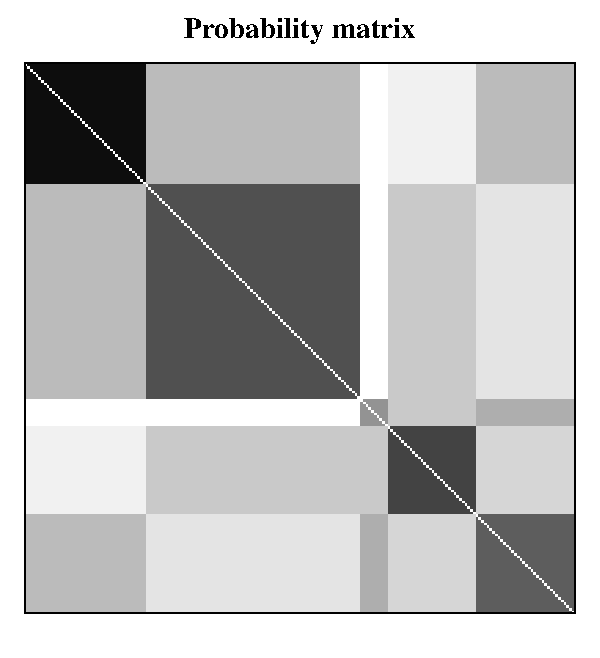
\includegraphics[height=\linewidth]{./Figures/SBM_P.pdf}
\end{subfigure}%
\begin{subfigure}{.45\textwidth}
  \centering
  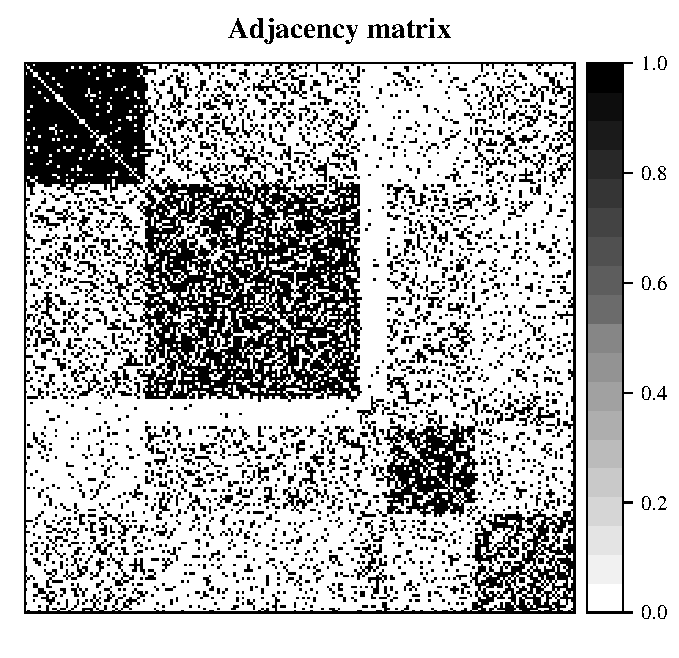
\includegraphics[height=\linewidth]{./Figures/SBM_A.pdf}
\end{subfigure}
\caption[Example illustrating the stochastic blockmodel]{Example illustrating the stochastic blockmodel. The parameters are given in Example~\ref{example:SBM}.
The left figure shows the probability matrix $P$ with $K = 5$ blocks and $n=200$ vertices and the right figure shows an adjacency matrix $A$ sampled under $\mathrm{SBM}(P)$.
While $A$ is a noisy version of $P$, much of the structure of $P$ is preserved in $A$, a property we will exploit in our estimation procedure.}
\label{fig:SBM_example}
\end{figure}

As discussed in Section~\ref{sec:RDPG}, the probability matrix $P$ in an RDPG is positive semidefinite. And now we argue that an SBM with a positive semidefinite $B$ can always be parameterized as an RDPG.
Firstly due to the positive semidefiniteness of $B$, we can decompose $B = \nu \nu^{\top}$ where $\nu \in \mathbb{R}^{K \times d}$. Define $\nu_1, \dots, \nu_K$ such that the rows of $\nu$ are given by $\nu_1^{\top}, \dots, \nu_K^{\top}$. Then $\nu_k$ can be regarded as the shared latent position for all vertices assigned to block $k$. Define $X = [X_1, \dots, X_n]^{\top} = [\nu_{\tau_1}, \dots, \nu_{\tau_n}]^{\top} \in \mathbb{R}^{n \times d}$. Then the SBM now can be parameterized as an RDPG since
\[
	\mathbb{P}(A_{ij} = 1) = B_{\tau_i, \tau_j} = \nu_{\tau_i}^{\top} \nu_{\tau_j}^{\phantom{\top}} = X_i^{\top} X_j \in [0, 1].
\]


\begin{definition} [SBM as RDPG]
\label{def:SBM_RDPG}
Consider an $\mathrm{RDPG}(\mathcal{X}, F)$ where $F$ is a distribution on $K$ point masses $\nu_1, \dots, \nu_K \in \mathcal{X}$ such that $\mathbb{P}(X_i = \nu_k) = \rho_k$ for $i \in [n]$ and $k \in [K]$, where the block proportion vector $\rho \in (0,1)^K$ with $\sum_{k=1}^K \rho_k = 1$. Then we denote this model by $\mathrm{SBM}(\rho, B)$ where $B = \nu^{\top} \nu$ with $\nu = [\nu_1, \dots, \nu_K]^{\top}$. Similarly, we can define $\tau \in [K]^n$ such that $X_i = \nu_{\tau_i}$. 
\end{definition}

For notational convenience we will refer to the sub-model of SBM with positive semidefinite $B$ as {\em{SBM}}.
As shown above, the SBM can be regard as an RDPG where all vertices in the same block have identical latent positions. In this work, we will always analyze SBM in an RDPG setting.


\begin{remark}
\label{remark:other_models}
As we mentioned, under the SBM, all vertices in the same block have identical latent positions. Rather than allowing vertices differ from each other as RDPG, SBM presumes all nodes within the same block have the same expected degree. To better describe complex networks in some situations, a bunch of generalizations of the SBM have been explored in order to incorporate the local variation of vertices to the block structure. \citet{airoldi2008mixed} proposed mixed membership stochastic blockmodels, which associates each vertex with multiple blocks with a probability vector rather than a single block as SBM requires. Also, in order to model variation of the expected degrees of different vertices within the same block, \citet{karrer2011stochastic} proposed degree-corrected SBM, which assigns additional parameters to each vertex to adjust the expected degree relatively. All these generalizations are trying to drag SBM towards RDPG a little bit so that the model can capture variations among vertices while keeping the community structure.
\end{remark}




\section{Weighted Random Graph Models}
\label{sec:weighted_graphs}

In this section, we shift our focus to the case where graphs are weighted and generalize the three models introduced in Section~\ref{sec:unweighted_graphs} respectively, i.e. the weighted independent edge model (WIEM) in Section~\ref{sec:WIEM}, the weighted random dot product graph model (WRDPG) in Section~\ref{sec:WRDPG}, and the weighted stochastic blockmodel (WSBM) as a WRDPG in Section~\ref{sec:WSBM}.

As a reminder, for weighted graphs, each edge is assigned with a positive real-valued weight, i.e. $\mathcal{A} = \mathbb{R}^{n \times n}_{\ge 0}$. So the adjacency matrices are not binary any more.


\subsection{Weighted Independent Edge Model}
\label{sec:WIEM}

As introduced in Section~\ref{sec:IEM}, under $\mathrm{IEM}(P)$, for $i, j \in [n]$ and $i < j$, the edge weight $A_{ij}$ is distributed from a Bernoulli distribution with parameter $P_{ij}$ independent of other edges.
We first extend IEM to weighted independent edge model (WIEM).

\begin{definition} [Weighted Independent Edge Model]
\label{def:WIEM}
Consider a one-parameter family of distributions $\mathcal{F} = \{ f_{\theta} : \theta \in \Theta \subset \mathbb{R} \}$. Let the graph parameters be a matrix $P \in \Theta^{n \times n} \subset \mathbb{R}^{n \times n}$.
Then under a {\em{weighted independent edge model} (WIEM)} with respect to $\mathcal{F}$, for $i, j \in [n]$ and $i < j$, the edge weight between vertex $i$ and vertex $j$ is distributed according to $f_{P_{ij}}$ independently.
\end{definition}

To see that an IEM is a special case of WIEM, let $\mathcal{F}$ be the collection of Bernoulli distributions and let the graph parameters be a symmetric and hollow matrix $P \in [0, 1]^{n \times n}$.
Note that the graphs considered in this paper are undirected without self-loops, thus the parameter matrix $P$ needs to be symmetric and hollow. However, for convenience, we still define the parameters to be an $n$-by-$n$ matrix while only $n \choose 2$ of them are effective.



\subsection{Weighted Random Dot Product Graph}
\label{sec:WRDPG}

As discussed in Section~\ref{sec:RDPG}, the connectivity between two vertices in a graph generally depends on some hidden properties of the corresponding vertices. Such property is well captured by LPM as well as RDPG, which is a special case of LPM. In this section, we generalize RDPG to a weighted version so that it can model weighted graphs. 

\begin{definition}[Weighted Random Dot Product Graph]
Consider a collection of one-parameter distributions $\mathcal{F} = \{ f_{\theta}, \theta \in \Theta \subset \mathbb{R} \}$. The {\em{weighted random dot product graph (WRDPG)}} with respect to $\mathcal{F}$ is defined as following: Let $X \in \mathbb{R}^{n \times d}$ be such that $X = [X_1, X_2, \dotsc, X_n]^{\top}$, where $X_i \in \mathbb{R}^d$ for all $i \in [n]$. The matrix $X$ is random and satisfies $\mathbb{P}( X_i^{\top} X_j \in \Theta ) = 1$ for all $i, j \in [n]$. Conditioned on $X$, $A_{ij}$ follows distribution $f_{\theta} \in \mathcal{F}$ with parameter $\theta = X_i^{\top} X_j$ independent of others for $i, j \in [n]$ and $i < j$.
\end{definition}

Under the WRDPG defined above, the parameter matrix $P = X X^T \in \mathbb{R}^{n \times n}$ is automatically symmetric because the link function is inner product. Moreover, to have symmetric graphs without self-loops, only $A_{ij}$ ($i < j$) are sampled while leaving the diagonals of $A$ to be all zeros.

After such extension, WRDPG inherits some properties from RDPG naturally, for example the positive defininteness of $P$, non-identifiability, etc. And similarly, since $P$ is still the outer product of the latent positions $X$ in WRDPG, it also motivates the low-rank estimator based on spectral decomposition for weighted graphs which will be discussed in later sections.




\subsection{Weighted Stochastic Blockmodel}
\label{sec:WSBM}

\begin{definition} [Weighted Stochastic Blockmodel]
\label{def:SBM}
Consider a collection of one-parameter distributions $\mathcal{F} = \{ f_{\theta}, \theta \in \Theta \subset \mathbb{R} \}$. A $K$-block {\em{weighted stochastic blockmodel (WSBM)}} with respect to $\mathcal{F}$ is defined as following: Let block probability matrix be $B \in \Theta^{K \times K}$, and let the vector of block memberships be $\tau \in [K]^n$, where for each $i \in [n]$, $\tau_i = k$ means vertex $i$ is a member of block $k$. Then $A_{ij}$ follows distribution $f_{\theta} \in \mathcal{F}$ with parameter $\theta = B_{ij}$ independent of others for $i, j \in [n]$ and $i < j$.
\end{definition}

WSBM can be defined in a similar way in the scenario when the block probability matrix $B$ and block membership vector $\tau$ are random. As mentioned in Section~\ref{sec:SBM}, all analysis for unweighted graphs is based on RDPG setting. Likewise, in this section we will represent WSBM as WRDPG. Because of the structure of WRDPG, in order to consider WSBM as a WRDPG, the block probability matrix $B$ needs to be positive semidefinite. From now on, we will denote the sub-model of WSBM with positive semi-definite $B$ as the WSBM.

\begin{definition} [WSBM as WRDPG]
\label{def:SBM_RDPG}
Consider a WRDPG with respect to $\mathcal{F}$ where each latent position $X_i$ can take one of the $K$ possible values $\nu_1, \dots, \nu_K$ such that $\mathbb{P}(X_i = \nu_k) = \rho_k$ for $i \in [n]$ and $k \in [K]$, where the block proportion vector $\rho \in (0,1)^K$ with $\sum_{k=1}^K \rho_k = 1$. Then this is a WSBM with respect to $\mathcal{F}$ where $B = \nu^{\top} \nu$ with $\nu = [\nu_1, \dots, \nu_K]^{\top}$. Similarly, we can define $\tau \in [K]^n$ such that $X_i = \nu_{\tau_i}$. 
\end{definition}

As shown above, the WSBM can be regard as a WRDPG where all vertices in the same block have identical latent positions. In later sections when considering weighted graphs, we will always analyze WSBM in a WRDPG setting.


















%!TEX root = root.tex

\chapter{A Law of Large Graphs}
\label{chap:llg}

Estimation of the mean of a population based on samples is at the core of statistics.
The sample mean, motivated by the law of large numbers and the central limit theorem, has its place as one of the most important statistics for this task.
In modern settings, we take averages almost everywhere, from data in Euclidean space to more complex objects like images, shapes, and documents.
In this chapter we consider the challenges of estimating a population mean based on a sample of graphs, for example the human brains as represented by their structural connectomes. 

The mean of a population of graphs is a high dimensional object, consisting of $O(n^2)$ parameters for graphs with $n$ vertices.
When the number of samples $m$ is much smaller than $n^2$, or even $n$, estimating such high dimensional estimands using naive unbiased methods often leads to inaccurate estimates with very high variance.
Furthermore, using these estimates for subsequent inference tasks such as testing can lead to low power and accuracy.
By exploiting a bias-variance trade-off, it is often fruitful to develop estimators which have some bias but greatly reduced variance.
When these estimators are biased towards low-dimensional structures which well approximate the full dimensional population mean, major improvements can be realized \citep{trunk1979problem}.

In a striking result, \citet{stein1956inadmissibility} and \citet{james1961estimation} showed that even the arithmetic mean can be dominated by another procedure.
In particular, James and Stein showed that the sample mean for a multivariate normal distribution with at least three dimensions has strictly higher risk than a procedure that introduces shrinkage, and can be strictly improved by carefully biasing the  estimate towards any given fixed point. 
Twenty-seven years later, \citet{gutmann1982stein} proved that this phenomenon cannot occur when the sample spaces are finite, as is the case for graphs.
However, while there must be some cases where the sample mean is preferred, this does not mean that other estimators should not be considered.
In many situations where other structural information is hypothesized, other estimators may be preferable.

In complex data settings such as shape data, language data, or graph data, we also must take care in how we define the mean.
For a population, we define the mean graph as the weighted adjacency matrix with weights given by the proportion of times the corresponding edge appears in the population. 
This definition naturally extends the definition of the mean for standard Euclidean data.
As with real valued data, one may want to define the mean of a population of graphs to be a graph.
This is captured in the notion of the median graph \citep{jiang2001median}, however, this may be too restrictive for populations of graphs where there is high variation in which edges appear. 
As we will describe below, our definition of the mean graph is the expectation of the adjacency matrix.

This population mean is becoming an important object for statistical inference.
For example, \citet{ginestet2014hypothesis} proposed a way to test if there is a difference between the distributions for two groups of networks.  
While hypothesis testing is the end goal of their work, estimation is a key intermediate step which may be improved by accounting for underlying structure in the mean matrix. 
Thus, improving the estimation procedures for the mean graph is not only important by itself, but also can be applied to help improve other statistical inference procedures.

To better illustrate the idea, we take the CoRR brain graphs with Desikan atlases as an example. The dataset contains 454 brain scans with 70 vertices. Each vertex represents a region defined by the Desikan atlases, while an edge exists between two vertices if there is at least one white-matter tract connecting the corresponding regions of the brain. More details about this dataset are given in Section~\ref{section:data}. By observing $m$ graphs sampled from the 454 graphs, our goal is to estimate the mean graph of the population $P$, defined as the entry-wise mean of all the 454 graphs. We plot the population mean graph $P$ on the left panel in Figure~\ref{fig:Matrix_desikan_m5}.


\begin{figure}[!tbp]
\centering
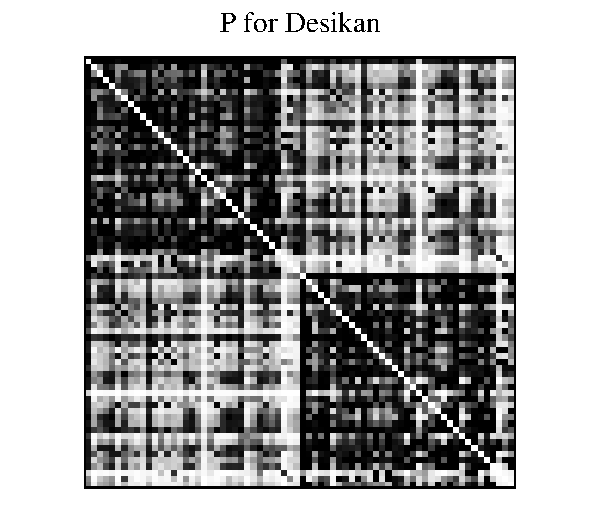
\includegraphics[height=.2\textheight]{./Figures/P_desikan.pdf} \hspace{-35pt}
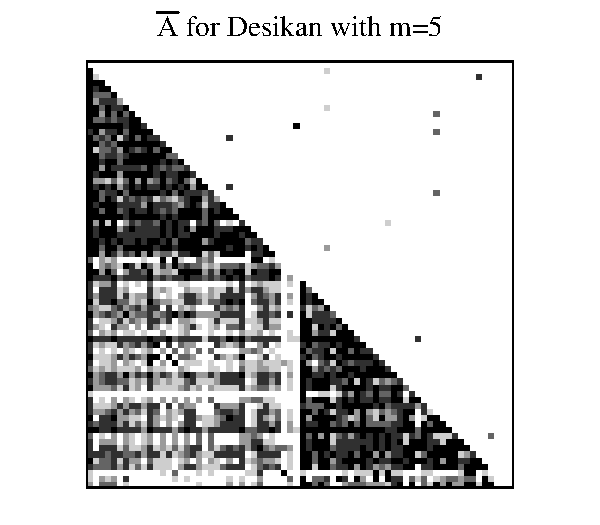
\includegraphics[height=.201\textheight]{./Figures/Abar_desikan_m5.pdf} \hspace{-35pt}
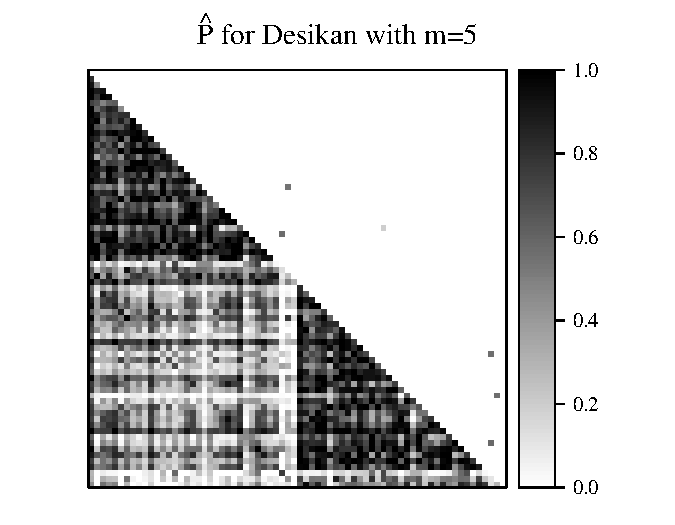
\includegraphics[height=.205\textheight]{./Figures/Phat_desikan_m5.pdf}
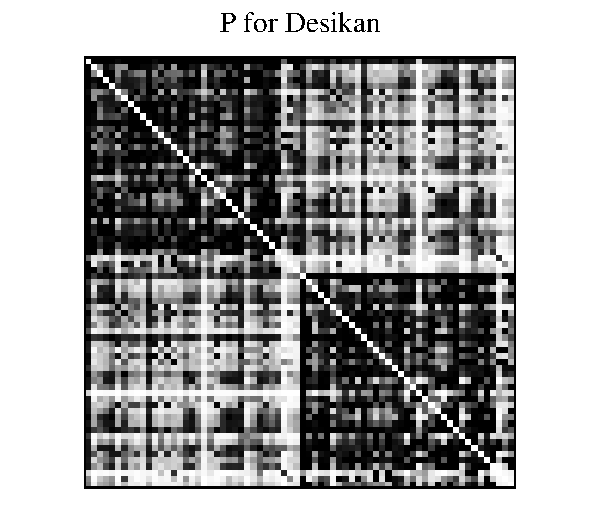
\includegraphics[height=.2\textheight]{./Figures/P_desikan.pdf} \hspace{-35pt}
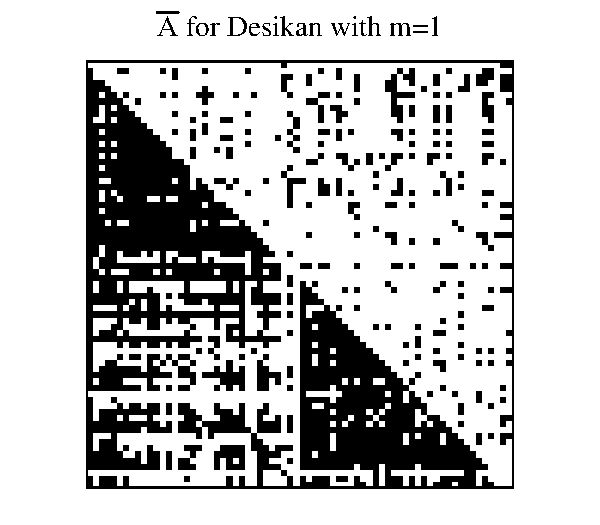
\includegraphics[height=.201\textheight]{./Figures/Abar_desikan_m1.pdf} \hspace{-35pt}
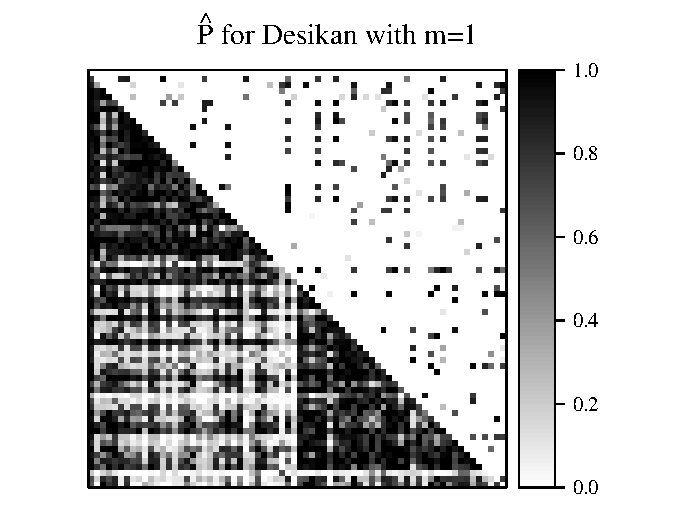
\includegraphics[height=.205\textheight]{./Figures/Phat_desikan_m1.pdf}
\caption[Heat maps of the population mean, the sample mean, and the low-rank estimator]{Heat maps of the population mean $P$, the sample mean $\bar{A}$, and the estimator $\hat{P}$ based on sample sizes $m = 1$ and $m = 5$.
The three heat maps in the upper level indicate the population mean for the $454$ graphs (left), sample mean for the 5 sampled graphs (center), and $\hat{P}$ for the same 5 sampled graphs with dimension $d=11$ selected using the Zhu and Ghodsi method (right). Details about how to construct $\hat{P}$ are discussed in Section~\ref{sec:LLG_phat}.
Darker pixels indicate a higher probability of an edge between the given vertices.
By calculating the mean squared error based on this sample, we can see that $\hat{P}$ (with mean squared error equals $0.015$) outperforms $\bar{A}$ (with mean squared error equals $0.016$), with a 3\% relative improvement.
In order to see where the improvements are clearly, in the upper triangular of the heat maps for $\bar{A}$ and $\hat{P}$, we highlight the edges (18 edges highlighted for $\bar{A}$ and 6 for $\hat{P}$) which have absolute estimation error larger than $0.4$.
In the lower level, we plot three heat maps in the similar way based on sample size $m = 1$. For this specific sampled graph, $\hat{P}$ is calculated with dimension $d = 12$. A clearly smoothing effect can be seen in the heat map of $\hat{P}$ (with mean squared error equals $0.049$), which leads to a 53\% relative improvement compared to $\bar{A}$ (with mean squared error equals $0.104$). Similarly, we use the same absolute estimation error threshold $0.4$ and highlight 504 edges for $\bar{A}$ and 234 edges for $\hat{P}$.}
\label{fig:Matrix_desikan_m5}
\end{figure}



The element-wise sample mean is a reasonable estimator if we consider the general independent edge model (IEM) \citep{bollobas2007phase} introduced in Section~\ref{sec:IEM} without taking any additional structure into account. 
However, with only a small sample size, such as when the sample size is much less than the number of vertices, it does not perform very well.
Now take a sample of size $m=5$ in the CoRR dataset example with Desikan atlases mentioned above, then we calculate the entry-wise sample mean $\bar{A}$ and plot it in the top middle panel of Figure~\ref{fig:Matrix_desikan_m5}. Darker pixels indicate a higher probability of an edge between the given vertices.
We can see $\bar{A}$ gives a fair estimate of $P$. However, there are still an amount of edges being estimated very inaccurately. In order to see these inaccurate estimates clearly, in the upper triangular of the heat maps for $\bar{A}$, we highlight the 18 edges which have absolute estimation error larger than $0.4$ based on the same color scale.
When the sample size is small, the performance of $\bar{A}$ degrades due to its high variances. Such phenomenon is most obvious when we decrease the sample size from $m = 5$ to $m = 1$.
In the bottome middle panel of Figure~\ref{fig:Matrix_desikan_m5}, we plot the heat map of $\bar{A}$ based on sample size $m = 1$. Since there is only one observed graph, $\bar{A}$ is binary and thus very bumpy. Similarly, we use the same absolute estimation error threshold $0.4$ and highlight 504 edges in the upper triangular.
Intuitively, an estimator incorporating structure in the distribution of graphs, assuming the estimator is computationally tractable, is preferable to the entry-wise sample mean. 
In general, we do not have any knowledge about this structure so it can be hard to take advantage of in practice.



One of the most important structures in graphs is the community structure in which vertices are clustered into groups that share similar connectivity structure. The stochastic blockmodel (SBM) \citep{holland1983stochastic} introduced in Section~\ref{sec:SBM} is one model that captures this structural property and is widely used in modeling networks. From population mean $P$ plotted in Figure~\ref{fig:Matrix_desikan_m5}, we can see the brain is a 2-block model at the highest level, representing the two hemispheres.
More generally, the latent positions model (LPM) \citep{hoff2002latent} introduced in Section~\ref{sec:RDPG}, provides a way to parameterize the graph structure by latent positions associated with each vertex. 
Latent position models can capture strong community structure like the stochastic blockmodel, but may also allow for more variance within communities and other structures.
One example of an LPM which captures this middle ground is the random dot product graph (RDPG) \citep{young2007random, nickel2008random} introduced in Section~\ref{sec:RDPG} which motivates our estimator. It generalizes the positive semidefinite SBM by allowing for mixed membership and degree corrections.
% In this paper, we analyze our estimator in terms of RDPG specifically.

Using estimates of the latent positions based on a truncated eigen-decomposition of the adjacency matrix, we propose an estimator which captures the low-rank structure of the mean graph for the RDPG model. Details about this estimator are discussed in Section~\ref{sec:LLG_phat}.
These estimates will improve performance since they will be biased towards the low-rank structure of the RDPG model and will have much lower overall variance than naive element-wise sample means. Here we consider the same random sample of size $m=5$ based on the Desikan atlas in Figure~\ref{fig:Matrix_desikan_m5} and plot the estimate $\hat{P}$ in the top right panel. Note that compared to the sample mean $\bar{A}$ (with mean squared error equals $0.016$), $\hat{P}$ (with mean squared error equals $0.015$) has a finer gradient of values which in this case leads to a 3\% relative improvement in estimation of the true probability matrix $P$. In order to see where the improvements are clearly, in the upper triangular of the heat map for $\hat{P}$, we also highlight the 6 edges which have absolute estimation error larger than $0.4$, where 18 edges are highlighted for $\bar{A}$ based on the same threshold. 
The smoothing effect is much more obvious when we decrease the sample size from $m = 5$ to $m = 1$. In the lower level of Figure\ref{fig:Matrix_desikan_m5}, we plot the heat map of $\hat{P}$ based on sample size $m = 1$. From the figure, we can see that $\hat{P}$ smooths the estimate, especially for edges across the two hemispheres, in the lower left and corresponding upper right block (which is not shown in the heat map). Based on the calculations, $\hat{P}$ (with mean squared error equals $0.049$) outperforms $\bar{A}$ (with mean squared error equals $0.104$), with a 53\% relative improvement. Similarly, we use the same absolute estimation error threshold $0.4$ and highlight the 234 edges for $\hat{P}$.


In this chapter, we show via theory, simulations, and real data analysis that the low-rank estimator frequently outperforms the element-wise sample mean, especially in small sample sizes.


In Section~\ref{sec:LLG_model}, we outline the model which we consider for our theorems and simulations, and in Section~\ref{sec:LLG_estimator} we describe the entry-wise sample mean and introduce our specific low-rank estimator, which accounts for the unknown dimension and attempts to correct for other issues found in real world problems.
Our main theoretical results are presented in Section~\ref{sec:LLG_theoretical_result}. And then we present simulations results for the stochastic blockmodel in Section~\ref{sec:sbm_sim}, an investigation of a connectome dataset in Section~\ref{sec:LLG_corr_data}, and a synthetic data analysis in Section~\ref{sec:sim_iem}.

%We conclude with a discussion of these results in Section~\ref{sec:LLG_discussion}  and with details on our proposed method and the data which is analyzed in Section~\ref{sec:LLG_method}.





\section{Model}
\label{sec:LLG_model}

This chapter considers the scenario of having $m$ unweighted graphs, represented as adjacency matrices, $A^{(1)},A^{(2)},\dotsc,A^{(m)}$, each having $n$ vertices with $A^{(t)}\in\{0,1\}^{n \times n}$ for $t \in [m]$.
We assume there is a known correspondence for vertices across different graphs, so that vertex $i$ in graph $t$ corresponds to vertex $i$ in graph $t'$ for any $i \in [n]$, $t, t' \in [m]$.
The graphs we consider are undirected and unweighted with no self-loops, so each $A^{(t)}$ is a binary symmetric matrix with zeros along the diagonal. 

For the purpose of this paper, we also assume that the graphs are sampled independently and identically from some distribution.
To this end, the mean graph we are trying to estimate is the expectation of each adjacency matrix.
\begin{definition}[Mean Graph]
\label{def:mean_graph}
Suppose that $A^{(1)},\dotsc,A^{(m)}\stackrel{iid}{\sim} \mathcal{G}$ for some random graph distribution $\mathcal{G}$, with $A^{(t)}\in\{0,1\}^{n \times n}$ for $t \in [m]$.
The {\em mean graph} is defined as $\Ex[A^{(1)}]$, where since the graphs are identically distributed $\Ex[A^{(t)}]=\Ex[A^{(t')}]$ for $t, t' \in [m]$.
\end{definition}

In this chapter, we consider the scenario that all $m$ graphs follow the same SBM. Since the vertex correspondence is assumed across graphs, the block memberships $\tau_i$ are firstly drawn iid from a categorical distribution with block membership probabilities given by $\rho\in[0,1]^K$ and this will keep the same for all $m$ graphs to be sampled.
Denote block probability matrix $B = \nu \nu^{\top} \in [0, 1]^{K \times K}$. 
By Definition~\ref{def:mean_graph}, the mean of the collection of graphs generated from this SBM is $P \in [0, 1]^{n \times n}$, where $P_{ij} = B_{\tau_i, \tau_j}$.
Then $m$ graphs on $n$ vertices $A^{(1)}, \cdots, A^{(m)}$ are sampled independently from the SBM conditioned on $\tau$.





\section{Methods}
\label{sec:LLG_method}

Before we start introducing our estimators for $P$, in this section we focus on several methods which are key components for constructing the estimators later.

\subsection{Adjacency Spectral Embedding}
\label{sec:ASE}

We first introduce the adjacency spectral embedding (ASE), which is our most important tool for exploiting the low-rank property.

\begin{definition} [Adjacency Spectral Embedding]
\label{def:ASE}
For a symmetric $n$-by-$n$ matrix $A$, let its eigen-decomposition be $\hat{U} \hat{S} \hat{U}^{\top} + \tilde{U}\tilde{S}\tilde{U}^{\top}$, where $\hat{S}$ is a diagonal matrix with non-increasing entries along the diagonal corresponding to the largest $d$ eigenvalues of $A$, and $\hat{U}$ has columns given by the corresponding eigenvectors. Similarly, $\tilde{S}$ is the diagonal matrix with non-increasing entries along the diagonal corresponding to the rest $n - d$ eigenvalues of $A$, and $\tilde{U}$ has the columns given by the corresponding eigenvectors.
Then the $d$-dimensional {\em{adjacency spectral embedding (ASE)}} of $A$ is defined as $\hat{X}=\hat{U} \hat{S}^{1/2}\in \mathbb{R}^{n \times d}$.
\end{definition}

Consider the probability matrix $P$ in an RDPG setting with latent positions $X \in \mathbb{R}^{n \times d}$, i.e. $P = X X^{\top}$. Then the $d$-dimensional ASE of $P$ exactly recovers its latent positions $X$.
Moreover, \citet{sussman2014consistent} showed that the ASE of the adjacency matrix $A$ under RDPG gives good estimates of the latent vectors for each vertex under appropriate conditions.




\subsection{Choosing Dimension}
\label{sec:dim_select}
Often in dimensionality reduction techniques, the choice for dimension $d$, relies on analyzing the set of the ordered eigenvalues, looking for a ``gap'' or ``elbow'' in the scree-plot. \citet{zhu2006automatic} present an automated method for finding this gap in the scree-plot that takes only the ordered eigenvalues as an input and uses Gaussian mixture modeling to find these gaps.
The mixture modeling results in multiple candidate dimensions or elbows, and our analysis indicated that underestimating the dimension is much more harmful than overestimating the dimension.
For this reason, we used the 3rd elbow in the experiments performed for this work.

Universal Singular Value Thresholding (USVT) is a simple estimation procedure proposed in \citet{chatterjee2015matrix} that can work for any matrix that has ``a little bit of structure''. 
In our setting, it selects the dimension $d$ as the number of singular values that are greater than a constant $c$ times $\sqrt{n/m}$.
The specific constant $c$ must be selected carefully based on the mean and variance of the entries, and since again we found that overestimating the dimension was not overly harmful, we chose a relatively small value of $c=0.7$.

Overall, selecting the appropriate dimension is a challenging task and numerous methods could be applied successfully depending on the setting.
On the other hand, we have observed that in our setting, many dimensions will yield nearly optimal mean squared errors. 
Thus efforts to ensure the selected dimension is in the appropriate range are more important than finding the best dimension.





\subsection{Graph Diagonal Augmentation}
\label{sec:diag_aug}
The graphs examined in this work have no self-loops and thus the diagonal entries of the adjacency matrix and the mean graph are all zero.
However, when computing the low-rank approximation, these structural zeros lead to increased errors in the estimation of the mean graph. 
While this problem has been investigated in the single graph setting, with multiple graphs, the problem is exacerbated since the variance of the other entries is lower, so the relative impact of the bias in the diagonal entries is higher.
Moreover, the sum of eigenvalues of the hollow matrix will be zero, leading to an indefinite matrix, which violates the positive semi-definite assumption. So it is important to remedy the situation that we don't observe the diagonal entries.

\citet{marchette2011vertex}  proposed the simple method of imputing the diagonals to be equal to the average of the non-diagonal entries for the corresponding row.
Earlier, \citet{scheinerman2010modeling} proposed using an iterative method to impute the diagonal entries.
In this work, we combine these two ideas by first using the row-average method  (see Step 3 of Algorithm~\ref{algo:LLG_basic}) and then using one step of the iterative method (see Step 6 of Algorithm~\ref{algo:LLG_basic}), which will be discussed in Section~\ref{sec:LLG_estimator}.
Note that when computing errors, we omit the diagonal entries since these are known to be zero.








\section{Estimators}
\label{sec:LLG_estimator}

In this section, we present two estimators, the standard element-wise sample mean $\bar{A}$, and a low-rank estimator $\hat{P}$. We describe the low-rank aspects of this estimator as well as further important details regarding diagonal augmentation and dimension estimation in this section.


\subsection[Element-wise sample mean]{Element-wise sample mean $\bar{A}$}
\label{sec:LLG_abar}

The most natural estimator to consider is to take the average of the observed adjacency matrices which yields the element-wise sample mean.
This estimator, defined as $\bar{A}=\frac{1}{m}\sum_{t=1}^m A^{(t)}$, is the  maximum likelihood estimator (MLE) for the mean graph $P$ if the graphs are sampled from an IEM distribution.
It is unbiased so $\Ex[\bar{A}]=P$ with entry-wise variance $\mathrm{Var}(\bar{A}_{ij}) = P_{ij} (1-P_{ij})/m$. Moreover, $\bar{A}$ is the uniformly minimum-variance unbiased estimator, so it has the smallest variance among all unbiased estimators and enjoys the many asymptotic properties of the MLE as $m\to \infty$ for fixed $n$.
However, if graphs with a large number of vertices are of interest, there are no useful asymptotic properties for $\bar{A}$ as the number of vertices $n$ becomes large for fixed $m$.

Additionally, $\bar{A}$ doesn't exploit any graph structure.
If the graphs are distributed according to an RDPG or SBM, then $\bar{A}$ is no longer the maximum likelihood estimator since it is not guaranteed to satisfy the properties of the mean graph for that model.
The performance can be especially poor when the sample size $m$ is small, such as when $m \ll n$.
For example, when $m = 1$, $\bar{A}$ is simply the binary adjacency matrix $A^{(1)}$, which is an inaccurate estimate for an arbitrary $P$ compared to estimates which exploit underlying structure, such as occurs for the RDPG.



\subsection[Low-Rank Estimator]{Low-Rank Estimator $\hat{P}$}
\label{sec:LLG_phat}

Motivated by the low-rank structure of the RDPG mean matrix, we propose the estimator $\hat{P}$ based on the spectral decomposition of $\bar{A}$ which yields a low rank approximation of $\bar{A}$.
This estimator is similar to the estimator proposed by \citet{chatterjee2015matrix} but additionally
we propose adjustments to canonical low-rank methods which serve to improve the performance for the specific task of estimating the mean graph. 
Additionally, we consider an alternative dimension selection technique as discussed in Section~\ref{sec:dim_select}.
To summarize, our overall strategy to computer $\hat{P}$ is described in Algorithm \ref{algo:LLG_basic}. The key component of this algorithm is the low-rank estimator. Details of this vital step to compute the actual low-rank approximation is in Algorithm \ref{algo:LLG_lowrank}.

\begin{algorithm}[H]
\caption{Algorithm to compute $\hat{P}$}
\label{algo:LLG_basic}
\begin{algorithmic}[1]
\REQUIRE Adjacency matrices $A^{(1)}, A^{(2)}, \dots, A^{(m)}$, with each $A^{(t)} \in \{0,1\}^{n \times n}$
\ENSURE Estimate $\hat{P}\in[0,1]^{n \times n}$
\STATE Calculate the sample mean $\bar{A} = \frac{1}{m}\sum\limits_{t = 1}^m A^{(t)}$;
\STATE Calculate the scaled degree matrix $D^{(0)} = \mathrm{diag}(\bar{A} \bm{1})/(n-1)$;
\STATE Select the dimension $d$ based on the eigenvalues of $\bar{A} + D^{(0)}$; (see Section~\ref{sec:dim_select})
\STATE Set $\tilde{P}^{(0)}$ to $\mathrm{lowrank}_d(\bar{A} + D^{(0)})$; (see Algorithm~\ref{algo:LLG_lowrank})
\STATE Set $D^{(1)}$ to $ \mathrm{diag}(\tilde{P}^{(0)})$, the diagonal matrix with diagonal matching $\tilde{P}^{(0)}$; 
\STATE Set $\tilde{P}^{(1)}$ to $\mathrm{lowrank}_d(\bar{A} + D^{(1)})$; (see Algorithm~\ref{algo:LLG_lowrank})
\STATE Set $\hat{P}$ to $\tilde{P}^{(1)}$ with values $<0$ set to $0$ and values $>1$ set to $1$.
\end{algorithmic}
\end{algorithm}


For a given dimension $d$ we consider the estimator $\mathrm{lowrank}_d(\bar{A})$ defined as the best rank-$d$ positive semidefinite approximation of $\bar{A}$.
Since the graphs are symmetric, we can compute the eigen-decomposition of $\bar{A}$ as $\hat{U} \hat{S} \hat{U}^{\top} + \tilde{U}\tilde{S}\tilde{U}^{\top}$, where $\hat{S}$ is a diagonal matrix with non-increasing entries along the diagonal corresponding to the largest $d$ eigenvalues of $\bar{A}$, and $\hat{U}$ has columns given by the corresponding eigenvectors. Similarly, $\tilde{S}$ is the diagonal matrix with non-increasing entries along the diagonal corresponding to the rest $n - d$ eigenvalues of $\bar{A}$, and $\tilde{U}$ has the columns given by the corresponding eigenvectors.
The $d$-dimensional adjacency spectral embedding (ASE) of $\bar{A}$ is given by $\hat{X}=\hat{U} \hat{S}^{1/2}\in \mathbb{R}^{n \times d}$.
For an RDPG, the rows of $\hat{X}$ are estimates of the latent vectors for each vertex \citep{sussman2014consistent}.
Using the adjacency spectral embedding, we have the low-rank approximation of $\bar{A}$ to be $\hat{X} \hat{X}^{\top}=\hat{U}\hat{S}\hat{U}^{\top}$.
Algorithm~\ref{algo:LLG_lowrank} gives the steps to compute this low-rank approximation for a general symmetric matrix $A$.

\begin{algorithm}[H]
\caption{Algorithm to compute the rank-$d$ approximation of a matrix.}
\label{algo:LLG_lowrank}
\begin{algorithmic}[1]
\REQUIRE Symmetric matrix $A\in \mathbb{R}^{n \times n}$ and dimension $d \leq n$.
\ENSURE $\mathrm{lowrank}_d(A)\in \mathbb{R}^{n \times n}$
\STATE Compute the algebraically largest $d$ eigenvalues of $A$, $s_1\geq s_2\geq \dotsc\geq s_d$ and corresponding unit-norm eigenvectors $u_1,u_2,\dotsc,u_d\in \mathbb{R}^n$;
\STATE Set $\hat{S}$ to the $d\times d$ diagonal matrix $\mathrm{diag}(s_1,\dotsc,s_d)$;
\STATE Set $\hat{U} = [u_1,\dotsc,u_d]\in \mathbb{R}^{n \times d}$;
\STATE Set $\mathrm{lowrank}_d(A)$ to $\hat{U}\hat{S}\hat{U}^{\top}$;
\end{algorithmic}
\end{algorithm}

To compute our estimator $\hat{P}$, we also need to specify what rank $d$ to use and there are various ways of dealing with dimension selection. 
In this work, we use an elbow selection method proposed in \citet{zhu2006automatic} and the universal singular value thresholding (USVT) method \citep{chatterjee2015matrix}. 
Details for these methods are discussed in Section~\ref{sec:dim_select}.

Moreover, since the adjacency matrices are hollow, with zeros along the diagonal, there is a missing data problem that leads to inaccuracies if we compute $\hat{P}$ based only on $\bar{A}$. 
To compensate for this issue, we use an iterative method developed in \citet{scheinerman2010modeling}. 
Details are discussed in Section~\ref{sec:diag_aug}.

Algorithm~\ref{algo:LLG_basic} gives the steps involved to compute the low-rank estimate $\hat{P}$. For convenience, here we consider Example~\ref{example:SBM} again.
In Figure~\ref{fig:SBM_example_full}, the upper left figure shows the probability matrix $P$ with $K = 5$ blocks and $n=200$ vertices and the upper right figure shows an adjacency matrix $A$ sampled under $\mathrm{SBM}(P)$, which repeats Figure~\ref{fig:SBM_example}.
The bottom panels of Figure~\ref{fig:SBM_example_full} demonstrate the two estimators $\hat{P}$ and $\bar{A}$ for the stochastic blockmodel given by the upper left panel. 
The estimates are based on a sample of size $m=3$ and in this instance visual inspection demonstrates that $\hat{P}$ performs much better than $\bar{A}$.
As we will see in the succeeding sections, this procedure will frequently yield improvements in estimation as compared to using the sample mean $\bar{A}$.
While this is unsurprising for random dot product graphs, where we are able to show theoretical results to this effect, we also see this effect for connectome data and more general independent edge graphs.
In the following sections, we explore this estimator in the context of the stochastic blockmodel discussed in Section~\ref{sec:LLG_model}.

\begin{figure}
\centering
\begin{subfigure}{.45\textwidth}
  \centering
  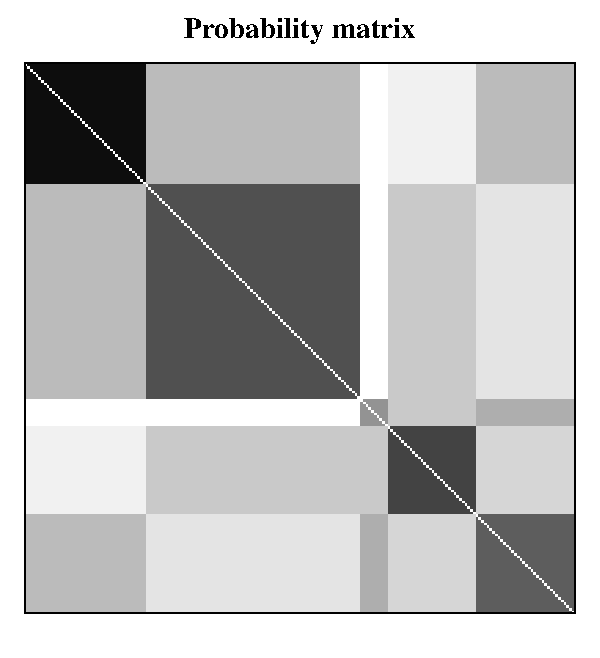
\includegraphics[height=\linewidth]{./Figures/SBM_P.pdf}
\end{subfigure}%
\begin{subfigure}{.45\textwidth}
  \centering
  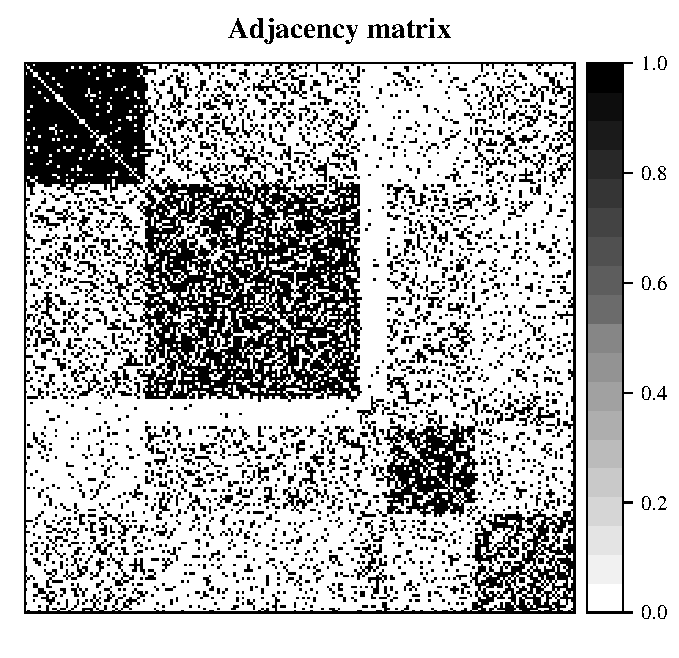
\includegraphics[height=\linewidth]{./Figures/SBM_A.pdf}
\end{subfigure}
\begin{subfigure}{.45\textwidth}
  \centering
  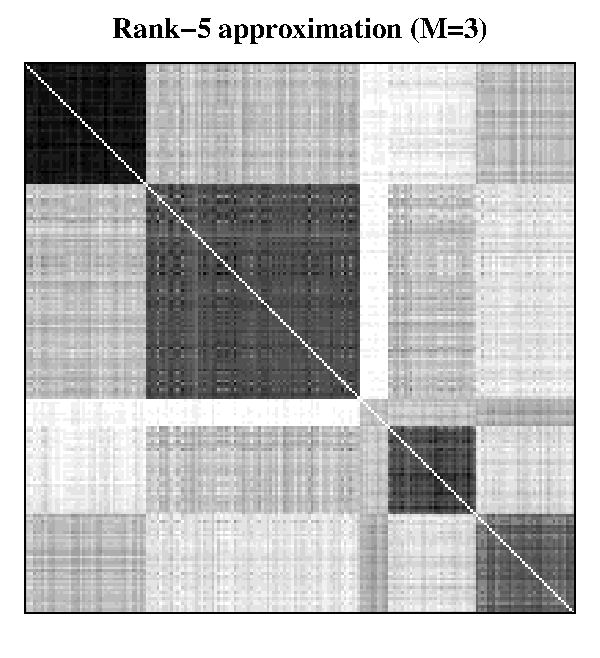
\includegraphics[height=\linewidth]{./Figures/SBM_Phat.pdf}
\end{subfigure}%
\begin{subfigure}{.45\textwidth}
  \centering
  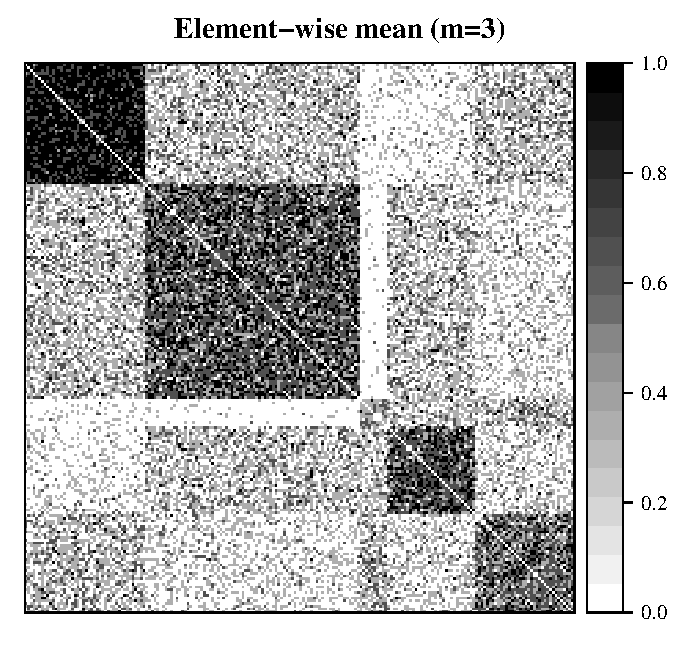
\includegraphics[height=\linewidth]{./Figures/SBM_Abar.pdf}
\end{subfigure}
\caption[Example illustrating different estimates under the stochastic blockmodel]{Example illustrating different estimates under the stochastic blockmodel.
The top left figure shows the mean graph $P$ with $K = 5$ blocks and $n=200$ vertices and the top right figure shows an adjacency matrix $A$ sampled according to the probabilities from $P$.
While $A$ is a noisy version of $P$, much of the structure of $P$ is preserved in $A$, a property we will exploit in our estimation procedure.
Based on three graphs sampled independently and identically according to the probability matrix $P$, we construct the element-wise mean $\bar{A}$, shown in the lower right panel (see Section~\ref{sec:LLG_abar}).  
Finally, by taking a rank-5 approximation of $\bar{A}$ and thresholding the values to be between $0$ and $1$, we construct our proposed estimate $\hat{P}$, shown in the lower left panel (see Section~\ref{sec:LLG_phat}).
By visual inspection, it is clear that the low-rank estimate $\hat{P}$ more closely approximates the probability matrix $P$ as compared to $\bar{A}$.
}
\label{fig:SBM_example_full}
\end{figure}








\section{Theoretical Results}
\label{sec:LLG_theoretical_result}

To estimate the mean of a collection of graphs, we consider the two estimators from Section~\ref{sec:LLG_estimator}: the entry-wise sample mean $\bar{A}$ and the low-rank $\hat{P}$ motivated by RDPG.
We evaluate our estimators in terms of mean squared error, either $\mathrm{MSE}(\hat{P}_{ij})=\Ex[\hat{P}_{ij}-P_{ij}]^2$ or $\mathrm{MSE}(\bar{A})=\Ex[\bar{A}_{ij}-P_{ij}]^2$.
While we can directly compare the difference in mean squared errors between the two estimators, it is frequently useful to consider the relative efficiency between two estimators.

\begin{definition} [Relative Efficiency]
\label{def:RE}
For two estimators $\hat{\theta}_1$ and $\hat{\theta}_2$, the {\em{relative efficiency (RE)}} between two estimators are defined as
\[
	\mathrm{RE}(\hat{\theta}_1, \hat{\theta}_2) = \frac{\mathrm{MSE}(\hat{\theta}_2)}{\mathrm{MSE}(\hat{\theta}_1)}.
\]
\end{definition}

In our case, this is $\mathrm{RE}(\bar{A}_{ij},\hat{P}_{ij}) = \frac{\mathrm{MSE}(\hat{P}_{ij})}{\mathrm{MSE}(\bar{A}_{ij})}$, with values above 1 indicating $\bar{A}$ should be preferred while values below 1 indicate $\hat{P}$ should be preferred.
Relative efficiency is a useful metric for comparing estimators because it will frequently be invariant to the scale of the noise in the problem and hence is more easily comparable across different settings.

In this section, we analyze the performance of these two estimators under the SBM by computing the entry-wise relative efficiency. 
We also consider the {\em{asymptotic relative efficiency (ARE)}}, which is the limit of the relative efficiency as the number of vertices $n \to\infty$ but with the number of graphs $m$ fixed, and the scaled relative efficiency, $n \cdot \mathrm{RE}(\bar{A}_{ij},\hat{P}_{ij}) $ which in our case normalizes the relative efficiency so that the asymptotic scaled relative efficiency is non-zero and finite. Somewhat surprisingly, we will see that the asymptotic relative efficiency will not depend on this fixed sample size $m$.

For this asymptotic framework, we assume the block memberships $\tau_i$ are drawn iid from a categorical distribution with block membership probabilities given by $\rho\in[0,1]^K$.
In particular, this implies that for each block $k$, the proportion $|\{i:\tau_i=k\}|/n$ of vertices in block $k$ will converge to $\rho_k$ as $n \to\infty$ by the law of large numbers.
We will also assume that for a given $n$, the block membership probabilities are fixed for all graphs.
Denote block probability matrix $B = \nu \nu^{\top} \in [0, 1]^{K \times K}$. 
By definition, the mean of the collection of graphs generated from this SBM is $P \in [0, 1]^{N \times N}$, where $P_{ij} = B_{\tau_i, \tau_j}$. After observing $m$ graphs on $n$ vertices $A^{(1)}, \cdots, A^{(m)}$ sampled independently from the SBM conditioned on $\tau$, we can calculate the two estimators $\bar{A}$ and $\hat{P}$.

\begin{lemma}
\label{lm:VarPhat}
For the above setting, for any $i \ne j$, if $\mathrm{rank}(B)=K=d$, we have for large enough $n$,
\[
    \Ex[(\hat{P}_{ij} - P_{ij})^2] \approx
    \frac{1/\rho_{\tau_i} + 1/\rho_{\tau_j}}{m n} P_{ij}(1-P_{ij}).
\]
And
\[
    \lim_{n \to \infty} n \cdot \mathrm{Var}(\hat{P}_{ij}) =
    \frac{1/\rho_{\tau_i} + 1/\rho_{\tau_j}}{m} P_{ij} (1 - P_{ij}).
\]
\end{lemma}
The first part of this lemma ensures that the estimator is asymptotically unbiased for $P$,
and the second part gives the form of the asymptotic variance of $\hat{P}$.

The proof of this lemma is given in Section~\ref{sec:LLG_proof} and is based on results for the variance of the adjacency spectral embedding from \citet{athreya2016limit}.
Here we provide an outline of the proof that leads to the approximate MSE of $\hat{P}$ in the stochastic blockmodel case.
The result depends on using the asymptotic results (see Theorem \ref{thm:clt_ext}) for the distribution of eigenvectors from \citet{athreya2016limit} which extend to the multiple graph setting in a straightforward way.\\
\begin{proofoutline}
The first key observation is that since $\bar{A}$ is computed from iid observations each with expectation $P$, $\bar{A}$ is unbiased for $P$ and $\mathrm{Var}(A_{ij}) = \frac{1}{m}P_{ij}(1-P_{ij})$.
The results of \citet{athreya2016limit} provide a central limit theorem for estimates of the latent position in an RDPG model for a single graph. Details of this theorem are in Theorem~\ref{thm:clt_ext}.
Since the variance of each entry is scaled by $1/m$ in $\bar{A}$, the analogous result for $\bar{A}$ is that the estimated latent positions will follow an approximately normal distribution with variance scaled by $1/m$ compared to the variance for a single graph. 

Since $\hat{P}_{ij} = \hat{X}_i^{\top} \hat{X}_j^{\phantom{\top}}$ is a noisy version of the dot product of $\nu_s^{\top} \nu_t^{\phantom{\top}}$ and each $\hat{X}_i$ is approximately independent and normal, we can use common results for the variance of the inner product of two independent multivariate normals \citep{brown1977means}.
After simplifications that occur in the stochastic blockmodel setting, we can derive that the variance of $\hat{P}_{ij}$ converges to $\left( 1/\rho_{\tau_i} + 1/\rho_{\tau_j} \right) P_{ij} (1-P_{ij})/(n \cdot m)$ as $n \to \infty$. 
Since the variance of $\bar{A}_{ij}$ is $P_{ij} (1-P_{ij})/m$, the relative efficiency between $\hat{P}_{ij}$ and $\bar{A}_{ij}$ is approximately $(\rho_{\tau_i}^{-1} + \rho_{\tau_j}^{-1})/n$ when $n$ is sufficiently large.
\end{proofoutline}

From Lemma \ref{lm:VarPhat}, we can see that the MSE of $\hat{P}_{ij}$ is of order $O(m^{-1} n^{-1})$ approximately. Similar to $\bar{A}$, the estimate will get better as the number of observations $m$ increases. Furthermore, it also benefits from a larger graph because of the use of low-rank structure. That is, $\hat{P}$ will perform better as the number of vertices of the graph $n$ increases.

Moreover, since $\bar{A}_{ij}$ is the sample mean of $m$ independent Bernoulli random variables with parameter $P_{ij}$, we have
\[
    \Ex[(\bar{A}_{ij} - P_{ij})^2] = \frac{P_{ij}(1-P_{ij})}{m}.
\]
Based on this MSE result of $\bar{A}_{ij}$ and the MSE result of $\hat{P}_{ij}$ given by Lemma \ref{lm:VarPhat}, we can conclude the following theorem naturally.
%\begin{theorem}
%\label{thm:ARE}
%In the same setting as in Lemma~\ref{lm:VarPhat}, for any $i$ and $j$, if $\mathrm{rank}(B)=K=d$, the asymptotic relative efficiency (ARE) is 
%\[
%    \mathrm{ARE}(\bar{A}_{ij}, \hat{P}_{ij}) = \lim_{N \to \infty} \mathrm{RE}(\bar{A}_{ij}, \hat{P}_{ij}) = 0.
%    \label{eq:sbm_are}
%\]
%and for large enough $N$, we have
%\begin{equation}
%	    \mathrm{RE}(\bar{A}_{ij}, \hat{P}_{ij}) \approx
%    \frac{1/\rho_{\tau_i} + 1/\rho_{\tau_j}}{N}.
%\label{eq:approx_re}
%\end{equation}
%\end{theorem}
\begin{theorem}
\label{thm:ARE}
In the same setting as in Lemma~\ref{lm:VarPhat}, for any $i \ne j$, if $\mathrm{rank}(B)=K=d$, then for large enough $n$, we have
\begin{equation}
	    \mathrm{RE}(\bar{A}_{ij}, \hat{P}_{ij}) \approx
    \frac{1/\rho_{\tau_i} + 1/\rho_{\tau_j}}{n}.
\label{eq:approx_re}
\end{equation}
And the asymptotic relative efficiency (ARE) is 
\[
    \mathrm{ARE}(\bar{A}_{ij}, \hat{P}_{ij}) = \lim_{n \to \infty} \mathrm{RE}(\bar{A}_{ij}, \hat{P}_{ij}) = 0.
    \label{eq:sbm_are}
\]
\end{theorem}
\begin{proof}
Combine the MSE result of $\bar{A}_{ij}$
\[
    \Ex[(\bar{A}_{ij} - P_{ij})^2] = \frac{P_{ij}(1-P_{ij})}{m},
\]
and Lemma \ref{lm:VarPhat}, i.e. for large enough $n$,
\[
    \Ex[(\hat{P}_{ij} - P_{ij})^2] \approx
    \frac{1/\rho_{\tau_i} + 1/\rho_{\tau_j}}{m n} P_{ij}(1-P_{ij}),
\]
we have for large enough $n$,
\[
	    \mathrm{RE}(\bar{A}_{ij}, \hat{P}_{ij}) = \frac{\mathrm{MSE}(\hat{P}_{ij})}{\mathrm{MSE}(\bar{A}_{ij})}
	    = \frac{\Ex[(\hat{P}_{ij} - P_{ij})^2]}{\Ex[(\bar{A}_{ij} - P_{ij})^2]}
	    \approx \frac{1/\rho_{\tau_i} + 1/\rho_{\tau_j}}{n}.
\]
And the ARE result follows directly by taking the limit of RE as $n \to \infty$.
\end{proof}

This theorem indicates that under the SBM, $\hat{P}$ is a much better estimate of the mean of the collection of graphs $P$ than $\bar{A}$.
Note that a relative efficiency less than 1 indicates that $\hat{P}$ should be preferred over $\bar{A}$, so under the above assumptions, as $n \to \infty$, $\hat{P}$ performs far better than $\bar{A}$.
From the result, we see that the relative efficiency is of order $O(n^{-1})$ and $n \cdot \mathrm{RE}(\bar{A}_{ij}, \hat{P}_{ij})$ converges to $1/\rho_{\tau_i}+1/\rho_{\tau_j}$ when $n \to \infty$.
An important aspect of Theorem~\ref{thm:ARE} is that the ARE does not depend on the number of graphs $m$, so the larger the graphs are, the better $\hat{P}$ is relative to $\bar{A}$, regardless of $m$.

Note that the asymptotic result here is for number of vertices going to infinity with a fixed number of graphs. Such setting is very useful in certain circumstances, for example connectomics analysis since we anticipate the collection of larger and larger brain network which will also likely initially correspond to smaller sample sizes as the technology to scale these connectome collection techniques is developed.

The approximate formula Equation~\ref{eq:approx_re} indicates that the sizes of the blocks can greatly impact the relative efficiency.
As an example, consider a 2-block SBM. 
If each of the blocks contain half the vertices, then for each pair of vertices, the relative efficiency is approximately $4/n$. 
If the first block gets larger, with $\rho_1\to 1$, then the RE for estimating $P_{ij}$ with $\tau_i=\tau_j=1$ will tend to its minimum of $2/n$. 
On the other hand as $\rho_1\to 1$, if $\tau_i=1$ and $\tau_j=2$, then since $\rho_2=1-\rho_1$, the relative efficiency for estimating such an edge pair will be approximately $1$ and the same will hold if $\tau_i=\tau_j=2$.
Note that the maximum value for the relative efficiency in a two-block model is achieved when $\rho_1=1/n$ and $\rho_2=(n-1)/n$ in which case the relative efficiency is $n/(n-1) \approx 1$.
(Note values of $\rho_s$ below $1/n$ correspond to graphs where typically no vertices are in that block, so the effective minimum we can consider for $\rho_s$ is $1/n$.)

\begin{figure}[!t]
\centering
\includegraphics[width=1\textwidth]{./Figures/Rho.pdf}
\caption[Asymptotic scaled relative efficiency in a 2-block SBM]{Asymptotic scaled relative efficiency $n \cdot \mathrm{RE}(\bar{A},\hat{P})$ in a 2-block SBM.
For each distinct pair of edge probabilities in a 2-block SBM specified in Eq.~\ref{eq:sim_setting}, the scaled relative efficiency only depends on the proportion of vertices in each block.
We show the scaled asymptotic relative efficiency as $\rho_1$ changes from $0,1$ for pairs of vertices where either both are in block one or one is in block one and one is in block two. 
These curves all intersect at a scaled relative efficiency of 4 when $\rho_1=1/2=\rho_2$.
Improvements using low-rank methods are greater for larger blocks, such as for $B_{11}$ when $\rho_1$ is close to 1, while the improvements are smaller for block pairs with relatively few vertex pairs such as $B_{11}$ when $\rho_1$ is small and $B_{12}$ when $\rho_1$ is near 0 or 1.
Note that the curve for $B_{22}$ would be the same as that for $B_{11}$ but reflected around the vertical line when $\rho_1=1/2$.
Overall, $\hat{P}$ performs best for large blocks while the improvements may be very minor for blocks with only a few vertices.}
\label{fig:RErho}
\end{figure}

To illustrate Equation~\ref{eq:approx_re} of Theorem~\ref{thm:ARE}, we consider a 2-block SBM with parameters
\begin{equation}
B = \begin{bmatrix}
0.42 & 0.2 \\
0.2 & 0.7
\end{bmatrix}
,\qquad \rho = \begin{bmatrix}
0.5 & 0.5
\end{bmatrix},
\label{eq:sim_setting}
\end{equation}
so that $|\{i:\tau_i=1\}| \approx |\{i:\tau_i=2\}|$, especially for large $n$.
Note that this simulation only focuses on the rank-2 setting primarily for the interpretability.
When calculating $\hat{P}$, we omit the dimension selection step from Algorithm~\ref{algo:LLG_basic} and instead use the true dimension $d = \mathrm{rank}(B) = 2$.
Figure~\ref{fig:RErho} shows $2/\rho_1$ and $1/\rho_1+1/\rho_2$, the scaled asymptotic RE for pairs of vertices both in block one and pairs of vertices in different blocks, respectively, in the 2-block SBM we specified earlier.
We vary $\rho_1$ between 0 and 1 to demonstrate how the number of pairs of vertices with the corresponding block memberships impacts the overall relative efficiency.
For $n=500$ and $m=100$, estimates of the scaled RE based on simulations agree very closely with their corresponding theoretical values displayed in the figure. Note that when $\rho_1 = 0.5$, the scaled RE has value $4.0$, which agrees with the result in Figure~\ref{fig:RE} for simulated data.


If instead of assuming that the graphs follow an SBM distribution, we assume the graphs are distributed according to an RDPG distribution, similar gains in relative efficiency can be realized.
While there is no compact analytical formula for the relative efficiency of $\hat{P}$ versus $\bar{A}$ in the general RDPG case, using the same ideas as in Theorem~\ref{thm:ARE}, we can show that $\mathrm{RE}(\bar{A}_{ij},\hat{P}_{ij}) = O(1/n)$.

\begin{proposition}
Suppose that $A^{(1)},A^{(2)},\dotsc,A^{(m)}$ are independently and identically distributed from an RDPG distribution with common latent positions $X_1,\dotsc,X_n$, which are independently and identically distributed from some distribution.
As the number of vertices $n \to \infty$, it holds for any $i\neq j$ that 
\[
    \mathrm{RE}(\bar{A}_{ij},\hat{P}_{ij}) = O(1/n).
\]
where again the asymptotic relative efficiency in $n$ does not depend on $m$.
\end{proposition}
The proof of this proposition closely follows the proofs of Lemma~\ref{lm:VarPhat} and Theorem~\ref{thm:ARE}, and hence we omit it here.

\begin{remark}
\label{remark:low_rank}
As we noted above, if the graphs are distributed according to an SBM or an RDPG, the relative efficiency is approximately invariant to the number of graphs $m$ when $n$ is large.
If on the other hand, the graphs are generated according to a full-rank independent edge model, then the relative efficiency can change more dramatically as $m$ changes. 
The reason for this is because for larger $m$, more of the eigenvectors of $\bar{A}$ will begin to concentrate around the eigenvectors of the mean graph.
This leads to the fact that the optimal embedding dimension for estimating the mean will increase, making $\bar{A}$ and the low-rank approximation at the optimal dimension closer together. 
As a result, $\mathrm{RE}(\bar{A},\hat{P})$ will increase as $m$ increases for full-rank models.
Indeed, for large $m$ we could have $\mathrm{RE}(\bar{A},\hat{P})\geq 1$ since we cannot guarantee that $\hat{P}$ will choose the optimal dimension.
The lack of gaps in the eigenvalues of the mean graph makes dimension reduction quite dangerous.
In an extreme case, the low-rank assumption will be most violated when all eigenvalues of the mean graph are almost equal. This leads to a certain type of structure, which is close to a constant times the identity matrix. However we do not see such structure in connectomics.
We will discuss this further in Section \ref{sec:LLG_corr_data} when applying our estimator to the CoRR dataset.
\end{remark}






\section{Finite Sample Toy Model Simulations}
\label{sec:sbm_sim}

We first illustrate the theoretical results from Section~\ref{sec:LLG_theoretical_result} regarding the relative efficiency between $\bar{A}$ and $\hat{P}$ via Monte Carlo simulation experiments in an idealized setting.
These numerical simulations will also allow us to investigate the finite sample performance of the two estimators.
Note that in Section \ref{sec:sim_iem}, we will break the model assumptions slightly and run experiment in a more realistic setting.

%\subsubsection{Simulation Setting}
Here, we consider the same 2-block SBM as in Equation~\ref{eq:sim_setting}. To be clear, we restate the parameters here:
\begin{equation*}
B = \begin{bmatrix}
0.42 & 0.2 \\
0.2 & 0.7
\end{bmatrix}
,\qquad \rho = \begin{bmatrix}
0.5 & 0.5
\end{bmatrix}.
\end{equation*}
Similarly, when calculating $\hat{P}$, we omit the dimension selection step from Algorithm~\ref{algo:LLG_basic} and instead use the true dimension $d = \mathrm{rank}(B) = 2$.

%\subsubsection{Simulation Results}
To investigate the finite sample relative efficiency, we first sample 1000 Monte Carlo replicates from the above SBM distribution with different numbers of vertices $N \in \{30, 50, 100, 250, 500, 1000 \}$ and a fixed number of graphs $m = 100$. The relative efficiency $\mathrm{RE}(\bar{A}_{ij}, \hat{P}_{ij})$ can be estimated because $P$ is known for this simulation. Since the relative efficiency only depends on the block memberships of the pair $i,j$, we estimate the relative efficiency for each block pair using
\[
    \hat{\mathrm{RE}}_{st}(\bar{A},\hat{P}) = \frac{\sum_{\tau_i=s,\tau_j=t,i \ne j} \hat{\mathrm{MSE}}(\hat{P}_{ij})}{\sum_{\tau_i=s,\tau_j=t,i \ne j} \hat{\mathrm{MSE}}(\bar{A}_{ij})}
\]
for $s,t\in\{1,2\}$, where $\hat{\mathrm{MSE}}$ denotes the estimated mean squared error based on the Monte Carlo replicates.
For the remaining simulations and real data analysis, we will always be considering estimated relative efficiency and estimated mean squared error rather than analytic results, and hence we will frequently omit that these are estimated values when it is clear from context.

In Figure~\ref{fig:RE}, we plot the (estimated) relative efficiency (top panel) and the scaled (estimated) relative efficiency (bottom panel), $n \cdot \hat{\mathrm{RE}}_{st}(\bar{A},\hat{P})$.
The different dashed lines denote the RE and scaled RE associated with different block pairs, either $B_{11}$, $B_{12}$, or $B_{22}$. 
As expected from Theorem~\ref{thm:ARE}, the top panel indicates that the relative efficiencies are all very close together and much less than 1, decreasing at the rate of $1/n$, indicating that $\hat{P}$ is performing better than $\bar{A}$.

\begin{figure}[!htbp]
\centering
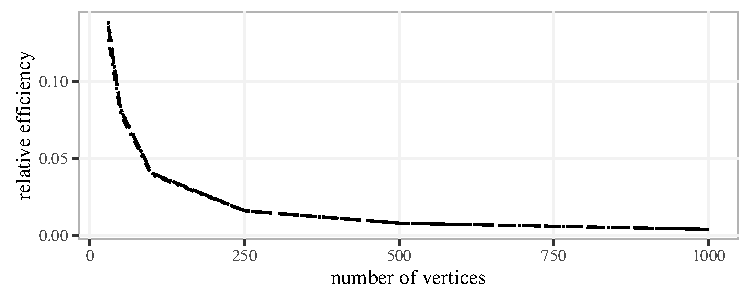
\includegraphics[width=1\textwidth]{./Figures/RE.pdf}
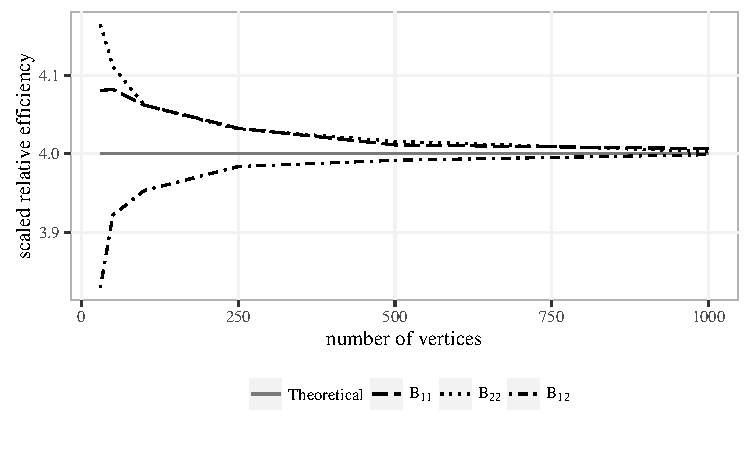
\includegraphics[width=1\textwidth]{./Figures/scaled_RE.pdf}
\caption[Finite sample relative efficiency based on simulations]{Finite sample relative efficiency based on simulations.
The top panel shows the estimated relative efficiency $\hat{\mathrm{RE}}(\bar{A},\hat{P})$ as a function of $n$ for fixed $m=100$ based on simulations of an SBM. 
For each value of $n$, we used 1000 Monte Carlo replicates of the SBM from Section~\ref{sec:sbm_sim} to estimate the RE.
Each curve corresponds to an average across vertex pairs corresponding to the three distinct block probabilities $B_{11}$, $B_{12}$, and $B_{22}$ in the two-block SBM.
Recall that values below 1 indicate that $\hat{P}$ is performing better than $\bar{A}$.
The relative efficiencies are all very close so the lines are indistinguishable. \\
To distinguish the three curves, the bottom panel shows the corresponding scaled relative efficiencies, $n \cdot \hat{\mathrm{RE}}(\bar{A},\hat{P})$.
The solid horizontal line indicates the theoretical asymptotic scaled relative which is  $1/\rho_s+1/\rho_t=4$, since $\rho_1=\rho_2=4$.
All the curves converge quickly to this theoretical limit. }
\label{fig:RE}
\end{figure}


Based on Theorem~\ref{thm:ARE}, we also have that the scaled RE converges to $1/\rho_{\tau_i}+1/\rho_{\tau_j}=4$ as $n \to\infty$ for all pairs $i,j$.
This is plotted as a solid line in the bottom panel.
From the figure, we see that $n \cdot \hat{\mathrm{RE}}_{st}(\bar{A}, \hat{P})$ converges to scaled asymptotic RE quite rapidly.
We omit error bars as the standard errors are very small for these estimates.

\begin{remark}
An intriguing aspect of these finite sample results is that the scaled relative efficiencies behave differently for small graphs with fewer vertices. 
The estimates of the edge probabilities for pairs of vertices in different blocks are much better than the estimates for edges within each block.
The reason for this is unclear and could be due to the actual values of the true probability, but it may also be due to the fact that there are approximately twice as many pairs of vertices in different blocks, $n^2/4$, than there are in the same block, $n^2/8-n/4$.
This could lead to an increase in effective sample size which may cause the larger differences displayed in the left parts of Figure~\ref{fig:RE}.
However, overall these differences are nearly indistinguishable for unscaled relative efficiency.
\end{remark}






\section{CoRR Brain Graphs Experiment}
\label{sec:LLG_corr_data}

In practice, graphs do not follow the independent edge model, let alone an RDPG or SBM, but the mean of a collection of graphs is still of interest for these cases.
To demonstrate that the estimator $\hat{P}$ is still useful in such cases, we tested its performance on structural connectomic data. 
The graphs are based on diffusion tensor MR images collected and available at the Consortium for Reliability and Reproducibility (CoRR) \citep{zuo2014open, gorgolewski2015high}.
The dataset contains 454 different brain scans, each of which was processed to yield an undirected, unweighted graph with no self-loops, using the pipeline described in \citet{roncal2013migraine} and \citet{kiar2016ndmg}.
The vertices of the graphs represent different regions in the brain defined according to an atlas.
We used three atlases, the JHU atlas with 48 vertices, the Desikan atlas with 70 vertices, and the  CPAC200 atlas with 200 vertices.
An edge exists between two vertices whenever there is at least one white-matter tract connecting the corresponding two regions of the brain. 
Details of this dataset are provided in the following section.


\subsection{Dataset Description}
\label{section:data}

The original dataset is from the Emotion and Creativity One Year Retest Dataset provided by Qiu, Zhang and Wei from Southwest University available at the Consortium for Reliability and Reproducibility (CoRR) \citep{zuo2014open, gorgolewski2015high}. It is comprised of 235 subjects, all of whom were college students. Each subject underwent two sessions of anatomical, resting state DTI scans, spaced one year apart. Due to incomplete data, only 454 scans are available.

When deriving MR connectomes, \citet{kiar2016ndmg} parcellate the brain into groups of voxels as defined by anatomical atlases. The atlases are defined either physiologically by neuroanatomists (Desikan and JHU), or are generated using an automated segmentation algorithm (CPAC200).
Once the voxels in the original image space are grouped into regions, an edge is placed between two regions when there is at least one white-matter tract, derived using a tractography algorithm, connecting the corresponding two parts of the brain.
The resulting graphs are undirected, unweighted, and have no self-loops.




\subsection{Experiment Results}

In order to evaluate the performance of the two estimators, we used a cross validation on the 454 graphs of each size. 
Specifically, for a given atlas, each Monte Carlo replicate corresponds to sampling $m$ graphs out of the 454 and computing the low-rank estimator $\hat{P}$ and the sample mean $\bar{A}$ using the $m$ selected graphs.
We then compared these estimates to the sample mean for the remaining $454-m$ adjacency matrices.
While we cannot interpret this mean graph as the probability matrix for an IEM distribution (see Section~\ref{sec:sim_iem}), the sample mean for the remaining graphs does give the proportion of times each pair of vertices are adjacent in the population from which the graphs were sampled.

While in previous sections we evaluated the mean squared error for either an individual entry or for an entire block in the SBM, in this section and the next section we will focus on the overall error for estimating the mean graph.
In particular we will use the average of the mean squared error across all pairs of vertices and we define $\mathrm{MSE}(\bar{A}) = \binom{n}{2}^{-1} \sum_{i<j}\Ex[\bar{A}_{ij}-P_{ij}]$ and similarly for $\mathrm{MSE}(\hat{P})$, which are also used for the relative efficiency.
As in the previous section, we will not use analytical evaluations of the MSE and instead estimate the MSE and relative efficiencies via Monte Carlo simulations.

We ran 1000 simulations on each of the three atlases for sample size $m=5, 10$. For $m=1$, we only have 454 different possibilities. So instead of running 1000 simulations, we looked through all 454 possible sample with size 1. As long as we determine which dimension to embed, the two estimates $\bar{A}$ and $\hat{P}$ can be calculated based on the sample.
In practice, we use algorithms like Zhu and Ghodsi's method or USVT discussed in Section~\ref{sec:dim_select} to select the dimension $d$. These methods are neither computationally advanced nor requiring sophisticated algorithms.
We plot the estimated relative efficiencies between $\bar{A}$ and $\hat{P}$ in Figure~\ref{fig:corr_re}.

\begin{figure}
\begin{center}
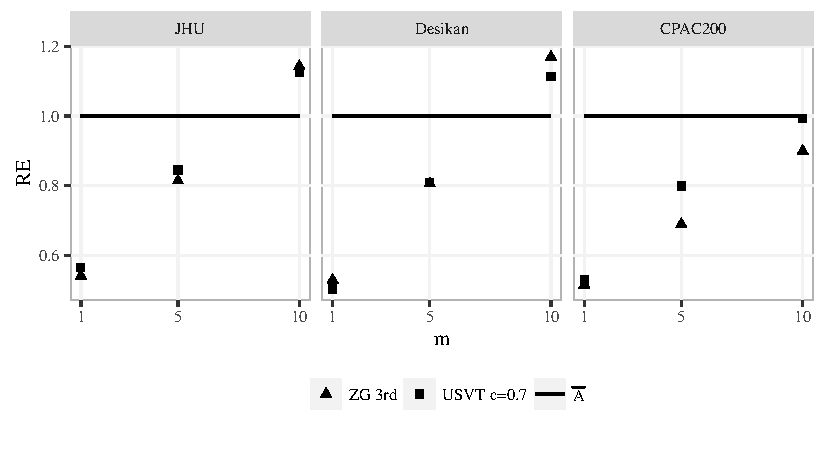
\includegraphics[width=1\linewidth]{./Figures/corr_data_REdiff.pdf}
\end{center}
\caption[Relative efficiencies of two estimators for the CoRR data set]{Relative efficiencies of $\bar{A}$ versus $\hat{P}$ for the CoRR data set.
For each atlas, JHU, Desikan, and CPAC 200, we sampled graphs which we used to compute $\bar{A}$ and $\hat{P}$.
We compared different sample sizes $m$ and different dimension selection procedures, ZG and USVT.
For each of the two methods for computing $\hat{P}$, we estimated their relative efficiencies with respect to the sample mean $\bar{A}$.
Confidence intervals all had lengths less than $0.015$, and hence we omitted them for clarity.
Overall, the relative efficiencies are greater for smaller sample sizes $m$ and larger number of vertices $n$.} 
\label{fig:corr_re}
\end{figure}

For each atlas and each sample size, we compare the Zhu and Ghodsi method \citep{zhu2006automatic} with the USVT method \citep{chatterjee2015matrix} and note that both perform reasonably well relative to the full-dimensional $\bar{A}$.
We omit confidence intervals for the estimated relative efficiencies since all confidence intervals have lengths less than $0.015$, indicating that all relative efficiencies, aside from the relative efficiency for the CPAC200 atlas at $m=10$, are very different from 1.

Again we can see that the largest improvements using $\hat{P}$ occur when $m$ is small and $n$ is large, where the RE are smaller than 1.
On the other hand, once $m=10$, $\bar{A}$ tends to do nearly as well or better than $\hat{P}$. 
Nonetheless, when applied to subgroups inference, such as all females between the age of 21 and 25, $\hat{P}$ can be really helpful for better exploring differences between groups compared to $\bar{A}$ due to a small sample size of each subgroup.
In addition, $\hat{P}$ offers certain advantages, especially since low-rank estimates can often be more easily interpretable by considering the latent position representation which will be discussed in Section~\ref{sec:interpretability}.

To further illustrate the differences between the two estimators, we considered a single random sample of size $m=5$ based on the Desikan atlas.
We calculated $\bar{A}$ and $\hat{P}$, using  Zhu and Ghodsi's 3rd elbow to select $d=11$. 
In Figure~\ref{fig:Matrix_desikan_m5}, the estimates $\bar{A}$ and $\hat{P}$ as well as the sample mean of 454 graphs (as a close estimate of $P$) are plotted in the upper level. 
Since the sample size is small, there are a lot of pairs of vertices with no edges or 5 edges in the 5 observations.
This leads to the white and black pixels in the image corresponding to $\bar{A}$.
On the other hand, $\hat{P}$ has a finer gradient of values which in this case leads to a more accurate estimate.
By calculating the mean squared error based on this sample, we can see that $\hat{P}$ (with mean squared error equals $0.015$) outperforms $\bar{A}$ (with mean squared error equals $0.016$), with a 3\% relative improvement.
In order to see where the improvements are clearly, in the upper triangular of the heat maps for $\bar{A}$ and $\hat{P}$, we highlight the edges (18 edges highlighted for $\bar{A}$ and 6 for $\hat{P}$) which have absolute estimation error larger than $0.4$.


Moreover, for the same sample discussed above, Figure~\ref{fig:Diff_desikan_m5} shows the values for the absolute estimation error $|\bar{A} - P|$ and $|\hat{P}-P|$. In addition, we include the absolute difference $|\bar{A} - \hat{P}|$ to show the overall difference between the two estimates. The lower triangular sections show the actual absolute difference while the upper triangular matrix highlights the vertex pairs with absolute differences larger than 0.4. 
There are 18 edges from $\bar{A}$ and 6 edges from $\hat{P}$ being highlighted in the figure, further indicating the superior performance of $\hat{P}$.
Note that approximately $13\%$ of all pairs of vertices are adjacent in all $454$ graphs and hence $\bar{A}$ will always have zero error for those pairs of vertices.
Nonetheless, $\hat{P}$ typically outperforms $\bar{A}$.

\begin{figure}
\begin{center}
  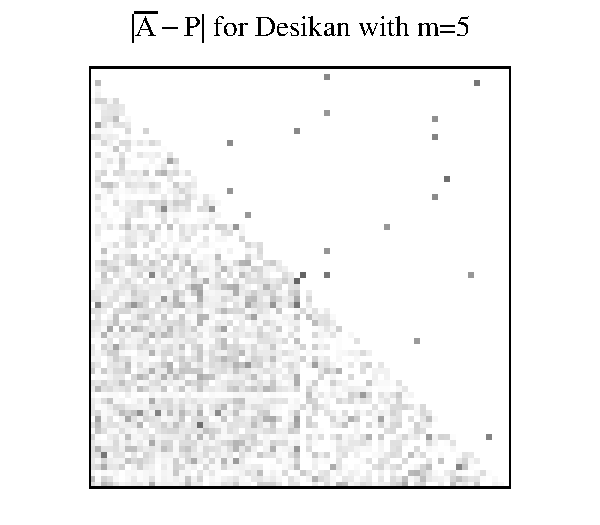
\includegraphics[height=.315\linewidth]{./Figures/Diff2_desikan_m5.pdf}\hspace{-40pt}
  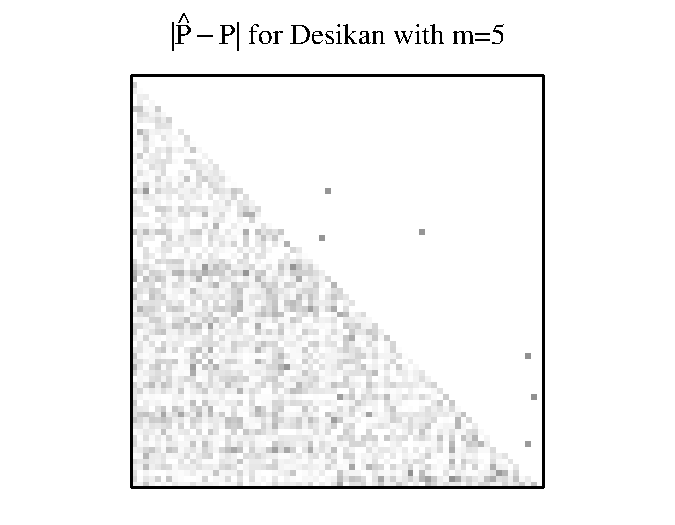
\includegraphics[height=.32\linewidth]{./Figures/Diff3_desikan_m5.pdf}\hspace{-34pt}
  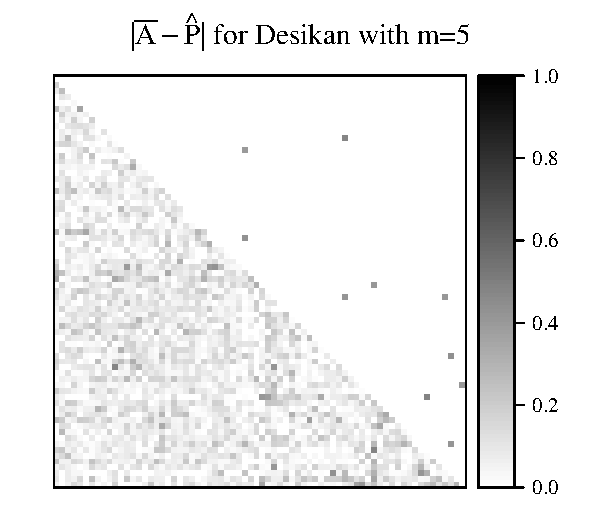
\includegraphics[height=.32\linewidth]{./Figures/Diff1_desikan_m5.pdf}
\end{center}
\caption[Heat plots of absolute estimation error for both estimators]{Heat plots of absolute estimation error for $\bar{A}$ and $\hat{P}$ (lower triangle) and absolute errors above 0.4 (upper triangle).
These heat plots show the absolute estimation error $|\bar{A} - P|$, $|\hat{P} - P|$ and $|\bar{A} - \hat{P}|$ for a sample of size $m=5$ from the Desikan dataset.
The embedding dimension for $\hat{P}$ is $d=11$ selected by the 3rd elbow of the ZG method. The lower triangular matrix shows the actual absolute difference, while the upper triangular matrix only highlights the edges with absolute differences larger than $0.4$. The fact that 18 edges from $\bar{A}$ are highlighted and only 6 edges from $\hat{P}$ are highlighted indicates that $\hat{P}$ has fewer large outliers compared to $\bar{A}$.
}
\label{fig:Diff_desikan_m5}
\end{figure}

To investigate the difference in performance with respect to the geometry of the brain, in Figure~\ref{fig:Diff_between_desikan} we plot the 50 edges with the largest differences $|\bar{A}_{ij} - P_{ij}| - |\hat{P}_{ij} - P_{ij}|$ according to the location of the corresponding regions in the brain. Red edges indicate that $\hat{P}$ overestimates $P$, while blue means that $\hat{P}$ underestimates $P$. The edge width is determined by the estimation error for $\hat{P}$, where pairs with larger estimation error are represented by thicker lines.
We also highlight the five regions corresponding to vertices that contribute most to the difference, meaning the vertices $i$ with the largest value of $\sum_j (|\bar{A}_{ij} - P_{ij}| - |\hat{P}_{ij} - P_{ij}|)$.
Notably, three of these top five regions form a contiguous group of regions.
The top five regions are the inferior temporal, middle temporal, and transverse temporal regions in the left hemisphere and the parahippocampal and parsopercularis regions in the right hemisphere of the Desikan atlas.

\begin{figure}[!htbp]
\centering
\includegraphics[width=1\textwidth]{./Figures/Diff_between_desikan.png}
\caption[Top 5 regions of the brain and top 50 connections between regions with the largest differences between two estimators]{Top 5 regions of the brain (vertices in graphs) and top 50 connections between regions (edges in graphs) with the largest differences $|\bar{A}_{ij} - P_{ij}| - |\hat{P}_{ij} - P_{ij}|$.
Red edges indicate that $\hat{P}$ overestimate $P$ while blue means that $\hat{P}$ underestimates $P$. The edge width is determined by the estimation error. Connections with larger estimation error are represented by thicker lines. This figure shows the regions and connections of the brain where $\hat{P}$ outperforms $\bar{A}$ the most for estimating $P$.}
\label{fig:Diff_between_desikan}
\end{figure}

\subsection{Exploration of Dimension Selection Procedures}

To further investigate the impact of the dimension selection procedures, we also considered all possible dimensions for $\hat{P}$ by ranging $d$ from 1 to $n$ in order to investigate the impact of the dimension selection procedures.
We plot $\hat{\mathrm{MSE}}$ of $\bar{A}$ and $\hat{P}$ in Figure~\ref{fig:LLG_realdata_MSE}.
The horizontal axis gives dimension $d$, which only impacts $\hat{P}$, which is why estimated MSE of $\bar{A}$ is shown as flat.

When $d$ is small, $\hat{P}$ underestimates the dimension and throws away important information, which leads to relatively poor performance. When $d=n$, $\hat{P}$ is equal to $\bar{A}$, so that the curve for $\hat{\mathrm{MSE}}$ for $\hat{P}$ ends at $\hat{\mathrm{MSE}}(\bar{A})$. 

In the figure, we denote the 3rd elbow found by the Zhu and Ghodsi method by a triangle, and denote the dimension selected by USVT with threshold 0.7 by a square. 
% (with largest 95\% confidence interval length to be $3.5$)
% (with largest 95\% confidence interval length to be $0.7$) 
Both dimension selection algorithms tend to select dimensions which nearly minimize the mean squared error.
% The standard error for the Zhu and Ghodsi and the USVT methods are about $0.9$ and $0.17$ respectively.

When $m$ is 1 or 5, $\bar{A}$ has large variance which leads to large $\hat{\mathrm{MSE}}$. Meanwhile, $\hat{P}$ reduces the variance by taking advantages of inherent low-rank structure of the mean graph. Such smoothing effect is especially obvious while we only have 1 observation. When $m = 1$, all weights of the graph are either 0 or 1, leading to a very bumpy estimate $\bar{A}$. In this case, $\hat{P}$ smooths the connectomes estimate and improves the performance.
Additionally, we see that there is a large range of dimensions where the performance for $\hat{P}$ is superior to $\bar{A}$. 
With a larger $m$, the performance of $\bar{A}$ improves so that its performance is frequently superior but nearly identical to $\hat{P}$.

\begin{figure}[!htbp]
\centering
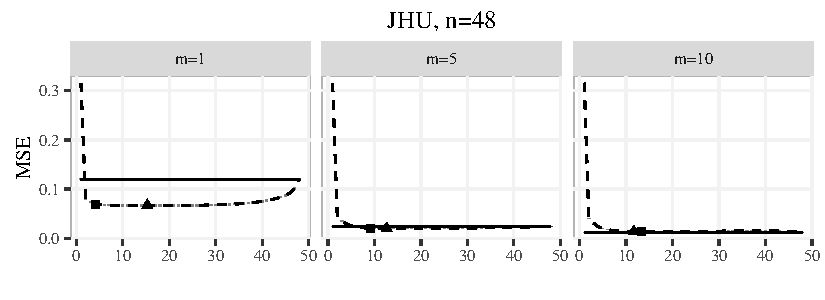
\includegraphics[width=.99\textwidth]{./Figures/corr_data_MSE_jhu.pdf}\\
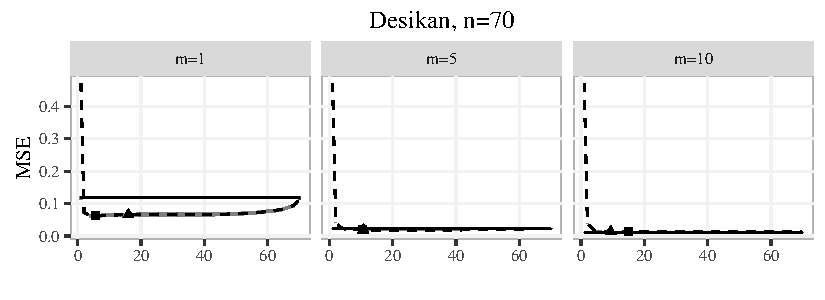
\includegraphics[width=.99\textwidth]{./Figures/corr_data_MSE_desikan.pdf}\\
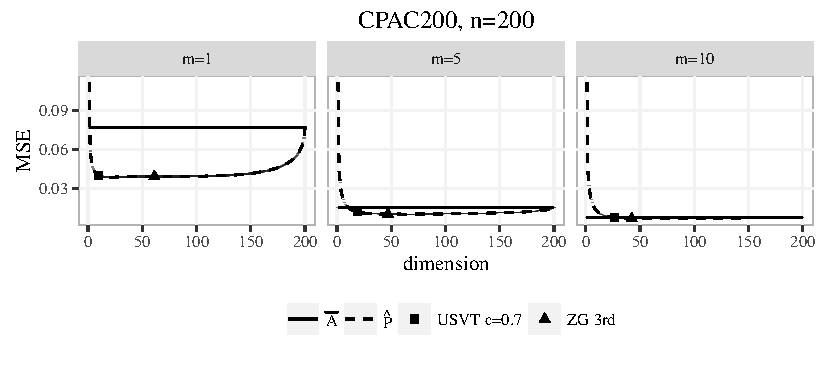
\includegraphics[width=.99\textwidth]{./Figures/corr_data_MSE_CPAC200.pdf}
\caption[Comparison of MSE of two estimators for three atlases at three sample sizes for the CoRR data]{Comparison of $\hat{\mathrm{MSE}}$ of $\hat{P}$ and $\bar{A}$ for three atlases at three sample sizes for the CoRR data.
These plots show the MSE for $\bar{A}$ (solid line) and $\hat{P}$ (dashed line) for three dataset (JHU, Desikan, and CPAC200) while embedding the graphs into different dimensions and with different sample sizes $m$. The average dimensions chosen by the 3rd elbow of Zhu and Ghodsi is denoted by a triangle
 and those chosen by USVT with threshold equaling 0.7 is denoted by a square.
Vertical intervals, visible mainly in the $n=48,70$ and $m=1$ plots, represent the 95\% confidence interval for the mean squared errors. }
\label{fig:LLG_realdata_MSE}
\end{figure}


\subsection{Interpretability of Low-rank Methods}
\label{sec:interpretability}

Low-rank methods can often be more easily interpreted in a vertexy way.
In particular, in the RDPG model, by representing a low-rank matrix in terms of the latent positions, where each vertex is represented as a vector in $\mathbb{R}^d$ and the entries of the matrix are given by the inner products of these vectors, one can analyze and visualize the geometry of these vectors in order to interpret how each vertex is behaving in the context of the larger graph. 
Now we take the CoRR brain graphs with Desikan atlases as an example. By embedding the mean graph $P$ which is the average of all 454 graphs, we get the estimated latent positions $\hat{X} \in \mathbb{R}^{n \times d}$, where $n=70$ is the number of vertices and $d = 8$ is the dimension selected by the Zhu and Ghodsi's method.
We color the brain using the first 4 dimensions of $\hat{X}$ as in Figure~\ref{fig:eigenvector_brain} respectively. By the figure of the second dimension, we can see a clear distinction of the left and right hemisphere as conveyed in the second dimension. Additionally, such a representation allows the use of techniques from multivariate analysis to further study the estimated population mean.

\begin{figure}	
\centering
\begin{subfigure}[t]{.7\textwidth}
\caption{1st dimension}
\vspace*{-16pt}
\begin{center}
  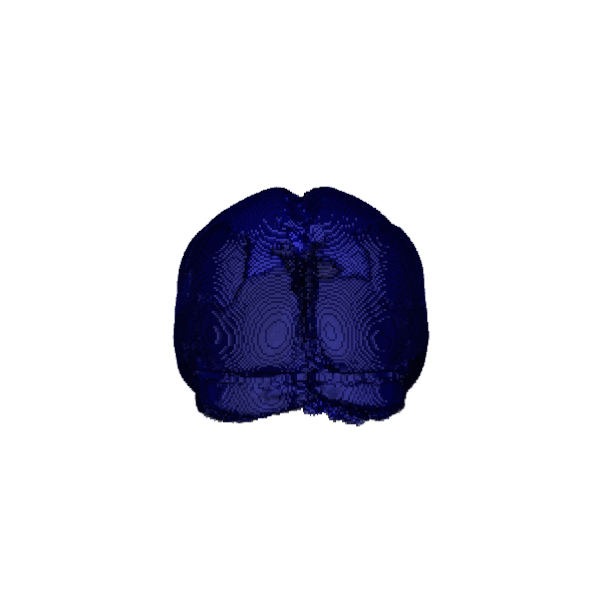
\includegraphics[trim={5cm 5cm  4cm  4cm },clip,height=.34\linewidth]{./Figures/desikan1a.png}\hspace{-9pt}
  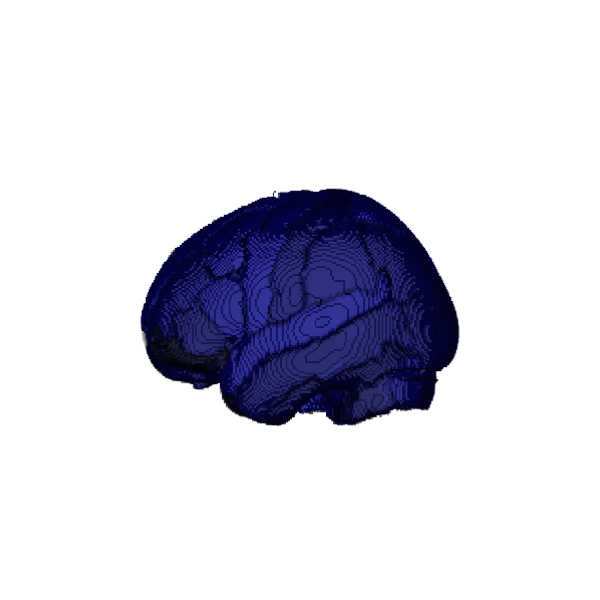
\includegraphics[trim={5cm 5cm  4cm  4cm },clip,height=.34\linewidth]{./Figures/desikan1b.png}\hspace{-9pt}
  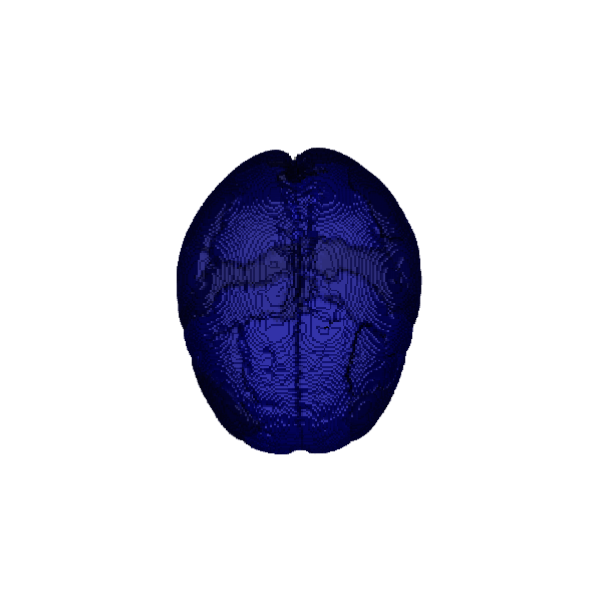
\includegraphics[trim={5cm 5cm  4cm  4cm },clip,height=.34\linewidth]{./Figures/desikan1c.png}
\end{center}
\end{subfigure}\\
\vspace*{5pt}
\begin{subfigure}[t]{.7\textwidth}
\caption{2nd dimension}
\vspace*{-16pt}
\begin{center}
  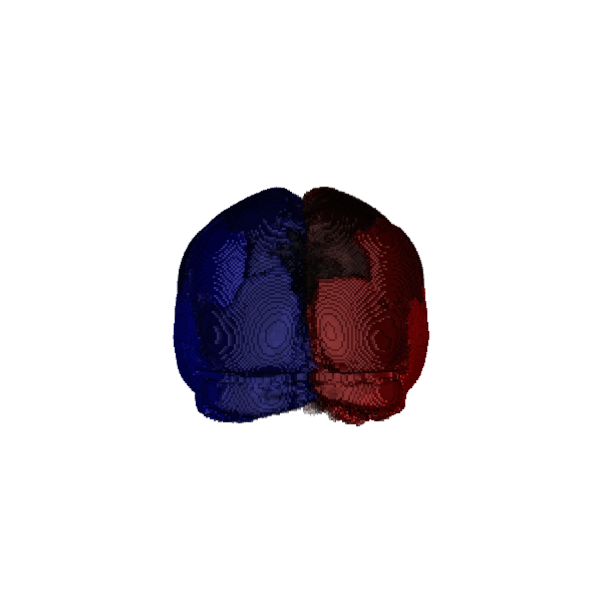
\includegraphics[trim={5cm 5cm  4cm  4cm },clip,height=.34\linewidth]{./Figures/desikan2a.png}\hspace{-10pt}
  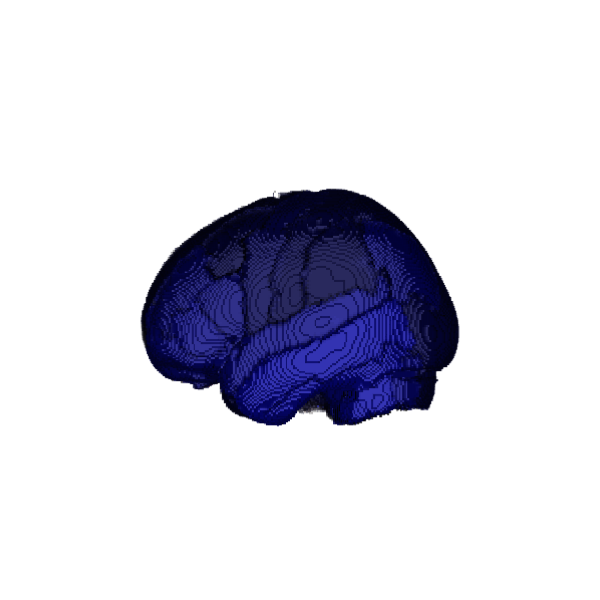
\includegraphics[trim={5cm 5cm  4cm  4cm },clip,height=.34\linewidth]{./Figures/desikan2b.png}\hspace{-10pt}
  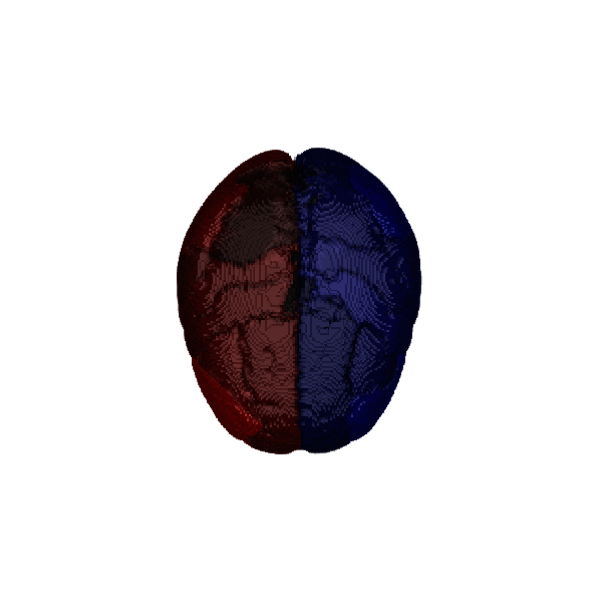
\includegraphics[trim={5cm 5cm  4cm  4cm },clip,height=.34\linewidth]{./Figures/desikan2c.png}
\end{center}
\end{subfigure}\\
\vspace*{5pt}
\begin{subfigure}[t]{.7\textwidth}
\caption{3rd dimension}
\vspace*{-16pt}
\begin{center}
  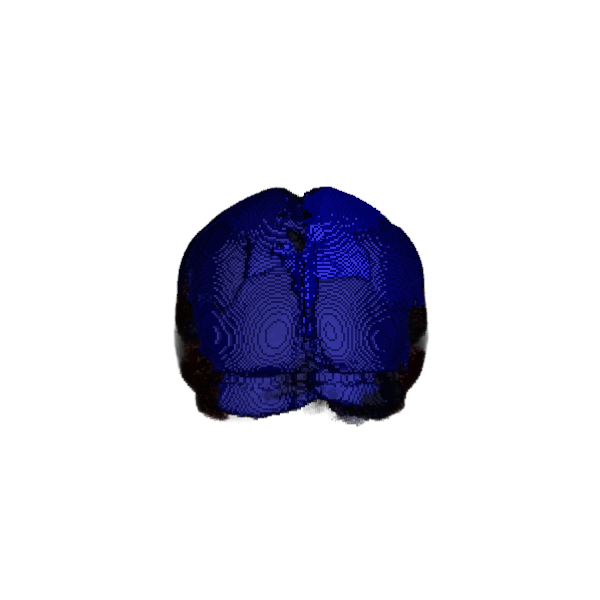
\includegraphics[trim={5cm 5cm  4cm  4cm },clip,height=.34\linewidth]{./Figures/desikan3a.png}\hspace{-10pt}
  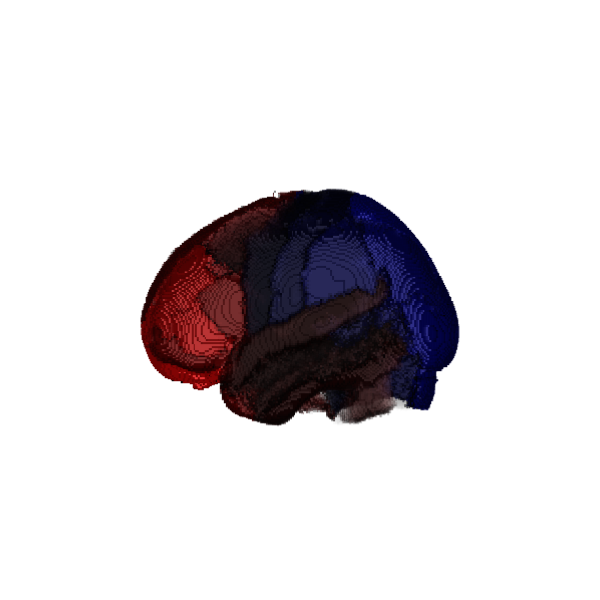
\includegraphics[trim={5cm 5cm  4cm  4cm },clip,height=.34\linewidth]{./Figures/desikan3b.png}\hspace{-10pt}
  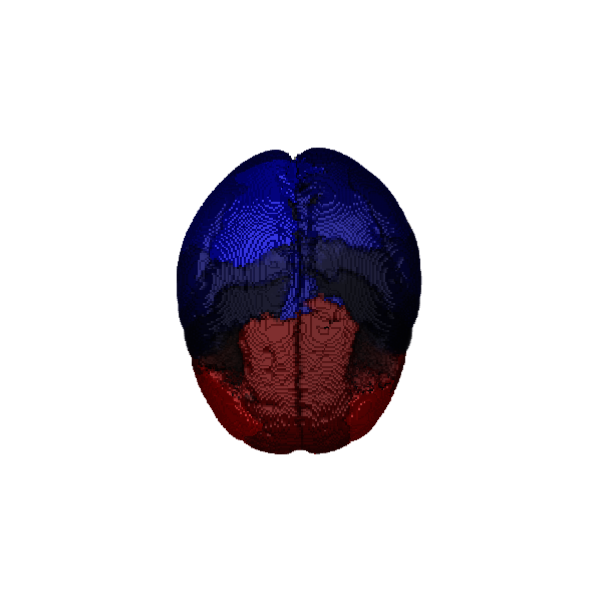
\includegraphics[trim={5cm 5cm  4cm  4cm },clip,height=.34\linewidth]{./Figures/desikan3c.png}
\end{center}
\end{subfigure}\\
\vspace*{5pt}
\begin{subfigure}[t]{.7\textwidth}
\caption{4th dimension}
\vspace*{-16pt}
\begin{center}
  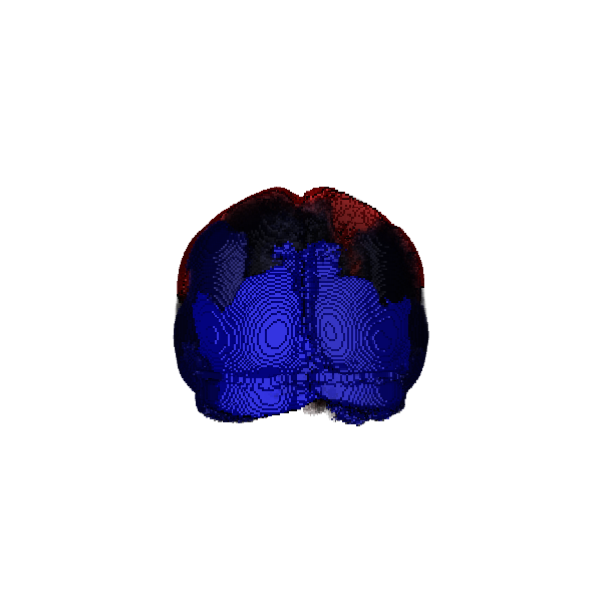
\includegraphics[trim={5cm 5cm  4cm  4cm },clip,height=.34\linewidth]{./Figures/desikan4a.png}\hspace{-10pt}
  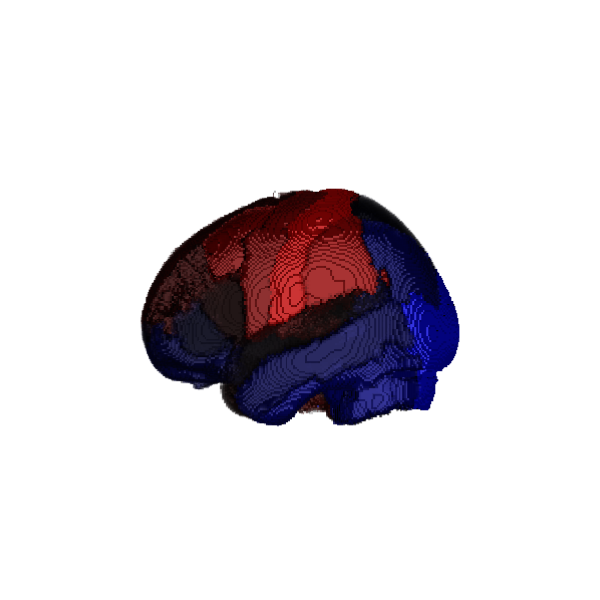
\includegraphics[trim={5cm 5cm  4cm  4cm },clip,height=.34\linewidth]{./Figures/desikan4b.png}\hspace{-10pt}
  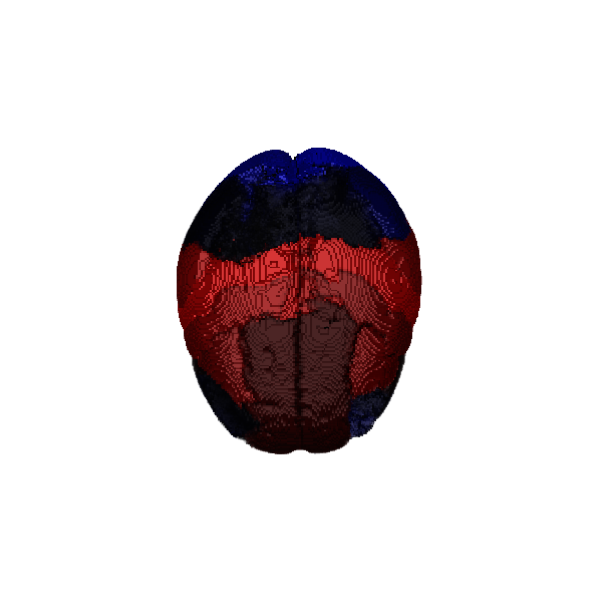
\includegraphics[trim={5cm 5cm  4cm  4cm },clip,height=.34\linewidth]{./Figures/desikan4c.png}
\end{center}
\end{subfigure}\\
\caption[Brain plots colored by the first 4 dimensions of embedding for the Desikan atlas]{Brain plots colored by the first 4 dimensions of $\hat{X}$ for the Desikan atlas respectively.
We plot the brain using the first 4 dimensions of $\hat{X}$. From the figure, we can see the embeddings have their own neuro-meaning, for example there is a clear distinction of the left and right hemisphere as conveyed in the second dimension. Also, the first dimension provides an average level of the entire brain.}
\label{fig:eigenvector_brain}
\end{figure}



\subsection{Challenges of the CoRR Dataset}

While our estimator $\hat{P}$ performs well when the sample size $m$ is small and the number of vertices $n$ is large, the CoRR dataset itself does not strictly adhere to the low-rank assumptions of our theory.

As discussed in Remark \ref{remark:low_rank}, we first check whether the dataset has the low-rank property or not. In Figure~\ref{fig:LLG_screeplot}, we plot the relative error $\|\mathrm{lowrank}_d(P)-P\|_F^2/\|P\|_F^2$ of using a rank-$d$ approximation of $P$ (see Algorithm~\ref{algo:LLG_lowrank}) as solid curves.
The rate at which this curve tends to zero provides an indication of the relative performance of using $\hat{P}_d$ as compared to $\bar{A}$ when $m$ is large. 
For all three atlases, while these error rates do tend to zero relatively quickly, substantial errors remain for any low-rank approximation.
This can be compared to the dashed lines which show how these errors would behave if $P$ was truly low-rank.
As can be expected, the CoRR dataset is actually high-rank, which violates the low-rank assumption.

\begin{figure}[!htbp]
\centering
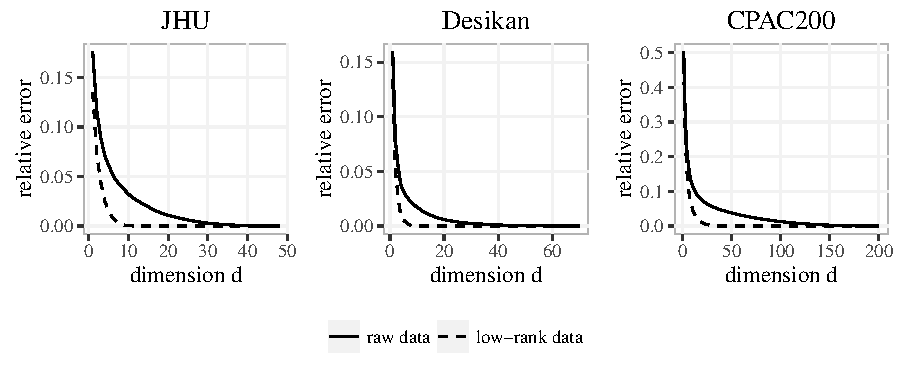
\includegraphics[width=.6\textheight]{./Figures/screeplot_ratio_all.pdf} 
\caption[Relative error of the low-rank approximation of the population mean]{Relative error of the rank-$d$ approximation of the population mean.
The solid curves show the relative error $\|\mathrm{lowrank}_d(P)-P\|_F^2/\|P\|_F^2$ of using a rank-$d$ approximation of $P$ (see Algorithm~\ref{algo:LLG_lowrank}) for three different atlases.
The relative error decays relatively slowly when $d$ is close to $n$, which indicates that $P$ is not low-rank.
Also, if $P$ actually has the low-rank property, the relative error plot will look like the dashed curves, where we revised $P$ to be low-rank by only keeping a few large eigenvalues. }
\label{fig:LLG_screeplot}
\end{figure}

In addition, by plotting the histograms of the eigenvalues of $P$ in Figure~\ref{fig:LLG_histogram}, we see that there are a bunch of negative eigenvalues, which indicates that the positive semi-definiteness is also violated in this real data experiment. This makes it even harder for $\hat{P}$ to outperform $\bar{A}$. 

 \begin{figure}[!htbp]
 \centering
 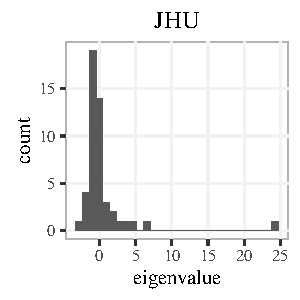
\includegraphics[height=.2\textheight]{./Figures/hist_JHU.pdf} 
 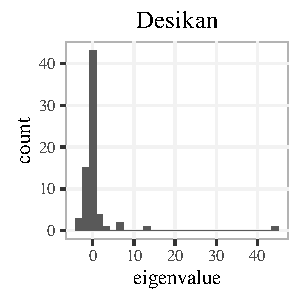
\includegraphics[height=.2\textheight]{./Figures/hist_desikan.pdf} 
 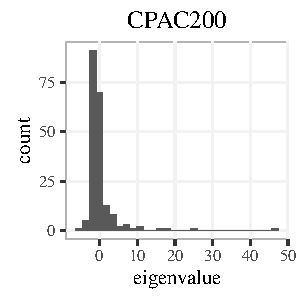
\includegraphics[height=.2\textheight]{./Figures/hist_CPAC200.pdf}
 \caption[Histogram of the population mean]{Histogram of the population mean.
 These figures show the histograms of the eigenvalues of the mean graph of all 454 graphs with diagonal augmentation. A bunch of negative eigenvalues indicate that $P$ is not positive semi-definite.
 }
 \label{fig:LLG_histogram}
 \end{figure}


Two other parts of this dataset provide challenges for our low-rank methods.
First, there are a large number of negative eigenvalues which $\hat{P}$ will not capture.
We can adapt our low-rank methods by including large negative eigenvalues as well however we found that for low sample sizes excluding negative eigenvalues improved performance.
Second, approximately 12.8\% of the entries of $P$ are exactly equal to 1.
For these edges, $\bar{A}$ will always have zero error, while $\hat{P}$ will necessarily give a less accurate estimate. 

Moreover, by the histogram of $P$, i.e. the entry-wise mean of all 454 graphs based on the Desikan atlas, as in Figure~\ref{fig:P_hist_desikan}, we can clearly see more edge probabilities are concentrated on both sides, i.e. close to 0 or 1. In particular, 12.8\% of the edges has probability equals to 1 exactly. For these edges, MLE $\bar{A}$ always recover the probability 1 exactly even with only 1 observation, while $\hat{P}$ will give a less accurate estimate because of the smoothing effect. So the CoRR dataset we consider is highly preferable to $\bar{A}$ compared to $\hat{P}$. 
However, even in this situation, $\hat{P}$ still outperforms $\bar{A}$ when the sample size is relatively small.

 \begin{figure}[!htbp]
 \centering
 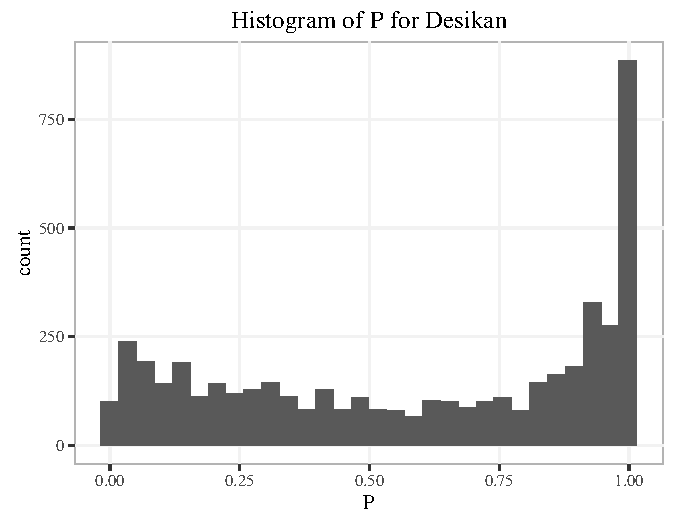
\includegraphics[width=0.8\textwidth]{./Figures/P_hist_desikan.pdf}
 \caption[Histogram of mean graph for Desikan atlas]{Histogram of $P$ for Desikan atlas.
 This figure shows the histogram of $P$, i.e. the entry-wise mean of all 454 graphs based on the Desikan atlas. More edge probabilities of $P$ are concentrated on both sides, i.e. close to 0 or 1. In particular, 12.8\% of the edges has probability equals to 1 exactly.}
 \label{fig:P_hist_desikan}
 \end{figure}

Despite all these challenges, our results show that when the sample size is relatively small, such as $m=1$ or $m=5$, and for the atlases with a larger number of vertices, $\hat{P}$ still gives a better estimate than $\bar{A}$ for the CoRR dataset.
Importantly, this improvement is robust to the embedding dimension provided the dimension is not underestimated.



\subsection{Lobe Structure behind the Low-rank Methods}
\label{section:lobe_structure}
In previous sections, we have shown that how the low-rank methods help us improve the accuracy of estimation while providing convenient interpretations simultaneously. Certainly there is more behind it. In this section, we focus on the lobe structure in particular.

The lobes of the brain is an anatomical classification, which has been shown to be related to different brain functions. Basically, there are 4 different lobes for each hemisphere, i.e. Frontal, Parietal, Occipital, and Temporal.
For the Desikan atlas, there are 70 different regions (35 regions for each hemisphere). Each region belongs to one lobe. However, 8 regions of the Desikan atlas (Unknown, Banks of Superior Temporal Sulcus, and Corpus Callosum, for both hemispheres) do not have obvious lobe assignment. So we cluster them into a new lobe category named ``other'' to resolve this issue.

Generally, the regions within the same lobe should be more similar compared to the regions across the lobes. In order to see whether the embedded latent positions $X$ preserve this property or not, we propose a test statistics $T$ to be the average differences between vertices within the same lobe minus the average differences between vertices across different lobes, i.e.
\[
T(X, l) = \frac{\sum_{i \ne j, l(i) = l(j)} \|X_i - X_j \|_2}{\sum_{i \ne j, l(i) = l(j)} 1} -
\frac{\sum_{i \ne j, l(i) \ne l(j)} \|X_i - X_j \|_2}{\sum_{i \ne j, l(i) \ne l(j)} 1},
\]
where $l(i)$ represents the lobe assignment for vertex $i$. If the latent positions $X$ and the lobe assignment $l$ are independent, then we expect $T(X, l)$ to be close to zero. A small test statistic $T(X, l)$ indicates that latent positions of the regions within the same lobe are closer compared to the ones across the lobes, which is evidence that the low-rank methods preserves the lobe structure.

However, the anatomical geometry might contribute to the dependence between $X$ and $l$ and we do not want to be distracted by this factor. So instead of testing the dependence between $X$ and $l$, we are more interested in the following hypothesis test:

$H_0$: $X$ and $l$ are conditionally independent given anatomical geometry.

$H_A$: $X$ and $l$ are conditionally dependent given anatomical geometry.

In this situation, we can focus on how much of the lobe structure is really captured by the low-rank methods without affected by the inherent spatial relationship. Note that this test is significantly underpowered compared to the test on a unconditional independence.
To test under the anatomical geometry conditions, we permute the lobe assignment $l$ in a way that the number of regions in each lobe remain the same and the regions within the same lobe are still spatially connected. In order to permute under such constraints, we define a flip to be a swap of two pairs of vertices which keeps the number of regions in each lobe, and do it several times.

As mentioned before, there are 10 lobes and 70 regions based on the Desikan atlas. 
We say two regions are adjacent if they share a common boundary. We denote such spatial adjacency by an adjacency matrix $S$ for the 70 regions, where $S_{ij} = 1$ means region $i$ and region $j$ are contain a pair of voxels, $v_i$ and $v_j$, which are spatially adjacent.
If this is true, then we say region $j$ is a neighbor of region $i$.
We denote the lobe i.d. for region $i$ by $l_i$.

Now we define a uniform $1$-flip to be:
\begin{enumerate}
\item Select a pair of adjacent regions (region $i_1$ and region $j_1$) across the boundary of lobes uniformly, i.e. $S_{i_1 j_1} = 1$ and $l(i_1) \ne l(j_1)$;
\item Uniformly select another pair of adjacent regions (region $i_2$ and region $j_2$ where $i_1 \ne i_2$ and $j_1 \ne j_2$) across the same boundary of lobes uniformly, i.e. $S_{i_2 j_2} = 1$ and $l(i_1) = l(i_2)$ and $l(j_1) = l(j_2)$;
\item Reassign region $j_1$ to lobe $l_{i_1}$ and reassign region $i_2$ to lobe $l_{j_2}$.
\end{enumerate}

By the definition, after a uniform $1$-flip, the number of regions in each lobe stays the same, where only two regions are changed to a different lobe.

Then we can define a uniform $k$-flip naturally as sequentially performing uniform $1$-flip $k$ times.
Note that after a uniform $k$-flip, the number of regions in each lobe still keeps the same.

In the permutation test, we apply a uniform $k$-flip and calculate the test statistic $T(X, l)$ based on the lobe assignment after flipping.
The $p$-value is computed as the proportion of uniform $k$-flips with a $T$ value smaller than the $T$ value for the true lobe assignments.


For a fixed number of flips, we ran 1000 simulations and calculate the test statistics $T(X, l)$ after the permutation. We vary the number of flips from 1 to 10 and the results are shown in Figure~\ref{fig:violin_plot}. In this violin plot, we use dashed line to represent the $T(X, l)$ based on the true lobe assignment. As the number of flips increases, $T(X, l)$ converges to the expected value under the assumption that $X$ and $l$ are independent in a constrained way mentioned above. And we can see that the $T(X, l)$ according to the true lobe assignment move away from the 95\% confidence interval. We also calculate the corresponding p-values and labeled them in the figure. We can see that when the number of flips is larger than 7, the p-value is less than 0.05, which suggests that the latent positions based on the low-rank methods preserves the lobe structure regardless of the anatomical geometry.

\begin{figure}[!htbp]
\centering
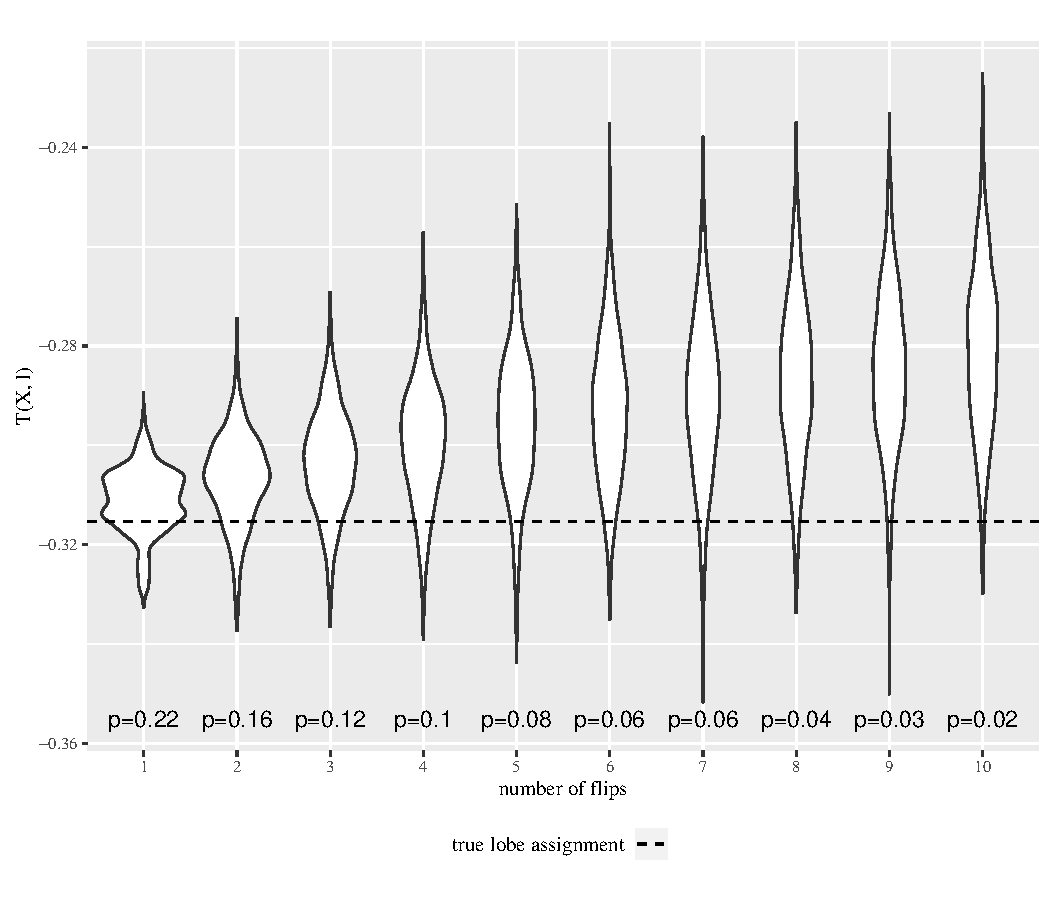
\includegraphics[width=1\textwidth]{./Figures/violinplot_new_flip_2norm_1_8.pdf}
\caption[Violin plot of the permutation test]{Violin plot of the permutation test.
We run 1000 simulations for each number of flips. Dashed line represents the situation based on true lobe assignment. As the number of flips increases, $T(X, l)$ converges to the expected value under the assumption that $X$ and $l$ are independent in a constrained way mentioned above. And we can see that the $T(X, l)$ according to the true lobe assignment move away from the 95\% confidence interval.}
\label{fig:violin_plot}
\end{figure}

%\begin{figure}[!htbp]
%\centering
%\includegraphics[width=0.8\textwidth]{pvalue_new_flip_2norm_1_8.pdf}
%\caption{{\bf P-value of the permutation test.}
%This figure shows the p-value of the permutation test based on different number of flips. When the number of flips is larger than 7, the p-value is less than 0.5, which suggests that the latent positions based on the low-rank methods preserves the lobe structure.}
%\label{fig:pvalue}
%\end{figure}





%\begin{figure}[!htbp]
%\centering
%\includegraphics[width=1\textwidth]{JHU.png}
%\caption{Comparison of MSE between $\bar{A}$ (solid line) and $\hat{P}$ (dashed line) for JHU dataset while embedding the graphs into different dimensions with different size $M$ of the subsamples. The dimension chosen by the 3rd elbow of Zhu and Ghodsi is denoted in triangle, and chosen by USVT with threshold equals 0.7 is denoted in square. Vertical intervals represent the 95\% confidence interval. When $M$ is small, $\hat{P}$ outperforms $\bar{A}$ with a flexible range of the embedding dimension including what Zhu and Ghodsi selects.}
%\label{fig:JHU}
%\end{figure}
%
%\begin{figure}[!htbp]
%\centering
%\includegraphics[width=1\textwidth]{desikan.png}
%\caption{Comparison of MSE between $\bar{A}$ (solid line) and $\hat{P}$ (dashed line) for desikan dataset while embedding the graphs into different dimensions with different size $M$ of the subsamples. The dimension chosen by the 3rd elbow of Zhu and Ghodsi is denoted in triangle, and chosen by USVT with threshold equals 0.7 is denoted in square.  Vertical intervals represent the 95\% confidence interval.  When $M$ is small, $\hat{P}$ outperforms $\bar{A}$ with a flexible range of the embedding dimension including what Zhu and Ghodsi selects.}
%\label{fig:desikan}
%\end{figure}
%
%\begin{figure}[!htbp]
%\centering
%\includegraphics[width=1\textwidth]{CPAC200.png}
%\caption{Comparison of MSE between $\bar{A}$ (solid line) and $\hat{P}$ (dashed line) for CPAC200 dataset while embedding the graphs into different dimensions with different size $M$ of the subsamples. The dimension chosen by the 3rd elbow of Zhu and Ghodsi is denoted in triangle, and chosen by USVT with threshold equals 0.7 is denoted in square.  Vertical intervals represent the 95\% confidence interval.  When $M$ is small, $\hat{P}$ outperforms $\bar{A}$ with a flexible range of the embedding dimension including what Zhu and Ghodsi selects.}
%\label{fig:CPAC200}
%\end{figure}
%
%\begin{figure}
%\centering
%\begin{subfigure}{.33\textwidth}
%  \centering
%  \includegraphics[width=1.2\linewidth]{P_JHU.png}
%\end{subfigure}%
%\begin{subfigure}{.33\textwidth}
%  \centering
%  \includegraphics[width=1.2\linewidth]{Abar_JHU_m5.png}
%\end{subfigure}
%\begin{subfigure}{.33\textwidth}
%  \centering
%  \includegraphics[width=1.2\linewidth]{Phat_JHU_m5.png}
%\end{subfigure}
%\caption{Comparison between the mean of 454 graphs $P$ and two estimates $\bar{A}$ and $\hat{P}$ derived from a sample of size $M=5$ from JHU dataset while embedding the graphs into dimension $d=15$ selected by the 3rd elbow of ZG method.}
%\label{fig:adj_JHU_m5}
%\end{figure}
%
%\begin{figure}[!htbp]
%\centering
%\includegraphics[width=1\textwidth]{Vertex_Diff_Phat_desikan.png}
%\caption{Top 5 regions of the brain (vertices in graphs) with largest absolute difference $|\hat{P} - P|$.}
%\label{fig:Vertex_Diff_Phat_desikan}
%\end{figure}
%
%\begin{figure}[!htbp]
%\centering
%\includegraphics[width=1\textwidth]{Edge_Diff_Phat_desikan.png}
%\caption{Top 1\% (49) connections between regions (edges in graphs) with largest absolute difference $|\hat{P} - P|$.}
%\label{fig:Vertex_Diff_Phat_desikan}
%\end{figure}








\section{Synthetic Data Analysis for Full Rank IEM}
\label{sec:sim_iem}

While the theory we have developed is based on the assumption that the mean graph is low rank, as we have seen in Section~\ref{sec:LLG_corr_data}, $\hat{P}$ often performs well even when this assumption is false. 
To further illuminate this point, we performed a synthetic data analysis under a full-rank independent edge model where we used the sample mean of the 454 graphs in the Desikan dataset as the probability matrix $P$.
As in the previous section, we simulated datasets from the full rank IEM distribution with probability matrix $P$ of size $m=1,5$, and $10$ and used $\bar{A}$ and $\hat{P}$, where we varied the rank of $\hat{P}$ from $1$ to $70$.

Figure~\ref{fig:sim_desikan} shows the resulting estimated MSE for $\bar{A}$ (solid line) and $\hat{P}$ (dashed line) for simulated data based on the full rank probability matrix $P$ shown in the left panel of Figure~\ref{fig:Matrix_desikan_m5}.
We see that the results are very similar to those presented in Section~\ref{sec:LLG_corr_data}, though overall $\hat{P}$ performs even better than in the real data experiments. 
When $m$ is small, $\hat{P}$ outperforms $\bar{A}$ with a flexible range of the embedding dimension including those selected by the Zhu and Ghodsi method.
On the other hand, when $m$ is large enough, both estimators perform well with the decision between the two being less conclusive.
This simulation again shows the robustness of $\hat{P}$ to deviations from the RDPG model, specifically if the probability matrix is full-rank.

We also note that the finite-sample relative efficiency in these cases shows is even more favorable to $\hat{P}$, with relative efficiencies lower than $1/3$ for $m=1$, than for the real data, where relative efficiencies were at best around $1/2$ for $m=1$.
From this observation, we can postulate that the degradation in the performance of $\hat{P}$ in real data can at least partially be attributed to the fact that the independent edge assumption does not hold for real data.


\begin{figure}[!htbp]
\centering
\includegraphics[width=1\textwidth]{./Figures/sim_desikan.pdf}
\caption[Comparison of two estimators for synthetic data analysis]{Comparison of $\hat{P}$ and $\bar{A}$ for synthetic data analysis.
As in Figure~\ref{fig:RE}, this figure shows $\hat{\mathrm{MSE}}$ for $\bar{A}$ (solid line) and $\hat{P}$ (dashed line) for simulated data with different sample sizes $m$ based on the sample mean for the Desikan dataset. Again, the average of dimensions selected by the USVT method (square) and the ZG method (triangle) tend to nearly approximate the optimal dimension. 
Overall, we see that the structure of these plots well approximates the structure for the real data indicating that performance for the independent edge model will tend to translate in structure to non-independent edge scenarios. 
On the other hand, the relative efficiency $\hat{\mathrm{RE}}(\bar{A},\hat{P})$ is lower for this synthetic data analysis than for the CoRR data.}
\label{fig:sim_desikan}
\end{figure}




%\section{Discussion}
%\label{sec:LLG_discussion}
%
%Motivated by the RDPG model, in this chapter, our methodology takes advantage of the low-rank structure of the graphs by applying low-rank approximation to the entry-wise MLE. 
%We give a closed form for the asymptotic relative efficiency between the entry-wise MLE $\bar{A}$ and our estimator $\hat{P}$ in the case of a stochastic blockmodel, demonstrating that when the number of vertices $N$ is sufficiently large, low-rank methods provide a substantial improvement.
%In particular, we show that for a stochastic blockmodel with fixed number of blocks $K$, block size proportion $\rho$, and number of graphs $m$, the low-rank estimator $\hat{P}$ has MSE which is on the order of $n$ times lower than the MSE for $\bar{A}$.
%
%Moreover, our estimator outperforms the entry-wise MLE in a cross validation analysis of the CoRR brain graphs and in low- and full-rank simulation settings.
%These results illustrate that $\hat{P}$ performs well even when the low-rank assumption is violated and that $\hat{P}$ is robust and can be applied in practice.
%
%One of the key observations from our real data analysis was that the largest improvements using the low-rank method occurred when the number of graphs $m$ was small, and that it provided only minor improvements or even degraded performance slightly when $m$ was large. 
%However, even in large scale studies the low-rank methods will be useful for estimating graph means for subpopulations, e.g. the population of females over 60 with some college education.
%Using the element-wise sample mean for such small strata, which may have fewer than ten subjects, will frequently result in a degradation of performance.
%Similarly, \citet{durante2014nonparametric} used low-rank deviations from a full rank population mean to model collections of graphs and our methods could be easily adapted to those ideas.
%
%While the low-rank methods considered in this paper will often offer substantial improvements, further refinements of these methods which account for the particular traits of connectomics data would be useful to improve estimation further.
%For example, we assume that the adjacency matrix is observed without contamination, however in practice there will be noise in the observed graph and one may seek to account for this noise with more robust methods.
%This may be especially fruitful when each graph has weighted edges and the weights themselves have noisy or heavy-tailed distributions.
%Rank-based methods and robust likelihood methods could be very useful in that case \citep{huber2009robust,qin2013maximum}. 
%
%Another issue that arose in our analysis of the connectome dataset was the presence of structural ones in the mean graph for the population. 
%These structural ones appear since edges between certain regions of the brain are present in all or nearly all members of the healthy population. 
%The low-rank methods tend to miss these always-present edges while the sample mean will always capture them.
%Detecting and incorporating structural ones and zeros could yield methods that share the best elements of both methods considered here.
%
%For the CoRR dataset, we used a cross-validation framework where we compared the estimates based on a subsample to the mean for the held-out set. 
%Another option would be to compare the estimates $\bar{A}$ and $\hat{P}$ to the mean for the entire population including the subsample.
%Both of these analyses lead to very similar results in the cases presented above, but for various reasons one may prefer one analysis over another.
%The cross-validation method is most reasonable from a prediction perspective where prediction about new samples is of interest.
%If instead one is interested in learning directly about the mean of a population, especially a finite population, the sub-sampling approach may be the most logical choice.






\section{Appendix: Proofs for Theory Results}
\label{sec:LLG_proof}

Here we present the proofs of the results in Section~\ref{sec:LLG_theoretical_result}. To keep the ideas clear and concise, we leave out some details which are only slight changes to previous works.
We assume the block memberships $\tau_i$ are drawn iid from a categorical distribution with block membership probabilities given by $\rho\in[0,1]^K$ where $\sum_i \rho_i =1$.
We will also assume that for a given $n$, the block memberships are fixed for all graphs.

Denote matrix of between-block edge probabilities by $B = \nu \nu^{\top} \in[0,1]^{K\times K}$ which we assume has rank $K$ and is positive definite. 
By definition, the mean of the collection of graphs generated from this SBM is $P$, where $P_{ij} = B_{\tau_i, \tau_j}$. 

We observe $m$ graphs on $n$ vertices $A^{(1)}, \cdots, A^{(m)}$ sampled independently from the SBM conditioned on $\tau$.
Define $\bar{A} = \frac{1}{m} \sum_{t=1}^m A^{(t)}$. Let $\hat{U} \hat{S} \hat{U}^{\top}$ be the best rank-$d$ positive semidefinite approximation of $\bar{A}$, then we define $\hat{P} = \hat{X} \hat{X}^{\top}$, where $\hat{X} = \hat{U} \hat{S}^{1/2}$.

The proofs presented here will rely on a central limit theorem developed in \citet{athreya2016limit}. 
We modify the theorem slightly to account for the multiple graph setting and present it in the special case of the stochastic blockmodel.

\begin{theorem}[Corrolary of Theorem 1 in \citet{athreya2016limit}]
\label{thm:clt_ext}
  In the setting above, let $X=[X_1,\dotsc,X_n]^{\top} \in \mathbb{R}^{K \times d}$ have row $i$ equal to $X_i=\nu_{\tau_i}$ (recall that $\tau_i$ are drawn from $[K]$ according to the probabilities $\rho$).
	Then there exists an orthogonal matrix $W$ such that for each row $i$ and $j$ and any $z \in \mathbb{R}^{d}$, conditioned on $\tau_i=s$ and $\tau_j=t$,
  \begin{equation}
    \label{eq:4}
    \mathbb{P}\left\{\sqrt{n}( W \hat{X}_i - \nu_s ) \leq z, \sqrt{n}( W \hat{X}_j - \nu_t) \leq z'\right\}
=  \Phi(z, \Sigma(\nu_s)/m)  \Phi(z', \Sigma(\nu_t)/m) +o(1)
  \end{equation}
  where $\Sigma(x) =\Delta^{-1}\Ex[ X_j X_j^\top(x^\top X_j -(x^\top
  X_j)^2)]\Delta^{-1}$ and $\Delta=\Ex[ X_1 X_{1}^{T}]$ is the second
  moment matrix, with all expectations taken unconditionally.
  The function $\Phi$ is the cumulative distribution function for a multivariate normal with mean zero and the specified covariance, and $o(1)$ denotes a function that tends to zero as $n \to \infty$.
\end{theorem}
The proof of this result follows very closely the proof of the result in the original paper with only slight modifications for the multiple graph setting.

We now prove a technical lemma which yields the simplified form for the variance under the stochastic blockmodel.

\begin{lemma}
\label{lm:mseForm}
In the same setting as Theorem~\ref{thm:ARE}, for any $1 \le s, t \le K$, we have
\[
	\nu_s^{\top} \Sigma(\nu_t) \nu_s^{\phantom{\top}} = \frac{1}{\rho_s} \nu_s^{\top} \nu_t^{\phantom{\top}} (1- \nu_s^{\top} \nu_t).
\]
\end{lemma}
\begin{proof}
Under the stochastic blockmodel with parameters $(B, \rho)$, we have $X_i \stackrel{iid}{\sim} \sum_{k=1}^K \rho_k \delta_{\nu_k}$, where $\nu = [\nu_1, \cdots, \nu_K]^{\top}$ satisfies $B = \nu \nu^{\top}$. Without loss of generality, we could assume that $\nu = U S$ where $U = [u_1, \cdots, u_K]^{\top}$ is orthonormal in columns and $S$ is a diagonal matrix. Here we can conclude that $\nu_s^{\top} = u_s^{\top} S$. Defining $R = \text{diag}(\rho_1, \cdots, \rho_K)$, we have
\[
	\Delta = \Ex[X_1 X_1^{\top}] = \sum_{k=1}^K \rho_k \nu_k \nu_k^{\top} = \nu^{\top} R \nu = S U^{\top} R U S.
\]
Thus
\begin{align*}
	\nu_s^{\top} \Sigma(\nu_t) \nu_s = &
    \nu_s^{\top} \Delta^{-1} \sum_{k=1}^K \rho_k \nu_k \nu_k^{\top} (\nu_t^{\top} \nu_k)(1 - \nu_t^{\top} \nu_k) \Delta^{-1} \nu_s \\
    = & \sum_{k=1}^K \rho_k (\nu_s^{\top} \Delta^{-1} \nu_k) (\nu_k^{\top} \Delta^{-1} \nu_s) (\nu_t^{\top} \nu_k) (1 - \nu_t^{\top} \nu_k) \\
    = & \sum_{k=1}^K \rho_k (u_s^{\top} U^{\top} R^{-1} U u_k)^2 (\nu_t^{\top} \nu_k) (1 - \nu_t^{\top} \nu_k) \\
    = & \sum_{k=1}^K \rho_k (e_s^{\top} R^{-1} e_k)^2 (\nu_t^{\top} \nu_k) (1 - \nu_t^{\top} \nu_k) \\
    = & \sum_{k=1}^K \rho_k \delta_{sk} \rho_s^{-2} (\nu_t^{\top} \nu_k) (1 - \nu_t^{\top} \nu_k) \\
    = & \frac{1}{\rho_s} \nu_t^{\top} \nu_s (1 - \nu_t^{\top} \nu_s)
\end{align*}
\end{proof}

% \subsection{Parameter Setting}
% Under SBM($B, \rho$) with $n$ vertices and $K$ blocks, we have the $d$-dimensional latent position $X_i \stackrel{iid}{\sim} \sum_{k=1}^K \rho_k \delta_{\nu_k}$, where $d = \mathrm{rank}(B) \le K$ and $\nu = [\nu_1, \cdots, \nu_K]^T \in \Re^{K \times d}$ satisfying $B = \nu \nu^T$. Define the block assignment $\tau$ such that $\tau_i = k$ if and only if $X_i = \nu_k$. Let $P = X X^T$ where $X = [X_1, \cdots, X_n]^T$.
% Here we assume that the second moment matrix for $X_i$, $\Delta = E[X_i X_i^T]$, is diagonal without loss of generality. Moreover, we assume that the eigenvalues of $\Delta$ are distinct and positive for the remainder of this work.

% First draw $\tau \in [K]^n$ from the multinomial distribution with parameter $\rho$. Then we sample $m$ conditionally i.i.d.~graphs $A^{(1)}, \cdots, A^{(m)}$ such that $A^{(t)}_{ij}|\tau \stackrel{ind}{\sim} Bern(P_{ij})$ for each $1 \le t \le m$, $1 \le i, j \le n$.



% \subsection{Asymptotic Relative Efficiency}

% When two reasonable estimators $S$ and $T$ of the parameter $\theta$ are considered, we always want to know which one is preferred. When both of them are unbiased, the one with a smaller variance would be more efficient. So if $\{S_n\}$ and $\{T_n\}$ are asymptotic unbiased for $\theta$, then define the asymptotic relative efficiency of $\{S_n\}$ with respect to $\{T_n\}$ to be
% \[
% 	\mathrm{ARE}(S_n, T_n) = \lim_{n \rightarrow \infty} \frac{Var(T_n)}{Var(S_n)}.
% \]
% An extended version of ARE is that, when $\{S_n\}$ and $\{T_n\}$ are sequences of estimators for $\theta$ (not necessarily to be asymptotic unbiased), then define the asymptotic relative efficiency of $\{S_n\}$ with respect to $\{T_n\}$ to be
% \[
% 	\mathrm{ARE}(S_n, T_n) = \lim_{n \rightarrow \infty} \frac{Var(T_n)/E[T_n]^2}{Var(S_n)/E[S_n]^2}.
% \]


\begin{lemma}[Lemma~\ref{lm:VarPhat}]
In the same setting as above, for any $i, j$, conditioning on $X_i = \nu_{\tau_i}$ and $X_j = \nu_{\tau_j}$, we have
\[
	\lim_{n \to \infty} n \cdot \mathrm{Var}(\hat{P}_{ij}) =
    \frac{1/\rho_{\tau_i} + 1/\rho_{\tau_j}}{m} P_{ij} (1 - P_{ij}).
\]
And for $n$ large enough, conditioning on $X_i = \nu_{\tau_i}$ and $X_j = \nu_{\tau_j}$, we have
\[
	\Ex[(\hat{P}_{ij} - P_{ij})^2] \approx
    \frac{1/\rho_{\tau_i} + 1/\rho_{\tau_j}}{m n} P_{ij}(1-P_{ij}).
\]
\end{lemma}
\begin{proof}
% In Athreya et al. (2013), Theorem 4.8 states that conditioned on $X_i = \nu_k$, there
% exists a sequence of orthogonal matrices $W_n$ converging to the identity almost surely such that
% $P \left( \sqrt{n} (W_n \hat{X}_i - \nu_k) \le z | X_i = \nu_k \right) \rightarrow \Phi(z, \Sigma(x_i))$ as $n \rightarrow \infty$, where $\Sigma(x) = \Delta^{-1} E[X_j X_j^T (x^T X_j)(1 - x^T X_j)] \Delta^{-1}$, $\Delta = E[X_1 X_1^T]$ and $\Phi(z, \Sigma)$ denotes the cumulative distribution function for the multivariate normal, with mean zero and covariance matrix $\Sigma$, evaluated at $z$. Thus the sequence of random variables $\sqrt{n}(W_n \hat{X}_i - \nu_k)$ converges in distribution to a normal distribution.
Conditioned on $X_i = \nu_k$, we have by Theorem~\ref{thm:clt_ext},
\[
	\Ex[W \hat{X}_i] = \nu_k+o(1)
\]
and
\[
	n \cdot \mathrm{Cov}(W \hat{X}_i, W_n \hat{X}_i) = \Sigma(\nu_k)/m.
\]

% The results above are actually based on the \href{https://www.overleaf.com/2962543bbfkxq}{extended version of Avanti's CLT}.

Also, Corollary 3 in \citet{athreya2016limit} says $\hat{X}_i$ and $\hat{X}_j$ are asymptotically independent. Thus, conditioning on $X_i = \nu_s$ and $X_j = \nu_t$, we have $\lim_{n\to\infty}\Ex[\hat{X}_i^{\top} \hat{X}_j] = \lim_{n\to\infty}\Ex[(W_n \hat{X}_i)^{\top}] \Ex[W_n \hat{X}_j] = \nu_s^{\top} \nu_t = P_{ij}$.

Since $\hat{P}_{ij} = \hat{X}_i^{\top} \hat{X}_j$ is a noisy version of the dot product of $\nu_s^{\top} \nu_t$, combined with Lemma~\ref{lm:mseForm} and the results above, by Equation 5 in \citep{brown1977means}, conditioning on $X_i = \nu_s$ and $X_j = \nu_t$, we have
\[
	\Ex[\hat{X}_i^{\top} \hat{X}_j] = \Ex[(W_n \hat{X}_i)^{\top}] \Ex[W_n \hat{X}_j] = \nu_s^{\top} \nu_t+o(1) = P_{ij}+o(1)
\]
and
\begin{align*}
	& n \cdot \mathrm{Var} (\hat{P}_{ij}) \\
    = & \frac{1}{m} \left( \nu_s^{\top} \Sigma(\nu_t) \nu_s + \nu_t^{\top} \Sigma(\nu_s) \nu_t^{\top} \right)
    + \frac{1}{m^2 n} \left( tr(\Sigma(\nu_s) \Sigma(\nu_t)) \right) +o(1)\\
    = & \frac{1}{m} \left( \nu_s^{\top} \Sigma(\nu_t) \nu_s + \nu_t^{\top} \Sigma(\nu_s) \nu_t^{\top} \right)+o(1) \\
    = & \frac{1/\rho_s + 1/\rho_t}{m} P_{ij}(1-P_{ij}) + o(1).
\end{align*}
Since $\hat{P}_{ij} = \hat{X}_i^{\top} \hat{X}_j$ is asymptotically unbiased for $P_{ij}$, when $n$ is large enough, we have
\[
    \Ex[(\hat{P}_{ij} - P_{ij})^2] = \mathrm{Var}(\hat{P}_{ij}) \approx
    \frac{1/\rho_s + 1/\rho_t}{m n} P_{ij}(1-P_{ij})+o(1).
\]
\end{proof}



%!TEX root = root.tex

\chapter{Robust Generalizations of the Law of Large Graphs}
\label{chap:robust_llg}

While Chapter~\ref{chap:llg} makes an effort to estimate the mean of a collection of unweighted graphs, we shift our focus to weighted graphs under a more general setting in this chapter.
In the general parametric framework, $G \sim f \in \mathcal{F} = \{f_{\theta} : \theta \in \Theta \}$, and selecting a principled and productive estimator $\hat{\theta}$ for the unknown graph parameter $\theta$ given a sample of graphs $\{G^{(1)}, \cdots, G^{(m)}\}$ is one of the most foundational and essential tasks, facilitating subsequent inference.
For example, \citet{ginestet2014hypothesis} proposes a method to test for a difference between the networks of two groups of subjects in functional neuroimaging; while hypothesis testing is the ultimate goal, estimation is a key intermediate step.
Note that this setting is more general since in Chapter~\ref{chap:llg}, estimating the mean of a collection of unweighted graphs is equivalent to estimating $\theta$ when $\mathcal{F}$ are Bernoulli distributions.
We propose a widely-applicable, robust, low-rank estimation procedure for a collection of weighted graphs.

Consider for illustration the connectome data set made available through the
Consortium for Reliability and Reproducibility\footnote{\url{http://fcon_1000.projects.nitrc.org/indi/CoRR/html/}}
and investigated in Section~\ref{sec:robust_LLG_corr_data} below.
We have $m=114$ brain graphs, each having $n=70$ vertices representing different anatomical regions; the (errorfully observed) weight of an edge between two vertices represents the number of white-matter tracts connecting the corresponding two regions of the brain, as measured by diffusion tensor magnetic resonance imaging.
Our goal in this situation is to estimate the average number of white-matter tracts between different regions of the brain. A more accurate estimate can lead to a better understanding of brain connectivity and hence functionality. Also, better estimates will improve performance on other tasks, such as diagnosis of brain disease.

The maximum likelihood estimate (MLE) -- the edge-wise sample mean, without taking any graph structure into account, as in the (weighted extension of) the independent edge graph model (IEM) \citep{bollobas2007phase} (described in Section~\ref{sec:WIEM}) --
is a natural candidate for our estimation problem. However, the MLE suffers from at least two major deficiencies in our setting: high variance and non-robustness.

In our high dimensional setting (a large number of vertices, $n$), the edge-wise MLE leads to estimates with unacceptably high variance unless the sample size (the number of graphs, $m$) is exceedingly large.
However, if the graphs can be assumed to be (approximately) low-rank, then by biasing towards low-rank structure, more elaborate estimators can have greatly reduced variance and win the bias-variance tradeoff, as discussed in Chapter~\ref{chap:llg}.
For our connectome data in Section~\ref{sec:robust_LLG_corr_data} we observe this approximate low-rank property. \citet{tang2016law} develops an estimator based on a low-rank approximation and proves that this new estimator outperforms the edge-wise MLE, decreasing the overall asymptotic variance dramatically by smoothing towards the low-rank structure, which is discussed in Chapter~\ref{chap:llg}.

The second edge-wise MLE deficiency in our setting derives from the edge observations being subject to contamination. That is, the weights attributed to edges are possibly observed with noise.
The sample mean is notoriously un-robust to outliers;
thus, under the possibility of contamination, it is wise to use robust methods, such as the ML$q$E \citep{ferrari2010maximum, qin2013maximum} considered in this paper.

To address these two deficiencies simultaneously, we propose an estimation methodology which is a natural extension of \citep{tang2016law} to gross error contamination. Our proposed estimator both inherits ML$q$E robustness and wins the bias-variance tradeoff by taking advantage of low-rank structure.

We organize the chapter as follows. In Section~\ref{sec:robust_LLG_model}, we define the gross error contamination model we will consider based on WSBM in a WRDPG setting. In Section~\ref{sec:robust_LLG_estimator}, we present our estimation methodology in terms of two estimators designed to address the two edge-wise MLE deficiencies described above, and we construct our final estimator by combining the two estimators. In Section~\ref{sec:robust_LLG_theoretical_result}, we prove that our estimator is superior, under appropriate conditions, and this result is generalized in Section~\ref{sec:robust_LLG_extension}. In Section~\ref{sec:robust_LLG_simulation} and Section~\ref{sec:robust_LLG_corr_data}, we illustrate the performance of our estimator through experimental results on simulated and real data.





\section{Contamination Model}
\label{sec:robust_LLG_model}

In this chapter, we are in the scenario where $m$ weighted graphs on $n$ vertices are given in the adjacency matrices form $\{ A^{(t)} \} (t = 1, \dotsc, m)$. Again, the graphs are undirected without self-loops, i.e. each $A^{(t)}$ is symmetric with zeros along the diagonal. Moreover, we assume the vertex correspondence is known across different graphs, so that vertex $i$ of the $t_1$-th graph corresponds to vertex $i$ of the $t_2$-th graph for any $i \in [n]$, $t_1, t_2 \in [m]$.

In practice, we can hardly get data accurately. So there will always be noise in the observations, which deviates from our general model assumptions. In order to incorporate this effect, a contamination model, the gross error model \citep{AIC:AIC690280519, bickel2007mathematical}, is considered in this work.

Generally in a gross error model, we observe good measurement $G^* \sim f_P \in \mathcal{F}$ most of the time, while there are a few wild values $G^{**} \sim h_C \in \mathcal{H}$ when the gross errors occur. Here $P$ and $C$ represent the respective parameter matrices of the two distribution families.
As to the graphs, one way to generalize from the gross error model is to contaminate the entire graph with some small probability $\epsilon \in (0, 1)$, that is $G \sim (1-\epsilon) f_P + \epsilon h_C$. However, since all the models we consider are subsets of the WIEM, it is more natural to consider the contaminations with respect to each edge, i.e. for $1 \le i <  j \le n$, $G_{ij} \sim (1-\epsilon) f_{P_{ij}} + \epsilon h_{C_{ij}}$ with $f \in \mathcal{F}$ and $h \in \mathcal{H}$, where both $\mathcal{F}$ and $\mathcal{H}$ are one-parameter distribution families.

In this chapter, we assume that when gross errors occur, the weights of the edges are also from the same one-parameter family $\mathcal{F}$. Moreover, we also assume that the connectivity follows the WSBM as a WRDPG. Thus, similar to the uncontaminated distribution $f_{P_{ij}}$ with $P_{ij} = B_{\tau_i, \tau_j}$ where $B$ is the block probability matrix and $\tau$ is the block assignments, the contamination distribution $f_{C_{ij}}$ with $C_{ij} = B^{\prime}_{\tau^{\prime}_i, \tau^{\prime}_j}$ also have the block structure, where $B^{\prime}$ is the block probability matrix and $\tau^{\prime}$ is the block assignments. For clarity, we will introduce the sampling procedure when the contamination has the same block structure, i.e. $\tau = \tau^{\prime}$. However, it is not required in our theories.

To generate $m$ graphs under this contamination model with known vertex correspondence, we first sample $\tau$ from the categorical distribution with parameter $\rho$ and keep it fixed for all $m$ graphs as in Section \ref{sec:LLG_model}. Then $m$ symmetric and hollow graphs $G^{(1)}, \dotsc, G^{(m)}$ are sampled such that conditioning on $\tau$, the adjacency matrices are distributed entry-wise independently as $A^{(t)}_{ij} \stackrel{ind}{\sim} (1-\epsilon) f_{P_{ij}} + \epsilon f_{C_{ij}}$ for $t \in [m]$, $i, j \in [n]$ and $i < j$, where $P_{ij} = B_{\tau_i, \tau_j}$ and $C_{ij} = B^{\prime}_{\tau_i, \tau_j}$. Here $\epsilon$ is the probability of an edge to be contaminated, $P$ is the parameter matrix as in Section \ref{sec:WSBM}, and $C$ is the parameter matrix for contaminations.





\section{Estimators}
\label{sec:robust_LLG_estimator}

Under any model introduced in Section~\ref{sec:LLG_model}, our goal is always to estimate the parameter matrix $P$ based on the $m$ observations $A^{(1)}, \dotsc, A^{(m)}$. Especially when under the contamination model, although there are other parameters like $\epsilon$ and $C$, our goal is still to estimate the uncontaminated parameter matrix $P$. In this section, we present four estimators as in Figure~\ref{fig:roadmap}, i.e. the standard entry-wise MLE $\hat{P}^{(1)}$, the low-rank approximation of the entry-wise MLE $\widetilde{P}^{(1)}$, the entry-wise robust estimator ML$q$E $\hat{P}^{(q)}$, and the low-rank approximation of the entry-wise ML$q$E $\widetilde{P}^{(q)}$. Since the observed graphs are symmetric and hollow with a symmetric parameter matrix of the model, we do not care about the estimate of the diagonal of $P$. However, the estimate itself should be at least symmetric.

\begin{figure}
\begin{center}
\hspace*{-0.2in}
\begin{tikzpicture}[
  font=\sffamily,
  every matrix/.style={ampersand replacement=\&,column sep=2cm,row sep=2cm},
  block/.style={draw,thick,rounded corners,fill=blue!20,inner sep=.3cm},
  process/.style={draw,thick,circle,fill=blue!20},
  sink/.style={source,fill=green!20},
  datastore/.style={draw,very thick,shape=datastore,inner sep=.3cm},
  dots/.style={gray,scale=2},
  to/.style={->,>=stealth',shorten >=1pt,semithick,font=\sffamily\footnotesize},
  tofrom/.style={<->,>=stealth',shorten >=1pt,semithick,font=\sffamily\footnotesize},
  every node/.style={align=center}]

  % Position the nodes using a matrix layout
  \matrix{
  	\& \node[block] (Data) {Data $G^{(1)}, \dotsc, G^{(m)}$};\\
    \node[block] (MLE) {$\hat{P}^{(1)}$};
      \& \& \node[block] (MLqE) {$\hat{P}^{(q)}$};\\
	\\
    \node[block] (XMLE) {$\widetilde{P}^{(1)}$};
      \& \& \node[block] (XMLqE) {$\widetilde{P}^{(q)}$}; \\
  };

  % Draw the arrows between the nodes and label them.
  % \draw[to, blue] (Data) -- node[midway, sloped, below] {UMVUE w/o contamination} (MLE);
  \draw[to] (Data) -- node[midway, sloped, above] {Calculate MLE} (MLE);
  \draw[to] (Data) -- node[midway, sloped, above] {Calculate ML$q$E} (MLqE);
  \draw[to, blue] (MLE) -- node[midway,above] {More robust} (MLqE);
  \draw[to] (MLE) -- (MLqE);
  \draw[to, blue] (MLE) -- node[midway, sloped, below] {Smaller variance} (XMLE);
  \draw[to] (MLE) -- node[midway, sloped, above] {Apply ASE to get a \\ low-rank approximation} (XMLE);
  \draw[to, blue] (MLqE) -- node[midway, sloped, below] {Smaller variance} (XMLqE);
  \draw[to] (MLqE) -- node[midway, sloped, above] {Apply ASE to get a \\ low-rank approximation} (XMLqE);
  \draw[to, blue] (XMLE) -- node[midway,above] {More robust} (XMLqE);
  \draw[to] (XMLE) -- (XMLqE);
  \draw[to, blue] (MLE) -- node[midway, sloped, above] {More robust and smaller variance} (XMLqE);
  \draw[to] (MLE) -- (XMLqE);
\end{tikzpicture}
\end{center}
\caption[Roadmap among the data and four estimators]{\label{fig:roadmap}Roadmap among the data and four estimators.}
\end{figure}




\subsection[Entry-wise Maximum Likelihood Estimator]{Entry-wise Maximum Likelihood Estimator $\hat{P}^{(1)}$}

Under WIEM, the most natural estimator is the MLE, which happens to be the element-wise MLE $\hat{P}^{(1)}$ in this case. Note that this is $\bar{A}$ in Chapter~\ref{chap:llg}.
Moreover, when $\mathcal{F}$ is a one-parameter exponential family, for instance Bernoulli distributions or Exponential distributions, the entry-wise MLE $\hat{P}^{(1)}$ is uniformly minimum-variance unbiased estimator, i.e. it has the smallest variance among all unbiased estimators. In addition, it satisfies many good asymptotic properties as the number of graphs $m$ goes to infinity.
However, in high dimensional situations like this, the entry-wise MLE often leads to inaccurate estimates with very high variance when the sample size $m$ is small. Also, it does not exploit any graph structure. The performance will not get any better when the number of vertices in each graph $n$ increases since it is an entry-wise estimator. Moreover, if the graphs are actually distributed under a WRDPG or a WSBM, then the entry-wise MLE is no longer the MLE any more and the performance can be very poor.


\subsection{Estimator $\widetilde{P}^{(1)}$ Based on Adjacency Spectral Embedding of $\hat{P}^{(1)}$}

Motivated by the low-rank structure of the parameter matrix $P$ in WRDPG, we consider the estimator $\widetilde{P}^{(1)}$ proposed by \citet{tang2016law} based on the spectral decomposition of $\hat{P}^{(1)}$, i.e. $\hat{P}$ in Chapter~\ref{chap:llg}.
Dimension selection technique discussed in Section~\ref{sec:dim_select} and the diagonal augmentation procedure introduced in in Section~\ref{sec:diag_aug} will also be used in this section. The construction procedure of $\widetilde{P}^{(1)}$ consists of several steps, which will be introduced respectively in the following subsections.

\subsubsection{Rank-$d$ Approximation}

Given a dimension $d$, we consider $\widetilde{P}^{(1)} = \mathrm{lowrank}_d(\hat{P}^{(1)})$ as the best rank-$d$ positive semi-definite approximation of $\hat{P}^{(1)}$. To find such best approximation, first calculate the eigen-decomposition of the symmetric matrix $\hat{P}^{(1)} = \hat{U} \hat{S} \hat{U}^{\top} + \widetilde{U} \widetilde{S} \widetilde{U}^{\top}$, where $\hat{S}$ is the diagonal matrix with the largest $d$ eigenvalues of $\hat{P}^{(1)}$, and $\hat{U}$ has the corresponding eigenvectors as each column. Similarly, $\tilde{S}$ is the diagonal matrix with non-increasing entries along the diagonal corresponding to the rest $n - d$ eigenvalues of $\hat{P}^{(1)}$, and $\tilde{U}$ has the columns given by the corresponding eigenvectors.
The $d$-dimensional adjacency spectral embedding (ASE) of $\hat{P}^{(1)}$ is given by $\hat{X}=\hat{U} \hat{S}^{1/2}\in \mathbb{R}^{n \times d}$, which follows Definition~\ref{def:ASE}.
Based on the ASE result, we have the best rank-$d$ positive semi-definite approximation of $\hat{P}^{(1)}$ to be $\widetilde{P}^{(1)} = \hat{X} \hat{X}^{\top}=\hat{U}\hat{S}\hat{U}^{\top}$.
In the RDPG setting, \citet{sussman2014consistent} proved that each row of $\hat{X}$ can accurately estimate the the latent position for each vertex up to an orthogonal transformation. We will analyze its performance under the contaminated WRDPG setting in Section \ref{sec:robust_LLG_theoretical_result}.

Here, we restate the algorithm in \citep{tang2016law} (also mentioned in Chapter~\ref{chap:llg}) to give the detailed steps of computing this low-rank approximation of a general $n$-by-$n$ symmetric matrix $A$ in Algorithm~\ref{algo:robust_LLG_lowrank}.
\begin{algorithm}[H]
\caption{Algorithm to compute the rank-$d$ approximation of a matrix.}
\label{algo:robust_LLG_lowrank}
\begin{algorithmic}[1]
\REQUIRE Symmetric matrix $A\in \mathbb{R}^{n \times n}$ and dimension $d\leq n$.
\ENSURE $\mathrm{lowrank}_d(A)\in \mathbb{R}^{n \times n}$
\STATE Compute the algebraically largest $d$ eigenvalues of $A$, $s_1\geq s_2\ge \dotsc \ge s_d$ and corresponding unit-norm eigenvectors $u_1,u_2,\dotsc,u_d\in \mathbb{R}^n$;
\STATE Set $\hat{S}$ to the $d\times d$ diagonal matrix $\mathrm{diag}(s_1,\dotsc,s_d)$;
\STATE Set $\hat{U} = [u_1,\dotsc,u_d]\in \mathbb{R}^{n \times d}$;
\STATE Set $\mathrm{lowrank}_d(A)$ to $\hat{U}\hat{S}\hat{U}^{\top}$;
\end{algorithmic}
\end{algorithm}

By combining the key parts introduced above, we give the detailed description for calculating the estimator $\widetilde{P}^{(1)}$ with dimension selection method in Algorithm~\ref{algo:robust_LLG_basic}.

\begin{algorithm}[H]
\caption{Algorithm to compute $\widetilde{P}^{(1)}$}
\label{algo:robust_LLG_basic}
\begin{algorithmic}[1]
\REQUIRE Symmetric adjacency matrices $A^{(1)}, A^{(2)}, \dotsc, A^{(m)}$, with each $A^{(t)} \in \mathbb{R}^{n \times n}$
\ENSURE Estimate $\widetilde{P}^{(1)} \in \mathbb{R}^{n \times n}$
\STATE Calculate the entry-wise MLE $\hat{P}^{(1)}$;
\STATE Select the dimension $d$ based on the eigenvalues of $\hat{P}^{(1)}$; (see Section~\ref{sec:dim_select})
\STATE Set $Q$ to $\mathrm{lowrank}_d(\hat{P}^{(1)})$; (see Algorithm~\ref{algo:robust_LLG_lowrank})
\STATE Set $\widetilde{P}^{(1)}$ with each entry $\widetilde{P}^{(1)}_{ij} = \max(Q_{ij}, 0)$.
\end{algorithmic}
\end{algorithm}





\subsection{Entry-wise Maximum L$q$-likelihood Estimator $\hat{P}^{(q)}$}

The MLE is asymptotically efficient, i.e. when sample size is large enough, the MLE is at least as accurate as any other estimator. However, when the sample size is moderate, robust estimators always outperforms MLE in terms of mean squared error by winning the bias-variance tradeoff. Moreover, under contamination models, robust estimators can even beat MLE asymptotically since they are designed to be not unduly affected by the outliers. And now we are going to consider one robust estimator, i.e. the maximum L$q$-likelihood estimator (ML$q$E) proposed by \citet{ferrari2010maximum}.

\begin{definition} [ML$q$E]
\label{def:MLqE}
Let $X_1, \dotsc, X_m$ be sampled from $f_{\theta_0} \in \mathcal{F} = \{ f_{\theta}, \theta \in \Theta \}$, $\theta_0 \in \Theta$. Then the {\em{maximum L$q$-likelihood estimate}} ($q > 0$) of $\theta_0$ based on the parametric model $\mathcal{F}$ is defined as
\[
	\hat{\theta}_{\mathrm{ML}q\mathrm{E}} = \argmax_{\theta \in \Theta} \sum_{i=1}^m L_q[f_{\theta}(X_i)],
\]
where $L_q(u) = (u^{1-q} - 1)/(1- q)$.
\end{definition}

Note that $L_q(u) \to \log(u)$ when $q \to 1$. Thus ML$q$E is a generalization of MLE.
Moreover, define
\[
	U_{\theta}(x) = \nabla_{\theta} \log f_{\theta}(x)
\]
and
\[
	U^{\star}_{\theta}(x; q) = U_{\theta}(x) f_{\theta}(x)^{1-q}.
\]
Then the ML$q$E $\hat{\theta}_{\mathrm{ML}q\mathrm{E}}$ can also be seen as a solution to the equation
\[
	\sum_{i=1}^m U^{\star}_{\theta}(X_i; q) = 0.
\]
This form interprets $\hat{\theta}_{\mathrm{ML}q\mathrm{E}}$ as a solution to the weighted likelihood equation. The weights $f_{\theta}(x)^{1-q}$ are proportional to the $(1-q)$th power of the corresponding probability. Specifically, when $0 < q < 1$, the ML$q$E puts less weight on the data points which do not fit the current distribution well. Equal weights happens when $q=1$ and lead to the MLE.

Under the WIEM, we can calculate the robust entry-wise ML$q$E $\hat{P}^{(q)}$ based on the adjacency matrices $A^{(1)}, \dotsc, A^{(m)}$. Note that $\hat{P}^{(1)}$, the entry-wise MLE, is a special case of entry-wise ML$q$E $\hat{P}^{(q)}$ when $q = 1$. That is what the superscriptions $q$ and $1$ mean. There is also a bias-variance tradeoff in selecting the parameter $q$. \citet{qin2017robust} proposed a way to select $q$ in general. In this work, we do not focus on how to select $q$.




\subsection{Estimator $\widetilde{P}^{(q)}$ Based on Adjacency Spectral Embedding $\hat{P}^{(q)}$}

Intuitively, the low-rank structure of the parameter matrix $P$ in WRDPG should be preserved more or less in the entry-wise ML$q$E $\hat{P}^{(q)}$. Thus, in order to take advantage of such low-rank structure as well as the robustness, we apply the similar idea here as in building $\widetilde{P}^{(1)}$, i.e. enforce a low-rank approximation on the entry-wise ML$q$E matrix $\hat{P}^{(q)}$ to get $\widetilde{P}^{(q)}$. As in Algorithm~\ref{algo:robust_LLG_basic}, we apply the same dimension selection method and diagonal augmentation procedure. The only change is to substitute $\hat{P}^{(1)}$ by $\hat{P}^{(q)}$. The details of the algorithm is shown in Algorithm~\ref{algo:robust_LLG_basic_q}.

\begin{algorithm}[H]
\caption{Algorithm to compute $\widetilde{P}^{(q)}$}
\label{algo:robust_LLG_basic_q}
\begin{algorithmic}[1]
\REQUIRE Symmetric adjacency matrices $A^{(1)}, A^{(2)}, \dotsc, A^{(m)}$, with each $A^{(t)} \in \mathbb{R}^{n \times n}$
\ENSURE Estimate $\widetilde{P}^{(q)} \in \mathbb{R}^{n \times n}$
\STATE Calculate the entry-wise ML$q$E $\hat{P}^{(q)}$;
\STATE Select the dimension $d$ based on the eigenvalues of $\hat{P}^{(q)}$; (see Section~\ref{sec:dim_select})
\STATE Set $Q$ to $\mathrm{lowrank}_d(\hat{P}^{(q)})$; (see Algorithm~\ref{algo:robust_LLG_lowrank})
\STATE Set $\widetilde{P}^{(q)}$ with each entry $\widetilde{P}^{(q)}_{ij} = \max(Q_{ij}, 0)$.
\end{algorithmic}
\end{algorithm}










\section{Theoretical Results}
\label{sec:robust_LLG_theoretical_result}

In this section, for illustrative purpose, we are going to present theoretical results when the contamination model introduced in Section~\ref{sec:robust_LLG_model} is with respect to exponential distributions. That is $\mathcal{F} = \{ f_{\theta}(x) = \frac{1}{\theta} e^{-x/\theta}, \theta \in [0, R] \subset \mathbb{R} \}$, where $R > 0$ is a constant. The results can be extended to a general situation with proper assumptions, which will be discussed in Section~\ref{sec:robust_LLG_extension}.

For clarity, we restate the model settings discussed in Section~\ref{sec:robust_LLG_model}. Consider the SBM with parameter $B$ and $\rho$. First sample the block membership $\tau$ from the categorical distribution with parameter $\rho$ and keep it fixed for all $m$ graphs. Conditioned on this $\tau$ we sampled, the probability matrix $P$ then satisfies $P_{ij} = B_{\tau_i, \tau_j}$. In this section, we assume the contamination has the same block membership $\tau$, thus the contamination matrix $C \in \mathbb{R}^{n \times n}$ has the same block structure as $P$. Note that this is not necessary for the result. Different block structure can lead to the same result since the rank is still finite. Denote $\epsilon$ as the probability of an edge to be contaminated. Then $m$ symmetric graphs $G^{(1)}, \dotsc, G^{(m)}$  are sampled such that conditioning on $\tau$, the adjacency matrices are distributed entry-wise independently as $A^{(t)}_{ij} \stackrel{ind}{\sim} (1-\epsilon) f_{P_{ij}} + \epsilon f_{C_{ij}}$ for $t \in [m]$, $i, j \in [n]$ and $i < j$. 

Under such setting, we now analyze the performance of all four estimators introduced in Section~\ref{sec:robust_LLG_estimator} based on $m$ adjacency matrices for estimating the probability matrix $P$ in terms of the mean squared error. When comparing two estimators, we mainly focus on both asymptotic bias and asymptotic variance. Note that all the results in this section are entry-wise, which can easily lead to a result of the total MSE for the entire matrix.

We only present the main results in this section. The proofs are given in Section~\ref{sec:robust_LLG_proof}.


\subsection[MLE vs. MLqE]{$\hat{P}^{(1)}$ vs. $\hat{P}^{(q)}$}
\label{section:MLEvsMLqE}
We first compare the performance between the entry-wise MLE $\hat{P}^{(1)}$ and the entry-wise ML$q$E $\hat{P}^{(q)}$. Without using the graphs structure, the asymptotic results for these two estimators are in terms of the number of graphs $m$, not the number of vertices $n$ within each graph.



\begin{theorem}
\label{thm:MLEvsMLqE}
%\label{lemma:ELqlEMLE}
%\label{lemma:VarLqlVarMLE}
For any $0 < q < 1$, there exists $C_0(P_{ij}, \epsilon, q) > 0$ such that under the contaminated model with $C > C_0(P_{ij}, \epsilon, q)$,
\[
	\lim_{m \to \infty} \left| E[\hat{P}^{(q)}_{ij}] - P_{ij} \right| < 
    \lim_{m \to \infty} \left| E[\hat{P}^{(1)}_{ij}] - P_{ij} \right|,
\]
for $1 \le i, j \le n$ and $i \ne j$.
Moreover, without any assumption on the contaminated model, for $1 \le i, j \le n$, 
\[
	\mathrm{Var}(\hat{P}^{(1)}_{ij})
    = \mathrm{Var}(\hat{P}^{(q)}_{ij}) = O(1/m).
\]
And thus
\[
	\lim_{m \to \infty} \mathrm{Var}(\hat{P}^{(1)}_{ij})
    = \lim_{m \to \infty} \mathrm{Var}(\hat{P}^{(q)}_{ij}) = 0.
\]
\end{theorem}

Theorem~\ref{thm:MLEvsMLqE} shows that the entry-wise ML$q$E $\hat{P}^{(q)}$ has smaller bias for estimating $P$ asymptotically compared to the entry-wise MLE $\hat{P}^{(1)}$. Although we put restrictions on the parameter matrix $C$ in the statement of the theorem, the result still holds provided that $\epsilon (C_{ij} - P_{ij}) > (1 - q) P_{ij}$. This condition only requires the contamination of the model is large enough (either large contamination parameter matrix, or more likely to encounter an outlier). From a different perspective, it also requires $\hat{P}^{(q)}$ to be robust enough with respect to the contamination. Thus besides the current condition for $C$, equivalently, we can also replace it by the assumption of a large enough $\epsilon$ or a small enough $q$.

Theorem~\ref{thm:MLEvsMLqE} also indicates that both estimators have variances converge to zero as the number of graphs $m$ goes to infinity, following the asymptotic properties of minimum contrast estimates. Thus the bias term will dominate in the comparison in terms of MSE.

As a result, $\hat{P}^{(q)}$ reduces the bias while keeping variance the same asymptotically compared to $\hat{P}^{(1)}$. Thus in terms of MSE, $\hat{P}^{(q)}$ is a better estimator than $\hat{P}^{(1)}$ when the number of graphs $m$ is large with enough contamination.

\subsection[MLE vs. ASE of MLE]{$\hat{P}^{(1)}$ vs. $\widetilde{P}^{(1)}$}
We next analyze the effect of the ASE procedure applied to the entry-wise MLE $\hat{P}^{(1)}$ under the contamination model, so that we can compare the performance between $\hat{P}^{(1)}$ and $\widetilde{P}^{(1)}$.

Before proceeding to the comparison between the two estimators, we first recall the definition of the asymptotic relative efficiency (ARE) \citep{serfling2011asymptotic}, which is a very important and useful criterion to compare two estimators. Note that the original definition is for unbiased estimators. Here we adapt the definition to estimators with the same asymptotic bias.
\begin{definition} [Asymptotic Relative Efficiency]
For any parameter $\theta$ of a distribution $f$, and for estimators $\hat{\theta}^{(1)}$ and $\hat{\theta}^{(2)}$ such that $E[\hat{\theta}^{(1)}] = E[\hat{\theta}^{(2)}] = \theta^{\prime}$, $n \cdot \mathrm{Var}(\hat{\theta}^{(1)}) \to V_1(f)$ and $n \cdot \mathrm{Var}(\hat{\theta}^{(2)}) \to V_2(f)$, the {\em{Asymptotic Relative Efficiency (ARE)}} of $\hat{\theta}^{(2)}$ to $\hat{\theta}^{(1)}$ is given by
\[
	\mathrm{ARE}(\hat{\theta}^{(2)}, \hat{\theta}^{(1)}) = \frac{V_1(f)}{V_2(f)}.
\]
\end{definition}

By the definition above, if $\mathrm{ARE}(\hat{\theta}^{(2)}, \hat{\theta}^{(1)}) < 1$, then $\hat{\theta}^{(1)}$ has a smaller variance in its sampling distribution and thus is more efficient compared to $\hat{\theta}^{(2)}$. Combine with the fact that both estimators have the same asymptotic bias, $\hat{\theta}^{(1)}$ is a better estimate in this case.

To compare $\hat{P}^{(1)}$ and $\widetilde{P}^{(1)}$, we will first show they have the same entry-wise asymptotic bias under proper conditions, and then use the ARE criterion to compare the performance in the following theorem.

\begin{theorem}
\label{thm:MLEvsMLEASE}
%\label{lm:L1Consistent}
%\label{thm:VarASEL1}
%\label{thm:AREL1}
Assuming that $m = O(n^b)$ for any $b > 0$, then
\[
	\lim_{n \to \infty} \mathrm{Bias}(\widetilde{P}_{ij}^{(1)}) = \lim_{n \to \infty} E[\widetilde{P}_{ij}^{(1)}] - P_{ij} = \lim_{n \to \infty} E[\hat{P}^{(1)}_{ij}] - P_{ij}
    = \lim_{n \to \infty} \mathrm{Bias}(\hat{P}_{ij}^{(1)}).
\]
In addition, for $1 \le i, j \le n$ and $i \ne j$,
\[
	\mathrm{Var}(\widetilde{P}_{ij}^{(1)}) = O(m^{-1} n^{-1} (\log n)^3),
	\mathrm{Var}(\hat{P}_{ij}^{(1)}) = O(m^{-1}).
\]
And thus
\[
	\frac{\mathrm{Var}(\widetilde{P}_{ij}^{(1)})}{\mathrm{Var}(\hat{P}_{ij}^{(1)})}
    = O(n^{-1} (\log n)^3),
\]
\[
	\mathrm{ARE}(\hat{P}_{ij}^{(1)}, \widetilde{P}_{ij}^{(1)}) = 0.
\]
\end{theorem}

Theorem~\ref{thm:MLEvsMLEASE} says that when $m$ is a constant, or $m$ is going to infinity with order $m = O(n^b)$ for any $b > 0$, i.e. $m$ is fixed or it grows not faster than any polynomial with respect to $n$, the ASE procedure applied to $\hat{P}^{(1)}$ will not affect the asymptotic bias for estimating $P$.
Combined with the fact that the ratio of the variances of two estimators is of order $O(n^{-1} (\log n)^3)$, we have that ARE goes to 0 when $n \to \infty$. Thus $\widetilde{P}_{ij}^{(1)}$ is much better than $\hat{P}_{ij}^{(1)}$ for a large $n$. We emphasize that the order of the ratio of the variances does not depend on $m$.

As a result, the ASE procedure applied to the entry-wise MLE $\hat{P}^{(1)}$ helps reduce the variance while keeping the bias unchanged asymptotically, leading to a better estimate $\widetilde{P}^{(1)}$ for $P$ in terms of MSE.




\subsection[MLqE vs. ASE of MLqE]{$\hat{P}^{(q)}$ vs. $\widetilde{P}^{(q)}$}

We now proceed to analyze the effect of the ASE procedure applied to the entry-wise ML$q$E $\hat{P}^{(q)}$ under the contamination model in order to compare the performance between $\hat{P}^{(q)}$ and $\widetilde{P}^{(q)}$. Similarly, we first show that the two estimators have the same entry-wise asymptotic bias under proper conditions, and then use the ARE criterion to compare the performance in the following theorem.

\begin{theorem}
\label{thm:MLqEvsMLqEASE}
%\label{lm:LqConsistent}
%\label{thm:VarASELq}
%\label{thm:ARELq}
Assuming that $m = O(n^b)$ for any $b > 0$, then the estimator based on ASE of ML$q$E has the same entry-wise asymptotic bias as ML$q$E, i.e.
\[
	\lim_{n \to \infty} \mathrm{Bias}(\widetilde{P}_{ij}^{(q)}) = \lim_{n \to \infty} E[\widetilde{P}_{ij}^{(q)}] - P_{ij} = \lim_{n \to \infty} E[\hat{P}^{(q)}_{ij}] - P_{ij}
    = \lim_{n \to \infty} \mathrm{Bias}(\hat{P}_{ij}^{(q)}).
\]
In addition, for $1 \le i, j \le n$ and $i \ne j$,
\[
	\mathrm{Var}(\widetilde{P}_{ij}^{(q)}) = O(n^{-1} (\log n)^3),
	\mathrm{Var}(\hat{P}_{ij}^{(q)}) = O(m^{-1}).
\]
And thus
\[
	\frac{\mathrm{Var}(\widetilde{P}_{ij}^{(q)})}{\mathrm{Var}(\hat{P}_{ij}^{(q)})}
    = O(m n^{-1} (\log n)^3).
\]
Moreover, if $m = o(n (\log n)^{-3})$, then
\[
	\mathrm{ARE}(\hat{P}_{ij}^{(q)}, \widetilde{P}_{ij}^{(q)}) = 0.
\]
\end{theorem}

The proof for Theorem~\ref{thm:MLqEvsMLqEASE} is almost the same as the proof for Theorem~\ref{thm:MLEvsMLEASE}. But unlike the results for MLE, we are missing the term $m^{-1}$ in the variance bound $\mathrm{Var}(\widetilde{P}^{(q)}) = O(n^{-1} (\log n)^3)$ due to the structure of maximum L$q$ likelihood equation. As a result, while the ASE procedure still does not affect the asymptotic bias, the ARE has an extra term $m$. This leads to a slight difference in the comparison. Specifically, when $m$ is fixed, the order of the ARE is $O(n^{-1} (\log n)^3)$, which will goes to 0 as $n \to \infty$. Even if $m$ also increases as $n$ increases, as long as it grows in the order of $o(n (\log n)^{-3})$, the ARE still goes to 0. 

Thus the ASE procedure applied to the entry-wise ML$q$E $\hat{P}^{(q)}$ also helps reduce the variance while keeping the bias asymptotically, leading to a better estimate $\widetilde{P}^{(q)}$ for $P$ in terms of MSE.

%\begin{remark}
%Similar to Remark~\ref{remark:var1}, we prove the theorems above based on the modified estimator $\min(\widetilde{P}^{(q)}, \alpha \hat{P}^{(q)})$ entry-wise for any constant $\alpha > 0$. This modification is simply for the proof and is not included in algorithms or empirical results.
%\end{remark}

\subsection[MLE vs. ASE of MLqE]{$\widetilde{P}^{(1)}$ vs. $\widetilde{P}^{(q)}$}

To finish the last piece, we compare the performance between $\widetilde{P}^{(1)}$ and $\widetilde{P}^{(q)}$ by combining the previous results.

\begin{theorem}
\label{thm:MLEASEvsMLqEASE}
%\label{thm:biasL1andLq}
%\label{thm:varianceL1andLq}
For sufficiently large $C$ and any $1 \le i,j \le n$, if $m = O(n^b)$ for any $b > 0$, then
\[
	\lim_{m, n \to \infty} \mathrm{Bias}(\widetilde{P}_{ij}^{(1)})
    > \lim_{m, n \to \infty} \mathrm{Bias}(\widetilde{P}_{ij}^{(q)})
\]
Moreover, if $m = O(n (\log n)^{-3})$, then
\[
	\lim_{m, n \to \infty} \mathrm{Var}(\widetilde{P}_{ij}^{(1)})
    = \lim_{m, n \to \infty} \mathrm{Var}(\widetilde{P}_{ij}^{(q)}) = 0.
\]
\end{theorem}

Theorem \ref{thm:MLEASEvsMLqEASE} is a direct result of Theorem~\ref{thm:MLEvsMLqE}, Theorem~\ref{thm:MLEvsMLEASE}, and Theorem~\ref{thm:MLqEvsMLqEASE}.
It concludes that $\widetilde{P}^{(q)}$ inherits the robustness from the entry-wise ML$q$E $\hat{P}^{(q)}$ and has a smaller asymptotic bias compared to $\widetilde{P}^{(1)}$ while both estimates have variance goes to 0 as $m \to \infty$. Thus in summary, $\widetilde{P}^{(q)}$ is the best among all four estimators.


\subsection{Summary}
We summarize all the four estimators and their relationship in Figure~\ref{fig:summary}.
From top to bottom of the figure, we apply ASE to construct low-rank approximations which preserve the asymptotic bias and reduce the asymptotic variance. From left to right, we underweight the outliers to construct robust estimators. So with enough contaminations, whenever the number of graphs $m$ is large enough, the bias term which dominates the MSE will be improved.


In conclusion, when contamination is relatively large as well as $m$ and $n$, $\widetilde{P}^{(q)}$ is the best among the four estimators.

\begin{figure}
\begin{center}
\hspace*{-0.2in}
\begin{tikzpicture}[
  font=\sffamily,
  every matrix/.style={ampersand replacement=\&,column sep=2cm,row sep=2cm},
  block/.style={draw,thick,rounded corners,fill=blue!20,inner sep=.3cm},
  process/.style={draw,thick,circle,fill=blue!20},
  sink/.style={source,fill=green!20},
  datastore/.style={draw,very thick,shape=datastore,inner sep=.3cm},
  dots/.style={gray,scale=2},
  to/.style={->,>=stealth',shorten >=1pt,semithick,font=\sffamily\footnotesize},
  tofrom/.style={<->,>=stealth',shorten >=1pt,semithick,font=\sffamily\footnotesize},
  every node/.style={align=center}]

  % Position the nodes using a matrix layout
  \matrix{
    \node[block] (MLE) {$\hat{P}^{(1)}$};
      \& \& \& \node[block] (MLqE) {$\hat{P}^{(q)}$};\\
	\\
    \node[block] (XMLE) {$\widetilde{P}^{(1)}$};
      \& \& \& \node[block] (XMLqE) {$\widetilde{P}^{(q)}$}; \\
  };

  % Draw the arrows between the nodes and label them.
  \draw[tofrom] (MLE) -- node[midway,above] {$\mathrm{When}$ $C$ $\mathrm{is}$ $\mathrm{large}$ $\mathrm{enough}$, $\mathrm{for}$ $\mathrm{any}$ $1 \le i, j \le n$, \\$\underset{m \to \infty}{\lim} \mathrm{Bias}^2(\hat{P}_{ij}^{(1)}) > \underset{m \to \infty}{\lim} \mathrm{Bias}^2(\hat{P}_{ij}^{(q)})$}
      node[midway,below] {$\underset{m \to \infty}{\lim} \mathrm{Var}(\hat{P}_{ij}^{(1)}) = \underset{m \to \infty}{\lim} \mathrm{Var}(\hat{P}_{ij}^{(q)}) = 0$} (MLqE);
  \draw[tofrom] (MLE) -- node[midway,left] {$\mathrm{For}$ $\mathrm{any}$ $\mathrm{fixed}$ $m$, $\mathrm{or}$ \\ $m = O(n^b)$ $\mathrm{for}$ $b>0$, \\$\mathrm{any}$ $1 \le i, j \le n$, \\$\underset{n \to \infty}{\lim} \mathrm{Bias}(\hat{P}_{ij}^{(1)}) =$\\$ \underset{n \to \infty}{\lim} \mathrm{Bias}(\widetilde{P}_{ij}^{(1)})$\\$\mathrm{Var}(\widetilde{P}_{ij}^{(1)})/\mathrm{Var}(\hat{P}_{ij}^{(1)})$\\$ = O(n^{-1} (\log n)^3)$} (XMLE);
  \draw[tofrom] (MLqE) -- node[midway,right] {$\mathrm{For}$ $\mathrm{any}$ $\mathrm{fixed}$ $m$, $\mathrm{or}$ \\ $m = O(n^b)$ $\mathrm{for}$ $b>0$, \\$\mathrm{any}$ $1 \le i, j \le n$, \\$\underset{n \to \infty}{\lim} \mathrm{Bias}(\hat{P}_{ij}^{(q)}) = $\\$\underset{n \to \infty}{\lim} \mathrm{Bias}(\widetilde{P}_{ij}^{(q)})$\\$\mathrm{Var}(\widetilde{P}_{ij}^{(q)})/\mathrm{Var}(\hat{P}_{ij}^{(q)})$\\$= O(m n^{-1} (\log n)^3)$} (XMLqE);
  \draw[tofrom] (XMLE) -- node[midway,above] {$\mathrm{For}$ $\mathrm{sufficiently}$ $\mathrm{large}$ $C$, \\$\mathrm{if}$ $m = O(n^b)$  $\mathrm{for}$ $b>0$, $\mathrm{any}$ $1 \le i, j \le n$, \\$\underset{m, n \to \infty}{\lim} \mathrm{Bias}^2(\widetilde{P}_{ij}^{(1)}) > \underset{m, n \to \infty}{\lim} \mathrm{Bias}^2(\widetilde{P}_{ij}^{(q)})$}
      node[midway,below] {$\mathrm{If}$ $m = O(n (\log n)^{-3})$, $\mathrm{any}$ $1 \le i, j \le n$, \\$\underset{m, n \to \infty}{\lim} \mathrm{Var}(\widetilde{P}_{ij}^{(1)}) = \underset{m, n \to \infty}{\lim} \mathrm{Var}(\widetilde{P}_{ij}^{(q)}) = 0$} (XMLqE);
\end{tikzpicture}
\end{center}
\caption[Relationship among four estimators]{\label{fig:summary}Relationship among four estimators.}
\end{figure}








\section{Extensions}
\label{sec:robust_LLG_extension}

Results in Section~\ref{sec:robust_LLG_theoretical_result} are presented in the setting of exponential distributions with ML$q$E estimator. However, the results can be generalized to a broader class of distribution families, and even a different entry-wise robust estimator (denoted as $\hat{P}^{(R)}$) other than ML$q$E provided that the following conditions are satisfied:
\begin{enumerate}
\item Let $A_{ij} \stackrel{ind}{\sim} (1-\epsilon) f_{P_{ij}} + \epsilon f_{C_{ij}}$, then $E[(A_{ij} - E[\hat{P}_{ij}^{(1)}])^k] \le \mathrm{const}^k \cdot k!$, where $\hat{P}^{(1)}$ is the entry-wise MLE as defined before;
%$E[\hat{P}_{ij}^{(1)}] = (1-\epsilon) E_f(P_{ij}) + \epsilon E_f(C_{ij})$;
\item There exists $C_0(P_{ij}, \epsilon) > 0$ such that under the contaminated model with $C > C_0(P_{ij}, \epsilon)$,
\[
	\lim_{m \to \infty} \left| E[\hat{P}^{(R)}_{ij}] - P_{ij} \right| < 
    \lim_{m \to \infty} \left| E[\hat{P}^{(1)}_{ij}] - P_{ij} \right|;
\]
\item $\hat{P}^{(R)}_{ij} \le \mathrm{const} \cdot \hat{P}_{ij}^{(1)}$;
\item $\mathrm{Var}(\hat{P}^{(R)}_{ij}) = O(m^{-1})$, where $m$ is the number of observations.
\end{enumerate}


Condition 1 is to ensure that observations will not deviate too far away from the expectation, so that the concentration inequalities hold;
Condition 2 is discussed in Section \ref{section:MLEvsMLqE}. It requires the contamination of the model to be large enough (a restriction on the distribution) and $\hat{P}$ to be sufficiently robust with respect to the contamination (a condition on the estimator);
By taking advantage of Condition 1 which controls $\hat{P}^{(1)}$, Condition 3 reuses Condition 1 to bound an arbitrary $\hat{P}^{(R)}$;
Condition 4 is to ensure that the variance of $\hat{P}^{(R)}_{ij}$ is comparable to the variance of the entry-wise MLE $\hat{P}^{(1)}_{ij}$, which is of order $O(m^{-1})$. Nevertheless, should the variance be bigger, similar but weaker results can still be derived.


As an example of the distribution satisfying the above four conditions other than the exponential distribution mentioned in Section~\ref{sec:robust_LLG_theoretical_result}, we sketch the Poisson distribution as following. Poisson distribution is a commonly used distribution for nonnegative graphs with integer values. Lemma~\ref{lm:poisson} verifies Condition 1. Intuitively, since exponential distribution has a fatter tail compare to Poisson, we should have the bound for central moment of Poisson directly from the results for exponential distribution. Condition 2 is satisfied when it is the robust ML$q$E. For Condition 3, $\hat{P}^{(R)}_{ij}/\hat{P}^{(1)}_{ij}$ is maximized when there are $m$ data $x_1, \cdots, x_m$ with $0 \le x_1 = \cdots = x_k \le \bar{x} \le x_{k+1} = \cdots = x_m \le m \bar{x}/(m - k)$. In order to have ML$q$E larger than MLE $\bar{x}$, we need the weights of the first $m$ data to be smaller than the weights of the rest $m - k$ data. So $e^{-\bar{x}} < \bar{x}^{x_m} e^{-\bar{x}} / x_m!$. Then $x_m! < \bar{x}^{x_m}$. By the lower bound in Stirling's formula, we have $x_m < e \bar{x}$ when $x_m > 0$. Note that if $x_m = 0$ then MLE equals ML$q$E since all data equals zero. Thus ML$q$E is bounded by $e \bar{x}$. As a result, $\hat{P}_{ij} \le e \hat{P}_{ij}^{(1)}$ and Condition 3 is satisfied. At last, Condition 4 follows directly from theory of minimum contrast estimators.

In summary, all theorems in Section~\ref{sec:robust_LLG_theoretical_result} hold for the Poisson distribution. This section provides a general way to extend the theory to proper models and robust estimators.








\section{Simulations}
\label{sec:robust_LLG_simulation}

In this section, we first illustrate the theoretical comparison among the four estimators discussed in Section~\ref{sec:robust_LLG_theoretical_result} via various Monte Carlo simulation experiments in an idealized setting.

\subsection{Simulation Setting}
\label{sec:sim_setting}
Here we consider the 2-block SBM with respect to the exponential distributions parameterized by
\begin{equation*}
B = \begin{bmatrix}
4 & 2 \\
2 & 7
\end{bmatrix}
,\qquad \rho = \begin{bmatrix}
0.5 & 0.5
\end{bmatrix}.
\end{equation*}
Let the contamination also be a 2-block SBM with the same structure parameterized by
\begin{equation*}
B^{\prime} = \begin{bmatrix}
9 & 6 \\
6 & 13
\end{bmatrix}
,\qquad \rho = \begin{bmatrix}
0.5 & 0.5
\end{bmatrix}.
\end{equation*}
%The contamination probability $\epsilon = 0.1$ if not specified. However, we will vary $\epsilon$ in the following simulation.
With these parameters specified, we sample graphs according to Section~\ref{sec:robust_LLG_model}.

For the ease of presentation, in the simulation, we assume the true dimension $d = \mathrm{rank}(B) = 2$ is known. So we ignore the dimension selection step in Algorithm~\ref{algo:robust_LLG_basic} and Algorithm~\ref{algo:robust_LLG_basic_q}.

As suggested in \citep{tang2016law}, in this experiment we are going to combine both ideas by first using Marchette's row-averaging method and then another one-step Scheinerman's iterative method.



\subsection{Simulation Results}

In order to see how the performance of the four estimators varies with respect to the contaminations, we first run 1000 Monte Carlo replicates based on the contaminated SBM specified in Section~\ref{sec:sim_setting} with a fixed number of vertices $n = 100$ and a fixed number of graphs $m = 20$ while varying the contamination probability $\epsilon$ from $0$ to $0.4$.
Given each sample, four estimators can be calculated following Algorithm~\ref{algo:robust_LLG_basic} and Algorithm~\ref{algo:robust_LLG_basic_q}. Since we are not focusing on how to select the parameter $q$ in the ML$q$E estimator, we are going to use a fixed $q = 0.9$ throughout this paper. Then the MSE of each estimator can be estimated since the probability matrix $P$ is known in this simulation.

The results are given in Figure~\ref{fig:eps}. Different colors represent the simulated MSE associated with four different estimators.
Firstly, we see MLE $\hat{P}^{(1)}$ is the best estimator when there is little or no contamination (i.e. $\epsilon$ is small or $\epsilon = 0$); however it degrades dramatically as contamination increases. On the contrary, the ML$q$E $\hat{P}^{(q)}$ is slightly less efficient than the MLE $\hat{P}^{(1)}$ when the contamination is small, but is much more robust under a large contamination compared to the MLE.
Next we see that even with a relative small number of vertices $n = 100$, the ASE procedure which takes advantage of the low rank structure already helps improve the performance of $\hat{P}^{(1)}$ and let $\widetilde{P}^{(1)}$ win the bias-variance tradeoff. Since the ML$q$E $\hat{P}^{(q)}$ preserves the low rank structure of the original graph more or less, the ASE procedure also helps and makes $\widetilde{P}^{(q)}$ a better estimate. Although both $\widetilde{P}^{(q)}$ and $\widetilde{P}^{(1)}$ take advantage of the low-rank structure and has reduced variances, $\widetilde{P}^{(q)}$ constructed based on ML$q$E inherits the robustness from ML$q$E in addition. So when the contamination is large enough, $\widetilde{P}^{(q)}$ outperforms $\widetilde{P}^{(1)}$ and degrades slower.

\begin{figure}[!htb]
\centering
\includegraphics[width=1\textwidth]{./Figures/sim_eps.pdf}
\caption[Simulation results based on different contamination ratios]{Mean squared error in average by varying contamination ratio $\epsilon$ with fixed $n = 100$ and $m = 20$ based on 1000 Monte Carlo replicates. And we use $q=0.9$ when applying ML$q$E.
Different colors represent the simulated MSE associated with four different estimators.
1. MLE $\hat{P}^{(1)}$ vs ML$q$E $\hat{P}^{(q)}$:
MLE outperforms a little bit when there is no contamination (i.e. $\epsilon = 0$), but it degrades dramatically when contamination increases;
2. MLE $\hat{P}^{(1)}$ vs ASE $\circ$ MLE $\widetilde{P}^{(1)}$: 
ASE procedure takes the low rank structure into account and $\widetilde{P}^{(1)}$ wins the bias-variance tradeoff;
3. ML$q$E $\hat{P}^{(q)}$ vs ASE $\circ$ ML$q$E $\widetilde{P}^{(q)}$: 
ML$q$E preserves the low rank structure of the original graph more or less, so ASE procedure still helps and $\widetilde{P}^{(q)}$ wins the bias-variance tradeoff;
4. ASE $\circ$ ML$q$E $\widetilde{P}^{(q)}$ vs ASE $\circ$ MLE $\widetilde{P}^{(1)}$: 
When contamination is large enough, $\widetilde{P}^{(q)}$ based on ML$q$E is better, since it inherits the robustness from ML$q$E.}
\label{fig:eps}
\end{figure}

Figure~\ref{fig:q} shows additional simulation results by varying the parameter $q$ in ML$q$E with fixed $n = 100$, $m = 20$ and $\epsilon = 0.1$ based on 1000 Monte Carlo replicates. Different types of lines represent the simulated MSE associated with four different estimators. From the figure, we can see that the ASE procedure takes advantage of the graph structure and improves the performance of the corresponding estimators for a wide range of $q$. Moreover, within a large range of $q$, the ML$q$E wins the bias-variance tradeoff and shows the robustness property compare to the MLE. And as $q$ goes to 1, ML$q$E goes to the MLE as expected.

\begin{figure}[!htb]
\centering
\includegraphics[width=1\textwidth]{./Figures/sim_q.pdf}
\caption[Simulation results based on different parameters for robust estimator]{Mean squared error in average by varying the parameter $q$ in ML$q$E with fixed $n = 100$, $m = 20$ and $\epsilon = 0.1$ based on 1000 Monte Carlo replicates. Different types of lines represent the simulated MSE associated with four different estimators.
1. ASE procedure takes advantage of the graph structure and improves the performance of the corresponding estimators independent of the selection of $q$;
2. Within a proper range of $q$, ML$q$E wins the bias-variance tradeoff and shows the robustness property compare to the MLE. Also as $q$ goes to 1, ML$q$E goes to the MLE as expected.}
\label{fig:q}
\end{figure}

By comparing the performance of the four estimators based on different setting, we demonstrate the theoretical results in Section~\ref{sec:robust_LLG_theoretical_result}.







\section{CoRR Brain Graphs Experiment}
\label{sec:robust_LLG_corr_data}

We now compare the four estimators on a structural connectomic data. The graphs in this dataset are based on diffusion tensor MR images. There are 114 different brain scans, each of which was processed to yield an undirected, weighted graph with no self-loops, using the m2g pipeline described in \citep{kiar2016ndmg}. The vertices of the graphs represent different regions in the brain defined according to an atlas. We used the Desikan atlas with 70 vertices in this expereiment. The weight of an edge between two vertices represents the number of white-matter tract connecting the corresponding two regions of the brain.

Generally, we do not expect the graphs to perfectly follow an RDPG, or not even IEM. Before we calculate those estimators, we will perform some exploratory analysis to check whether the dataset could possibly have a low-rank structure. Indeed, without a low-rank structure, we will not expect the ASE procedure to improve the bias-variance tradeoff because of a potential high bias. In the left panel of Figure~\ref{fig:screehist}, we plot the eigenvalues of the mean graph of all 114 graphs (with diagonal augmentation) in decreasing algebraic order for the Desikan atlases based on the m2g pipeline. The eigenvalues first decrease dramatically and then stay around zero for a large range of dimensions. In addition, we also plot the histograms in the right panel of Figure~\ref{fig:screehist}. From the figures we can see many eigenvalues are concentrated around zero. So the information is mostly contained in the first few dimensions. Such quasi low-rank property provides an opportunity to win the bias-variance tradeoff by applying ASE procedure.

\begin{figure}[!htbp]
\centering
\includegraphics[height=.22\textheight]{./Figures/screeplot_m2g.pdf}
\includegraphics[height=.22\textheight]{./Figures/hist_m2g.pdf}
\caption[Screeplot and the histogram of the eigenvalues of the  mean of 114 graphs based on m2g pipeline]{Screeplot and the histogram of the eigenvalues of the  mean of 114 graphs based on m2g pipeline.
The screeplot in the left panel shows the eigenvalues of the mean graph of all 114 graphs with diagonal augmentation in decreasing algebraic order for the Desikan atlas. The right panel shows the histogram of the eigenvalues of the mean graph of all 114 graphs with diagonal augmentation. Many eigenvalues are around zero, which lead to a quasi low-rank structure.
}
\label{fig:screehist}
\end{figure}

We now discuss an important issue with respect to this current dataset. To compare the four estimators, we need a notion of the MSE, which requires the true parameter matrix $P$. However, unlike simulation experiment in Section~\ref{sec:sim_setting}, $P$ is definitely not obtainable in practice since the 114 graphs themselves are also a sample from the population. We address this issue by finding a surrogate estimate for $P$ and use it to calculate the MSE is a feasible way in this experiment. Recently, \citet{kiar2016ndmg} proposed a better pipeline ndmg2 compared to m2g. Then the MLE derived from the 114 graphs in ndmg2 should be a relative more accurate estimate of the actual probability matrix $P$ for the population. And we are going to use this as $P$ when calculating the MSE. However, such $P$ generally has full rank, which breaks the low-rank assumptions. So this setting makes it hard for $\widetilde{P}^{(1)}$ and $\widetilde{P}^{(q)}$ to improve and is favorable to the $\hat{P}^{(1)}$ and $\hat{P}^{(q)}$. Thus any improvement is conservative. Moreover, it is still possible that the 114 graphs from ndmg2 contain outliers. Thus by using the MLE as $P$, the performance of ML$q$E related estimators $\hat{P}^{(q)}$ and $\widetilde{P}^{(q)}$ are underestimated.

In this experiment, we build the four estimates based on the samples with size $m$ from the m2g dataset, while using the MLE of all 114 graphs from the ndmg2 dataset as the probability matrix $P$. Note that diagonal augmentation procedure introduced in Section~\ref{sec:diag_aug} is also applied here to compensate for the unnecessary bias.
We run 100 simulations on this dataset for different sample sizes $m = 2, 5, 10$. Specifically, in each Monte Carlo replicate, we sample $m$ graphs out of the 114 from the m2g dataset and compute the four estimates based on the $m$ sampled graphs. Once again for simplicity, we set $q$ to be 0.9 without further exploiting. However, the results are consistent for many choices of $q$. We then compare these estimates to the MLE of all 114 graphs in the ndmg2 dataset.
For those two low-rank estimators $\widetilde{P}^{(1)}$ and $\widetilde{P}^{(q)}$, we apply ASE for all possible dimensions, i.e. $d$ ranges from 1 to $n$. The MSE results are shown in Figure~\ref{fig:CCI}.

\begin{figure}
\centering
\includegraphics[width=\textwidth]{./Figures/CCI.pdf}
\caption[Comparison of MSE of the four estimators for the Desikan atlases at three sample sizes]{Comparison of MSE of the four estimators for the Desikan atlases at three sample sizes.
The x-axis represents the dimensions to embed while y-axis is the MSE of each estimator.
1. MLE $\hat{P}^{(1)}$ (horizontal solid line) vs MLqE $\hat{P}^{(q)}$ (horizontal dotted line):
ML$q$E outperforms MLE since in practice observations are always contaminated and robust estimators are preferred;
2. MLE $\hat{P}^{(1)}$ (horizontal solid line) vs ASE $\circ$ MLE $\widetilde{P}^{(1)}$ (dashed line): $\widetilde{P}^{(1)}$ wins the bias-variance tradeoff when being embedded into a proper dimension; 
3. MLqE $\hat{P}^{(q)}$ (horizontal dotted line) vs ASE $\circ$ ML$q$E $\widetilde{P}^{(q)}$ (dashed dotted line):
$\widetilde{P}^{(q)}$ wins the bias-variance tradeoff when being embedded into a proper dimension; 
4.  ASE $\circ$ ML$q$E $\widetilde{P}^{(q)}$ (dashed dotted line) vs ASE $\circ$ MLE $\widetilde{P}^{(1)}$ (dashed line):
$\widetilde{P}^{(q)}$ is better, since it inherits the robustness from ML$q$E. The square and circle represent the dimensions selected by the Zhu and Ghodsi method. We can see it does a pretty good job. And more importantly, a wide range of dimensions could lead to an improvement.
}
\label{fig:CCI}
\end{figure}

When $d$ is small, ASE procedure underestimates the dimension and fails to get important information, which leads to poor performance. In this work, we use Zhu and Ghodsi's method discussed in Section~\ref{sec:dim_select} to select the dimension $d$. We denote the selected dimensions by square and circle in the figure. We can see the algorithm does a pretty good job for selecting the dimension to embed. More importantly, there is a wide range of dimensions which could lead to a better performance when applying ASE. Although the $P$ we are estimating is actually a high-rank matrix, ASE procedure still wins the bias-variance tradeoff and improves the performance while being suppressed in this setting.

Also, the robust estimator $\hat{P}^{(q)}$ performs relatively better than $\hat{P}^{(1)}$ in this experiment, even though $P$ still contains outliers. This strongly indicates that there are many outliers in the original graphs from m2g pipeline. And $\widetilde{P}^{(q)}$ successfully inherits the robustness from ML$q$E and outperforms $\widetilde{P}^{(1)}$.

For all three sample sizes ($m = 2, 5, 10$), $\widetilde{P}^{(q)}$ estimates $P$ most accurately while the target is preferable to the other three estimators more or less. So it should provide a even better estimate for the true but unknown $P$.










\section{Appendix: Proofs for Theory Results}
\label{sec:robust_LLG_proof}

\subsection{Outline of the Proofs}

Firstly, in Section~\ref{section:pf_MLqEvsMLE}, we prove in Lemma~\ref{lemma:ELqlEMLEproof} that when the contamination is large enough, the robust estimator $\hat{P}^{(q)}$ has smaller asymptotic bias compared to $\hat{P}^{(1)}$. By the results of minimum contrast estimator, we also show in Lemma~\ref{lemma:VarLqlVarMLEproof} that both estimators have variances go to zero as the number of graphs $m$ goes to infinity.

In Section~\ref{section:pf_MLEvsMLEASE1}, we mainly analyze the properties of the ASE procedure. We first prove Theorem~\ref{thm:P1Diff}, which provides an upper bound for the 2-norm of the difference between the estimator $\hat{P}^{(1)}$ and its expectation $H_{ij}^{(1)} = E[\hat{P}_{ij}^{(1)}]$. Lemma~\ref{lemma:AlmostOrthogonalL1} shows that $U^{\top} \hat{U}$ can be approximated by an orthogonal matrix $W^{*} = W_1 W_2^{\top}$, where $U$ and $\hat{U}$ are the eigenspaces with respect to the largest $d$ eigenvalues of $H_{ij}^{(1)}$ and $\hat{P}^{(1)}$ respectively. More conveniently, Lemma~\ref{lemma:exchangeL1} indicates that we can change the order of $W^*$ in the matrix multiplications accordingly without affecting the result much. With these tool results, in Lemma~\ref{lemma:XhatDiffXWexpressionL1} we give an upper bound of $\|\hat{Z} - Z W\|_F$, which controls the error of the $\hat{Z}$ for estimating the true latent positions $Z$ up to rotation. 
% Briefly, in order to prove Lemma~\ref{lemma:XhatDiffXWexpressionL1}, we first write $\hat{Z} - U S^{1/2} W^*$ as the sum $(\hat{P} - H) U W^* \hat{S}^{-1/2} - U U^T(\hat{P} - H)U W^*\hat{S}^{-1/2} + (I - U U^T)(\hat{P} - H) Q_3 \hat{S}^{-1/2} + Q_1 \hat{S}^{1/2} + U Q_2$, and bound each term accordingly based on Lemma~\ref{lemma:AlmostOrthogonalL1} and Lemma~\ref{lemma:exchangeL1}. Then by the Bernstein inequality, in Theorem~\ref{thm:XhatDiffXWL1} we give the bound of the ($2 \to \infty$)-norm of the $\hat{Z} - Z W$, i.e. $\max_i \| \hat{Z}_i - W Z_i \|_2$.
With the extent of Lemma~\ref{lemma:XhatDiffXWexpressionL1}, we then give a bound of the ($2 \to \infty$)-norm of the $\hat{Z} - Z W$, i.e. $\max_i \| \hat{Z}_i - W Z_i \|_2$ in Theorem~\ref{thm:XhatDiffXWL1}.

In Section~\ref{section:pf_MLEvsMLEASE2}, we give a bound of the estimation error $\left|  \hat{Z}_i^T \hat{Z}_j - Z_i^T Z_j \right|$ in Lemma~\ref{lemma:1stMomentPhatDiffL1} based on the results in Section~\ref{section:pf_MLEvsMLEASE1}. In order to bound the variance of our estimator $\widetilde{P}^{(1)}$, all results in this section will be based on a truncated version of $\widetilde{P}^{(1)}$ defined in Definition~\ref{def:truncationMLE}. This is just for technical reasons and will not affect the estimation procedure in practice, which is discussed in details in Remark~\ref{remark:truncation}. Then we can bound the expectation (Lemma~\ref{lm:L1Consistentproof}) and variance (Theorem~\ref{thm:VarASEL1proof}) of the truncated $\widetilde{P}^{(1)}$ by carefully choosing a breakpoint $a$ and analyzing separately. And as a direct result, we have the bound for the relative efficiency between $\hat{P}_{ij}^{(1)}$ and $\widetilde{P}_{ij}^{(1)}$ in Theorem~\ref{thm:AREL1proof}.

In Section~\ref{section:pf_MLqEASEvsMLqE}, we compare the performance between $\widetilde{P}^{(q)}$ and $\hat{P}^{(q)}$. The results in this section are proved in a similar way as in Section~\ref{section:pf_MLEvsMLEASE1} and Section~\ref{section:pf_MLEvsMLEASE2}. However, since the ML$q$E in a mixture distribution model generally does not have a closed form, we explore the relationship between MLE and ML$q$E to give a relaxed bound which is used when ML$q$E is hard to analyze.

In Section~\ref{section:MLqEASEvsMLEASE}, we compare the performance between $\widetilde{P}^{(q)}$ and $\widetilde{P}^{(1)}$ by combining all the previous results.

In Section~\ref{section:pf_other}, we provide proofs for all supplementary results mentioned in the manuscript.

Here we will first define the notation ``with high probability'', which is used through out the entire proofs.
\begin{definition}
We say a bound holds with high probability, if there exits a constant $n_0(c)$ such that if $n > n_0$, then for any $\eta$ satisfying $n^{-c} < \eta < 1/2$, the bound holds with probability greater than $1 - \eta$.
\end{definition}

\subsection{$\hat{P}^{(q)}$ vs. $\hat{P}^{(1)}$}
\label{section:pf_MLqEvsMLE}

\begin{lemma}
\label{lemma:LqlMLE}
Consider the model $X_1, \cdots, X_m \stackrel{iid}{\sim} \mathrm{Exp}(P)$ with $m \ge 2$ and $E[X_1] = P$. Given any data $x = (x_1, \cdots, x_m)$ such that $x_{(1)} > 0$ and not all $x_i$'s are the same, then no matter how the data is sampled, we have
\begin{itemize}
\item There exists at least one solution to the ML$q$ equation;
\item All the solutions to the ML$q$ equation are less than the MLE.
\end{itemize}
Thus the ML$q$E $\hat{P}^{(q)}$, the root closest to the MLE, is well defined.
\end{lemma}
\begin{proof}
The MLE is
\[
	\hat{P}^{(1)}(x) = \bar{x}.
\]

Consider the continuous function $g(\theta, x) = \sum_{i=1}^m e^{-\frac{(1-q)x_i}{\theta}}(x_i - \theta)$. Then the ML$q$ equation is $g(\theta, x) = 0$.

Let $x_{(1)} \le \cdots \le x_{(l)} \le \bar{x} \le x_{(l+1)} \le \cdots \le x_{(m)}$. Define $s_i = \bar{x} - x_{(i)}$ for $1 \le i \le l$, and $t_{i} = x_{(l+i)} - \bar{x}$ for $1 \le i \le m - l$. Note that $\sum_{i=1}^l s_i = \sum_{i=1}^{m-l} t_i$. Then for any $\theta \ge \bar{x}$, we have
\begin{align*}
g(\theta, x) & = \sum_{i=1}^m e^{-\frac{(1-q)x_{(i)}}{\theta}}(x_{(i)} - \theta)
= \sum_{i=1}^m e^{-\frac{(1-q)x_{(i)}}{\theta}}(x_{(i)} - \bar{x} + \bar{x} - \theta) \\
& = - \sum_{i=1}^l e^{-\frac{(1-q)x_{(i)}}{\theta}}s_i
+ \sum_{i=1}^{m-l} e^{-\frac{(1-q)x_{(i+l)}}{\theta}}t_i
+ \sum_{i=1}^m e^{-\frac{(1-q)x_{(i)}}{\theta}}(\bar{x} - \theta)\\
& \le - \sum_{i=1}^l e^{-\frac{(1-q)x_{(i)}}{\theta}}s_i
+ \sum_{i=1}^{m-l} e^{-\frac{(1-q)x_{(i+l)}}{\theta}}t_i \\
& \le - e^{-\frac{(1-q)x_{(l+1)}}{\theta}} \sum_{i=1}^l s_i
+ \sum_{i=1}^{m-l} e^{-\frac{(1-q)x_{(i+l)}}{\theta}}t_i \\
& \le - e^{-\frac{(1-q)x_{(l+1)}}{\theta}} \sum_{i=1}^{m-l} t_i
+ \sum_{i=1}^{m-l} e^{-\frac{(1-q)x_{(i+l)}}{\theta}}t_i \\
& \le - \sum_{i=1}^{m-l} e^{-\frac{(1-q)x_{(i+l)}}{\theta}}t_i
+ \sum_{i=1}^{m-l} e^{-\frac{(1-q)x_{(i+l)}}{\theta}}t_i\\
& = 0,
\end{align*}
and equality holds if and only if all $x_i$'s are the same, which is excluded by the assumption.
Thus $g(\theta, x) < 0$ for any $\theta \ge \bar{x}$.

Denote any solution to the ML$q$ equation to be $\hat{P}^{(q)}(x)$, then we also know:
\begin{itemize}
\item $g(\hat{P}^{(q)}(x), x) = 0$;
\item $\lim_{\theta \rightarrow 0^+}g(\theta, x) = 0$;
\item $g(\theta, x) > 0$ when $\theta < x_{(1)}$;
\end{itemize}

Thus there exists at least one solution to the ML$q$ equation. And all solutions to the ML$q$ equation are between $x_{(1)}$ and $\bar{x}$, i.e. less than the MLE.
\end{proof}

\begin{lemma}
\label{lemma:PopulationLqExist}
Consider an exponential distribution model while the data is actually sampled from the contaminated model $X, X_1, \cdots, X_m \stackrel{iid}{\sim} (1-\epsilon) \mathrm{Exp}(P) + \epsilon \mathrm{Exp}(C)$. Denote such contaminated distribution as $F$.
Then there exists exactly one real solution $\theta(F)$ of the population version of ML$q$ equation,
i.e. $E_F[e^{-\frac{(1-q)X}{\theta(F)}}(X - \theta(F))] = 0$. Moreover, $\theta(F) < E_F[\bar{X}] = (1-\epsilon) P + \epsilon C$.
\end{lemma}
\begin{proof}
For the MLE, i.e. $\bar{X}$, we have $E[\bar{X}] = (1-\epsilon) P + \epsilon C$.
According to Equation (3.2) in \citep{ferrari2010}, $\theta(F)$ satisfies
\[
\frac{\epsilon C}{(C(1-q) + \theta)^2} - \frac{\epsilon}{C(1-q) + \theta}
+\frac{(1-\epsilon) P}{(P(1-q) + \theta)^2} - \frac{(1-\epsilon)}{P(1-q) + \theta}
= 0,
\]
i.e.
\[
\frac{\epsilon (\theta - Cq)}{(C(1-q) + \theta)^2} =
\frac{(1-\epsilon) (P q - \theta)}{(P(1-q) + \theta)^2}.
\]
Define $h(\theta) = (C(1-q) + \theta)^2 (1-\epsilon) (P q - \theta) - (P(1-q) + \theta)^2 \epsilon (\theta - Cq)$.
Then $\lim_{\theta \to \infty}h(\theta) = -\infty$, $h(0) > 0$, and $h(Cq) < 0$.
Consider $q$ as the variable and solve the equation $h(E[\bar{X}]) = 0$, we have three roots and one of them is $q = 1$ obviously.
The other two roots are
\[
\frac{(P + C)\left( (P-C)^2 \epsilon(1-\epsilon) + 2PC \right)}{2PC(P \epsilon + C(1-\epsilon))}
\pm \sqrt{\frac{\epsilon(1-\epsilon)(C-P)^2\left(\epsilon(1-\epsilon)(C-P)^4 - 4P^2C^2\right)}{4 P^2 C^2 (P\epsilon + C(1-\epsilon))^2}}.
\]
To prove the roots are greater or equal to 1, we need to show
\[
\frac{(P + C)\left( (P-C)^2 \epsilon(1-\epsilon) + 2PC \right)}{2PC(P \epsilon + C(1-\epsilon))}
- \sqrt{\frac{\epsilon(1-\epsilon)(C-P)^2\left(\epsilon(1-\epsilon)(C-P)^4 - 4P^2C^2\right)}{4 P^2 C^2 (P\epsilon + C(1-\epsilon))^2}} > 1.
\]
For the first part,
\[
\frac{(P + C)\left( (P-C)^2 \epsilon(1-\epsilon) + 2PC \right)}{2PC(P \epsilon + C(1-\epsilon))}\\
> 1 + \frac{(P-C)^2 \epsilon (1-\epsilon) (P+C)}{2PC(P \epsilon + C(1-\epsilon))}.
\]
To prove the roots are greater or equal to 1, we just need to show
\[
(P-C)^4 \epsilon^2 (1-\epsilon)^2 (P+C)^2 \ge \epsilon^2(1-\epsilon)^2(C-P)^6.
\]
Then it is sufficient to show that
\[
(P+C)^2 \ge (C-P)^2,
\]
which is true.
Combined with the fact that when $q = 0$, $h(E[\bar{X}]) < 0$, we have for any $0 < q < 1$, $h(E[\bar{X}]) < 0$.

The equation $h(\theta) = 0$ is a cubic polynomial, so it has at most three real roots. In addition, by calculating we know there is only one real root, while the other two are complex roots. Combined with the fact that $h(P q) > 0$, we have for any $0 < q < 1$, the only real root of the population version of ML$q$ equation is less than $E[\bar{X}] = (1-\epsilon)P + \epsilon C$.
\end{proof}

\begin{lemma}[Theorem~\ref{thm:MLEvsMLqE}]
\label{lemma:ELqlEMLEproof}
For any $0 < q < 1$, there exists $C_0(P_{ij}, \epsilon, q) > 0$ such that under the contaminated model with $C > C_0(P_{ij}, \epsilon, q)$,
\[
	\lim_{m \to \infty} \left| E[\hat{P}^{(q)}_{ij}] - P_{ij} \right| < 
    \lim_{m \to \infty} \left| E[\hat{P}^{(1)}_{ij}] - P_{ij} \right|,
\]
for $1 \le i, j \le n$ and $i \ne j$.
\end{lemma}
\begin{proof}
For the MLE $\hat{P}^{(1)}_{ij} = \bar{A}_{ij}$,
\[
	E[\hat{P}^{(1)}_{ij}] = E[\bar{A}_{ij}]
    = \frac{1}{m} \sum_{t = 1}^m E[A_{ij}^{(t)}]
    = E[A_{ij}^{(1)}]
    = (1-\epsilon) P_{ij} + \epsilon C_{ij}.
\]
As shown in Lemma \ref{lemma:PopulationLqExist}, $\theta(F)$ satisfies
\[
\frac{\epsilon (\theta(F) - C_{ij}q)}{(C_{ij}(1-q) + \theta(F))^2} =
\frac{(1-\epsilon) (P_{ij} q - \theta(F))}{(P_{ij}(1-q) + \theta(F))^2}.
\]
Thus $\theta(F) - C_{ij} q$ and $\theta(F) - P_{ij} q$ should have different signs. Combined with $C_{ij} > P_{ij}$, we have
\[
q P_{ij} < \theta(F).
\]
To have a smaller asymptotic bias in absolute value, combined with Lemma \ref{lemma:ELqConverge}, we need
\[
|\theta(F) - P_{ij}| < \epsilon (C_{ij} - P_{ij}).
\]
Based on Lemma \ref{lemma:LqlMLE}, we need
\[
q P_{ij} > P_{ij} - \epsilon(C_{ij} - P_{ij}),
\]
i.e.
\[
C_{ij} > P_{ij} + \frac{(1-q) P_{ij}}{\epsilon} = C_0(P_{ij}, \epsilon, q).
\]
\end{proof}


\begin{lemma}
\label{lemma:minimumcontrast}
The ML$q$E based on the model to be exponential distribution $\mathrm{Exp}(P)$ while the data is actually sampled from the contaminated distribution $(1-\epsilon) \mathrm{Exp}(P) + \epsilon \mathrm{Exp}(C)$ is a minimum contrast estimator.
\end{lemma}
\begin{proof}
Consider the contaminated distribution $F(x) = (1-\epsilon) f(x; P) + \epsilon f(x; C)$, where $f(x)$ represents the pdf of exponential distribution. By Lemma~\ref{lemma:PopulationLqExist}, we know there is a one-to-one correspondence between the uncontaminated parameter $P$ and the only real solution $\theta(F)$ of the population version of ML$q$ equation,
i.e. $E_F[e^{-\frac{(1-q)X}{\theta(F)}}(X - \theta(F))] = 0$. Let $r(\theta(F)) = P$.
Then we can define $\rho(x; \theta) = \frac{f(x; r(\theta))^{1-q}}{1 - q}$, where $q \in (0, 1)$ is a constant.
By reparameterizing $\rho(x; \theta)$ to $\widetilde{\rho}(x; r)$ such that $\widetilde{\rho}(x; r(\theta)) = \rho(x; \theta)$, we can use the proof of Lemma~\ref{lemma:PopulationLqExist} directly to prove that $D(\theta_0, \theta) = E_{\theta_0}[\rho(X, \theta)]$ is uniquely minimized at $\theta_0$. Thus the ML$q$E is a minimum contrast estimator.
\end{proof}

\begin{lemma}
\label{lemma:UniformConvergence}
Uniform convergence of the MLq equation, i.e.
\[
	\sup_{\theta \in [0, R]} \left| \frac{1}{m} \sum_{i=1}^m e^{-\frac{(1-q) X_i}{\theta}}(X_i - \theta) - E_F[e^{-\frac{(1-q) X}{\theta}}(X - \theta)] \right| \stackrel{a.s.}{\to} 0.
\]
\end{lemma}
\begin{proof}
Define $g(x,\theta) = e^{-\frac{(1-q) x}{\theta}}(x - \theta)$ and $d(x) = e^{-\frac{(1-q)x}{R}}(x + R)$. Then $E_F[d(X)] < \infty$ and $g(x,\theta) \le d(x)$ for all $\theta \in [0, R]$.
Combined with the fact that $[0, R]$ is compact and the function $g(x,\theta)$ is continuous at each $\theta$ for all $x > 0$ and measurable function of $x$ at each $\theta$, we have the uniform convergence by Lemma 2.4 in \citep{newey1994large}.
\end{proof}

\begin{lemma}
\label{lemma:ELqConverge}
$\hat{P}_{ij}^{(q)} \stackrel{P}{\to} \theta(F_{ij})$ as $m \to \infty$, where $F_{ij}$ is the contaminated distribution $(1-\epsilon) \mathrm{Exp}(P_{ij}) + \epsilon \mathrm{Exp}(C_{ij})$, and $ \theta(F_{ij})$ is defined in Lemma~\ref{lemma:PopulationLqExist}. 
\end{lemma}
\begin{proof}
By the proof of Lemma~\ref{lemma:PopulationLqExist}, we have
\[
	\inf\{D(\theta_0, \theta): |\theta - \theta_0| \ge \epsilon \} > D(\theta_0, \theta_0)
\]
for every $\epsilon > 0$. Combined with Lemma~\ref{lemma:UniformConvergence}, we know the ML$q$ is consistent based on Theorem 5.2.3 in \citep{bickel2007mathematical}.
\end{proof}

\begin{lemma}[Theorem~\ref{thm:MLEvsMLqE}]
\label{lemma:VarLqlVarMLEproof}
For $1 \le i, j \le n$, 
\[
	\mathrm{Var}(\hat{P}^{(1)}_{ij})
    = \mathrm{Var}(\hat{P}^{(q)}_{ij}) = O(1/m).
\]
And thus
\[
	\lim_{m \to \infty} \mathrm{Var}(\hat{P}^{(1)}_{ij})
    = \lim_{m \to \infty} \mathrm{Var}(\hat{P}^{(q)}_{ij}) = 0.
\]
\end{lemma}
\begin{proof}
Both MLE and ML$q$E are minimum constrast estimators. By consistency (shown in Lemma~\ref{lemma:ELqConverge}) and other regularity conditions, we know the variances are both of order $1/m$ based on Theorem 5.4.2 in \citep{bickel2007mathematical}.
\end{proof}



\subsection{ASE Procedure of $\hat{P}^{(1)}$}
\label{section:pf_MLEvsMLEASE1}

\begin{theorem}%[Theorem 3.3]
\label{thm:P1Diff}
Let $P$ and $C$ be two $n$-by-$n$ symmetric matrices satisfying element-wise conditions $0 < P_{ij} \le C_{ij} \le R$ for some constant $R > 0$. For $0 < \epsilon < 1$, we define $m$ symmetric and hollow matrices as
\[
	A^{(t)} \stackrel{iid}{\sim} (1-\epsilon) \mathrm{Exp}(P) + \epsilon \mathrm{Exp}(C),
\]
for $1 \le t \le m$.
Let $\hat{P}^{(1)}$ be the element-wise MLE based on exponential distribution with $m$ observations.
Define $H_{ij}^{(1)} = E[\hat{P}_{ij}^{(1)}] = (1-\epsilon) P_{ij} + \epsilon C_{ij}$,
then for any constant $c > 0$, there exists another constant $n_0(c)$, independent of $n$, $P$, $C$ and $\epsilon$, such that if $n > n_0$, then for all $\eta$ satisfying $n^{-c} \le \eta \le 1/2$,
\[
	P \left( \| \hat{P}^{(1)} - H^{(1)} \|_2 \le 4 R \sqrt{n \ln(n/\eta)/m}\right) \ge 1 - \eta.
\]
\end{theorem}
\textbf{Remark:} This is an extended version of Theorem 3.1 in \citep{oliveira2009concentration}. \\
\begin{proof}
Let $\{e_i\}_{i=1}^n$ be the canonical basis for $\mathbb{R}^n$. For each $1 \le i, j \le n$, define a corresponding matrix $G_{ij}$:
\[
    G_{ij} \equiv \left\{
    \begin{array}{l l}
        e_i e_j^T + e_j e_i^T, \quad & i \ne j;\\
        e_i e_i^T, \quad & i = j.
    \end{array}
    \right.
\]
Thus
\[
\hat{P}^{(1)} = \sum_{1 \le i < j \le n} \hat{P}^{(1)}_{ij} G_{ij} = \frac{1}{m}\sum_{t=1}^m \sum_{1 \le i < j \le n} A^{(t)}_{ij} G_{ij}
\]
and
\[
H^{(1)} = \sum_{1 \le i < j \le n} H^{(1)}_{ij} G_{ij}.
\]
Then we have $\hat{P}^{(1)} - H^{(1)} = \frac{1}{m} \sum_{1 \le t \le m, 1 \le i < j \le n} X_{ij}^{(t)}$, where $X_{ij}^{(t)} = \left( A^{(t)}_{ij} - H^{(1)}_{ij} \right) G_{ij}$ for $1 \le t \le m$ and $1 \le i < j \le n$.

First bound the $k$-th moment of $X_{ij}$ for $1 \le i < j \le n$ as following:
\begin{align*}
	E[(A^{(t)}_{ij} - H^{(1)}_{ij})^k]
    \le & (1-\epsilon) \cdot \exp(-H_{ij}/P_{ij}) P_{ij}^k \Gamma(1+k, -H_{ij}/P_{ij}) \\
    & + \epsilon \cdot \exp(-H_{ij}/C_{ij}) C_{ij}^k \Gamma(1+k, -H_{ij}/C_{ij}) \\
    \le & \left( (1-\epsilon) \cdot \exp(-H_{ij}/P_{ij}) P_{ij}^k + \epsilon \cdot \exp(-H_{ij}/C_{ij}) C_{ij}^k \right) k! \\
    \le & \left( (1-\epsilon) \cdot P_{ij}^k + \epsilon \cdot C_{ij}^k \right) k! \\
    \le & R^k k!,
    \stepcounter{equation}\tag{\theequation}\label{eqn:expectpdiffqpowerkL1}
\end{align*}

Combined with
\[
    G_{ij}^k \equiv \left\{
    \begin{array}{l l}
        e_i e_i^T + e_j e_j^T, \quad & $k$ \text{ is even};\\
        e_i e_j^T + e_j e_i^T, \quad & $k$ \text{ is odd},
    \end{array}
    \right.
\]
thus we have
\begin{enumerate}
\item When $k$ is even,
\[
E[(X_{ij}^{(t)})^k] = E[(A^{(t)}_{ij} - H^{(1)}_{ij})^k] G_{ij}^2 \preceq k! R^k G_{ij}^2;
\]
\item When $k$ is odd,
\[
E[(X_{ij}^{(t)})^k] = E[(A^{(t)}_{ij} - H^{(1)}_{ij})^k] G_{ij} \preceq k! R^k G_{ij}^2.
\]
\end{enumerate}
So
\[
E[(X_{ij}^{(t)})^k] \preceq k! R^k G_{ij}^2.
\]
Let
\[
	\sigma^2 := \left\| \sum_{1 \le t \le m, 1 \le i < j \le n} (\sqrt{2} R G_{ij})^2 \right\|_2 = 2 R^2 m \| (n - 1) I \|_2 = 2 R^2 m (n - 1).
\]
Notice that random matrices $X_{ij}^{(t)}$ are independent, self-adjoint and have mean zero, apply Theorem 6.2 in \citep{tropp2012user} we have
\begin{align*}
	P \left( \lambda_{\max}(\hat{P}^{(1)} - H^{(1)}) \ge t \right)
	& = P \left( \lambda_{\max}\left(\frac{1}{m} \sum_{1 \le t \le m, 1 \le i < j \le n} X_{ij}^{(t)}\right) \ge t \right) \\
	& = P \left( \lambda_{\max}\left(\sum_{1 \le t \le m, 1 \le i < j \le n} X_{ij}^{(t)}\right) \ge m t \right) \\
	& \le n \exp \left( - \frac{(m t)^2/2}{\sigma^2 + R m t} \right) \\
	& \le n \exp \left( - \frac{m t^2/2}{2 R^2 n + R t} \right).
\end{align*}

Now consider $Y_{ij}^{(t)} \equiv \left( H_{ij}^{(1)} - A_{ij}^{(t)} \right) G_{ij}$, for $1 \le t \le m$ and $1 \le i < j \le n$. Then we have $H^{(1)} - \hat{P}^{(1)} = \frac{1}{m} \sum_{1 \le t \le m, 1 \le i < j \le n} Y_{ij}^{(t)}$.
Since
\[
	E[(H^{(1)} - \hat{P}^{(1)})^k]
    = (-1)^k E[(\hat{P}^{(1)} - H^{(1)})^k],
\]
\begin{enumerate}
\item When $k$ is even,
\[
E[(Y_{ij}^{(t)})^k] = E[(\hat{P}^{(1)} - H^{(1)})^k] G_{ij}^2 \preceq k! R^k G_{ij}^2;
\]
\item When $k$ is odd,
\[
E[Y_{ij}^k] = - E[(\hat{P}^{(1)} - H^{(1)})^k] G_{ij} \preceq k! R^k G_{ij}^2.
\]
\end{enumerate}
Thus by similar arguments,
\begin{align*}
	P \left( \lambda_{\min}(\hat{P}^{(1)} - H^{(1)}) \le -t \right) &
    = P \left( \lambda_{\max}(H^{(1)} - \hat{P}^{(1)}) \ge t \right) \\
    & \le n \exp \left( - \frac{m t^2/2}{2 R^2 n + R t} \right).
\end{align*}
Therefore we have
\[
	P \left( \| \hat{P}^{(1)} - H^{(1)} \|_2 \ge t \right)
    \le n \exp \left( - \frac{m t^2/2}{2 R^2 n + R t} \right).
\]

Now let $c > 0$ be given and assume $n^{-c} \le \eta \le 1/2$. Then there exists a $n_0(c)$ independent of $n$, $P$, $C$ and $\epsilon$ such that whenever $n > n_0(c)$,
\[
	t =  4 R \sqrt{n \ln(n/\eta)/m} \le 6 R n.
\]

Plugging this $t$ into the equation above, we get
\[
	P(\| \hat{P}^{(1)} - H^{(1)} \|_2 \ge 4 R \sqrt{n \ln(n/\eta)/m})
    \le n \exp\left(-\frac{t^2}{16 R^2 n}\right) = \eta.
\]
\end{proof}

Define $H^{(1)} = E[\hat{P}^{(1)}] = (1-\epsilon) P + \epsilon C$, where $P = X X^T$, $X \in \mathbb{R}^{n \times d}$, $C = Y Y^T$, $Y \in \mathbb{R}^{n\times d'}$.
Let $d^{(1)} = \mathrm{rank}(H^{(1)})$ be the dimension in which we are going to embed $\hat{P}^{(1)}$. Then we can define $H^{(1)} = Z Z^T$ where $Z \in \mathbb{R}^{n \times d^{(1)}}$.
Since $H^{(1)} = [\sqrt{1-\epsilon} X, \sqrt{\epsilon} Y] [\sqrt{1-\epsilon} X, \sqrt{\epsilon} Y]^T$, we have $d^{(1)} \le d+d'$.


For simplicity, from now on, we will use $\hat{P}$ to represent $\hat{P}^{(1)}$, use $H$ to represent $H^{(1)}$ and use $k$ to represent the dimension $d^{(1)}$ we are going to embed. Assume $H = U S U^T = Z Z^T$, where $Z = [Z_1, \cdots, Z_n]^T$ is a $n$-by-$k$ matrix. Then our estimate for $Z$ up to rotation is $\hat{Z} = \hat{U} \hat{S}^{1/2}$, where $\hat{U} \hat{S} \hat{U}^T$ is the rank-$k$ spectral decomposition of $|\hat{P}| = (\hat{P}^T \hat{P})^{1/2}$.

Furthermore, we assume that the second moment matrix $E[Z_1 Z_1^T]$ is rank $k$ and has distinct eigenvalues $\lambda_i(E[Z_1 Z_1^T])$. In particular, we assume that there exists $\delta > 0$ such that
\[
	\delta < \lambda_k(E[Z_1 Z_1^T])
\]

\begin{lemma}
\label{lemma:eigSShatL1}
Under the above assumptions, $\lambda_i(H) = \Theta(n)$ with high probability when $i \le k$, i.e. the largest $k$ eigenvalues of $H$ is of order $n$. Moreover, we have $\| S \|_2 = \Theta(n)$ and $\| \hat{S} \|_2 = \Theta(n)$ with high probability.
\end{lemma}
\textbf{Remark:} This is an extended version of Proposition 4.3 in \citep{sussman2014consistent}. \\
\begin{proof}
Note that $\lambda_i(H) = \lambda_i(Z Z^T) = \lambda_i(Z^T Z)$ when $i \le k$. Since each entry of $Z^T Z$ is a sum of $n$ independent random variables each in $[0, R]$, i.e. $(Z^T Z)_{ij} = \sum_{l = 1}^n Z_{li} Z_{lj}$.
By Hoeffding's inequality,
\[
P(|(Z^T Z - n E[Z_1 Z_1^T])_{ij}| \ge t) \le 2 \exp(-\frac{2t^2}{n R^2}).
\]
Now let $c > 0$ and assume $n^{-c} \le \eta \le 1/2$. Let
\[
	t =  R \sqrt{n \ln(\sqrt{2/\eta})},
\]
we have
\[
P\left(|(Z^T Z - n E[Z_1 Z_1^T])_{ij}| \ge R \sqrt{n \ln(\sqrt{2/\eta})}\right) \le \eta.
\]
By the union bound, we have
\[
P\left(\|Z^T Z - n E[Z_1 Z_1^T]\|_F \ge k R \sqrt{n \ln(\sqrt{2/\eta})}\right) \le k^2 \eta.
\]

Then by Weyl's Theorem \citep{horn2012matrix}, we have
\[
|\lambda_i(H) - n \lambda_i(E[Z_1 Z_1^T])| \le \|Z^T Z - n E[Z_1 Z_1^T]\|_2 = O(\sqrt{n\log{(1/\eta)}})
\]
with probability at least $1 - k^2 \eta$.
Thus $\lambda_i(H) = S_{ii} = \Theta(n)$ with probability at least $1 - \frac{2 k^2}{n^2}$ when $i \le k$.
Moreover,
\[
\| H \|_2 - \|H - \hat{P}\|_2 \le \|\hat{S}\|_2 \le \|\hat{P} - H\|_2 + \|H\|_2.
\]
Combined with Theorem \ref{thm:P1Diff}, with high probability we have $\|\hat{S}\|_2 = \Theta(n)$.
\end{proof}

\begin{lemma}
\label{lemma:AlmostOrthogonalL1}
Let $W_1 \Sigma W_2^T$ be the singular value decomposition of $U^T \hat{U}$. Then for sufficiently large $n$, 
\[
	\| U^T \hat{U} - W_1 W_2^T \|_F = O(m^{-1} n^{-1} \log n)
\]
with high probability.
\end{lemma}
\begin{proof}
Let $\sigma_1, \cdots, \sigma_k$ denote the singular values of $U^T \hat{U}$. Then $\sigma_i = \cos(\theta_i)$ where the $\theta_i$ are the principal angles between the subspaces spanned by $\hat{U}$ and $U$. Furthermore, by the Davis-Kahan $\sin(\Theta)$ theorem \citep{davis1970rotation}, combined with Theorem \ref{thm:P1Diff} and Lemma \ref{lemma:eigSShatL1},
\begin{equation}
\label{eqn:uhat2u2diffL1}
\begin{split}
	& \|\hat{U} \hat{U}^T - U U^T\|_2 = \max_i |\sin(\theta_i)| \\
    \le & \frac{\|\hat{P} - H\|_2}{\lambda_k(H)}
    \le \frac{C \sqrt{n \log n/m}}{n} \\
    = & O(m^{-1/2} n^{-1/2} \sqrt{\log n})
\end{split}
\end{equation}
for sufficiently large $n$ with high probability. Here $\lambda_k(H)$ denotes the $k$-th largest eigenvalue of $H$.
Thus with high probability, 
\begin{align*}
	\| U^T \hat{U} - W_1 W_2^T \|_F
    & = \| \Sigma - I \|_F
    = \sqrt{\sum_{i=1}^k (1-\sigma_i)^2} \\
    & \le \sum_{i=1}^k (1-\sigma_i) \le \sum_{i=1}^k (1-\sigma_i^2) \\
    & = \sum_{i=1}^k \sin^2(\theta_i)
    \le k \|\hat{U} \hat{U}^T - U U^T\|_2^2 \\
    & = O(m^{-1} n^{-1} \log n).
\end{align*}
\end{proof}

We will denote the orthogonal matrix $W_1 W_2^T$ by $W^*$.

\begin{lemma}
\label{lemma:exchangeL1}
For sufficiently large $n$,
\[
	\| W^* \hat{S} - S W^* \|_F = O(m^{-1/2} \log n),
\]
\[
	\|W^* \hat{S}^{1/2} - S^{1/2} W^* \|_F = O(m^{-1/2} n^{-1/2} \log n)
\]
and
\[
	\| W^* \hat{S}^{-1/2} - S^{-1/2} W^* \|_F = O(m^{-1/2} n^{-3/2} \log n)
\]
with high probability.
\end{lemma}
\begin{proof}
By Proposition~2.1 in \citep{rohe2011spectral} and Equation~(\ref{eqn:uhat2u2diffL1}), we have for some orthogonal matrix $W$, 
\begin{align*}
& \|\hat{U} - U W\|_F^2 \le \frac{2 \|\hat{U} \hat{U}^T - U U^T\|_F^2}{\delta^2}
\le \frac{8 k^2 \|\hat{U} \hat{U}^T - U U^T\|_2^2}{\delta^2} \\
= & O(m^{-1} n^{-1} \log n),
\end{align*}
with high probability.
Let $Q = \hat{U} - U U^T \hat{U}$. And $Q$ is the residual after projecting $\hat{U}$ orthogonally onto the column space of $U$, we have
\begin{equation}
\label{eqn:QFnormL1}
\| Q \|_F = \| \hat{U} - U U^T \hat{U} \|_F \le \| \hat{U} - U T \|_F = O(m^{-1/2} n^{-1/2} \sqrt{\log n}).
\end{equation}
for all $k \times k$ matrices $T$ with high probability. 
Then
\begin{align*}
	W^* \hat{S} = & (W^* - U^T \hat{U}) \hat{S} + U^T \hat{U} \hat{S}
    = (W^* - U^T \hat{U}) \hat{S} + U^T \hat{P} \hat{U} \\
    = & (W^* - U^T \hat{U}) \hat{S} + U^T (\hat{P} - H) \hat{U} + U^T H \hat{U} \\
    = & (W^* - U^T \hat{U}) \hat{S} + U^T (\hat{P} - H) Q + U^T (\hat{P} - H) U U^T \hat{U} + U^T H \hat{U} \\
    = & (W^* - U^T \hat{U}) \hat{S} + U^T (\hat{P} - H) Q + U^T (\hat{P} - H) U U^T \hat{U} + S U^T \hat{U}.
\end{align*}
Combined with Theorem~\ref{thm:P1Diff}, Lemma~\ref{lemma:eigSShatL1}, Lemma~\ref{lemma:AlmostOrthogonalL1}, we have
\begin{align*}
	& \| W^* \hat{S} - S W^* \|_F \\
    = & \| (W^* - U^T \hat{U}) \hat{S} + U^T (\hat{P} - H) Q + U^T (\hat{P} - H) U U^T \hat{U} + S (U^T \hat{U} - W^*)\|_F \\
    \le & \| W^* - U^T \hat{U} \|_F (\| \hat{S} \|_2 + \| S \|_2) + \| U^T \|_F \| \hat{P} - H\|_2 \| Q \|_F + \| U^T (\hat{P} - H) U \|_F \\
    \le & O(m^{-1} \log n) + O(m^{-1/2} \log n) + \| U^T (\hat{P} - H) U \|_F
\end{align*}
with high probability. And we know $U^T (\hat{P} - H) U$ is a $k \times k$ matrix with $ij$-th entry to be
\[
	u_i^T (\hat{P} - H) u_j
    = \sum_{s=1}^n \sum_{t=1}^n (\hat{P}_{st} - H_{st}) u_{is} u_{jt}
    = 2 \sum_{s<t} (\hat{P}_{st} - H_{st}) u_{is} u_{jt}
\]
where $u_i$ and $u_j$ are the $i$-th and $j$-th columns of $U$. Thus, conditioned on $H$, $U$ is fixed and $u_i^T (\hat{P} - H) u_j$ is a sum of independent mean 0 random variables.


By Equation~(\ref{eqn:expectpdiffqpowerkL1}), we have
\begin{align*}
	& E\left[\left((A^{(t')}_{st} - H_{st}) u_{is} u_{jt}\right)^k\right] \\
    \le & k! R^k u_{is}^k u_{jt}^k \\
    \le & \frac{k!}{2} R^{k-2} (\sqrt{2} u_{is} u_{jt} R)^2.
\end{align*}
Also we have
\[
	\sigma^2 := \left|\sum_{t', s<t} 2 R^2 u_{is}^2 u_{jt}^2\right| \le m R^2,
\]
then by Theorem~6.2 in \citep{tropp2012user}, we have
\[
	P \left( \left| 2 \sum_{s<t} (\hat{P}_{st} - H_{st}) u_{is} u_{jt} \right| \ge t \right)
    \le \exp \left( \frac{-m t^2/8}{R^2 + R t /2} \right).
\]
Let $t = c R m^{-1/2} \log n$ for any $c > 0$, we have
\[
P \left( \left| 2 \sum_{s<t} (\hat{P}_{st} - H_{st}) u_{is} u_{jt} \right| \ge C m^{-1/2} \log n \right)
    \le n^{-c}.
\]
Thus each entry of $U^T(\hat{P} - H)U$ is of order $O(m^{-1/2} \log n)$ with high probability and
\begin{equation}
\label{eqn:uPhatdiffHuL1}
	\|U^T(\hat{P} - H)U\|_F = O(m^{-1/2} \log n)
\end{equation}
with high probability.
Hence
\[
	\| W^* \hat{S} - S W^* \|_F = O(m^{-1/2} \log n)
\]
with high probability.
Also, since
\[
	W_{ij}^* (\lambda_j^{1/2}(\hat{P}) - \lambda_i^{1/2}(H)) = W_{ij}^* \frac{\lambda_j(\hat{P}) - \lambda_i(H)}{\lambda_j^{1/2}(\hat{P}) + \lambda_i^{1/2}(H)}
\]
and the eigenvalues $\lambda_j^{1/2}(\hat{P})$ and $\lambda_i^{1/2}(H)$ are both of order $\Theta(\sqrt{n})$, we have
\[
	\| W^* \hat{S}^{1/2} - S^{1/2} W^* \|_F = O(m^{-1/2} n^{-1/2} \log n)
\]
with high probability.
Similarly, since
\[
	W_{ij}^* (\lambda_j^{-1/2}(\hat{P}) - \lambda_i^{-1/2}(H)) = W_{ij}^* \frac{\lambda_i(H) - \lambda_j(\hat{P})}{(\lambda_j^{-1/2}(\hat{P}) + \lambda_i^{-1/2}(H))\lambda_j(\hat{P}) \lambda_i(H)}
\]
and the eigenvalues $\lambda_j(\hat{P})$ and $\lambda_i(H)$ are both of order $\Theta(n)$, with high probability we have
\[
	\| W^* \hat{S}^{-1/2} - S^{-1/2} W^* \|_F = O(m^{-1/2} n^{-3/2} \log n).
\]
\end{proof}

\begin{lemma}
\label{lemma:XhatDiffXWexpressionL1}
There exists a rotation matrix $W$ such that for sufficiently large $n$,
\[
	\|\hat{Z} - Z W\|_F = \| (\hat{P} - H) U S^{-1/2} \|_F + O(m^{-1/2} n^{-1/2} (\log n)^{3/2})
\]
with high probability.
\end{lemma}
\begin{proof}
Let $Q_1 = U U^T \hat{U} - U W^*$, $Q_2 = W^* \hat{S}^{1/2} - S^{1/2} W^*$ and $Q_3 = \hat{U} - U W^* = \hat{U} - U U^T \hat{U} + Q_1 = Q + Q_1$. Then since $U U^T H = H$ and $\hat{U} \hat{S}^{1/2} = \hat{P} \hat{U} \hat{S}^{-1/2}$,
\begin{align*}
	\hat{Z} - U S^{1/2} W^*
    = & \hat{U} \hat{S}^{1/2} - U W^* \hat{S}^{1/2} + U(W^* \hat{S}^{1/2} - S^{1/2} W^*) \\
    = & (\hat{U} - U U^T \hat{U}) \hat{S}^{1/2} + Q_1 \hat{S}^{1/2} + U Q_2 \\
    = & (\hat{P} - H) \hat{U} \hat{S}^{-1/2} - U U^T(\hat{P} - H)\hat{U}\hat{S}^{-1/2} + Q_1 \hat{S}^{1/2} + U Q_2 \\
    = & (\hat{P} - H) U W^* \hat{S}^{-1/2} - U U^T(\hat{P} - H)U W^*\hat{S}^{-1/2} \\
    & + (I - U U^T)(\hat{P} - H) Q_3 \hat{S}^{-1/2} + Q_1 \hat{S}^{1/2} + U Q_2.
\end{align*}
By Lemma~\ref{lemma:AlmostOrthogonalL1}, with high probability, 
\[
	\|Q_1\|_F \le \| U\|_F \| U^T \hat{U} - W^* \|_F = O(m^{-1} n^{-1} \log n).
\]
By Lemma~\ref{lemma:exchangeL1}, with high probability, 
\[
	\|Q_2\|_F = O(m^{-1/2} n^{-1/2} \log n).
\]
By Equation~(\ref{eqn:QFnormL1}), with high probability, 
\[
	\|Q_3\|_F \le \|Q\|_F + \|Q_1\|_F = O(m^{-1/2} n^{-1/2} (\log n)^{1/2}).
\]
By Equation~(\ref{eqn:uPhatdiffHuL1}), with high probability, 
\[
	\| U U^T(\hat{P} - H)U W^*\hat{S}^{-1/2} \|_F
    \le \| U^T(\hat{P} - H)U \|_F \| \hat{S}^{-1/2} \|_2
    = O(m^{-1} n^{-1/2} \log n).
\]
By Lemma~\ref{lemma:exchangeL1}, with high probability, 
\[
	\| W^* \hat{S}^{-1/2} - S^{-1/2} W^* \|_F = O(m^{-1/2} n^{-3/2} \log n).
\]
Therefore, with high probability, 
\begin{align*}
	& \| \hat{Z} - U S^{1/2} W^* \|_F \\
    = & \| (\hat{P} - H) U W^* \hat{S}^{-1/2} \|_F + O(m^{-1} n^{-1/2} \log n)
    + \|I - U U^T \|_2 \| \hat{P} - H \|_2 O(m^{-1/2} n^{-1} (\log n)^{1/2}) \\
    & + O(m^{-1} n^{-1/2} \log n) + O(m^{-1/2} n^{-1/2} \log n)\\
    = & \| (\hat{P} - H) U W^* \hat{S}^{-1/2} \|_F + O(m^{-1/2} n^{-1/2} \log n) \\
    \le & \| (\hat{P} - H) U S^{-1/2} W^* \|_F + \|(\hat{P} - H) U (W^* \hat{S}^{-1/2} - S^{-1/2} W^*) \|_F + O(m^{-1/2} n^{-1/2} \log n) \\
    = & \| (\hat{P} - H) U S^{-1/2}\|_F + O(m^{-1} n^{-1} (\log n)^{3/2}) + O(m^{-1/2} n^{-1/2} (\log n)^{3/2}) \\
    = & \| (\hat{P} - H) U S^{-1/2}\|_F + O(m^{-1/2} n^{-1/2} (\log n)^{3/2}).
\end{align*}
Note that $Z = U S^{1/2} W$ for some orthogonal matrix $W$. As $W^*$ is also orthogonal, therefore $Z \tilde{W} = U S^{1/2} W^*$ for some orthogonal $\tilde{W}$, which completes the proof.
\end{proof}

\begin{theorem}
\label{thm:XhatDiffXWL1}
There exists a rotation matrix $W$ such that for sufficiently large $n$,
\[
	\max_i \| \hat{Z}_i - W Z_i \|_2 = O(m^{-1/2} n^{-1/2} (\log n)^{3/2})
\]
with high probability.
\end{theorem}
\begin{proof}
By Lemma~\ref{lemma:XhatDiffXWexpressionL1}, we have
\[
	\|\hat{Z} - Z W\|_F = \| (\hat{P} - H) U S^{-1/2} \|_F + O(m^{-1/2} n^{-1/2} (\log n)^{3/2})
\]
 with high probability and similarly we could have the bound for each column vector with high probability that
\begin{align*}
	\max_i \| \hat{Z}_i - W Z_i \|_2
    \le & \frac{1}{\lambda_k^{1/2}(H)} \max_i \| ((\hat{P} - H) U)_i \|_2 + O(m^{-1/2} n^{-1/2} (\log n)^{3/2}) \\
    \le & \frac{k^{1/2}}{\lambda_k^{1/2}(H)} \max_j \| (\hat{P} - H) u_j \|_{\infty} + O(m^{-1/2} n^{-1/2} (\log n)^{3/2})
\end{align*}
where $((\hat{P} - H) U)_i$ represents the $i$-th row of $(\hat{P} - H) U$ and $u_j$ denotes the $j$-th column of $U$. Now given $i$ and $j$, the $i$-th element of the vector $(\hat{P} - H) u_j$ is of the form
\[
	\sum_{s=1}^n (\hat{P}_{is} - H_{is}) u_{js} = \sum_{s \ne i} (\hat{P}_{is} - H_{is}) u_{js}.
\]
Thus, conditioned on $H$, the $i$-th element of the vector $(\hat{P} - H) u_j$ is a sum of independent mean 0 random variables.
By Equation~(\ref{eqn:expectpdiffqpowerkL1}), we have
\begin{align*}
	& E\left[\left((A^{(t)}_{is} - H_{is}) u_{js}\right)^k\right] \\ 
    \le & k! R^k u_{js}^k \\
    \le & \frac{k!}{2} R^{k-2} (\sqrt{2} R u_{js})^2.
\end{align*}
Also we have
\[
	\sigma^2 := |\sum_{t, s \ne i} 2 R^2 u_{js}^2| \le 2 R^2 m,
\]
then by Theorem~6.2 in \citep{tropp2012user}, we have
\[
	P \left( \left| \sum_{s \ne i} (\hat{P}_{is} - H_{is}) u_{js} \right| \ge t \right)
    \le \exp \left( \frac{-m t^2/2}{2 R^2 + R t} \right).
\]
Let $t = 3 c R m^{-1/2} \log n$, we have
\[
	P \left( \left| \sum_{s \ne i} (\hat{P}_{is} - H_{is}) u_{js} \right| \ge 3 c R m^{-1/2} \log n \right)
    \le n^{-c},
\]
i.e. it is of order $O(m^{-1/2} \log n)$ with high probability.
Taking the union bound over all $i$ and $j$, with high probability we have,
\begin{align*}
	\max_i \| \hat{Z}_i - W Z_i \|_2
    & \le \frac{C k^{1/2}}{\lambda_k^{1/2}(H)} m^{-1/2} (\log n)^{3/2} + O(m^{-1/2} n^{-1/2} (\log n)^{3/2}) \\
    & = O(m^{-1/2} n^{-1/2} (\log n)^{3/2}).
\end{align*}
\end{proof}


\subsection{$\widetilde{P}^{(1)}$ vs. $\hat{P}^{(1)}$}
\label{section:pf_MLEvsMLEASE2}

\begin{lemma}
\label{lemma:1stMomentPhatDiffL1}
$\left|  \hat{Z}_i^T \hat{Z}_j - Z_i^T Z_j \right| = O(m^{-1/2} n^{-1/2} (\log n)^{3/2})$ with high probability.
\end{lemma}
\begin{proof}
Let $W$ be the rotation matrix in Theorem~\ref{thm:XhatDiffXWL1}, then
\begin{align*}
	\left|  \hat{Z}_i^T \hat{Z}_j - Z_i^T Z_j \right|
    = & \left| \hat{Z}_i^T \hat{Z}_j - \hat{Z}_i^T W Z_j + \hat{Z}_i^T W Z_j - (W Z_i)^T W Z_j \right| \\
    \le & \left| \hat{Z}_i^T (\hat{Z}_j - W Z_j) + (\hat{Z}_i^T - (W Z_i)^T) W Z_j \right| \\
    \le & \|\hat{Z}_i\|_2 \|\hat{Z}_j - W Z_j\|_2 + \|Z_j\|_2 \|\hat{Z}_i^T - (W Z_i)^T\|_2.
\end{align*}
Since $\|Z_i\|_2^2 = Z_i^T Z_i = H^{(1)}_{ii} =  E[\hat{P}^{(1)}_{ii}] = (1-\epsilon) P_{ij} + \epsilon C_{ij} \le R$, we have $\|Z_i\|_2 = O(1)$.
Combined with Theorem~\ref{thm:XhatDiffXWL1},
\begin{align*}
    \left|  \hat{Z}_i^T \hat{Z}_j - Z_i^T Z_j \right|
    = & (\|\hat{Z}_i\|_2 + \|Z_j\|_2) O(m^{-1/2} n^{-1/2} (\log n)^{3/2}) \\
    \le & (\|\hat{Z}_i - W Z_i\|_2 + \|W Z_i\|_2 + \|Z_j\|_2) O(m^{-1/2} n^{-1/2} (\log n)^{3/2}) \\
    = & O(m^{-1/2} n^{-1/2} (\log n)^{3/2})
\end{align*}
with high probability.
\end{proof}

\begin{definition}
\label{def:truncationMLE}
Define $\widetilde{P}_{ij}^{(1)} = (\hat{Z}_i^T \hat{Z}_j)_{\mathrm{tr}}$, our estimator for $P_{ij}$, to be a projection of $\hat{Z}_i^T \hat{Z}_j$ onto $[0, \min(\hat{P}_{ij}^{(1)}, R)]$.
\end{definition}

\begin{remark}
\label{remark:truncation}
The truncation step above to construct estimator is only for technical reasons. Since the constant $R$ could be arbitrarily large, we do not need this truncation step in practice. Note that Theorem~\ref{thm:MLEvsMLEASE} still holds with this modified estimator. And all our simulation and real data experiment do not contain this truncation procedure.
\end{remark}

\begin{lemma}[Theorem~\ref{thm:MLEvsMLEASE} Part 1]
\label{lm:L1Consistentproof}
Assuming that $m = O(n^b)$ for any $b > 0$, then the estimator based on ASE of MLE has the same entry-wise asymptotic bias as MLE, i.e.
\[
	\lim_{n \to \infty} \mathrm{Bias}(\widetilde{P}_{ij}^{(1)}) = \lim_{n \to \infty} E[\widetilde{P}_{ij}^{(1)}] - P_{ij} = \lim_{n \to \infty} E[\hat{P}^{(1)}_{ij}] - P_{ij}
    = \lim_{n \to \infty} \mathrm{Bias}(\hat{P}_{ij}^{(1)}).
\]
\end{lemma}
\begin{proof}
Fix some $a > 0$, we have
\begin{align*}
	& E[|(\hat{Z}_i^T \hat{Z}_j)_{\mathrm{tr}} - Z_i^T Z_j|] \\
	= & E[|(\hat{Z}_i^T \hat{Z}_j)_{\mathrm{tr}} - Z_i^T Z_j| \mathbb{I}\{\hat{P}_{ij} \le a\}]
	+ E[|(\hat{Z}_i^T \hat{Z}_j)_{\mathrm{tr}} - Z_i^T Z_j| \mathbb{I}\{\hat{P}_{ij} > a\}]
\end{align*}
For the first term, we have
\begin{align*}
	& E[|(\hat{Z}_i^T \hat{Z}_j)_{\mathrm{tr}} - Z_i^T Z_j| \mathbb{I}\{\hat{P}_{ij} \le a\}] \\
	\le & E[|(\hat{Z}_i^T \hat{Z}_j)_{\mathrm{tr}} - Z_i^T Z_j| \mathbb{I}\{\hat{P}_{ij} \le a\} \mathbb{I}\{\mathrm{Lemma\ } \ref{lemma:1stMomentPhatDiffL1} \mathrm{\ holds}\}] \\
	& + E[|(\hat{Z}_i^T \hat{Z}_j)_{\mathrm{tr}} - Z_i^T Z_j| \mathbb{I}\{\hat{P}_{ij} \le a\} \mathbb{I}\{\mathrm{Lemma\ } \ref{lemma:1stMomentPhatDiffL1} \mathrm{\ does\ not\ hold}\}] \\
	\le & E[|(\hat{Z}_i^T \hat{Z}_j)_{\mathrm{tr}} - Z_i^T Z_j| \mathbb{I}\{\hat{P}_{ij} \le a\} | \mathrm{Lemma\ } \ref{lemma:1stMomentPhatDiffL1} \mathrm{\ holds}] \\
	& + n^{-c} E[|(\hat{Z}_i^T \hat{Z}_j)_{\mathrm{tr}} - Z_i^T Z_j| \mathbb{I}\{\hat{P}_{ij} \le a\} | \mathrm{Lemma\ } \ref{lemma:1stMomentPhatDiffL1} \mathrm{\ does\ not\ hold}] \\
	\le & O(m^{-1/2} n^{-1/2} (\log n)^{3/2}) \\
	& + n^{-c} E[|(\hat{Z}_i^T \hat{Z}_j)_{\mathrm{tr}} - \hat{P}_{ij}| \mathbb{I}\{\hat{P}_{ij} \le a\}| \mathrm{Lemma\ } \ref{lemma:1stMomentPhatDiffL1} \mathrm{\ does\ not\ hold}] \\
	& + n^{-c} E[|\hat{P}_{ij} - Z_i^T Z_j| \mathbb{I}\{\hat{P}_{ij} \le a\}| \mathrm{Lemma\ } \ref{lemma:1stMomentPhatDiffL1} \mathrm{\ does\ not\ hold}] \\
	\le & O(m^{-1/2} n^{-1/2} (\log n)^{3/2}) + n^{-c} E[\hat{P}_{ij} \mathbb{I}\{\hat{P}_{ij} \le a\}| \mathrm{Lemma\ } \ref{lemma:1stMomentPhatDiffL1} \mathrm{\ does\ not\ hold}] \\
	& + n^{-c} E[(\hat{P}_{ij} + R) \mathbb{I}\{\hat{P}_{ij} \le a\}| \mathrm{Lemma\ } \ref{lemma:1stMomentPhatDiffL1} \mathrm{\ does\ not\ hold}] \\
	\le & O(m^{-1/2} n^{-1/2} (\log n)^{3/2}) + a n^{-c} + (a+R) n^{-c} \\
	\le & O(m^{-1/2} n^{-1/2} (\log n)^{3/2}) + 2 n^{-c} (a + R).
\end{align*}
Notice that
\begin{align*}
	& E[\hat{P}_{ij} \mathbb{I} \{ \hat{P}_{ij} > a \}]
	= E[\left(\frac{1}{m} \sum_{1 \le t \le m} A_{ij}^{(t)}\right) \mathbb{I} \{ \hat{P}_{ij} > a \}] \\
	= & \frac{1}{m} E[\sum_{1 \le t \le m} A_{ij}^{(t)} \mathbb{I} \{ \hat{P}_{ij} > a \}]
	\le \frac{1}{m} E[\sum_{1 \le t \le m} A_{ij}^{(t)} \mathbb{I} \{ \max_{1 \le s \le m} A_{ij}^{(s)} > a \}] \\
	\le & \frac{1}{m} E[\sum_{1 \le t \le m} A_{ij}^{(t)} \left(\sum_{1 \le s \le m}\mathbb{I} \{ A_{ij}^{(s)} > a \}\right)]
	= E[A_{ij}^{(1)} \left(\sum_{1 \le s \le m}\mathbb{I} \{ A_{ij}^{(s)} > a \}\right)] \\
	= & E[A_{ij}^{(1)} \mathbb{I} \{ A_{ij}^{(1)} > a \})] + (m-1) E[A_{ij}^{(1)} \mathbb{I} \{ A_{ij}^{(2)} > a \})] \\
	= & E[A_{ij}^{(1)} \mathbb{I} \{ A_{ij}^{(1)} > a \})] + (m-1) E[A_{ij}^{(1)}] P(A_{ij}^{(1)} > a),
\end{align*}
and similarly
\begin{align*}
	& E[(\hat{P}_{ij} + R) \mathbb{I} \{ \hat{P}_{ij} > a \}] \\
	= & E[\hat{P}_{ij} \mathbb{I} \{ \hat{P}_{ij} > a \}] + R \cdot P(\hat{P}_{ij} > a) \\
	\le & E[A_{ij}^{(1)} \mathbb{I} \{ A_{ij}^{(1)} > a \})] + (m-1) E[A_{ij}^{(1)}] P(A_{ij}^{(1)} > a)
	+ R \cdot m \cdot P(A_{ij}^{(1)} > a).
\end{align*}
Thus for the second term,
\begin{align*}
	& E[|(\hat{Z}_i^T \hat{Z}_j)_{\mathrm{tr}} - Z_i^T Z_j| \mathbb{I}\{\hat{P}_{ij} > a\}] \\
	\le & E[|(\hat{Z}_i^T \hat{Z}_j)_{\mathrm{tr}} - \hat{P}_{ij}| \mathbb{I}\{\hat{P}_{ij} > a\}] + E[|\hat{P}_{ij} - Z_i^T Z_j| \mathbb{I}\{\hat{P}_{ij} > a\}] \\
	\le & E[\hat{P}_{ij} \mathbb{I}\{\hat{P}_{ij} > a\}] + E[(\hat{P}_{ij} + R) \mathbb{I}\{\hat{P}_{ij} > a\}] \\
	\le & 2 E[A_{ij}^{(1)} \mathbb{I} \{ A_{ij}^{(1)} > a \})] + 2(m-1) E[A_{ij}^{(1)}] P(A_{ij}^{(1)} > a) \\
	& + R \cdot m \cdot P(A_{ij}^{(1)} > a) \\
	\le & 2 e^{-a/R} (a + 2 m R).
\end{align*}
Thus
\begin{align*}
	& E[|(\hat{Z}_i^T \hat{Z}_j)_{\mathrm{tr}} - Z_i^T Z_j|] \\
	\le & O(m^{-1/2} n^{-1/2} (\log n)^{3/2}) + 2 n^{-c} (a + R) + 2 e^{-a/R} (a + 2 m R).
\end{align*}
Let $a = m^{-1} n^{2b}$ for any $b > 0$, and $c = 2b + 3$, combined with the assumption $m = O(n^{b})$, we have
\begin{align*}
	& E[|(\hat{Z}_i^T \hat{Z}_j)_{\mathrm{tr}} - Z_i^T Z_j|] \\
	= & O(m^{-1/2} n^{-1/2} (\log n)^{3/2}) + O(m^{-1} n^{-3}) + O(m^{-1} n^{2b}) \cdot O(e^{-m^{-1} n^{2b}}) \\
	= & O(m^{-1/2} n^{-1/2} (\log n)^{3/2}) + O(m^{-1} n^{-3}) + O(m^{-1} n^{2b}) \cdot O(e^{- n^{b}}) \\
	= & O(m^{-1/2} n^{-1/2} (\log n)^{3/2}) + O(m^{-1} n^{-3}) + O(m^{-1} n^{2b}) \cdot O(n^{-2b-3}) \\
	= & O(m^{-1/2} n^{-1/2} (\log n)^{3/2}) + O(m^{-1} n^{-3}) \\
	= & O(m^{-1/2} n^{-1/2} (\log n)^{3/2}).
\end{align*}
\end{proof}

\begin{theorem}
\label{thm:VarASEL1proof}
Assuming that $m = O(n^b)$ for any $b > 0$, then $\mathrm{Var}((\hat{Z}_i^T \hat{Z}_j)_{\mathrm{tr}}) = O(m^{-1} n^{-1} (\log n)^3)$.
\end{theorem}
\begin{proof}
By Lemma~\ref{lemma:1stMomentPhatDiffL1},
\begin{align*}
	\mathrm{Var}((\hat{Z}_i^T \hat{Z}_j)_{\mathrm{tr}})
    = & E[((\hat{Z}_i^T \hat{Z}_j)_{\mathrm{tr}} - E[(\hat{Z}_i^T \hat{Z}_j)_{\mathrm{tr}}])^2] \\
    = & E[((\hat{Z}_i^T \hat{Z}_j)_{\mathrm{tr}} - Z_i^T Z_j + Z_i^T Z_j - E[(\hat{Z}_i^T \hat{Z}_j)_{\mathrm{tr}}])^2] \\
    = & E[((\hat{Z}_i^T \hat{Z}_j)_{\mathrm{tr}} - Z_i^T Z_j)^2] + E[(Z_i^T Z_j - E[(\hat{Z}_i^T \hat{Z}_j)_{\mathrm{tr}}])^2] \\ 
    & + 2E[((\hat{Z}_i^T \hat{Z}_j)_{\mathrm{tr}} - Z_i^T Z_j)(Z_i^T Z_j - E[(\hat{Z}_i^T \hat{Z}_j)_{\mathrm{tr}}])] \\
    \le & E[((\hat{Z}_i^T \hat{Z}_j)_{\mathrm{tr}} - Z_i^T Z_j)^2] + E[(Z_i^T Z_j - E[(\hat{Z}_i^T \hat{Z}_j)_{\mathrm{tr}}])^2] \\ 
    & + 2\sqrt{E[((\hat{Z}_i^T \hat{Z}_j)_{\mathrm{tr}} - Z_i^T Z_j)^2] E[(Z_i^T Z_j - E[(\hat{Z}_i^T \hat{Z}_j)_{\mathrm{tr}}])^2]} \\
    \le & 4 E[((\hat{Z}_i^T \hat{Z}_j)_{\mathrm{tr}} - Z_i^T Z_j)^2].
\end{align*}
Fix some $a > 0$, we have
\begin{align*}
	& E[((\hat{Z}_i^T \hat{Z}_j)_{\mathrm{tr}} - Z_i^T Z_j)^2] \\
	= & E[((\hat{Z}_i^T \hat{Z}_j)_{\mathrm{tr}} - Z_i^T Z_j)^2 \mathbb{I}\{\hat{P}_{ij} \le a\}]
	+ E[((\hat{Z}_i^T \hat{Z}_j)_{\mathrm{tr}} - Z_i^T Z_j)^2 \mathbb{I}\{\hat{P}_{ij} > a\}].
\end{align*}
For the first term, we have
\begin{align*}
	& E[((\hat{Z}_i^T \hat{Z}_j)_{\mathrm{tr}} - Z_i^T Z_j)^2 \mathbb{I}\{\hat{P}_{ij} \le a\}] \\
	\le & E[((\hat{Z}_i^T \hat{Z}_j)_{\mathrm{tr}} - Z_i^T Z_j)^2 \mathbb{I}\{\hat{P}_{ij} \le a\} \mathbb{I}\{\mathrm{Lemma\ } \ref{lemma:1stMomentPhatDiffL1} \mathrm{\ holds}\}] \\
	& + E[((\hat{Z}_i^T \hat{Z}_j)_{\mathrm{tr}} - Z_i^T Z_j)^2 \mathbb{I}\{\hat{P}_{ij} \le a\} \mathbb{I}\{\mathrm{Lemma\ } \ref{lemma:1stMomentPhatDiffL1} \mathrm{\ does\ not\ hold}\}] \\
	\le & E[((\hat{Z}_i^T \hat{Z}_j)_{\mathrm{tr}} - Z_i^T Z_j)^2 \mathbb{I}\{\hat{P}_{ij} \le a\} | \mathrm{Lemma\ } \ref{lemma:1stMomentPhatDiffL1} \mathrm{\ holds}] \\
	& + n^{-c} E[((\hat{Z}_i^T \hat{Z}_j)_{\mathrm{tr}} - Z_i^T Z_j)^2 \mathbb{I}\{\hat{P}_{ij} \le a\} | \mathrm{Lemma\ } \ref{lemma:1stMomentPhatDiffL1} \mathrm{\ does\ not\ hold}] \\
	\le & O(m^{-1} n^{-1} (\log n)^3) \\
	& + 2 n^{-c} E[((\hat{Z}_i^T \hat{Z}_j)_{\mathrm{tr}} - \hat{P}_{ij})^2 \mathbb{I}\{\hat{P}_{ij} \le a\}| \mathrm{Lemma\ } \ref{lemma:1stMomentPhatDiffL1} \mathrm{\ does\ not\ hold}] \\
	& + 2 n^{-c} E[(\hat{P}_{ij} - Z_i^T Z_j)^2 \mathbb{I}\{\hat{P}_{ij} \le a\}| \mathrm{Lemma\ } \ref{lemma:1stMomentPhatDiffL1} \mathrm{\ does\ not\ hold}] \\
	\le & O(m^{-1} n^{-1} (\log n)^3) + 2 n^{-c} E[\hat{P}_{ij}^2 \mathbb{I}\{\hat{P}_{ij} \le a\}| \mathrm{Lemma\ } \ref{lemma:1stMomentPhatDiffL1} \mathrm{\ does\ not\ hold}] \\
	& + 2 n^{-c} E[(\hat{P}_{ij} + R)^2 \mathbb{I}\{\hat{P}_{ij} \le a\}| \mathrm{Lemma\ } \ref{lemma:1stMomentPhatDiffL1} \mathrm{\ does\ not\ hold}] \\
	\le & O(m^{-1} n^{-1} (\log n)^3) + 2 a^2 n^{-c} + 2 (a+R)^2 n^{-c} \\
	\le & O(m^{-1} n^{-1} (\log n)^3) + 4 n^{-c} (a + R)^2.
\end{align*}
Notice that
\begin{align*}
	& E[\hat{P}_{ij}^2 \mathbb{I} \{ \hat{P}_{ij} > a \}]
	= E[(\frac{1}{m} \sum_{1 \le t \le m} A_{ij}^{(t)})^2 \mathbb{I} \{ \hat{P}_{ij} > a \}] \\
	\le & \frac{1}{m} E[\sum_{1 \le t \le m} A_{ij}^{(t)2} \mathbb{I} \{ \hat{P}_{ij} > a \}]
	\le \frac{1}{m} E[\sum_{1 \le t \le m} A_{ij}^{(t)2} \mathbb{I} \{ \max_{1 \le s \le m} A_{ij}^{(s)} > a \}] \\
	\le & \frac{1}{m} E[\sum_{1 \le t \le m} A_{ij}^{(t)2} (\sum_{1 \le s \le m}\mathbb{I} \{ A_{ij}^{(s)} > a \})]
	= E[A_{ij}^{(1)2} (\sum_{1 \le s \le m}\mathbb{I} \{ A_{ij}^{(s)} > a \})] \\
	= & E[A_{ij}^{(1)2} \mathbb{I} \{ A_{ij}^{(1)} > a \})] + (m-1) E[A_{ij}^{(1)2} \mathbb{I} \{ A_{ij}^{(2)} > a \})] \\
	= & E[A_{ij}^{(1)2} \mathbb{I} \{ A_{ij}^{(1)} > a \})] + (m-1) E[A_{ij}^{(1)2}] P(A_{ij}^{(1)} > a),
\end{align*}
and similarly
\begin{align*}
	& E[(\hat{P}_{ij} + R)^2 \mathbb{I} \{ \hat{P}_{ij} > a \}] \\
	= & E[\hat{P}_{ij}^2 \mathbb{I} \{ \hat{P}_{ij} > a \}] + 2R \cdot E[\hat{P}_{ij} \mathbb{I} \{ \hat{P}_{ij} > a \}] + R^2 P(\hat{P}_{ij} > a) \\
	\le & E[A_{ij}^{(1)2} \mathbb{I} \{ A_{ij}^{(1)} > a \})] + (m-1) E[A_{ij}^{(1)2}] P(A_{ij}^{(1)} > a) \\
	& + 2R \left( E[A_{ij}^{(1)} \mathbb{I} \{ A_{ij}^{(1)} > a \})] + (m-1) E[A_{ij}^{(1)}] P(A_{ij}^{(1)} > a) \right) \\
	& + R^2 \cdot m \cdot P(A_{ij}^{(1)} > a).
\end{align*}
Thus for the second term,
\begin{align*}
	& E[((\hat{Z}_i^T \hat{Z}_j)_{\mathrm{tr}} - Z_i^T Z_j)^2 \mathbb{I}\{\hat{P}_{ij} > a\}] \\
	\le & 2 E[((\hat{Z}_i^T \hat{Z}_j)_{\mathrm{tr}} - \hat{P}_{ij})^2 \mathbb{I}\{\hat{P}_{ij} > a\}] + 2 E[(\hat{P}_{ij} - Z_i^T Z_j)^2 \mathbb{I}\{\hat{P}_{ij} > a\}] \\
	\le & 2 E[\hat{P}_{ij}^2 \mathbb{I}\{\hat{P}_{ij} > a\}] + 2 E[(\hat{P}_{ij} + R)^2 \mathbb{I}\{\hat{P}_{ij} > a\}] \\
	\le & 4 E[A_{ij}^{(1)2} \mathbb{I} \{ A_{ij}^{(1)} > a \})] + 4(m-1) E[A_{ij}^{(1)2}] P(A_{ij}^{(1)} > a) \\
	& + 4R \cdot E[A_{ij}^{(1)} \mathbb{I} \{ A_{ij}^{(1)} > a \})] + 2R(m-1) E[A_{ij}^{(1)}] P(A_{ij}^{(1)} > a) \\
	& + 2R^2 \cdot m \cdot P(A_{ij}^{(1)} > a) \\
	\le & 4 e^{-a/R} \left( a^2 + 3R a + 3(m+1)R^2 \right) \\
	\le & 4 e^{-a/R} (a + 2 m^{1/2} R)^2.
\end{align*}

Thus,
\[
	\mathrm{Var}((\hat{Z}_i^T \hat{Z}_j)_{\mathrm{tr}}) \le
	O(m^{-1} n^{-1} (\log n)^3) + 16 (a+R)^2 n^{-c} + 16 (a+2 m^{1/2} R)^2 e^{-a/R}.
\]
Let $a = m^{-1/2} n^{b}$ for any $b > 0$, and $c = 2b + 3$, combined with the assumption $m = O(n^{b})$, we have
\begin{align*}
	\mathrm{Var}((\hat{Z}_i^T \hat{Z}_j)_{\mathrm{tr}})
	= & O(m^{-1} n^{-1} (\log n)^3) + O(m^{-1} n^{-3}) + O(m^{-1} n^{2b}) \cdot O(e^{-m^{-1/2} n^{b}}) \\
	= & O(m^{-1} n^{-1} (\log n)^3) + O(m^{-1} n^{-3}) + O(m^{-1} n^{2b}) \cdot O(e^{- n^{b/2}}) \\
	= & O(m^{-1} n^{-1} (\log n)^3) + O(m^{-1} n^{-3}) + O(m^{-1} n^{2b}) \cdot O(n^{-2b-3}) \\
	= & O(m^{-1} n^{-1} (\log n)^3) + O(m^{-1} n^{-3}) \\
	= & O(m^{-1} n^{-1} (\log n)^3).
\end{align*}
\end{proof}

\begin{theorem}[Theorem~\ref{thm:MLEvsMLEASE} Part 2]
\label{thm:AREL1proof}
Assuming that $m = O(n^b)$ for any $b > 0$,  then for $1 \le i, j \le n$ and $i \ne j$,
\[
	\frac{\mathrm{Var}(\widetilde{P}_{ij}^{(1)})}{\mathrm{Var}(\hat{P}_{ij}^{(1)})}
    = O(n^{-1} (\log n)^3).
\]
And thus
\[
	\mathrm{ARE}(\hat{P}_{ij}^{(1)}, \widetilde{P}_{ij}^{(1)}) = 0.
\]
\end{theorem}
\begin{proof}
The results are direct from Theorem~\ref{thm:VarASEL1proof} and Theorem~\ref{thm:MLEvsMLqE}.
\end{proof}







\subsection{$\widetilde{P}^{(q)}$ vs. $\hat{P}^{(q)}$}
\label{section:pf_MLqEASEvsMLqE}

\begin{theorem}
\label{thm:PqDiff}
Let $P$ and $C$ be two $n$-by-$n$ symmetric and hollow matrices satisfying element-wise conditions $0 < P_{ij} \le C_{ij} \le R$ for some constant $R > 0$. For $0 < \epsilon < 1$, we define $m$ symmetric and hollow matrices as
\[
	A^{(t)} \stackrel{iid}{\sim} (1-\epsilon) \mathrm{Exp}(P) + \epsilon \mathrm{Exp}(C)
\]
for $1 \le t \le m$.
Let $\hat{P}^{(q)}$ be the entry-wise ML$q$E based on exponential distribution with $m$ observations.
Define $H^{(q)} = E[\hat{P}^{(q)}]$,
then for any constant $c > 0$ there exists another constant $n_0(c)$, independent of $n$, $P$, $C$ and $\epsilon$, such that if $n > n_0$, then for all $\eta$ satisfying $n^{-c} \le \eta \le 1/2$,
\[
	P \left( \| \hat{P}^{(q)} - H^{(q)} \|_2 \le 8 R \sqrt{2 n \ln(n/\eta)}) \right) \ge 1 - \eta.
\]
\end{theorem}
\begin{proof}
Similar to the proof of Theorem \ref{thm:P1Diff}.

By Lemma \ref{lemma:LqlMLE} we have
\begin{align*}
	\left| \hat{P}^{(q)}_{ij} - H^{(q)}_{ij} \right|
    = & \left| \hat{P}^{(q)}_{ij} - \hat{P}^{(1)}_{ij} + \hat{P}^{(1)}_{ij} - H^{(1)}_{ij} + H^{(1)}_{ij} - H^{(q)}_{ij} \right| \\
    \le & \left| \hat{P}^{(q)}_{ij} - \hat{P}^{(1)}_{ij} \right| + \left| \hat{P}^{(1)}_{ij} - H^{(1)}_{ij} \right| + \left| H^{(1)}_{ij} - H^{(q)}_{ij} \right| \\
    \le & \hat{P}^{(1)}_{ij} + \left| \hat{P}^{(1)}_{ij} - H^{(1)}_{ij} \right| +  H^{(1)}_{ij} \\
    \le & 2 \left( \left| \hat{P}^{(1)}_{ij} - H^{(1)}_{ij} \right| + H^{(1)}_{ij} \right).
\end{align*}
Also,
\begin{align*}
	E[(\hat{P}^{(q)}_{ij} - H^{(q)}_{ij})^k]
    \le & E\left[\left|\hat{P}^{(q)}_{ij} - H^{(q)}_{ij}\right|^k\right] \\
    \le & 2^k E \left[ \left( \left| \hat{P}^{(1)}_{ij} - H^{(1)}_{ij} \right| + H^{(1)}_{ij} \right)^k \right] \\
    \le & 2^k \sum_{s = 0}^k \binom{k}{s} E \left[ \left| \hat{P}^{(1)}_{ij} - H^{(1)}_{ij} \right|^s \right] \left( H^{(1)}_{ij} \right)^{k-s} \\
    \le & 2^k \sum_{s = 0}^k \binom{k}{s} R^s s! \left( H^{(1)}_{ij} \right)^{k-s} \\
    \le & 2^k k! \sum_{s = 0}^k \binom{k}{s} R^s \left( H^{(1)}_{ij} \right)^{k-s} \\
    = & 2^k k! \left( R + H^{(1)}_{ij} \right)^k \\
    \le & 2^{2k} k! R^k.
    \stepcounter{equation}\tag{\theequation}\label{eqn:expectpdiffqpowerk}
\end{align*}
Therefore we have
\[
	P \left( \| \hat{P}^{(q)} - H^{(q)} \| \ge t \right)
    \le n \exp \left( - \frac{t^2/2}{32 R^2 n + R t} \right).
\]

Now let $c > 0$ be given and assume $n^{-c} \le \eta \le 1/2$. Then there exists a $n_0(c)$ independent of $n$, $P$, $C$ and $\epsilon$ such that whenever $n > n_0(c)$,
\[
	t = 8 R \sqrt{2 n \ln(n/\eta)} \le 32 R n.
\]

Plugging this $t$ into the equation above, we get
\[
	P(\| \hat{P}^{(q)} - H^{(q)} \| \ge 8 R \sqrt{2 n \ln(n/\eta)})
    \le n \exp\left(-\frac{t^2}{64 R^2 n}\right) = \eta.
\]
\end{proof}

As we define $H^{(q)} = E[\hat{P}^{(q)}]$, let $d^{(q)} = \mathrm{rank}(H^{(q)})$ be the dimension in which we are going to embed $\hat{P}^{(q)}$. Notice that it is less than or equal to $K\times K'$ based on the SBM assumption. Then we can define $H^{(q)} = Z Z^T$ where $Z \in \mathbb{R}^{n \times d^{(q)}}$.

For simplicity, from now on, we will use $\hat{P}$ to represent $\hat{P}^{(q)}$, use $H$ to represent $H^{(q)}$ and use $k$ to represent the dimension $d^{(q)}$ we are going to embed. Assume $H = U S U^T = Z Z^T$, where $Z = [Z_1, \cdots, Z_n]^T$ is a $n$-by-$k$ matrix. Then our estimate for $Z$ up to rotation is $\hat{Z} = \hat{U} \hat{S}^{1/2}$, where $\hat{U} \hat{S} \hat{U}^T$ is the rank-$d$ spectral decomposition of $|\hat{P}| = (\hat{P}^T \hat{P})^{1/2}$.

Furthermore, we assume that the second moment matrix $E[Z_1 Z_1^T]$ is rank $k$ and has distinct eigenvalues $\lambda_i(E[Z_1 Z_1^T])$. In particular, we assume that there exists $\delta > 0$ such that
\[
	\delta < \lambda_k(E[Z_1 Z_1^T])
\]

\begin{lemma}
\label{lemma:eigSShat}
Under the above assumptions, $\lambda_i(H) = \Theta(n)$ with high probability when $i \le k$, i.e. the largest $k$ eigenvalues of $H$ is of order $n$. Moreover, we have $\| S \|_2 = \Theta(n)$ and $\| \hat{S} \|_2 = \Theta(n)$ with high probability.
\end{lemma}
\begin{proof}
Exactly the same as proof for Lemma \ref{lemma:eigSShatL1}.
\end{proof}

\begin{lemma}
\label{lemma:AlmostOrthogonal}
Let $W_1 \Sigma W_2^T$ be the singular value decomposition of $U^T \hat{U}$. Then for sufficiently large $n$, 
\[
	\| U^T \hat{U} - W_1 W_2^T \|_F = O(n^{-1} \log n)
\]
with high probability.
\end{lemma}
\begin{proof}
Exactly the same as proof for Lemma \ref{lemma:AlmostOrthogonalL1}.
\end{proof}

We will denote the orthogonal matrix $W_1 W_2^T$ by $W^*$.
\begin{lemma}
\label{lemma:exchange}
For sufficiently large $n$,
\[
	\| W^* \hat{S} - S W^* \|_F = O(\log n),
\]
\[
	\|W^* \hat{S}^{1/2} - S^{1/2} W^* \|_F = O(n^{-1/2} \log n)
\]
and
\[
	\| W^* \hat{S}^{-1/2} - S^{-1/2} W^* \|_F = O(n^{-3/2} \log n)
\]
with high probability.
\end{lemma}
\begin{proof}
Similar to the proof of Lemma \ref{lemma:exchangeL1}.
\end{proof}

\begin{lemma}
\label{lemma:XhatDiffXWexpression}
There exists a rotation matrix $W$ such that for sufficiently large $n$,
\[
	\|\hat{Z} - Z W\|_F = \| (\hat{P} - H) U S^{-1/2} \|_F + O(n^{-1/2} (\log n)^{3/2})
\]
with high probability.
\end{lemma}
\begin{proof}
Exactly the same as proof for Lemma \ref{lemma:XhatDiffXWexpressionL1}.
\end{proof}

\begin{theorem}
\label{thm:XhatDiffXW}
There exists a rotation matrix $W$ such that for sufficiently large $n$,
\[
	\max_i \| \hat{Z}_i - W Z_i \|_2 = O(n^{-1/2} (\log n)^{3/2})
\]
with high probability.
\end{theorem}
\begin{proof}
Similar to the proof of Theorem \ref{thm:XhatDiffXWL1}.
\end{proof}

\begin{lemma}
\label{lemma:1stMomentPhatDiffLq}
$\left|  \hat{Z}_i^T \hat{Z}_j - Z_i^T Z_j \right| = O(n^{-1/2} (\log n)^{3/2})$ with high probability.
\end{lemma}
\begin{proof}
Similar to the proof of Lemma \ref{lemma:1stMomentPhatDiffL1}.
\end{proof}

\begin{definition}
Define $\widetilde{P}_{ij}^{(q)} = (\hat{Z}_i^T \hat{Z}_j)_{\mathrm{tr}}$, our estimator for $P_{ij}$, to be a projection of $\hat{Z}_i^T \hat{Z}_j$ onto $[0, \min(\hat{P}_{ij}^{(q)}, R)]$.
\end{definition}

\begin{lemma}[Theorem~\ref{thm:MLqEvsMLqEASE} Part 1]
\label{lm:LqConsistentproof}
Assuming that $m = O(n^b)$ for any $b > 0$, then the estimator based on ASE of ML$q$E has the same entry-wise asymptotic bias as ML$q$E, i.e.
\[
	\lim_{n \to \infty} \mathrm{Bias}(\widetilde{P}_{ij}^{(q)}) = \lim_{n \to \infty} E[\widetilde{P}_{ij}^{(q)}] - P_{ij} = \lim_{n \to \infty} E[\hat{P}^{(q)}_{ij}] - P_{ij}
    = \lim_{n \to \infty} \mathrm{Bias}(\hat{P}_{ij}^{(q)}).
\]
\end{lemma}
\begin{proof}
Fix some $a > 0$, we have
\begin{align*}
	& E[|(\hat{Z}_i^T \hat{Z}_j)_{\mathrm{tr}} - Z_i^T Z_j|] \\
	= & E[|(\hat{Z}_i^T \hat{Z}_j)_{\mathrm{tr}} - Z_i^T Z_j| \mathbb{I}\{\hat{P}^{(1)}_{ij} \le a\}]
	+ E[|(\hat{Z}_i^T \hat{Z}_j)_{\mathrm{tr}} - Z_i^T Z_j| \mathbb{I}\{\hat{P}^{(1)}_{ij} > a\}].
\end{align*}
Note that we are thresholding according to $\hat{P}^{(1)}$ instead of $\hat{P}^{(q)}$. By Lemma \ref{lemma:LqlMLE}, we know $\hat{P}^{(q)} < \hat{P}^{(1)}$ given any data.
For the first term, we have
\begin{align*}
	& E[|(\hat{Z}_i^T \hat{Z}_j)_{\mathrm{tr}} - Z_i^T Z_j| \mathbb{I}\{\hat{P}^{(1)}_{ij} \le a\}] \\
	\le & E[|(\hat{Z}_i^T \hat{Z}_j)_{\mathrm{tr}} - Z_i^T Z_j| \mathbb{I}\{\hat{P}^{(1)}_{ij} \le a\} \mathbb{I}\{\mathrm{Lemma\ } \ref{lemma:1stMomentPhatDiffLq} \mathrm{\ holds}\}] \\
	& + E[|(\hat{Z}_i^T \hat{Z}_j)_{\mathrm{tr}} - Z_i^T Z_j| \mathbb{I}\{\hat{P}^{(1)}_{ij} \le a\} \mathbb{I}\{\mathrm{Lemma\ } \ref{lemma:1stMomentPhatDiffLq} \mathrm{\ does\ not\ hold}\}] \\
	\le & E[(\hat{Z}_i^T \hat{Z}_j)_{\mathrm{tr}} - Z_i^T Z_j| \mathbb{I}\{\hat{P}^{(1)}_{ij} \le a\} |\{\mathrm{Lemma\ } \ref{lemma:1stMomentPhatDiffLq} \mathrm{\ holds}] \\
	& + n^{-c} E[|(\hat{Z}_i^T \hat{Z}_j)_{\mathrm{tr}} - Z_i^T Z_j| \mathbb{I}\{\hat{P}^{(1)}_{ij} \le a\} | \mathrm{Lemma\ } \ref{lemma:1stMomentPhatDiffLq} \mathrm{\ does\ not\ hold}] \\
	\le & O(n^{-1/2} (\log n)^{3/2}) \\
	& + n^{-c} E[|(\hat{Z}_i^T \hat{Z}_j)_{\mathrm{tr}} - \hat{P}^{(q)}_{ij}| \mathbb{I}\{\hat{P}^{(1)}_{ij} \le a\} | \mathrm{Lemma\ } \ref{lemma:1stMomentPhatDiffLq} \mathrm{\ does\ not\ hold}] \\
	& + n^{-c} E[|\hat{P}^{(q)}_{ij} - Z_i^T Z_j| \mathbb{I}\{\hat{P}^{(1)}_{ij} \le a\} | \mathrm{Lemma\ } \ref{lemma:1stMomentPhatDiffLq} \mathrm{\ does\ not\ hold}] \\
	\le & O(n^{-1/2} (\log n)^{3/2}) \\
	& + n^{-c} E[\hat{P}^{(q)}_{ij} \mathbb{I}\{\hat{P}^{(1)}_{ij} \le a\} | \mathrm{Lemma\ } \ref{lemma:1stMomentPhatDiffLq} \mathrm{\ does\ not\ hold}] \\
	& + n^{-c} E[(\hat{P}^{(q)}_{ij} + R) \mathbb{I}\{\hat{P}^{(1)}_{ij} \le a\} | \mathrm{Lemma\ } \ref{lemma:1stMomentPhatDiffLq} \mathrm{\ does\ not\ hold}] \\
	\le & O(n^{-1/2} (\log n)^{3/2}) \\
	& + n^{-c} E[\hat{P}^{(1)}_{ij} \mathbb{I}\{\hat{P}^{(1)}_{ij} \le a\} | \mathrm{Lemma\ } \ref{lemma:1stMomentPhatDiffLq} \mathrm{\ does\ not\ hold}] \\
	& + n^{-c} E[(\hat{P}^{(1)}_{ij} + R) \mathbb{I}\{\hat{P}^{(1)}_{ij} \le a\} | \mathrm{Lemma\ } \ref{lemma:1stMomentPhatDiffLq} \mathrm{\ does\ not\ hold}] \\
	\le & O(n^{-1/2} (\log n)^{3/2}) + a n^{-c} + (a+R) n^{-c} \\
	\le & O(n^{-1/2} (\log n)^{3/2}) + 2 n^{-c} (a + R).
\end{align*}
For the second term, we have
\begin{align*}
	& E[|(\hat{Z}_i^T \hat{Z}_j)_{\mathrm{tr}} - Z_i^T Z_j| \mathbb{I}\{\hat{P}^{(1)}_{ij} > a\}] \\
	\le & E[|(\hat{Z}_i^T \hat{Z}_j)_{\mathrm{tr}} - \hat{P}^{(q)}_{ij}| \mathbb{I}\{\hat{P}^{(1)}_{ij} > a\}] + E[|\hat{P}^{(q)}_{ij} - Z_i^T Z_j| \mathbb{I}\{\hat{P}^{(1)}_{ij} > a\}] \\
	\le & E[\hat{P}^{(q)}_{ij} \mathbb{I}\{\hat{P}^{(1)}_{ij} > a\}] + E[(\hat{P}^{(q)}_{ij} + R) \mathbb{I}\{\hat{P}^{(1)}_{ij} > a\}] \\
	\le & E[\hat{P}^{(1)}_{ij} \mathbb{I}\{\hat{P}^{(1)}_{ij} > a\}] + E[(\hat{P}^{(1)}_{ij} + R) \mathbb{I}\{\hat{P}^{(1)}_{ij} > a\}] \\
	\le & 2 e^{-a/R} (a + 2 m R).
\end{align*}
Similarly, assuming $m = O(n^b)$ for any $b > 0$, we have
\[
E[|(\hat{Z}_i^T \hat{Z}_j)_{\mathrm{tr}} - Z_i^T Z_j|] = O(n^{-1/2} (\log n)^{3/2}).
\]
\end{proof}

\begin{theorem}
\label{thm:VarASELqproof}
Assuming that $m = O(n^b)$ for any $b > 0$, then $\mathrm{Var}((\hat{Z}_i^T \hat{Z}_j)_{\mathrm{tr}}) = O(n^{-1} (\log n)^3)$.
\end{theorem}
\begin{proof}
By Lemma \ref{lemma:1stMomentPhatDiffLq},
\begin{align*}
	\mathrm{Var}((\hat{Z}_i^T \hat{Z}_j)_{\mathrm{tr}})
    = & E[((\hat{Z}_i^T \hat{Z}_j)_{\mathrm{tr}} - E[(\hat{Z}_i^T \hat{Z}_j)_{\mathrm{tr}}])^2] \\
    = & E[((\hat{Z}_i^T \hat{Z}_j)_{\mathrm{tr}} - Z_i^T Z_j + Z_i^T Z_j - E[(\hat{Z}_i^T \hat{Z}_j)_{\mathrm{tr}}])^2] \\
    = & E[((\hat{Z}_i^T \hat{Z}_j)_{\mathrm{tr}} - Z_i^T Z_j)^2] + E[(Z_i^T Z_j - E[(\hat{Z}_i^T \hat{Z}_j)_{\mathrm{tr}}])^2] \\ 
    & + 2E[((\hat{Z}_i^T \hat{Z}_j)_{\mathrm{tr}} - Z_i^T Z_j)(Z_i^T Z_j - E[(\hat{Z}_i^T \hat{Z}_j)_{\mathrm{tr}}])] \\
    \le & E[((\hat{Z}_i^T \hat{Z}_j)_{\mathrm{tr}} - Z_i^T Z_j)^2] + E[(Z_i^T Z_j - E[(\hat{Z}_i^T \hat{Z}_j)_{\mathrm{tr}}])^2] \\ 
    & + 2\sqrt{E[((\hat{Z}_i^T \hat{Z}_j)_{\mathrm{tr}} - Z_i^T Z_j)^2] E[(Z_i^T Z_j - E[(\hat{Z}_i^T \hat{Z}_j)_{\mathrm{tr}}])^2]} \\
    \le & 4 E[((\hat{Z}_i^T \hat{Z}_j)_{\mathrm{tr}} - Z_i^T Z_j)^2].
\end{align*}
Fix some $a > 0$, we have
\begin{align*}
	& E[((\hat{Z}_i^T \hat{Z}_j)_{\mathrm{tr}} - Z_i^T Z_j)^2] \\
	= & E[((\hat{Z}_i^T \hat{Z}_j)_{\mathrm{tr}} - Z_i^T Z_j)^2 \mathbb{I}\{\hat{P}^{(1)}_{ij} \le a\}]
	+ E[((\hat{Z}_i^T \hat{Z}_j)_{\mathrm{tr}} - Z_i^T Z_j)^2 \mathbb{I}\{\hat{P}^{(1)}_{ij} > a\}].
\end{align*}
Note that we are thresholding according to $\hat{P}^{(1)}$ instead of $\hat{P}^{(q)}$. By Lemma \ref{lemma:LqlMLE}, we know $\hat{P}^{(q)} < \hat{P}^{(1)}$ given any data.
For the first term, we have
\begin{align*}
	& E[((\hat{Z}_i^T \hat{Z}_j)_{\mathrm{tr}} - Z_i^T Z_j)^2 \mathbb{I}\{\hat{P}^{(1)}_{ij} \le a\}] \\
	\le & E[((\hat{Z}_i^T \hat{Z}_j)_{\mathrm{tr}} - Z_i^T Z_j)^2 \mathbb{I}\{\hat{P}^{(1)}_{ij} \le a\} \mathbb{I}\{\mathrm{Lemma\ } \ref{lemma:1stMomentPhatDiffLq} \mathrm{\ holds}\}] \\
	& + E[((\hat{Z}_i^T \hat{Z}_j)_{\mathrm{tr}} - Z_i^T Z_j)^2 \mathbb{I}\{\hat{P}^{(1)}_{ij} \le a\} \mathbb{I}\{\mathrm{Lemma\ } \ref{lemma:1stMomentPhatDiffLq} \mathrm{\ does\ not\ hold}\}] \\
	\le & E[((\hat{Z}_i^T \hat{Z}_j)_{\mathrm{tr}} - Z_i^T Z_j)^2 \mathbb{I}\{\hat{P}^{(1)}_{ij} \le a\} |\{\mathrm{Lemma\ } \ref{lemma:1stMomentPhatDiffLq} \mathrm{\ holds}] \\
	& + n^{-c} E[((\hat{Z}_i^T \hat{Z}_j)_{\mathrm{tr}} - Z_i^T Z_j)^2 \mathbb{I}\{\hat{P}^{(1)}_{ij} \le a\} | \mathrm{Lemma\ } \ref{lemma:1stMomentPhatDiffLq} \mathrm{\ does\ not\ hold}] \\
	\le & O(n^{-1} (\log n)^3) \\
	& + 2 n^{-c} E[((\hat{Z}_i^T \hat{Z}_j)_{\mathrm{tr}} - \hat{P}^{(q)}_{ij})^2 \mathbb{I}\{\hat{P}^{(1)}_{ij} \le a\} | \mathrm{Lemma\ } \ref{lemma:1stMomentPhatDiffLq} \mathrm{\ does\ not\ hold}] \\
	& + 2 n^{-c} E[(\hat{P}^{(q)}_{ij} - Z_i^T Z_j)^2 \mathbb{I}\{\hat{P}^{(1)}_{ij} \le a\} | \mathrm{Lemma\ } \ref{lemma:1stMomentPhatDiffLq} \mathrm{\ does\ not\ hold}] \\
	\le & O(n^{-1} (\log n)^3) \\
	& + 2 n^{-c} E[\hat{P}^{(q)2}_{ij} \mathbb{I}\{\hat{P}^{(1)}_{ij} \le a\} | \mathrm{Lemma\ } \ref{lemma:1stMomentPhatDiffLq} \mathrm{\ does\ not\ hold}] \\
	& + 2 n^{-c} E[(\hat{P}^{(q)}_{ij} + R)^2 \mathbb{I}\{\hat{P}^{(1)}_{ij} \le a\} | \mathrm{Lemma\ } \ref{lemma:1stMomentPhatDiffLq} \mathrm{\ does\ not\ hold}] \\
	\le & O(n^{-1} (\log n)^3)
	+ 2 n^{-c} E[\hat{P}^{(1)2}_{ij} \mathbb{I}\{\hat{P}^{(1)}_{ij} \le a\} | \mathrm{Lemma\ } \ref{lemma:1stMomentPhatDiffLq} \mathrm{\ does\ not\ hold}] \\
	& + 2 n^{-c} E[(\hat{P}^{(1)}_{ij} + R)^2 \mathbb{I}\{\hat{P}^{(1)}_{ij} \le a\} | \mathrm{Lemma\ } \ref{lemma:1stMomentPhatDiffLq} \mathrm{\ does\ not\ hold}] \\
	\le & O(n^{-1} (\log n)^3) + 2 a^2 n^{-c} + 2 (a+R)^2 n^{-c} \\
	\le & O(n^{-1} (\log n)^3) + 4 n^{-c} (a + R)^2.
\end{align*}
For the second term, we have
\begin{align*}
	& E[((\hat{Z}_i^T \hat{Z}_j)_{\mathrm{tr}} - Z_i^T Z_j)^2 \mathbb{I}\{\hat{P}^{(1)}_{ij} > a\}] \\
	\le & 2 E[((\hat{Z}_i^T \hat{Z}_j)_{\mathrm{tr}} - \hat{P}^{(q)}_{ij})^2 \mathbb{I}\{\hat{P}^{(1)}_{ij} > a\}] + 2 E[(\hat{P}^{(q)}_{ij} - Z_i^T Z_j)^2 \mathbb{I}\{\hat{P}^{(1)}_{ij} > a\}] \\
	\le & 2 E[\hat{P}^{(q)2}_{ij} \mathbb{I}\{\hat{P}^{(1)}_{ij} > a\}] + 2 E[(\hat{P}^{(q)}_{ij} + R)^2 \mathbb{I}\{\hat{P}^{(1)}_{ij} > a\}] \\
	\le & 2 E[\hat{P}^{(1)2}_{ij} \mathbb{I}\{\hat{P}^{(1)}_{ij} > a\}] + 2 E[(\hat{P}^{(1)}_{ij} + R)^2 \mathbb{I}\{\hat{P}^{(1)}_{ij} > a\}] \\
	\le & 4 e^{-a/R} (a + 2 m^{1/2} R)^2.
\end{align*}
Similarly, assuming $m = O(n^b)$ for any $b > 0$, we have
\[
	\mathrm{Var}((\hat{Z}_i^T \hat{Z}_j)_{\mathrm{tr}})
	= O(n^{-1} (\log n)^3).
\]
\end{proof}

\begin{theorem}[Theorem~\ref{thm:MLqEvsMLqEASE} Part 2]
\label{thm:ARELqproof}
Assuming that $m = O(n^b)$ for any $b > 0$,  then for $1 \le i, j \le n$ and $i \ne j$,
\[
	\frac{\mathrm{Var}(\widetilde{P}_{ij}^{(q)})}{\mathrm{Var}(\hat{P}_{ij}^{(q)})}
    = O(m n^{-1} (\log n)^3).
\]
Moreover, if $m = o(n (\log n)^{-3})$, then
\[
	\mathrm{ARE}(\hat{P}_{ij}^{(q)}, \widetilde{P}_{ij}^{(q)}) = 0.
\]
\end{theorem}
\begin{proof}
The results are direct from Theorem~\ref{thm:VarASELqproof} and Theorem~\ref{thm:MLEvsMLqE}.
\end{proof}


\subsection{$\widetilde{P}^{(q)}$ vs. $\widetilde{P}^{(1)}$}
\label{section:MLqEASEvsMLEASE}
\begin{theorem}
\label{thm:biasL1andLq}
For sufficiently large $C$ and any $1 \le i,j \le n$, if $m = O(n^b)$ for any $b > 0$, then
\[
	\lim_{m, n \to \infty} \mathrm{Bias}(\widetilde{P}_{ij}^{(1)})
    > \lim_{m, n \to \infty} \mathrm{Bias}(\widetilde{P}_{ij}^{(q)})
\]
\end{theorem}
\begin{proof}
Direct result from Theorem~\ref{thm:MLEvsMLqE}, Theorem~\ref{thm:MLEvsMLEASE} and Theorem~\ref{thm:MLqEvsMLqEASE}.
\end{proof}

\begin{theorem}
\label{thm:varianceL1andLq}
For sufficiently large $C$ and any $1 \le i,j \le n$, if $m = O(n (\log n)^{-3})$, then
\[
	\lim_{m, n \to \infty} \mathrm{Var}(\widetilde{P}_{ij}^{(1)})
    = \lim_{m, n \to \infty} \mathrm{Var}(\widetilde{P}_{ij}^{(q)}) = 0.
\]
\end{theorem}
\begin{proof}
Direct result from Theorem~\ref{thm:MLEvsMLEASE} and Theorem~\ref{thm:MLqEvsMLqEASE}.
\end{proof}



\subsection{Other Proofs}
\label{section:pf_other}

\begin{lemma}
\label{lm:poisson}
Let $A_{ij} \stackrel{ind}{\sim} (1-\epsilon) f_{P_{ij}} + \epsilon f_{C_{ij}}$ with $f$ to be Poisson, then $E[(A_{ij} - E[\hat{P}_{ij}^{(1)}])^k] \le \mathrm{const}^k \cdot k!$, where $\hat{P}^{(1)}$ is the entry-wise MLE as defined before.
\end{lemma}
\begin{proof}
First we prove $(x - \theta)^k \le k! (e^{x-\theta} + e^{\theta - x})$.
\begin{enumerate}
\item $k$ is even. Then by Taylor expansion, $e^{x - \theta} + e^{\theta - x} \ge \frac{(x-\theta)^k}{k!}$
\item $k$ is odd. When $x \ge \theta$, still by Taylor expansion, $(x-\theta)^k \le k! e^{x-\theta}$. When $x < \theta$, $(x-\theta)^k < 0 \le k! e^{x-\theta}$.
\end{enumerate}
Thus $(x - \theta)^k \le k! (e^{x-\theta} + e^{\theta - x})$.
So the $k$-th central moment of Poisson distribution with parameter $\theta$ is bounded by
\begin{align*}
E[(X-\theta)^k] & \le k! \left( E[e^{X-\theta}] + E[e^{\theta - X}] \right) \\
& = k! \left( e^{-\theta} E[e^X] + e^{\theta} E[e^{-X}] \right) \\
& = k! \left( e^{\theta(e - 2)} + e^{\theta e^{-1}} \right).
\end{align*}
Let $X_1 \sim \mathrm{Poisson}(P_{ij})$ and $X_2 \sim \mathrm{Poisson}(C_{ij})$.
Then if $A_{ij}$ is distributed from a mixture model as in the statement, we have
\begin{align*}
& E[(A_{ij} - E[\hat{P}_{ij}^{(1)}])^k] \\
= & (1-\epsilon) E[(X_1 - P_{ij} + P_{ij} - E[\hat{P}_{ij}^{(1)}])] +
\epsilon E[(X_2 - C_{ij} + C_{ij} - E[\hat{P}_{ij}^{(1)}])] \\
= & (1-\epsilon) \sum_{j = 0}^k \binom{k}{j} (P_{ij} - E[\hat{P}_{ij}^{(1)}])^{k - j} E[(X_1 - P_{ij})^j] \\
& + \epsilon \sum_{j = 0}^k \binom{k}{j} (C_{ij} - E[\hat{P}_{ij}^{(1)}])^{k - j} E[(X_2 - C_{ij})^j] \\
\le & (1-\epsilon) \sum_{j = 0}^k \binom{k}{j} (P_{ij} - E[\hat{P}_{ij}^{(1)}])^{k - j} \cdot j! \cdot \mathrm{const} \\
& + \epsilon \sum_{j = 0}^k \binom{k}{j} (C_{ij} - E[\hat{P}_{ij}^{(1)}])^{k - j} \cdot j! \cdot \mathrm{const} \\ 
\le & (1-\epsilon) k! \cdot \mathrm{const}^k + \epsilon k! \cdot \mathrm{const}^k \\
\le & \mathrm{const}^k \cdot k!.
\end{align*}
\end{proof}


















%\subsection{$\hat{P}^{(q)}$ vs. $\hat{P}^{(1)}$}
%
%\begin{lemma}
%\label{lemma:LqlMLE}
%Consider the model $X_1, \cdots, X_m \stackrel{iid}{\sim} \mathrm{Exp}(P)$ with $m \ge 2$ and $E[X_1] = P$. Given any data $x = (x_1, \cdots, x_m)$ such that $x_{(1)} > 0$ and not all $x_i$'s are the same, then no matter how the data is sampled, we have
%\begin{itemize}
%\item There exists at least one solution to the ML$q$ equation;
%\item All the solutions to the ML$q$ equation are less than the MLE.
%\end{itemize}
%Thus the ML$q$E $\hat{P}^{(q)}$, the root closest to the MLE, is well defined.
%\end{lemma}
%\begin{proof}
%The MLE is
%\[
%	\hat{P}^{(1)}(x) = \bar{x}.
%\]
%
%Consider the continuous function $g(\theta, x) = \sum_{i=1}^m e^{-\frac{(1-q)x_i}{\theta}}(x_i - \theta)$. Then the ML$q$ equation is $g(\theta, x) = 0$.
%
%Let $x_{(1)} \le \cdots \le x_{(l)} \le \bar{x} \le x_{(l+1)} \le \cdots \le x_{(m)}$. Define $s_i = \bar{x} - x_{(i)}$ for $1 \le i \le l$, and $t_{i} = x_{(l+i)} - \bar{x}$ for $1 \le i \le m - l$. Note that $\sum_{i=1}^l s_i = \sum_{i=1}^{m-l} t_i$. Then for any $\theta \ge \bar{x}$, we have
%\begin{align*}
%g(\theta, x) & = \sum_{i=1}^m e^{-\frac{(1-q)x_{(i)}}{\theta}}(x_{(i)} - \theta)
%= \sum_{i=1}^m e^{-\frac{(1-q)x_{(i)}}{\theta}}(x_{(i)} - \bar{x} + \bar{x} - \theta) \\
%& = - \sum_{i=1}^l e^{-\frac{(1-q)x_{(i)}}{\theta}}s_i
%+ \sum_{i=1}^{m-l} e^{-\frac{(1-q)x_{(i+l)}}{\theta}}t_i
%+ \sum_{i=1}^m e^{-\frac{(1-q)x_{(i)}}{\theta}}(\bar{x} - \theta)\\
%& \le - \sum_{i=1}^l e^{-\frac{(1-q)x_{(i)}}{\theta}}s_i
%+ \sum_{i=1}^{m-l} e^{-\frac{(1-q)x_{(i+l)}}{\theta}}t_i \\
%& \le - e^{-\frac{(1-q)x_{(l+1)}}{\theta}} \sum_{i=1}^l s_i
%+ \sum_{i=1}^{m-l} e^{-\frac{(1-q)x_{(i+l)}}{\theta}}t_i \\
%& \le - e^{-\frac{(1-q)x_{(l+1)}}{\theta}} \sum_{i=1}^{m-l} t_i
%+ \sum_{i=1}^{m-l} e^{-\frac{(1-q)x_{(i+l)}}{\theta}}t_i \\
%& \le - \sum_{i=1}^{m-l} e^{-\frac{(1-q)x_{(i+l)}}{\theta}}t_i
%+ \sum_{i=1}^{m-l} e^{-\frac{(1-q)x_{(i+l)}}{\theta}}t_i\\
%& = 0,
%\end{align*}
%and equality holds if and only if all $x_i$'s are the same, which is excluded by the assumption.
%Thus $g(\theta, x) < 0$ for any $\theta \ge \bar{x}$.
%
%Denote any solution to the ML$q$ equation to be $\hat{P}^{(q)}(x)$, then we also know:
%\begin{itemize}
%\item $g(\hat{P}^{(q)}(x), x) = 0$;
%\item $\lim_{\theta \rightarrow 0^+}g(\theta, x) = 0$;
%\item $g(\theta, x) > 0$ when $\theta < x_{(1)}$;
%\end{itemize}
%
%Thus there exists at least one solution to the ML$q$ equation. And all solutions to the ML$q$ equation are between $x_{(1)}$ and $\bar{x}$, i.e. less than the MLE.
%\end{proof}
%
%\begin{lemma}
%\label{lemma:PopulationLqExist}
%Consider an exponential distribution model while the data is actually sampled from the contaminated model $X, X_1, \cdots, X_m \stackrel{iid}{\sim} (1-\epsilon) \mathrm{Exp}(P) + \epsilon \mathrm{Exp}(C)$. Denote such contaminated distribution as $F$.
%Then there exists exactly one real solution $\theta(F)$ of the population version of ML$q$ equation,
%i.e. $E_F[e^{-\frac{(1-q)X}{\theta(F)}}(X - \theta(F))] = 0$. Moreover, $\theta(F) < E_F[\bar{X}] = (1-\epsilon) P + \epsilon C$.
%\end{lemma}
%\begin{proof}
%For the MLE, i.e. $\bar{X}$, we have $E[\bar{X}] = (1-\epsilon) P + \epsilon C$.
%According to Equation (3.2) in \citep{ferrari2010}, $\theta(F)$ satisfies
%\[
%\frac{\epsilon C}{(C(1-q) + \theta)^2} - \frac{\epsilon}{C(1-q) + \theta}
%+\frac{(1-\epsilon) P}{(P(1-q) + \theta)^2} - \frac{(1-\epsilon)}{P(1-q) + \theta}
%= 0,
%\]
%i.e.
%\[
%\frac{\epsilon (\theta - Cq)}{(C(1-q) + \theta)^2} =
%\frac{(1-\epsilon) (P q - \theta)}{(P(1-q) + \theta)^2}.
%\]
%Define $h(\theta) = (C(1-q) + \theta)^2 (1-\epsilon) (P q - \theta) - (P(1-q) + \theta)^2 \epsilon (\theta - Cq)$.
%Then $\lim_{\theta \to \infty}h(\theta) = -\infty$, $h(0) > 0$, and $h(Cq) < 0$.
%Consider $q$ as the variable and solve the equation $h(E[\bar{X}]) = 0$, we have three roots and one of them is $q = 1$ obviously.
%The other two roots are
%\[
%\frac{(P + C)\left( (P-C)^2 \epsilon(1-\epsilon) + 2PC \right)}{2PC(P \epsilon + C(1-\epsilon))}
%\pm \sqrt{\frac{\epsilon(1-\epsilon)(C-P)^2\left(\epsilon(1-\epsilon)(C-P)^4 - 4P^2C^2\right)}{4 P^2 C^2 (P\epsilon + C(1-\epsilon))^2}}.
%\]
%To prove the roots are greater or equal to 1, we need to show
%\[
%\frac{(P + C)\left( (P-C)^2 \epsilon(1-\epsilon) + 2PC \right)}{2PC(P \epsilon + C(1-\epsilon))}
%- \sqrt{\frac{\epsilon(1-\epsilon)(C-P)^2\left(\epsilon(1-\epsilon)(C-P)^4 - 4P^2C^2\right)}{4 P^2 C^2 (P\epsilon + C(1-\epsilon))^2}} > 1.
%\]
%For the first part,
%\[
%\frac{(P + C)\left( (P-C)^2 \epsilon(1-\epsilon) + 2PC \right)}{2PC(P \epsilon + C(1-\epsilon))}\\
%> 1 + \frac{(P-C)^2 \epsilon (1-\epsilon) (P+C)}{2PC(P \epsilon + C(1-\epsilon))}.
%\]
%To prove the roots are greater or equal to 1, we just need to show
%\[
%(P-C)^4 \epsilon^2 (1-\epsilon)^2 (P+C)^2 \ge \epsilon^2(1-\epsilon)^2(C-P)^6.
%\]
%Then it is sufficient to show that
%\[
%(P+C)^2 \ge (C-P)^2,
%\]
%which is true.
%Combined with the fact that when $q = 0$, $h(E[\bar{X}]) < 0$, we have for any $0 < q < 1$, $h(E[\bar{X}]) < 0$.
%
%The equation $h(\theta) = 0$ is a cubic polynomial, so it has at most three real roots. In addition, by calculating we know there is only one real root, while the other two are complex roots. Combined with the fact that $h(P q) > 0$, we have for any $0 < q < 1$, the only real root of the population version of ML$q$ equation is less than $E[\bar{X}] = (1-\epsilon)P + \epsilon C$.
%\end{proof}
%
%\begin{lemma}[Theorem~\ref{thm:MLEvsMLqE}]
%\label{lemma:ELqlEMLEproof}
%For any $0 < q < 1$, there exists $C_0(P_{ij}, \epsilon, q) > 0$ such that under the contaminated model with $C > C_0(P_{ij}, \epsilon, q)$,
%\[
%	\lim_{m \to \infty} \left| E[\hat{P}^{(q)}_{ij}] - P_{ij} \right| < 
%    \lim_{m \to \infty} \left| E[\hat{P}^{(1)}_{ij}] - P_{ij} \right|,
%\]
%for $1 \le i, j \le n$ and $i \ne j$.
%\end{lemma}
%\begin{proof}
%For the MLE $\hat{P}^{(1)}_{ij} = \bar{A}_{ij}$,
%\[
%	E[\hat{P}^{(1)}_{ij}] = E[\bar{A}_{ij}]
%    = \frac{1}{m} \sum_{t = 1}^m E[A_{ij}^{(t)}]
%    = E[A_{ij}^{(1)}]
%    = (1-\epsilon) P_{ij} + \epsilon C_{ij}.
%\]
%As shown in Lemma \ref{lemma:PopulationLqExist}, $\theta(F)$ satisfies
%\[
%\frac{\epsilon (\theta(F) - C_{ij}q)}{(C_{ij}(1-q) + \theta(F))^2} =
%\frac{(1-\epsilon) (P_{ij} q - \theta(F))}{(P_{ij}(1-q) + \theta(F))^2}.
%\]
%Thus $\theta(F) - C_{ij} q$ and $\theta(F) - P_{ij} q$ should have different signs. Combined with $C_{ij} > P_{ij}$, we have
%\[
%q P_{ij} < \theta(F).
%\]
%To have a smaller asymptotic bias in absolute value, combined with Lemma \ref{lemma:ELqConverge}, we need
%\[
%|\theta(F) - P_{ij}| < \epsilon (C_{ij} - P_{ij}).
%\]
%Based on Lemma \ref{lemma:LqlMLE}, we need
%\[
%q P_{ij} > P_{ij} - \epsilon(C_{ij} - P_{ij}),
%\]
%i.e.
%\[
%C_{ij} > P_{ij} + \frac{(1-q) P_{ij}}{\epsilon} = C_0(P_{ij}, \epsilon, q).
%\]
%\end{proof}
%
%
%\begin{lemma}
%\label{lemma:minimumcontrast}
%The ML$q$E based on the model to be exponential distribution $\mathrm{Exp}(P)$ while the data is actually sampled from the contaminated distribution $(1-\epsilon) \mathrm{Exp}(P) + \epsilon \mathrm{Exp}(C)$ is a minimum contrast estimator.
%\end{lemma}
%\begin{proof}
%Consider the contaminated distribution $F(x) = (1-\epsilon) f(x; P) + \epsilon f(x; C)$, where $f(x)$ represents the pdf of exponential distribution. By Lemma~\ref{lemma:PopulationLqExist}, we know there is a one-to-one correspondence between the uncontaminated parameter $P$ and the only real solution $\theta(F)$ of the population version of ML$q$ equation,
%i.e. $E_F[e^{-\frac{(1-q)X}{\theta(F)}}(X - \theta(F))] = 0$. Let $r(\theta(F)) = P$.
%Then we can define $\rho(x; \theta) = \frac{f(x; r(\theta))^{1-q}}{1 - q}$, where $q \in (0, 1)$ is a constant.
%By reparameterizing $\rho(x; \theta)$ to $\widetilde{\rho}(x; r)$ such that $\widetilde{\rho}(x; r(\theta)) = \rho(x; \theta)$, we can use the proof of Lemma~\ref{lemma:PopulationLqExist} directly to prove that $D(\theta_0, \theta) = E_{\theta_0}[\rho(X, \theta)]$ is uniquely minimized at $\theta_0$. Thus the ML$q$E is a minimum contrast estimator.
%\end{proof}
%
%\begin{lemma}
%\label{lemma:UniformConvergence}
%Uniform convergence of the MLq equation, i.e.
%\[
%	\sup_{\theta \in [0, R]} \left| \frac{1}{m} \sum_{i=1}^m e^{-\frac{(1-q) X_i}{\theta}}(X_i - \theta) - E_F[e^{-\frac{(1-q) X}{\theta}}(X - \theta)] \right| \stackrel{a.s.}{\to} 0.
%\]
%\end{lemma}
%\begin{proof}
%Define $g(x,\theta) = e^{-\frac{(1-q) x}{\theta}}(x - \theta)$ and $d(x) = e^{-\frac{(1-q)x}{R}}(x + R)$. Then $E_F[d(X)] < \infty$ and $g(x,\theta) \le d(x)$ for all $\theta \in [0, R]$.
%Combined with the fact that $[0, R]$ is compact and the function $g(x,\theta)$ is continuous at each $\theta$ for all $x > 0$ and measurable function of $x$ at each $\theta$, we have the uniform convergence by Lemma 2.4 in \citep{newey1994large}.
%\end{proof}
%
%\begin{lemma}
%\label{lemma:ELqConverge}
%$\hat{P}_{ij}^{(q)} \stackrel{P}{\to} \theta(F_{ij})$ as $m \to \infty$, where $F_{ij}$ is the contaminated distribution $(1-\epsilon) \mathrm{Exp}(P_{ij}) + \epsilon \mathrm{Exp}(C_{ij})$, and $ \theta(F_{ij})$ is defined in Lemma~\ref{lemma:PopulationLqExist}. 
%\end{lemma}
%\begin{proof}
%By the proof of Lemma~\ref{lemma:PopulationLqExist}, we have
%\[
%	\inf\{D(\theta_0, \theta): |\theta - \theta_0| \ge \epsilon \} > D(\theta_0, \theta_0)
%\]
%for every $\epsilon > 0$. Combined with Lemma~\ref{lemma:UniformConvergence}, we know the ML$q$ is consistent based on Theorem 5.2.3 in \citep{bickel2001mathematical}.
%\end{proof}
%
%\begin{lemma}[Theorem~\ref{thm:MLEvsMLqE}]
%\label{lemma:VarLqlVarMLEproof}
%For $1 \le i, j \le n$, 
%\[
%	\mathrm{Var}(\hat{P}^{(1)}_{ij})
%    = \mathrm{Var}(\hat{P}^{(q)}_{ij}) = O(1/m).
%\]
%And thus
%\[
%	\lim_{m \to \infty} \mathrm{Var}(\hat{P}^{(1)}_{ij})
%    = \lim_{m \to \infty} \mathrm{Var}(\hat{P}^{(q)}_{ij}) = 0.
%\]
%\end{lemma}
%\begin{proof}
%Both MLE and ML$q$E are minimum constrast estimators. By consistency (shown in Lemma~\ref{lemma:ELqConverge}) and other regularity conditions, we know the variances are both of order $1/m$ based on Theorem 5.4.2 in \citep{bickel2001mathematical}.
%\end{proof}
%
%\begin{theorem}%[Theorem 3.3]
%\label{thm:P1Diff}
%Let $P$ and $C$ be two $n$-by-$n$ symmetric matrices satisfying element-wise conditions $0 < P_{ij} \le C_{ij} \le R$ for some constant $R > 0$. For $0 < \epsilon < 1$, we define $m$ symmetric and hollow matrices as
%\[
%	A^{(t)} \stackrel{iid}{\sim} (1-\epsilon) \mathrm{Exp}(P) + \epsilon \mathrm{Exp}(C),
%\]
%for $1 \le t \le m$.
%Let $\hat{P}^{(1)}$ be the element-wise MLE based on exponential distribution with $m$ observations.
%Define $H_{ij}^{(1)} = E[\hat{P}_{ij}^{(1)}] = (1-\epsilon) P_{ij} + \epsilon C_{ij}$,
%then for any constant $c > 0$, there exists another constant $n_0(c)$, independent of $n$, $P$, $C$ and $\epsilon$, such that if $n > n_0$, then for all $\eta$ satisfying $n^{-c} \le \eta \le 1/2$,
%\[
%	P \left( \| \hat{P}^{(1)} - H^{(1)} \|_2 \le 4 R \sqrt{n \ln(n/\eta)/m}\right) \ge 1 - \eta.
%\]
%\end{theorem}
%\textbf{Remark:} This is an extended version of Theorem 3.1 in \citep{oliveira2009concentration}. \\
%\begin{proof}
%Let $\{e_i\}_{i=1}^n$ be the canonical basis for $\mathbb{R}^n$. For each $1 \le i, j \le n$, define a corresponding matrix $G_{ij}$:
%\[
%    G_{ij} \equiv \left\{
%    \begin{array}{l l}
%        e_i e_j^T + e_j e_i^T, \quad & i \ne j;\\
%        e_i e_i^T, \quad & i = j.
%    \end{array}
%    \right.
%\]
%Thus
%\[
%\hat{P}^{(1)} = \sum_{1 \le i < j \le n} \hat{P}^{(1)}_{ij} G_{ij} = \frac{1}{m}\sum_{t=1}^m \sum_{1 \le i < j \le n} A^{(t)}_{ij} G_{ij}
%\]
%and
%\[
%H^{(1)} = \sum_{1 \le i < j \le n} H^{(1)}_{ij} G_{ij}.
%\]
%Then we have $\hat{P}^{(1)} - H^{(1)} = \frac{1}{m} \sum_{1 \le t \le m, 1 \le i < j \le n} X_{ij}^{(t)}$, where $X_{ij}^{(t)} = \left( A^{(t)}_{ij} - H^{(1)}_{ij} \right) G_{ij}$ for $1 \le t \le m$ and $1 \le i < j \le n$.
%
%First bound the $k$-th moment of $X_{ij}$ for $1 \le i < j \le n$ as following:
%\begin{align*}
%	E[(A^{(t)}_{ij} - H^{(1)}_{ij})^k]
%    \le & (1-\epsilon) \cdot \exp(-H_{ij}/P_{ij}) P_{ij}^k \Gamma(1+k, -H_{ij}/P_{ij}) \\
%    & + \epsilon \cdot \exp(-H_{ij}/C_{ij}) C_{ij}^k \Gamma(1+k, -H_{ij}/C_{ij}) \\
%    \le & \left( (1-\epsilon) \cdot \exp(-H_{ij}/P_{ij}) P_{ij}^k + \epsilon \cdot \exp(-H_{ij}/C_{ij}) C_{ij}^k \right) k! \\
%    \le & \left( (1-\epsilon) \cdot P_{ij}^k + \epsilon \cdot C_{ij}^k \right) k! \\
%    \le & R^k k!,
%    \stepcounter{equation}\tag{\theequation}\label{eqn:expectpdiffqpowerkL1}
%\end{align*}
%
%Combined with
%\[
%    G_{ij}^k \equiv \left\{
%    \begin{array}{l l}
%        e_i e_i^T + e_j e_j^T, \quad & $k$ \text{ is even};\\
%        e_i e_j^T + e_j e_i^T, \quad & $k$ \text{ is odd},
%    \end{array}
%    \right.
%\]
%thus we have
%\begin{enumerate}
%\item When $k$ is even,
%\[
%E[(X_{ij}^{(t)})^k] = E[(A^{(t)}_{ij} - H^{(1)}_{ij})^k] G_{ij}^2 \preceq k! R^k G_{ij}^2;
%\]
%\item When $k$ is odd,
%\[
%E[(X_{ij}^{(t)})^k] = E[(A^{(t)}_{ij} - H^{(1)}_{ij})^k] G_{ij} \preceq k! R^k G_{ij}^2.
%\]
%\end{enumerate}
%So
%\[
%E[(X_{ij}^{(t)})^k] \preceq k! R^k G_{ij}^2.
%\]
%Let
%\[
%	\sigma^2 := \left\| \sum_{1 \le t \le m, 1 \le i < j \le n} (\sqrt{2} R G_{ij})^2 \right\|_2 = 2 R^2 m \| (n - 1) I \|_2 = 2 R^2 m (n - 1).
%\]
%Notice that random matrices $X_{ij}^{(t)}$ are independent, self-adjoint and have mean zero, apply Theorem 6.2 in \citep{tropp2012user} we have
%\begin{align*}
%	P \left( \lambda_{\max}(\hat{P}^{(1)} - H^{(1)}) \ge t \right)
%	& = P \left( \lambda_{\max}\left(\frac{1}{m} \sum_{1 \le t \le m, 1 \le i < j \le n} X_{ij}^{(t)}\right) \ge t \right) \\
%	& = P \left( \lambda_{\max}\left(\sum_{1 \le t \le m, 1 \le i < j \le n} X_{ij}^{(t)}\right) \ge m t \right) \\
%	& \le n \exp \left( - \frac{(m t)^2/2}{\sigma^2 + R m t} \right) \\
%	& \le n \exp \left( - \frac{m t^2/2}{2 R^2 n + R t} \right).
%\end{align*}
%
%Now consider $Y_{ij}^{(t)} \equiv \left( H_{ij}^{(1)} - A_{ij}^{(t)} \right) G_{ij}$, for $1 \le t \le m$ and $1 \le i < j \le n$. Then we have $H^{(1)} - \hat{P}^{(1)} = \frac{1}{m} \sum_{1 \le t \le m, 1 \le i < j \le n} Y_{ij}^{(t)}$.
%Since
%\[
%	E[(H^{(1)} - \hat{P}^{(1)})^k]
%    = (-1)^k E[(\hat{P}^{(1)} - H^{(1)})^k],
%\]
%\begin{enumerate}
%\item When $k$ is even,
%\[
%E[(Y_{ij}^{(t)})^k] = E[(\hat{P}^{(1)} - H^{(1)})^k] G_{ij}^2 \preceq k! R^k G_{ij}^2;
%\]
%\item When $k$ is odd,
%\[
%E[Y_{ij}^k] = - E[(\hat{P}^{(1)} - H^{(1)})^k] G_{ij} \preceq k! R^k G_{ij}^2.
%\]
%\end{enumerate}
%Thus by similar arguments,
%\begin{align*}
%	P \left( \lambda_{\min}(\hat{P}^{(1)} - H^{(1)}) \le -t \right) &
%    = P \left( \lambda_{\max}(H^{(1)} - \hat{P}^{(1)}) \ge t \right) \\
%    & \le n \exp \left( - \frac{m t^2/2}{2 R^2 n + R t} \right).
%\end{align*}
%Therefore we have
%\[
%	P \left( \| \hat{P}^{(1)} - H^{(1)} \|_2 \ge t \right)
%    \le n \exp \left( - \frac{m t^2/2}{2 R^2 n + R t} \right).
%\]
%
%Now let $c > 0$ be given and assume $n^{-c} \le \eta \le 1/2$. Then there exists a $n_0(c)$ independent of $n$, $P$, $C$ and $\epsilon$ such that whenever $n > n_0(c)$,
%\[
%	t =  4 R \sqrt{n \ln(n/\eta)/m} \le 6 R n.
%\]
%
%Plugging this $t$ into the equation above, we get
%\[
%	P(\| \hat{P}^{(1)} - H^{(1)} \|_2 \ge 4 R \sqrt{n \ln(n/\eta)/m})
%    \le n \exp\left(-\frac{t^2}{16 R^2 n}\right) = \eta.
%\]
%\end{proof}
%
%Define $H^{(1)} = E[\hat{P}^{(1)}] = (1-\epsilon) P + \epsilon C$, where $P = X X^T$, $X \in \mathbb{R}^{n \times d}$, $C = Y Y^T$, $Y \in \mathbb{R}^{n\times d'}$.
%Let $d^{(1)} = \mathrm{rank}(H^{(1)})$ be the dimension in which we are going to embed $\hat{P}^{(1)}$. Then we can define $H^{(1)} = Z Z^T$ where $Z \in \mathbb{R}^{n \times d^{(1)}}$.
%Since $H^{(1)} = [\sqrt{1-\epsilon} X, \sqrt{\epsilon} Y] [\sqrt{1-\epsilon} X, \sqrt{\epsilon} Y]^T$, we have $d^{(1)} \le d+d'$.
%
%
%For simplicity, from now on, we will use $\hat{P}$ to represent $\hat{P}^{(1)}$, use $H$ to represent $H^{(1)}$ and use $k$ to represent the dimension $d^{(1)}$ we are going to embed. Assume $H = U S U^T = Z Z^T$, where $Z = [Z_1, \cdots, Z_n]^T$ is a $n$-by-$k$ matrix. Then our estimate for $Z$ up to rotation is $\hat{Z} = \hat{U} \hat{S}^{1/2}$, where $\hat{U} \hat{S} \hat{U}^T$ is the rank-$k$ spectral decomposition of $|\hat{P}| = (\hat{P}^T \hat{P})^{1/2}$.
%
%Furthermore, we assume that the second moment matrix $E[Z_1 Z_1^T]$ is rank $k$ and has distinct eigenvalues $\lambda_i(E[Z_1 Z_1^T])$. In particular, we assume that there exists $\delta > 0$ such that
%\[
%	\delta < \lambda_k(E[Z_1 Z_1^T])
%\]
%
%\begin{lemma}
%\label{lemma:eigSShatL1}
%Under the above assumptions, $\lambda_i(H) = \Theta(n)$ with high probability when $i \le k$, i.e. the largest $k$ eigenvalues of $H$ is of order $n$. Moreover, we have $\| S \|_2 = \Theta(n)$ and $\| \hat{S} \|_2 = \Theta(n)$ with high probability.
%\end{lemma}
%\textbf{Remark:} This is an extended version of Proposition 4.3 in \citep{sussman2014consistent}. \\
%\begin{proof}
%Note that $\lambda_i(H) = \lambda_i(Z Z^T) = \lambda_i(Z^T Z)$ when $i \le k$. Since each entry of $Z^T Z$ is a sum of $n$ independent random variables each in $[0, R]$, i.e. $(Z^T Z)_{ij} = \sum_{l = 1}^n Z_{li} Z_{lj}$.
%By Hoeffding's inequality,
%\[
%P(|(Z^T Z - n E[Z_1 Z_1^T])_{ij}| \ge t) \le 2 \exp(-\frac{2t^2}{n R^2}).
%\]
%Now let $c > 0$ and assume $n^{-c} \le \eta \le 1/2$. Let
%\[
%	t =  R \sqrt{n \ln(\sqrt{2/\eta})},
%\]
%we have
%\[
%P\left(|(Z^T Z - n E[Z_1 Z_1^T])_{ij}| \ge R \sqrt{n \ln(\sqrt{2/\eta})}\right) \le \eta.
%\]
%By the union bound, we have
%\[
%P\left(\|Z^T Z - n E[Z_1 Z_1^T]\|_F \ge k R \sqrt{n \ln(\sqrt{2/\eta})}\right) \le k^2 \eta.
%\]
%
%Then by Weyl's Theorem \citep{horn2012matrix}, we have
%\[
%|\lambda_i(H) - n \lambda_i(E[Z_1 Z_1^T])| \le \|Z^T Z - n E[Z_1 Z_1^T]\|_2 = O(\sqrt{n\log{(1/\eta)}})
%\]
%with probability at least $1 - k^2 \eta$.
%Thus $\lambda_i(H) = S_{ii} = \Theta(n)$ with probability at least $1 - \frac{2 k^2}{n^2}$ when $i \le k$.
%Moreover,
%\[
%\| H \|_2 - \|H - \hat{P}\|_2 \le \|\hat{S}\|_2 \le \|\hat{P} - H\|_2 + \|H\|_2.
%\]
%Combined with Theorem \ref{thm:P1Diff}, with high probability we have $\|\hat{S}\|_2 = \Theta(n)$.
%\end{proof}
%
%\begin{lemma}
%\label{lemma:AlmostOrthogonalL1}
%Let $W_1 \Sigma W_2^T$ be the singular value decomposition of $U^T \hat{U}$. Then for sufficiently large $n$, 
%\[
%	\| U^T \hat{U} - W_1 W_2^T \|_F = O(m^{-1} n^{-1} \log n)
%\]
%with high probability.
%\end{lemma}
%\begin{proof}
%Let $\sigma_1, \cdots, \sigma_k$ denote the singular values of $U^T \hat{U}$. Then $\sigma_i = \cos(\theta_i)$ where the $\theta_i$ are the principal angles between the subspaces spanned by $\hat{U}$ and $U$. Furthermore, by the Davis-Kahan $\sin(\Theta)$ theorem \citep{davis1970rotation}, combined with Theorem \ref{thm:P1Diff} and Lemma \ref{lemma:eigSShatL1},
%\begin{equation}
%\label{eqn:uhat2u2diffL1}
%\begin{split}
%	& \|\hat{U} \hat{U}^T - U U^T\|_2 = \max_i |\sin(\theta_i)| \\
%    \le & \frac{\|\hat{P} - H\|_2}{\lambda_k(H)}
%    \le \frac{C \sqrt{n \log n/m}}{n} \\
%    = & O(m^{-1/2} n^{-1/2} \sqrt{\log n})
%\end{split}
%\end{equation}
%for sufficiently large $n$ with high probability. Here $\lambda_k(H)$ denotes the $k$-th largest eigenvalue of $H$.
%Thus with high probability, 
%\begin{align*}
%	\| U^T \hat{U} - W_1 W_2^T \|_F
%    & = \| \Sigma - I \|_F
%    = \sqrt{\sum_{i=1}^k (1-\sigma_i)^2} \\
%    & \le \sum_{i=1}^k (1-\sigma_i) \le \sum_{i=1}^k (1-\sigma_i^2) \\
%    & = \sum_{i=1}^k \sin^2(\theta_i)
%    \le k \|\hat{U} \hat{U}^T - U U^T\|_2^2 \\
%    & = O(m^{-1} n^{-1} \log n).
%\end{align*}
%\end{proof}
%
%We will denote the orthogonal matrix $W_1 W_2^T$ by $W^*$.
%
%\begin{lemma}
%\label{lemma:exchangeL1}
%For sufficiently large $n$,
%\[
%	\| W^* \hat{S} - S W^* \|_F = O(m^{-1/2} \log n),
%\]
%\[
%	\|W^* \hat{S}^{1/2} - S^{1/2} W^* \|_F = O(m^{-1/2} n^{-1/2} \log n)
%\]
%and
%\[
%	\| W^* \hat{S}^{-1/2} - S^{-1/2} W^* \|_F = O(m^{-1/2} n^{-3/2} \log n)
%\]
%with high probability.
%\end{lemma}
%\begin{proof}
%By Proposition~2.1 in \citep{rohe2011spectral} and Equation~(\ref{eqn:uhat2u2diffL1}), we have for some orthogonal matrix $W$, 
%\begin{align*}
%& \|\hat{U} - U W\|_F^2 \le \frac{2 \|\hat{U} \hat{U}^T - U U^T\|_F^2}{\delta^2}
%\le \frac{8 k^2 \|\hat{U} \hat{U}^T - U U^T\|_2^2}{\delta^2} \\
%= & O(m^{-1} n^{-1} \log n),
%\end{align*}
%with high probability.
%Let $Q = \hat{U} - U U^T \hat{U}$. And $Q$ is the residual after projecting $\hat{U}$ orthogonally onto the column space of $U$, we have
%\begin{equation}
%\label{eqn:QFnormL1}
%\| Q \|_F = \| \hat{U} - U U^T \hat{U} \|_F \le \| \hat{U} - U T \|_F = O(m^{-1/2} n^{-1/2} \sqrt{\log n}).
%\end{equation}
%for all $k \times k$ matrices $T$ with high probability. 
%Then
%\begin{align*}
%	W^* \hat{S} = & (W^* - U^T \hat{U}) \hat{S} + U^T \hat{U} \hat{S}
%    = (W^* - U^T \hat{U}) \hat{S} + U^T \hat{P} \hat{U} \\
%    = & (W^* - U^T \hat{U}) \hat{S} + U^T (\hat{P} - H) \hat{U} + U^T H \hat{U} \\
%    = & (W^* - U^T \hat{U}) \hat{S} + U^T (\hat{P} - H) Q + U^T (\hat{P} - H) U U^T \hat{U} + U^T H \hat{U} \\
%    = & (W^* - U^T \hat{U}) \hat{S} + U^T (\hat{P} - H) Q + U^T (\hat{P} - H) U U^T \hat{U} + S U^T \hat{U}.
%\end{align*}
%Combined with Theorem~\ref{thm:P1Diff}, Lemma~\ref{lemma:eigSShatL1}, Lemma~\ref{lemma:AlmostOrthogonalL1}, we have
%\begin{align*}
%	& \| W^* \hat{S} - S W^* \|_F \\
%    = & \| (W^* - U^T \hat{U}) \hat{S} + U^T (\hat{P} - H) Q + U^T (\hat{P} - H) U U^T \hat{U} + S (U^T \hat{U} - W^*)\|_F \\
%    \le & \| W^* - U^T \hat{U} \|_F (\| \hat{S} \|_2 + \| S \|_2) + \| U^T \|_F \| \hat{P} - H\|_2 \| Q \|_F + \| U^T (\hat{P} - H) U \|_F \\
%    \le & O(m^{-1} \log n) + O(m^{-1/2} \log n) + \| U^T (\hat{P} - H) U \|_F
%\end{align*}
%with high probability. And we know $U^T (\hat{P} - H) U$ is a $k \times k$ matrix with $ij$-th entry to be
%\[
%	u_i^T (\hat{P} - H) u_j
%    = \sum_{s=1}^n \sum_{t=1}^n (\hat{P}_{st} - H_{st}) u_{is} u_{jt}
%    = 2 \sum_{s<t} (\hat{P}_{st} - H_{st}) u_{is} u_{jt}
%\]
%where $u_i$ and $u_j$ are the $i$-th and $j$-th columns of $U$. Thus, conditioned on $H$, $U$ is fixed and $u_i^T (\hat{P} - H) u_j$ is a sum of independent mean 0 random variables.
%
%
%By Equation~(\ref{eqn:expectpdiffqpowerkL1}), we have
%\begin{align*}
%	& E\left[\left((A^{(t')}_{st} - H_{st}) u_{is} u_{jt}\right)^k\right] \\
%    \le & k! R^k u_{is}^k u_{jt}^k \\
%    \le & \frac{k!}{2} R^{k-2} (\sqrt{2} u_{is} u_{jt} R)^2.
%\end{align*}
%Also we have
%\[
%	\sigma^2 := \left|\sum_{t', s<t} 2 R^2 u_{is}^2 u_{jt}^2\right| \le m R^2,
%\]
%then by Theorem~6.2 in \citep{tropp2012user}, we have
%\[
%	P \left( \left| 2 \sum_{s<t} (\hat{P}_{st} - H_{st}) u_{is} u_{jt} \right| \ge t \right)
%    \le \exp \left( \frac{-m t^2/8}{R^2 + R t /2} \right).
%\]
%Let $t = c R m^{-1/2} \log n$ for any $c > 0$, we have
%\[
%P \left( \left| 2 \sum_{s<t} (\hat{P}_{st} - H_{st}) u_{is} u_{jt} \right| \ge C m^{-1/2} \log n \right)
%    \le n^{-c}.
%\]
%Thus each entry of $U^T(\hat{P} - H)U$ is of order $O(m^{-1/2} \log n)$ with high probability and
%\begin{equation}
%\label{eqn:uPhatdiffHuL1}
%	\|U^T(\hat{P} - H)U\|_F = O(m^{-1/2} \log n)
%\end{equation}
%with high probability.
%Hence
%\[
%	\| W^* \hat{S} - S W^* \|_F = O(m^{-1/2} \log n)
%\]
%with high probability.
%Also, since
%\[
%	W_{ij}^* (\lambda_j^{1/2}(\hat{P}) - \lambda_i^{1/2}(H)) = W_{ij}^* \frac{\lambda_j(\hat{P}) - \lambda_i(H)}{\lambda_j^{1/2}(\hat{P}) + \lambda_i^{1/2}(H)}
%\]
%and the eigenvalues $\lambda_j^{1/2}(\hat{P})$ and $\lambda_i^{1/2}(H)$ are both of order $\Theta(\sqrt{n})$, we have
%\[
%	\| W^* \hat{S}^{1/2} - S^{1/2} W^* \|_F = O(m^{-1/2} n^{-1/2} \log n)
%\]
%with high probability.
%Similarly, since
%\[
%	W_{ij}^* (\lambda_j^{-1/2}(\hat{P}) - \lambda_i^{-1/2}(H)) = W_{ij}^* \frac{\lambda_i(H) - \lambda_j(\hat{P})}{(\lambda_j^{-1/2}(\hat{P}) + \lambda_i^{-1/2}(H))\lambda_j(\hat{P}) \lambda_i(H)}
%\]
%and the eigenvalues $\lambda_j(\hat{P})$ and $\lambda_i(H)$ are both of order $\Theta(n)$, with high probability we have
%\[
%	\| W^* \hat{S}^{-1/2} - S^{-1/2} W^* \|_F = O(m^{-1/2} n^{-3/2} \log n).
%\]
%\end{proof}
%
%\begin{lemma}
%\label{lemma:XhatDiffXWexpressionL1}
%There exists a rotation matrix $W$ such that for sufficiently large $n$,
%\[
%	\|\hat{Z} - Z W\|_F = \| (\hat{P} - H) U S^{-1/2} \|_F + O(m^{-1/2} n^{-1/2} (\log n)^{3/2})
%\]
%with high probability.
%\end{lemma}
%\begin{proof}
%Let $Q_1 = U U^T \hat{U} - U W^*$, $Q_2 = W^* \hat{S}^{1/2} - S^{1/2} W^*$ and $Q_3 = \hat{U} - U W^* = \hat{U} - U U^T \hat{U} + Q_1 = Q + Q_1$. Then since $U U^T H = H$ and $\hat{U} \hat{S}^{1/2} = \hat{P} \hat{U} \hat{S}^{-1/2}$,
%\begin{align*}
%	\hat{Z} - U S^{1/2} W^*
%    = & \hat{U} \hat{S}^{1/2} - U W^* \hat{S}^{1/2} + U(W^* \hat{S}^{1/2} - S^{1/2} W^*) \\
%    = & (\hat{U} - U U^T \hat{U}) \hat{S}^{1/2} + Q_1 \hat{S}^{1/2} + U Q_2 \\
%    = & (\hat{P} - H) \hat{U} \hat{S}^{-1/2} - U U^T(\hat{P} - H)\hat{U}\hat{S}^{-1/2} + Q_1 \hat{S}^{1/2} + U Q_2 \\
%    = & (\hat{P} - H) U W^* \hat{S}^{-1/2} - U U^T(\hat{P} - H)U W^*\hat{S}^{-1/2} \\
%    & + (I - U U^T)(\hat{P} - H) Q_3 \hat{S}^{-1/2} + Q_1 \hat{S}^{1/2} + U Q_2.
%\end{align*}
%By Lemma~\ref{lemma:AlmostOrthogonalL1}, with high probability, 
%\[
%	\|Q_1\|_F \le \| U\|_F \| U^T \hat{U} - W^* \|_F = O(m^{-1} n^{-1} \log n).
%\]
%By Lemma~\ref{lemma:exchangeL1}, with high probability, 
%\[
%	\|Q_2\|_F = O(m^{-1/2} n^{-1/2} \log n).
%\]
%By Equation~(\ref{eqn:QFnormL1}), with high probability, 
%\[
%	\|Q_3\|_F \le \|Q\|_F + \|Q_1\|_F = O(m^{-1/2} n^{-1/2} (\log n)^{1/2}).
%\]
%By Equation~(\ref{eqn:uPhatdiffHuL1}), with high probability, 
%\[
%	\| U U^T(\hat{P} - H)U W^*\hat{S}^{-1/2} \|_F
%    \le \| U^T(\hat{P} - H)U \|_F \| \hat{S}^{-1/2} \|_2
%    = O(m^{-1} n^{-1/2} \log n).
%\]
%By Lemma~\ref{lemma:exchangeL1}, with high probability, 
%\[
%	\| W^* \hat{S}^{-1/2} - S^{-1/2} W^* \|_F = O(m^{-1/2} n^{-3/2} \log n).
%\]
%Therefore, with high probability, 
%\begin{align*}
%	& \| \hat{Z} - U S^{1/2} W^* \|_F \\
%    = & \| (\hat{P} - H) U W^* \hat{S}^{-1/2} \|_F + O(m^{-1} n^{-1/2} \log n)
%    + \|I - U U^T \|_2 \| \hat{P} - H \|_2 O(m^{-1/2} n^{-1} (\log n)^{1/2}) \\
%    & + O(m^{-1} n^{-1/2} \log n) + O(m^{-1/2} n^{-1/2} \log n)\\
%    = & \| (\hat{P} - H) U W^* \hat{S}^{-1/2} \|_F + O(m^{-1/2} n^{-1/2} \log n) \\
%    \le & \| (\hat{P} - H) U S^{-1/2} W^* \|_F + \|(\hat{P} - H) U (W^* \hat{S}^{-1/2} - S^{-1/2} W^*) \|_F + O(m^{-1/2} n^{-1/2} \log n) \\
%    = & \| (\hat{P} - H) U S^{-1/2}\|_F + O(m^{-1} n^{-1} (\log n)^{3/2}) + O(m^{-1/2} n^{-1/2} (\log n)^{3/2}) \\
%    = & \| (\hat{P} - H) U S^{-1/2}\|_F + O(m^{-1/2} n^{-1/2} (\log n)^{3/2}).
%\end{align*}
%Note that $Z = U S^{1/2} W$ for some orthogonal matrix $W$. As $W^*$ is also orthogonal, therefore $Z \tilde{W} = U S^{1/2} W^*$ for some orthogonal $\tilde{W}$, which completes the proof.
%\end{proof}
%
%\begin{theorem}
%\label{thm:XhatDiffXWL1}
%There exists a rotation matrix $W$ such that for sufficiently large $n$,
%\[
%	\max_i \| \hat{Z}_i - W Z_i \|_2 = O(m^{-1/2} n^{-1/2} (\log n)^{3/2})
%\]
%with high probability.
%\end{theorem}
%\begin{proof}
%By Lemma~\ref{lemma:XhatDiffXWexpressionL1}, we have
%\[
%	\|\hat{Z} - Z W\|_F = \| (\hat{P} - H) U S^{-1/2} \|_F + O(m^{-1/2} n^{-1/2} (\log n)^{3/2})
%\]
% with high probability and similarly we could have the bound for each column vector with high probability that
%\begin{align*}
%	\max_i \| \hat{Z}_i - W Z_i \|_2
%    \le & \frac{1}{\lambda_k^{1/2}(H)} \max_i \| ((\hat{P} - H) U)_i \|_2 + O(m^{-1/2} n^{-1/2} (\log n)^{3/2}) \\
%    \le & \frac{k^{1/2}}{\lambda_k^{1/2}(H)} \max_j \| (\hat{P} - H) u_j \|_{\infty} + O(m^{-1/2} n^{-1/2} (\log n)^{3/2})
%\end{align*}
%where $((\hat{P} - H) U)_i$ represents the $i$-th row of $(\hat{P} - H) U$ and $u_j$ denotes the $j$-th column of $U$. Now given $i$ and $j$, the $i$-th element of the vector $(\hat{P} - H) u_j$ is of the form
%\[
%	\sum_{s=1}^n (\hat{P}_{is} - H_{is}) u_{js} = \sum_{s \ne i} (\hat{P}_{is} - H_{is}) u_{js}.
%\]
%Thus, conditioned on $H$, the $i$-th element of the vector $(\hat{P} - H) u_j$ is a sum of independent mean 0 random variables.
%By Equation~(\ref{eqn:expectpdiffqpowerkL1}), we have
%\begin{align*}
%	& E\left[\left((A^{(t)}_{is} - H_{is}) u_{js}\right)^k\right] \\ 
%    \le & k! R^k u_{js}^k \\
%    \le & \frac{k!}{2} R^{k-2} (\sqrt{2} R u_{js})^2.
%\end{align*}
%Also we have
%\[
%	\sigma^2 := |\sum_{t, s \ne i} 2 R^2 u_{js}^2| \le 2 R^2 m,
%\]
%then by Theorem~6.2 in \citep{tropp2012user}, we have
%\[
%	P \left( \left| \sum_{s \ne i} (\hat{P}_{is} - H_{is}) u_{js} \right| \ge t \right)
%    \le \exp \left( \frac{-m t^2/2}{2 R^2 + R t} \right).
%\]
%Let $t = 3 c R m^{-1/2} \log n$, we have
%\[
%	P \left( \left| \sum_{s \ne i} (\hat{P}_{is} - H_{is}) u_{js} \right| \ge 3 c R m^{-1/2} \log n \right)
%    \le n^{-c},
%\]
%i.e. it is of order $O(m^{-1/2} \log n)$ with high probability.
%Taking the union bound over all $i$ and $j$, with high probability we have,
%\begin{align*}
%	\max_i \| \hat{Z}_i - W Z_i \|_2
%    & \le \frac{C k^{1/2}}{\lambda_k^{1/2}(H)} m^{-1/2} (\log n)^{3/2} + O(m^{-1/2} n^{-1/2} (\log n)^{3/2}) \\
%    & = O(m^{-1/2} n^{-1/2} (\log n)^{3/2}).
%\end{align*}
%\end{proof}
%
%\begin{lemma}
%\label{lemma:1stMomentPhatDiffL1}
%$\left|  \hat{Z}_i^T \hat{Z}_j - Z_i^T Z_j \right| = O(m^{-1/2} n^{-1/2} (\log n)^{3/2})$ with high probability.
%\end{lemma}
%\begin{proof}
%Let $W$ be the rotation matrix in Theorem~\ref{thm:XhatDiffXWL1}, then
%\begin{align*}
%	\left|  \hat{Z}_i^T \hat{Z}_j - Z_i^T Z_j \right|
%    = & \left| \hat{Z}_i^T \hat{Z}_j - \hat{Z}_i^T W Z_j + \hat{Z}_i^T W Z_j - (W Z_i)^T W Z_j \right| \\
%    \le & \left| \hat{Z}_i^T (\hat{Z}_j - W Z_j) + (\hat{Z}_i^T - (W Z_i)^T) W Z_j \right| \\
%    \le & \|\hat{Z}_i\|_2 \|\hat{Z}_j - W Z_j\|_2 + \|Z_j\|_2 \|\hat{Z}_i^T - (W Z_i)^T\|_2.
%\end{align*}
%Since $\|Z_i\|_2^2 = Z_i^T Z_i = H^{(1)}_{ii} =  E[\hat{P}^{(1)}_{ii}] = (1-\epsilon) P_{ij} + \epsilon C_{ij} \le R$, we have $\|Z_i\|_2 = O(1)$.
%Combined with Theorem~\ref{thm:XhatDiffXWL1},
%\begin{align*}
%    \left|  \hat{Z}_i^T \hat{Z}_j - Z_i^T Z_j \right|
%    = & (\|\hat{Z}_i\|_2 + \|Z_j\|_2) O(m^{-1/2} n^{-1/2} (\log n)^{3/2}) \\
%    \le & (\|\hat{Z}_i - W Z_i\|_2 + \|W Z_i\|_2 + \|Z_j\|_2) O(m^{-1/2} n^{-1/2} (\log n)^{3/2}) \\
%    = & O(m^{-1/2} n^{-1/2} (\log n)^{3/2})
%\end{align*}
%with high probability.
%\end{proof}
%
%\begin{definition}
%Define $\widetilde{P}_{ij}^{(1)} = (\hat{Z}_i^T \hat{Z}_j)_{\mathrm{tr}}$, our estimator for $P_{ij}$, to be a projection of $\hat{Z}_i^T \hat{Z}_j$ onto $[0, \min(\hat{P}_{ij}^{(1)}, R)]$.
%\end{definition}
%
%\begin{remark}
%The truncation step above to construct estimator is only for technical reasons. Since the constant $R$ could be arbitrarily large, we do not need this truncation step in practice. And all our simulation and real data experiment do not contain this truncation procedure. Details are discussed in Remark~\ref{remark:var1}.
%\end{remark}
%
%\begin{lemma}[Theorem~\ref{thm:MLEvsMLEASE} Part 1]
%\label{lm:L1Consistentproof}
%Assuming that $m = O(n^b)$ for any $b > 0$, then the estimator based on ASE of MLE has the same entry-wise asymptotic bias as MLE, i.e.
%\[
%	\lim_{n \to \infty} \mathrm{Bias}(\widetilde{P}_{ij}^{(1)}) = \lim_{n \to \infty} E[\widetilde{P}_{ij}^{(1)}] - P_{ij} = \lim_{n \to \infty} E[\hat{P}^{(1)}_{ij}] - P_{ij}
%    = \lim_{n \to \infty} \mathrm{Bias}(\hat{P}_{ij}^{(1)}).
%\]
%\end{lemma}
%\begin{proof}
%Fix some $a > 0$, we have
%\begin{align*}
%	& E[|(\hat{Z}_i^T \hat{Z}_j)_{\mathrm{tr}} - Z_i^T Z_j|] \\
%	= & E[|(\hat{Z}_i^T \hat{Z}_j)_{\mathrm{tr}} - Z_i^T Z_j| \mathbb{I}\{\hat{P}_{ij} \le a\}]
%	+ E[|(\hat{Z}_i^T \hat{Z}_j)_{\mathrm{tr}} - Z_i^T Z_j| \mathbb{I}\{\hat{P}_{ij} > a\}]
%\end{align*}
%For the first term, we have
%\begin{align*}
%	& E[|(\hat{Z}_i^T \hat{Z}_j)_{\mathrm{tr}} - Z_i^T Z_j| \mathbb{I}\{\hat{P}_{ij} \le a\}] \\
%	\le & E[|(\hat{Z}_i^T \hat{Z}_j)_{\mathrm{tr}} - Z_i^T Z_j| \mathbb{I}\{\hat{P}_{ij} \le a\} \mathbb{I}\{\mathrm{Lemma\ } \ref{lemma:1stMomentPhatDiffL1} \mathrm{\ holds}\}] \\
%	& + E[|(\hat{Z}_i^T \hat{Z}_j)_{\mathrm{tr}} - Z_i^T Z_j| \mathbb{I}\{\hat{P}_{ij} \le a\} \mathbb{I}\{\mathrm{Lemma\ } \ref{lemma:1stMomentPhatDiffL1} \mathrm{\ does\ not\ hold}\}] \\
%	\le & E[|(\hat{Z}_i^T \hat{Z}_j)_{\mathrm{tr}} - Z_i^T Z_j| \mathbb{I}\{\hat{P}_{ij} \le a\} | \mathrm{Lemma\ } \ref{lemma:1stMomentPhatDiffL1} \mathrm{\ holds}] \\
%	& + n^{-c} E[|(\hat{Z}_i^T \hat{Z}_j)_{\mathrm{tr}} - Z_i^T Z_j| \mathbb{I}\{\hat{P}_{ij} \le a\} | \mathrm{Lemma\ } \ref{lemma:1stMomentPhatDiffL1} \mathrm{\ does\ not\ hold}] \\
%	\le & O(m^{-1/2} n^{-1/2} (\log n)^{3/2}) \\
%	& + n^{-c} E[|(\hat{Z}_i^T \hat{Z}_j)_{\mathrm{tr}} - \hat{P}_{ij}| \mathbb{I}\{\hat{P}_{ij} \le a\}| \mathrm{Lemma\ } \ref{lemma:1stMomentPhatDiffL1} \mathrm{\ does\ not\ hold}] \\
%	& + n^{-c} E[|\hat{P}_{ij} - Z_i^T Z_j| \mathbb{I}\{\hat{P}_{ij} \le a\}| \mathrm{Lemma\ } \ref{lemma:1stMomentPhatDiffL1} \mathrm{\ does\ not\ hold}] \\
%	\le & O(m^{-1/2} n^{-1/2} (\log n)^{3/2}) + n^{-c} E[\hat{P}_{ij} \mathbb{I}\{\hat{P}_{ij} \le a\}| \mathrm{Lemma\ } \ref{lemma:1stMomentPhatDiffL1} \mathrm{\ does\ not\ hold}] \\
%	& + n^{-c} E[(\hat{P}_{ij} + R) \mathbb{I}\{\hat{P}_{ij} \le a\}| \mathrm{Lemma\ } \ref{lemma:1stMomentPhatDiffL1} \mathrm{\ does\ not\ hold}] \\
%	\le & O(m^{-1/2} n^{-1/2} (\log n)^{3/2}) + a n^{-c} + (a+R) n^{-c} \\
%	\le & O(m^{-1/2} n^{-1/2} (\log n)^{3/2}) + 2 n^{-c} (a + R).
%\end{align*}
%Notice that
%\begin{align*}
%	& E[\hat{P}_{ij} \mathbb{I} \{ \hat{P}_{ij} > a \}]
%	= E[\left(\frac{1}{m} \sum_{1 \le t \le m} A_{ij}^{(t)}\right) \mathbb{I} \{ \hat{P}_{ij} > a \}] \\
%	= & \frac{1}{m} E[\sum_{1 \le t \le m} A_{ij}^{(t)} \mathbb{I} \{ \hat{P}_{ij} > a \}]
%	\le \frac{1}{m} E[\sum_{1 \le t \le m} A_{ij}^{(t)} \mathbb{I} \{ \max_{1 \le s \le m} A_{ij}^{(s)} > a \}] \\
%	\le & \frac{1}{m} E[\sum_{1 \le t \le m} A_{ij}^{(t)} \left(\sum_{1 \le s \le m}\mathbb{I} \{ A_{ij}^{(s)} > a \}\right)]
%	= E[A_{ij}^{(1)} \left(\sum_{1 \le s \le m}\mathbb{I} \{ A_{ij}^{(s)} > a \}\right)] \\
%	= & E[A_{ij}^{(1)} \mathbb{I} \{ A_{ij}^{(1)} > a \})] + (m-1) E[A_{ij}^{(1)} \mathbb{I} \{ A_{ij}^{(2)} > a \})] \\
%	= & E[A_{ij}^{(1)} \mathbb{I} \{ A_{ij}^{(1)} > a \})] + (m-1) E[A_{ij}^{(1)}] P(A_{ij}^{(1)} > a),
%\end{align*}
%and similarly
%\begin{align*}
%	& E[(\hat{P}_{ij} + R) \mathbb{I} \{ \hat{P}_{ij} > a \}] \\
%	= & E[\hat{P}_{ij} \mathbb{I} \{ \hat{P}_{ij} > a \}] + R \cdot P(\hat{P}_{ij} > a) \\
%	\le & E[A_{ij}^{(1)} \mathbb{I} \{ A_{ij}^{(1)} > a \})] + (m-1) E[A_{ij}^{(1)}] P(A_{ij}^{(1)} > a)
%	+ R \cdot m \cdot P(A_{ij}^{(1)} > a).
%\end{align*}
%Thus for the second term,
%\begin{align*}
%	& E[|(\hat{Z}_i^T \hat{Z}_j)_{\mathrm{tr}} - Z_i^T Z_j| \mathbb{I}\{\hat{P}_{ij} > a\}] \\
%	\le & E[|(\hat{Z}_i^T \hat{Z}_j)_{\mathrm{tr}} - \hat{P}_{ij}| \mathbb{I}\{\hat{P}_{ij} > a\}] + E[|\hat{P}_{ij} - Z_i^T Z_j| \mathbb{I}\{\hat{P}_{ij} > a\}] \\
%	\le & E[\hat{P}_{ij} \mathbb{I}\{\hat{P}_{ij} > a\}] + E[(\hat{P}_{ij} + R) \mathbb{I}\{\hat{P}_{ij} > a\}] \\
%	\le & 2 E[A_{ij}^{(1)} \mathbb{I} \{ A_{ij}^{(1)} > a \})] + 2(m-1) E[A_{ij}^{(1)}] P(A_{ij}^{(1)} > a) \\
%	& + R \cdot m \cdot P(A_{ij}^{(1)} > a) \\
%	\le & 2 e^{-a/R} (a + 2 m R).
%\end{align*}
%Thus
%\begin{align*}
%	& E[|(\hat{Z}_i^T \hat{Z}_j)_{\mathrm{tr}} - Z_i^T Z_j|] \\
%	\le & O(m^{-1/2} n^{-1/2} (\log n)^{3/2}) + 2 n^{-c} (a + R) + 2 e^{-a/R} (a + 2 m R).
%\end{align*}
%Let $a = m^{-1} n^{2b}$ for any $b > 0$, and $c = 2b + 3$, combined with the assumption $m = O(n^{b})$, we have
%\begin{align*}
%	& E[|(\hat{Z}_i^T \hat{Z}_j)_{\mathrm{tr}} - Z_i^T Z_j|] \\
%	= & O(m^{-1/2} n^{-1/2} (\log n)^{3/2}) + O(m^{-1} n^{-3}) + O(m^{-1} n^{2b}) \cdot O(e^{-m^{-1} n^{2b}}) \\
%	= & O(m^{-1/2} n^{-1/2} (\log n)^{3/2}) + O(m^{-1} n^{-3}) + O(m^{-1} n^{2b}) \cdot O(e^{- n^{b}}) \\
%	= & O(m^{-1/2} n^{-1/2} (\log n)^{3/2}) + O(m^{-1} n^{-3}) + O(m^{-1} n^{2b}) \cdot O(n^{-2b-3}) \\
%	= & O(m^{-1/2} n^{-1/2} (\log n)^{3/2}) + O(m^{-1} n^{-3}) \\
%	= & O(m^{-1/2} n^{-1/2} (\log n)^{3/2}).
%\end{align*}
%\end{proof}
%
%\begin{theorem}
%\label{thm:VarASEL1proof}
%Assuming that $m = O(n^b)$ for any $b > 0$, then $\mathrm{Var}((\hat{Z}_i^T \hat{Z}_j)_{\mathrm{tr}}) = O(m^{-1} n^{-1} (\log n)^3)$.
%\end{theorem}
%\begin{proof}
%By Lemma~\ref{lemma:1stMomentPhatDiffL1},
%\begin{align*}
%	\mathrm{Var}((\hat{Z}_i^T \hat{Z}_j)_{\mathrm{tr}})
%    = & E[((\hat{Z}_i^T \hat{Z}_j)_{\mathrm{tr}} - E[(\hat{Z}_i^T \hat{Z}_j)_{\mathrm{tr}}])^2] \\
%    = & E[((\hat{Z}_i^T \hat{Z}_j)_{\mathrm{tr}} - Z_i^T Z_j + Z_i^T Z_j - E[(\hat{Z}_i^T \hat{Z}_j)_{\mathrm{tr}}])^2] \\
%    = & E[((\hat{Z}_i^T \hat{Z}_j)_{\mathrm{tr}} - Z_i^T Z_j)^2] + E[(Z_i^T Z_j - E[(\hat{Z}_i^T \hat{Z}_j)_{\mathrm{tr}}])^2] \\ 
%    & + 2E[((\hat{Z}_i^T \hat{Z}_j)_{\mathrm{tr}} - Z_i^T Z_j)(Z_i^T Z_j - E[(\hat{Z}_i^T \hat{Z}_j)_{\mathrm{tr}}])] \\
%    \le & E[((\hat{Z}_i^T \hat{Z}_j)_{\mathrm{tr}} - Z_i^T Z_j)^2] + E[(Z_i^T Z_j - E[(\hat{Z}_i^T \hat{Z}_j)_{\mathrm{tr}}])^2] \\ 
%    & + 2\sqrt{E[((\hat{Z}_i^T \hat{Z}_j)_{\mathrm{tr}} - Z_i^T Z_j)^2] E[(Z_i^T Z_j - E[(\hat{Z}_i^T \hat{Z}_j)_{\mathrm{tr}}])^2]} \\
%    \le & 4 E[((\hat{Z}_i^T \hat{Z}_j)_{\mathrm{tr}} - Z_i^T Z_j)^2].
%\end{align*}
%Fix some $a > 0$, we have
%\begin{align*}
%	& E[((\hat{Z}_i^T \hat{Z}_j)_{\mathrm{tr}} - Z_i^T Z_j)^2] \\
%	= & E[((\hat{Z}_i^T \hat{Z}_j)_{\mathrm{tr}} - Z_i^T Z_j)^2 \mathbb{I}\{\hat{P}_{ij} \le a\}]
%	+ E[((\hat{Z}_i^T \hat{Z}_j)_{\mathrm{tr}} - Z_i^T Z_j)^2 \mathbb{I}\{\hat{P}_{ij} > a\}].
%\end{align*}
%For the first term, we have
%\begin{align*}
%	& E[((\hat{Z}_i^T \hat{Z}_j)_{\mathrm{tr}} - Z_i^T Z_j)^2 \mathbb{I}\{\hat{P}_{ij} \le a\}] \\
%	\le & E[((\hat{Z}_i^T \hat{Z}_j)_{\mathrm{tr}} - Z_i^T Z_j)^2 \mathbb{I}\{\hat{P}_{ij} \le a\} \mathbb{I}\{\mathrm{Lemma\ } \ref{lemma:1stMomentPhatDiffL1} \mathrm{\ holds}\}] \\
%	& + E[((\hat{Z}_i^T \hat{Z}_j)_{\mathrm{tr}} - Z_i^T Z_j)^2 \mathbb{I}\{\hat{P}_{ij} \le a\} \mathbb{I}\{\mathrm{Lemma\ } \ref{lemma:1stMomentPhatDiffL1} \mathrm{\ does\ not\ hold}\}] \\
%	\le & E[((\hat{Z}_i^T \hat{Z}_j)_{\mathrm{tr}} - Z_i^T Z_j)^2 \mathbb{I}\{\hat{P}_{ij} \le a\} | \mathrm{Lemma\ } \ref{lemma:1stMomentPhatDiffL1} \mathrm{\ holds}] \\
%	& + n^{-c} E[((\hat{Z}_i^T \hat{Z}_j)_{\mathrm{tr}} - Z_i^T Z_j)^2 \mathbb{I}\{\hat{P}_{ij} \le a\} | \mathrm{Lemma\ } \ref{lemma:1stMomentPhatDiffL1} \mathrm{\ does\ not\ hold}] \\
%	\le & O(m^{-1} n^{-1} (\log n)^3) \\
%	& + 2 n^{-c} E[((\hat{Z}_i^T \hat{Z}_j)_{\mathrm{tr}} - \hat{P}_{ij})^2 \mathbb{I}\{\hat{P}_{ij} \le a\}| \mathrm{Lemma\ } \ref{lemma:1stMomentPhatDiffL1} \mathrm{\ does\ not\ hold}] \\
%	& + 2 n^{-c} E[(\hat{P}_{ij} - Z_i^T Z_j)^2 \mathbb{I}\{\hat{P}_{ij} \le a\}| \mathrm{Lemma\ } \ref{lemma:1stMomentPhatDiffL1} \mathrm{\ does\ not\ hold}] \\
%	\le & O(m^{-1} n^{-1} (\log n)^3) + 2 n^{-c} E[\hat{P}_{ij}^2 \mathbb{I}\{\hat{P}_{ij} \le a\}| \mathrm{Lemma\ } \ref{lemma:1stMomentPhatDiffL1} \mathrm{\ does\ not\ hold}] \\
%	& + 2 n^{-c} E[(\hat{P}_{ij} + R)^2 \mathbb{I}\{\hat{P}_{ij} \le a\}| \mathrm{Lemma\ } \ref{lemma:1stMomentPhatDiffL1} \mathrm{\ does\ not\ hold}] \\
%	\le & O(m^{-1} n^{-1} (\log n)^3) + 2 a^2 n^{-c} + 2 (a+R)^2 n^{-c} \\
%	\le & O(m^{-1} n^{-1} (\log n)^3) + 4 n^{-c} (a + R)^2.
%\end{align*}
%Notice that
%\begin{align*}
%	& E[\hat{P}_{ij}^2 \mathbb{I} \{ \hat{P}_{ij} > a \}]
%	= E[(\frac{1}{m} \sum_{1 \le t \le m} A_{ij}^{(t)})^2 \mathbb{I} \{ \hat{P}_{ij} > a \}] \\
%	\le & \frac{1}{m} E[\sum_{1 \le t \le m} A_{ij}^{(t)2} \mathbb{I} \{ \hat{P}_{ij} > a \}]
%	\le \frac{1}{m} E[\sum_{1 \le t \le m} A_{ij}^{(t)2} \mathbb{I} \{ \max_{1 \le s \le m} A_{ij}^{(s)} > a \}] \\
%	\le & \frac{1}{m} E[\sum_{1 \le t \le m} A_{ij}^{(t)2} (\sum_{1 \le s \le m}\mathbb{I} \{ A_{ij}^{(s)} > a \})]
%	= E[A_{ij}^{(1)2} (\sum_{1 \le s \le m}\mathbb{I} \{ A_{ij}^{(s)} > a \})] \\
%	= & E[A_{ij}^{(1)2} \mathbb{I} \{ A_{ij}^{(1)} > a \})] + (m-1) E[A_{ij}^{(1)2} \mathbb{I} \{ A_{ij}^{(2)} > a \})] \\
%	= & E[A_{ij}^{(1)2} \mathbb{I} \{ A_{ij}^{(1)} > a \})] + (m-1) E[A_{ij}^{(1)2}] P(A_{ij}^{(1)} > a),
%\end{align*}
%and similarly
%\begin{align*}
%	& E[(\hat{P}_{ij} + R)^2 \mathbb{I} \{ \hat{P}_{ij} > a \}] \\
%	= & E[\hat{P}_{ij}^2 \mathbb{I} \{ \hat{P}_{ij} > a \}] + 2R \cdot E[\hat{P}_{ij} \mathbb{I} \{ \hat{P}_{ij} > a \}] + R^2 P(\hat{P}_{ij} > a) \\
%	\le & E[A_{ij}^{(1)2} \mathbb{I} \{ A_{ij}^{(1)} > a \})] + (m-1) E[A_{ij}^{(1)2}] P(A_{ij}^{(1)} > a) \\
%	& + 2R \left( E[A_{ij}^{(1)} \mathbb{I} \{ A_{ij}^{(1)} > a \})] + (m-1) E[A_{ij}^{(1)}] P(A_{ij}^{(1)} > a) \right) \\
%	& + R^2 \cdot m \cdot P(A_{ij}^{(1)} > a).
%\end{align*}
%Thus for the second term,
%\begin{align*}
%	& E[((\hat{Z}_i^T \hat{Z}_j)_{\mathrm{tr}} - Z_i^T Z_j)^2 \mathbb{I}\{\hat{P}_{ij} > a\}] \\
%	\le & 2 E[((\hat{Z}_i^T \hat{Z}_j)_{\mathrm{tr}} - \hat{P}_{ij})^2 \mathbb{I}\{\hat{P}_{ij} > a\}] + 2 E[(\hat{P}_{ij} - Z_i^T Z_j)^2 \mathbb{I}\{\hat{P}_{ij} > a\}] \\
%	\le & 2 E[\hat{P}_{ij}^2 \mathbb{I}\{\hat{P}_{ij} > a\}] + 2 E[(\hat{P}_{ij} + R)^2 \mathbb{I}\{\hat{P}_{ij} > a\}] \\
%	\le & 4 E[A_{ij}^{(1)2} \mathbb{I} \{ A_{ij}^{(1)} > a \})] + 4(m-1) E[A_{ij}^{(1)2}] P(A_{ij}^{(1)} > a) \\
%	& + 4R \cdot E[A_{ij}^{(1)} \mathbb{I} \{ A_{ij}^{(1)} > a \})] + 2R(m-1) E[A_{ij}^{(1)}] P(A_{ij}^{(1)} > a) \\
%	& + 2R^2 \cdot m \cdot P(A_{ij}^{(1)} > a) \\
%	\le & 4 e^{-a/R} \left( a^2 + 3R a + 3(m+1)R^2 \right) \\
%	\le & 4 e^{-a/R} (a + 2 m^{1/2} R)^2.
%\end{align*}
%
%Thus,
%\[
%	\mathrm{Var}((\hat{Z}_i^T \hat{Z}_j)_{\mathrm{tr}}) \le
%	O(m^{-1} n^{-1} (\log n)^3) + 16 (a+R)^2 n^{-c} + 16 (a+2 m^{1/2} R)^2 e^{-a/R}.
%\]
%Let $a = m^{-1/2} n^{b}$ for any $b > 0$, and $c = 2b + 3$, combined with the assumption $m = O(n^{b})$, we have
%\begin{align*}
%	\mathrm{Var}((\hat{Z}_i^T \hat{Z}_j)_{\mathrm{tr}})
%	= & O(m^{-1} n^{-1} (\log n)^3) + O(m^{-1} n^{-3}) + O(m^{-1} n^{2b}) \cdot O(e^{-m^{-1/2} n^{b}}) \\
%	= & O(m^{-1} n^{-1} (\log n)^3) + O(m^{-1} n^{-3}) + O(m^{-1} n^{2b}) \cdot O(e^{- n^{b/2}}) \\
%	= & O(m^{-1} n^{-1} (\log n)^3) + O(m^{-1} n^{-3}) + O(m^{-1} n^{2b}) \cdot O(n^{-2b-3}) \\
%	= & O(m^{-1} n^{-1} (\log n)^3) + O(m^{-1} n^{-3}) \\
%	= & O(m^{-1} n^{-1} (\log n)^3).
%\end{align*}
%\end{proof}
%
%\begin{theorem}[Theorem~\ref{thm:MLEvsMLEASE} Part 2]
%\label{thm:AREL1proof}
%Assuming that $m = O(n^b)$ for any $b > 0$,  then for $1 \le i, j \le n$ and $i \ne j$,
%\[
%	\frac{\mathrm{Var}(\widetilde{P}_{ij}^{(1)})}{\mathrm{Var}(\hat{P}_{ij}^{(1)})}
%    = O(n^{-1} (\log n)^3).
%\]
%And thus
%\[
%	\mathrm{ARE}(\hat{P}_{ij}^{(1)}, \widetilde{P}_{ij}^{(1)}) = 0.
%\]
%\end{theorem}
%\begin{proof}
%The results are direct from Theorem~\ref{thm:VarASEL1proof} and Theorem~\ref{thm:MLEvsMLqE}.
%\end{proof}
%
%
%
%\begin{theorem}
%\label{thm:PqDiff}
%Let $P$ and $C$ be two $n$-by-$n$ symmetric and hollow matrices satisfying element-wise conditions $0 < P_{ij} \le C_{ij} \le R$ for some constant $R > 0$. For $0 < \epsilon < 1$, we define $m$ symmetric and hollow matrices as
%\[
%	A^{(t)} \stackrel{iid}{\sim} (1-\epsilon) \mathrm{Exp}(P) + \epsilon \mathrm{Exp}(C)
%\]
%for $1 \le t \le m$.
%Let $\hat{P}^{(q)}$ be the entry-wise ML$q$E based on exponential distribution with $m$ observations.
%Define $H^{(q)} = E[\hat{P}^{(q)}]$,
%then for any constant $c > 0$ there exists another constant $n_0(c)$, independent of $n$, $P$, $C$ and $\epsilon$, such that if $n > n_0$, then for all $\eta$ satisfying $n^{-c} \le \eta \le 1/2$,
%\[
%	P \left( \| \hat{P}^{(q)} - H^{(q)} \|_2 \le 8 R \sqrt{2 n \ln(n/\eta)}) \right) \ge 1 - \eta.
%\]
%\end{theorem}
%\begin{proof}
%Similar to the proof of Theorem \ref{thm:P1Diff}.
%
%By Lemma \ref{lemma:LqlMLE} we have
%\begin{align*}
%	\left| \hat{P}^{(q)}_{ij} - H^{(q)}_{ij} \right|
%    = & \left| \hat{P}^{(q)}_{ij} - \hat{P}^{(1)}_{ij} + \hat{P}^{(1)}_{ij} - H^{(1)}_{ij} + H^{(1)}_{ij} - H^{(q)}_{ij} \right| \\
%    \le & \left| \hat{P}^{(q)}_{ij} - \hat{P}^{(1)}_{ij} \right| + \left| \hat{P}^{(1)}_{ij} - H^{(1)}_{ij} \right| + \left| H^{(1)}_{ij} - H^{(q)}_{ij} \right| \\
%    \le & \hat{P}^{(1)}_{ij} + \left| \hat{P}^{(1)}_{ij} - H^{(1)}_{ij} \right| +  H^{(1)}_{ij} \\
%    \le & 2 \left( \left| \hat{P}^{(1)}_{ij} - H^{(1)}_{ij} \right| + H^{(1)}_{ij} \right).
%\end{align*}
%Also,
%\begin{align*}
%	E[(\hat{P}^{(q)}_{ij} - H^{(q)}_{ij})^k]
%    \le & E\left[\left|\hat{P}^{(q)}_{ij} - H^{(q)}_{ij}\right|^k\right] \\
%    \le & 2^k E \left[ \left( \left| \hat{P}^{(1)}_{ij} - H^{(1)}_{ij} \right| + H^{(1)}_{ij} \right)^k \right] \\
%    \le & 2^k \sum_{s = 0}^k \binom{k}{s} E \left[ \left| \hat{P}^{(1)}_{ij} - H^{(1)}_{ij} \right|^s \right] \left( H^{(1)}_{ij} \right)^{k-s} \\
%    \le & 2^k \sum_{s = 0}^k \binom{k}{s} R^s s! \left( H^{(1)}_{ij} \right)^{k-s} \\
%    \le & 2^k k! \sum_{s = 0}^k \binom{k}{s} R^s \left( H^{(1)}_{ij} \right)^{k-s} \\
%    = & 2^k k! \left( R + H^{(1)}_{ij} \right)^k \\
%    \le & 2^{2k} k! R^k.
%    \stepcounter{equation}\tag{\theequation}\label{eqn:expectpdiffqpowerk}
%\end{align*}
%Therefore we have
%\[
%	P \left( \| \hat{P}^{(q)} - H^{(q)} \| \ge t \right)
%    \le n \exp \left( - \frac{t^2/2}{32 R^2 n + R t} \right).
%\]
%
%Now let $c > 0$ be given and assume $n^{-c} \le \eta \le 1/2$. Then there exists a $n_0(c)$ independent of $n$, $P$, $C$ and $\epsilon$ such that whenever $n > n_0(c)$,
%\[
%	t = 8 R \sqrt{2 n \ln(n/\eta)} \le 32 R n.
%\]
%
%Plugging this $t$ into the equation above, we get
%\[
%	P(\| \hat{P}^{(q)} - H^{(q)} \| \ge 8 R \sqrt{2 n \ln(n/\eta)})
%    \le n \exp\left(-\frac{t^2}{64 R^2 n}\right) = \eta.
%\]
%\end{proof}
%
%As we define $H^{(q)} = E[\hat{P}^{(q)}]$, let $d^{(q)} = \mathrm{rank}(H^{(q)})$ be the dimension in which we are going to embed $\hat{P}^{(q)}$. Notice that it is less than or equal to $K\times K'$ based on the SBM assumption. Then we can define $H^{(q)} = Z Z^T$ where $Z \in \mathbb{R}^{n \times d^{(q)}}$.
%
%For simplicity, from now on, we will use $\hat{P}$ to represent $\hat{P}^{(q)}$, use $H$ to represent $H^{(q)}$ and use $k$ to represent the dimension $d^{(q)}$ we are going to embed. Assume $H = U S U^T = Z Z^T$, where $Z = [Z_1, \cdots, Z_n]^T$ is a $n$-by-$k$ matrix. Then our estimate for $Z$ up to rotation is $\hat{Z} = \hat{U} \hat{S}^{1/2}$, where $\hat{U} \hat{S} \hat{U}^T$ is the rank-$d$ spectral decomposition of $|\hat{P}| = (\hat{P}^T \hat{P})^{1/2}$.
%
%Furthermore, we assume that the second moment matrix $E[Z_1 Z_1^T]$ is rank $k$ and has distinct eigenvalues $\lambda_i(E[Z_1 Z_1^T])$. In particular, we assume that there exists $\delta > 0$ such that
%\[
%	\delta < \lambda_k(E[Z_1 Z_1^T])
%\]
%
%\begin{lemma}
%\label{lemma:eigSShat}
%Under the above assumptions, $\lambda_i(H) = \Theta(n)$ with high probability when $i \le k$, i.e. the largest $k$ eigenvalues of $H$ is of order $n$. Moreover, we have $\| S \|_2 = \Theta(n)$ and $\| \hat{S} \|_2 = \Theta(n)$ with high probability.
%\end{lemma}
%\begin{proof}
%Exactly the same as proof for Lemma \ref{lemma:eigSShatL1}.
%\end{proof}
%
%\begin{lemma}
%\label{lemma:AlmostOrthogonal}
%Let $W_1 \Sigma W_2^T$ be the singular value decomposition of $U^T \hat{U}$. Then for sufficiently large $n$, 
%\[
%	\| U^T \hat{U} - W_1 W_2^T \|_F = O(n^{-1} \log n)
%\]
%with high probability.
%\end{lemma}
%\begin{proof}
%Exactly the same as proof for Lemma \ref{lemma:AlmostOrthogonalL1}.
%\end{proof}
%
%We will denote the orthogonal matrix $W_1 W_2^T$ by $W^*$.
%\begin{lemma}
%\label{lemma:exchange}
%For sufficiently large $n$,
%\[
%	\| W^* \hat{S} - S W^* \|_F = O(\log n),
%\]
%\[
%	\|W^* \hat{S}^{1/2} - S^{1/2} W^* \|_F = O(n^{-1/2} \log n)
%\]
%and
%\[
%	\| W^* \hat{S}^{-1/2} - S^{-1/2} W^* \|_F = O(n^{-3/2} \log n)
%\]
%with high probability.
%\end{lemma}
%\begin{proof}
%Similar to the proof of Lemma \ref{lemma:exchangeL1}.
%\end{proof}
%
%\begin{lemma}
%\label{lemma:XhatDiffXWexpression}
%There exists a rotation matrix $W$ such that for sufficiently large $n$,
%\[
%	\|\hat{Z} - Z W\|_F = \| (\hat{P} - H) U S^{-1/2} \|_F + O(n^{-1/2} (\log n)^{3/2})
%\]
%with high probability.
%\end{lemma}
%\begin{proof}
%Exactly the same as proof for Lemma \ref{lemma:XhatDiffXWexpressionL1}.
%\end{proof}
%
%\begin{theorem}
%\label{thm:XhatDiffXW}
%There exists a rotation matrix $W$ such that for sufficiently large $n$,
%\[
%	\max_i \| \hat{Z}_i - W Z_i \|_2 = O(n^{-1/2} (\log n)^{3/2})
%\]
%with high probability.
%\end{theorem}
%\begin{proof}
%Similar to the proof of Theorem \ref{thm:XhatDiffXWL1}.
%\end{proof}
%
%\begin{lemma}
%\label{lemma:1stMomentPhatDiffLq}
%$\left|  \hat{Z}_i^T \hat{Z}_j - Z_i^T Z_j \right| = O(n^{-1/2} (\log n)^{3/2})$ with high probability.
%\end{lemma}
%\begin{proof}
%Similar to the proof of Lemma \ref{lemma:1stMomentPhatDiffL1}.
%\end{proof}
%
%\begin{definition}
%Define $\widetilde{P}_{ij}^{(q)} = (\hat{Z}_i^T \hat{Z}_j)_{\mathrm{tr}}$, our estimator for $P_{ij}$, to be a projection of $\hat{Z}_i^T \hat{Z}_j$ onto $[0, \min(\hat{P}_{ij}^{(q)}, R)]$.
%\end{definition}
%
%\begin{lemma}[Theorem~\ref{thm:MLqEvsMLqEASE} Part 1]
%\label{lm:LqConsistentproof}
%Assuming that $m = O(n^b)$ for any $b > 0$, then the estimator based on ASE of ML$q$E has the same entry-wise asymptotic bias as ML$q$E, i.e.
%\[
%	\lim_{n \to \infty} \mathrm{Bias}(\widetilde{P}_{ij}^{(q)}) = \lim_{n \to \infty} E[\widetilde{P}_{ij}^{(q)}] - P_{ij} = \lim_{n \to \infty} E[\hat{P}^{(q)}_{ij}] - P_{ij}
%    = \lim_{n \to \infty} \mathrm{Bias}(\hat{P}_{ij}^{(q)}).
%\]
%\end{lemma}
%\begin{proof}
%Fix some $a > 0$, we have
%\begin{align*}
%	& E[|(\hat{Z}_i^T \hat{Z}_j)_{\mathrm{tr}} - Z_i^T Z_j|] \\
%	= & E[|(\hat{Z}_i^T \hat{Z}_j)_{\mathrm{tr}} - Z_i^T Z_j| \mathbb{I}\{\hat{P}^{(1)}_{ij} \le a\}]
%	+ E[|(\hat{Z}_i^T \hat{Z}_j)_{\mathrm{tr}} - Z_i^T Z_j| \mathbb{I}\{\hat{P}^{(1)}_{ij} > a\}].
%\end{align*}
%Note that we are thresholding according to $\hat{P}^{(1)}$ instead of $\hat{P}^{(q)}$. By Lemma \ref{lemma:LqlMLE}, we know $\hat{P}^{(q)} < \hat{P}^{(1)}$ given any data.
%For the first term, we have
%\begin{align*}
%	& E[|(\hat{Z}_i^T \hat{Z}_j)_{\mathrm{tr}} - Z_i^T Z_j| \mathbb{I}\{\hat{P}^{(1)}_{ij} \le a\}] \\
%	\le & E[|(\hat{Z}_i^T \hat{Z}_j)_{\mathrm{tr}} - Z_i^T Z_j| \mathbb{I}\{\hat{P}^{(1)}_{ij} \le a\} \mathbb{I}\{\mathrm{Lemma\ } \ref{lemma:1stMomentPhatDiffLq} \mathrm{\ holds}\}] \\
%	& + E[|(\hat{Z}_i^T \hat{Z}_j)_{\mathrm{tr}} - Z_i^T Z_j| \mathbb{I}\{\hat{P}^{(1)}_{ij} \le a\} \mathbb{I}\{\mathrm{Lemma\ } \ref{lemma:1stMomentPhatDiffLq} \mathrm{\ does\ not\ hold}\}] \\
%	\le & E[(\hat{Z}_i^T \hat{Z}_j)_{\mathrm{tr}} - Z_i^T Z_j| \mathbb{I}\{\hat{P}^{(1)}_{ij} \le a\} |\{\mathrm{Lemma\ } \ref{lemma:1stMomentPhatDiffLq} \mathrm{\ holds}] \\
%	& + n^{-c} E[|(\hat{Z}_i^T \hat{Z}_j)_{\mathrm{tr}} - Z_i^T Z_j| \mathbb{I}\{\hat{P}^{(1)}_{ij} \le a\} | \mathrm{Lemma\ } \ref{lemma:1stMomentPhatDiffLq} \mathrm{\ does\ not\ hold}] \\
%	\le & O(n^{-1/2} (\log n)^{3/2}) \\
%	& + n^{-c} E[|(\hat{Z}_i^T \hat{Z}_j)_{\mathrm{tr}} - \hat{P}^{(q)}_{ij}| \mathbb{I}\{\hat{P}^{(1)}_{ij} \le a\} | \mathrm{Lemma\ } \ref{lemma:1stMomentPhatDiffLq} \mathrm{\ does\ not\ hold}] \\
%	& + n^{-c} E[|\hat{P}^{(q)}_{ij} - Z_i^T Z_j| \mathbb{I}\{\hat{P}^{(1)}_{ij} \le a\} | \mathrm{Lemma\ } \ref{lemma:1stMomentPhatDiffLq} \mathrm{\ does\ not\ hold}] \\
%	\le & O(n^{-1/2} (\log n)^{3/2}) \\
%	& + n^{-c} E[\hat{P}^{(q)}_{ij} \mathbb{I}\{\hat{P}^{(1)}_{ij} \le a\} | \mathrm{Lemma\ } \ref{lemma:1stMomentPhatDiffLq} \mathrm{\ does\ not\ hold}] \\
%	& + n^{-c} E[(\hat{P}^{(q)}_{ij} + R) \mathbb{I}\{\hat{P}^{(1)}_{ij} \le a\} | \mathrm{Lemma\ } \ref{lemma:1stMomentPhatDiffLq} \mathrm{\ does\ not\ hold}] \\
%	\le & O(n^{-1/2} (\log n)^{3/2}) \\
%	& + n^{-c} E[\hat{P}^{(1)}_{ij} \mathbb{I}\{\hat{P}^{(1)}_{ij} \le a\} | \mathrm{Lemma\ } \ref{lemma:1stMomentPhatDiffLq} \mathrm{\ does\ not\ hold}] \\
%	& + n^{-c} E[(\hat{P}^{(1)}_{ij} + R) \mathbb{I}\{\hat{P}^{(1)}_{ij} \le a\} | \mathrm{Lemma\ } \ref{lemma:1stMomentPhatDiffLq} \mathrm{\ does\ not\ hold}] \\
%	\le & O(n^{-1/2} (\log n)^{3/2}) + a n^{-c} + (a+R) n^{-c} \\
%	\le & O(n^{-1/2} (\log n)^{3/2}) + 2 n^{-c} (a + R).
%\end{align*}
%For the second term, we have
%\begin{align*}
%	& E[|(\hat{Z}_i^T \hat{Z}_j)_{\mathrm{tr}} - Z_i^T Z_j| \mathbb{I}\{\hat{P}^{(1)}_{ij} > a\}] \\
%	\le & E[|(\hat{Z}_i^T \hat{Z}_j)_{\mathrm{tr}} - \hat{P}^{(q)}_{ij}| \mathbb{I}\{\hat{P}^{(1)}_{ij} > a\}] + E[|\hat{P}^{(q)}_{ij} - Z_i^T Z_j| \mathbb{I}\{\hat{P}^{(1)}_{ij} > a\}] \\
%	\le & E[\hat{P}^{(q)}_{ij} \mathbb{I}\{\hat{P}^{(1)}_{ij} > a\}] + E[(\hat{P}^{(q)}_{ij} + R) \mathbb{I}\{\hat{P}^{(1)}_{ij} > a\}] \\
%	\le & E[\hat{P}^{(1)}_{ij} \mathbb{I}\{\hat{P}^{(1)}_{ij} > a\}] + E[(\hat{P}^{(1)}_{ij} + R) \mathbb{I}\{\hat{P}^{(1)}_{ij} > a\}] \\
%	\le & 2 e^{-a/R} (a + 2 m R).
%\end{align*}
%Similarly, assuming $m = O(n^b)$ for any $b > 0$, we have
%\[
%E[|(\hat{Z}_i^T \hat{Z}_j)_{\mathrm{tr}} - Z_i^T Z_j|] = O(n^{-1/2} (\log n)^{3/2}).
%\]
%\end{proof}
%
%\begin{theorem}
%\label{thm:VarASELqproof}
%Assuming that $m = O(n^b)$ for any $b > 0$, then $\mathrm{Var}((\hat{Z}_i^T \hat{Z}_j)_{\mathrm{tr}}) = O(n^{-1} (\log n)^3)$.
%\end{theorem}
%\begin{proof}
%By Lemma \ref{lemma:1stMomentPhatDiffLq},
%\begin{align*}
%	\mathrm{Var}((\hat{Z}_i^T \hat{Z}_j)_{\mathrm{tr}})
%    = & E[((\hat{Z}_i^T \hat{Z}_j)_{\mathrm{tr}} - E[(\hat{Z}_i^T \hat{Z}_j)_{\mathrm{tr}}])^2] \\
%    = & E[((\hat{Z}_i^T \hat{Z}_j)_{\mathrm{tr}} - Z_i^T Z_j + Z_i^T Z_j - E[(\hat{Z}_i^T \hat{Z}_j)_{\mathrm{tr}}])^2] \\
%    = & E[((\hat{Z}_i^T \hat{Z}_j)_{\mathrm{tr}} - Z_i^T Z_j)^2] + E[(Z_i^T Z_j - E[(\hat{Z}_i^T \hat{Z}_j)_{\mathrm{tr}}])^2] \\ 
%    & + 2E[((\hat{Z}_i^T \hat{Z}_j)_{\mathrm{tr}} - Z_i^T Z_j)(Z_i^T Z_j - E[(\hat{Z}_i^T \hat{Z}_j)_{\mathrm{tr}}])] \\
%    \le & E[((\hat{Z}_i^T \hat{Z}_j)_{\mathrm{tr}} - Z_i^T Z_j)^2] + E[(Z_i^T Z_j - E[(\hat{Z}_i^T \hat{Z}_j)_{\mathrm{tr}}])^2] \\ 
%    & + 2\sqrt{E[((\hat{Z}_i^T \hat{Z}_j)_{\mathrm{tr}} - Z_i^T Z_j)^2] E[(Z_i^T Z_j - E[(\hat{Z}_i^T \hat{Z}_j)_{\mathrm{tr}}])^2]} \\
%    \le & 4 E[((\hat{Z}_i^T \hat{Z}_j)_{\mathrm{tr}} - Z_i^T Z_j)^2].
%\end{align*}
%Fix some $a > 0$, we have
%\begin{align*}
%	& E[((\hat{Z}_i^T \hat{Z}_j)_{\mathrm{tr}} - Z_i^T Z_j)^2] \\
%	= & E[((\hat{Z}_i^T \hat{Z}_j)_{\mathrm{tr}} - Z_i^T Z_j)^2 \mathbb{I}\{\hat{P}^{(1)}_{ij} \le a\}]
%	+ E[((\hat{Z}_i^T \hat{Z}_j)_{\mathrm{tr}} - Z_i^T Z_j)^2 \mathbb{I}\{\hat{P}^{(1)}_{ij} > a\}].
%\end{align*}
%Note that we are thresholding according to $\hat{P}^{(1)}$ instead of $\hat{P}^{(q)}$. By Lemma \ref{lemma:LqlMLE}, we know $\hat{P}^{(q)} < \hat{P}^{(1)}$ given any data.
%For the first term, we have
%\begin{align*}
%	& E[((\hat{Z}_i^T \hat{Z}_j)_{\mathrm{tr}} - Z_i^T Z_j)^2 \mathbb{I}\{\hat{P}^{(1)}_{ij} \le a\}] \\
%	\le & E[((\hat{Z}_i^T \hat{Z}_j)_{\mathrm{tr}} - Z_i^T Z_j)^2 \mathbb{I}\{\hat{P}^{(1)}_{ij} \le a\} \mathbb{I}\{\mathrm{Lemma\ } \ref{lemma:1stMomentPhatDiffLq} \mathrm{\ holds}\}] \\
%	& + E[((\hat{Z}_i^T \hat{Z}_j)_{\mathrm{tr}} - Z_i^T Z_j)^2 \mathbb{I}\{\hat{P}^{(1)}_{ij} \le a\} \mathbb{I}\{\mathrm{Lemma\ } \ref{lemma:1stMomentPhatDiffLq} \mathrm{\ does\ not\ hold}\}] \\
%	\le & E[((\hat{Z}_i^T \hat{Z}_j)_{\mathrm{tr}} - Z_i^T Z_j)^2 \mathbb{I}\{\hat{P}^{(1)}_{ij} \le a\} |\{\mathrm{Lemma\ } \ref{lemma:1stMomentPhatDiffLq} \mathrm{\ holds}] \\
%	& + n^{-c} E[((\hat{Z}_i^T \hat{Z}_j)_{\mathrm{tr}} - Z_i^T Z_j)^2 \mathbb{I}\{\hat{P}^{(1)}_{ij} \le a\} | \mathrm{Lemma\ } \ref{lemma:1stMomentPhatDiffLq} \mathrm{\ does\ not\ hold}] \\
%	\le & O(n^{-1} (\log n)^3) \\
%	& + 2 n^{-c} E[((\hat{Z}_i^T \hat{Z}_j)_{\mathrm{tr}} - \hat{P}^{(q)}_{ij})^2 \mathbb{I}\{\hat{P}^{(1)}_{ij} \le a\} | \mathrm{Lemma\ } \ref{lemma:1stMomentPhatDiffLq} \mathrm{\ does\ not\ hold}] \\
%	& + 2 n^{-c} E[(\hat{P}^{(q)}_{ij} - Z_i^T Z_j)^2 \mathbb{I}\{\hat{P}^{(1)}_{ij} \le a\} | \mathrm{Lemma\ } \ref{lemma:1stMomentPhatDiffLq} \mathrm{\ does\ not\ hold}] \\
%	\le & O(n^{-1} (\log n)^3) \\
%	& + 2 n^{-c} E[\hat{P}^{(q)2}_{ij} \mathbb{I}\{\hat{P}^{(1)}_{ij} \le a\} | \mathrm{Lemma\ } \ref{lemma:1stMomentPhatDiffLq} \mathrm{\ does\ not\ hold}] \\
%	& + 2 n^{-c} E[(\hat{P}^{(q)}_{ij} + R)^2 \mathbb{I}\{\hat{P}^{(1)}_{ij} \le a\} | \mathrm{Lemma\ } \ref{lemma:1stMomentPhatDiffLq} \mathrm{\ does\ not\ hold}] \\
%	\le & O(n^{-1} (\log n)^3)
%	+ 2 n^{-c} E[\hat{P}^{(1)2}_{ij} \mathbb{I}\{\hat{P}^{(1)}_{ij} \le a\} | \mathrm{Lemma\ } \ref{lemma:1stMomentPhatDiffLq} \mathrm{\ does\ not\ hold}] \\
%	& + 2 n^{-c} E[(\hat{P}^{(1)}_{ij} + R)^2 \mathbb{I}\{\hat{P}^{(1)}_{ij} \le a\} | \mathrm{Lemma\ } \ref{lemma:1stMomentPhatDiffLq} \mathrm{\ does\ not\ hold}] \\
%	\le & O(n^{-1} (\log n)^3) + 2 a^2 n^{-c} + 2 (a+R)^2 n^{-c} \\
%	\le & O(n^{-1} (\log n)^3) + 4 n^{-c} (a + R)^2.
%\end{align*}
%For the second term, we have
%\begin{align*}
%	& E[((\hat{Z}_i^T \hat{Z}_j)_{\mathrm{tr}} - Z_i^T Z_j)^2 \mathbb{I}\{\hat{P}^{(1)}_{ij} > a\}] \\
%	\le & 2 E[((\hat{Z}_i^T \hat{Z}_j)_{\mathrm{tr}} - \hat{P}^{(q)}_{ij})^2 \mathbb{I}\{\hat{P}^{(1)}_{ij} > a\}] + 2 E[(\hat{P}^{(q)}_{ij} - Z_i^T Z_j)^2 \mathbb{I}\{\hat{P}^{(1)}_{ij} > a\}] \\
%	\le & 2 E[\hat{P}^{(q)2}_{ij} \mathbb{I}\{\hat{P}^{(1)}_{ij} > a\}] + 2 E[(\hat{P}^{(q)}_{ij} + R)^2 \mathbb{I}\{\hat{P}^{(1)}_{ij} > a\}] \\
%	\le & 2 E[\hat{P}^{(1)2}_{ij} \mathbb{I}\{\hat{P}^{(1)}_{ij} > a\}] + 2 E[(\hat{P}^{(1)}_{ij} + R)^2 \mathbb{I}\{\hat{P}^{(1)}_{ij} > a\}] \\
%	\le & 4 e^{-a/R} (a + 2 m^{1/2} R)^2.
%\end{align*}
%Similarly, assuming $m = O(n^b)$ for any $b > 0$, we have
%\[
%	\mathrm{Var}((\hat{Z}_i^T \hat{Z}_j)_{\mathrm{tr}})
%	= O(n^{-1} (\log n)^3).
%\]
%\end{proof}
%
%\begin{theorem}[Theorem~\ref{thm:MLqEvsMLqEASE} Part 2]
%\label{thm:ARELqproof}
%Assuming that $m = O(n^b)$ for any $b > 0$,  then for $1 \le i, j \le n$ and $i \ne j$,
%\[
%	\frac{\mathrm{Var}(\widetilde{P}_{ij}^{(q)})}{\mathrm{Var}(\hat{P}_{ij}^{(q)})}
%    = O(m n^{-1} (\log n)^3).
%\]
%Moreover, if $m = o(n (\log n)^{-3})$, then
%\[
%	\mathrm{ARE}(\hat{P}_{ij}^{(q)}, \widetilde{P}_{ij}^{(q)}) = 0.
%\]
%\end{theorem}
%\begin{proof}
%The results are direct from Theorem~\ref{thm:VarASELqproof} and Theorem~\ref{thm:MLEvsMLqE}.
%\end{proof}
%
%\begin{theorem}
%\label{thm:biasL1andLq}
%For sufficiently large $C$ and any $1 \le i,j \le n$, if $m = O(n^b)$ for any $b > 0$, then
%\[
%	\lim_{m, n \to \infty} \mathrm{Bias}(\widetilde{P}_{ij}^{(1)})
%    > \lim_{m, n \to \infty} \mathrm{Bias}(\widetilde{P}_{ij}^{(q)})
%\]
%\end{theorem}
%\begin{proof}
%Direct result from Theorem~\ref{thm:MLEvsMLqE}, Theorem~\ref{thm:MLEvsMLEASE} and Theorem~\ref{thm:MLqEvsMLqEASE}.
%\end{proof}
%
%\begin{theorem}
%\label{thm:varianceL1andLq}
%For sufficiently large $C$ and any $1 \le i,j \le n$, if $m = O(n (\log n)^{-3})$, then
%\[
%	\lim_{m, n \to \infty} \mathrm{Var}(\widetilde{P}_{ij}^{(1)})
%    = \lim_{m, n \to \infty} \mathrm{Var}(\widetilde{P}_{ij}^{(q)}) = 0.
%\]
%\end{theorem}
%\begin{proof}
%Direct result from Theorem~\ref{thm:MLEvsMLEASE} and Theorem~\ref{thm:MLqEvsMLqEASE}.
%\end{proof}
%
%
%
%
%
%\begin{lemma}
%\label{lm:poisson}
%Let $A_{ij} \stackrel{ind}{\sim} (1-\epsilon) f_{P_{ij}} + \epsilon f_{C_{ij}}$ with $f$ to be Poisson, then $E[(A_{ij} - E[\hat{P}_{ij}^{(1)}])^k] \le \mathrm{const}^k \cdot k!$, where $\hat{P}^{(1)}$ is the entry-wise MLE as defined before.
%\end{lemma}
%\begin{proof}
%First we prove $(x - \theta)^k \le k! (e^{x-\theta} + e^{\theta - x})$.
%\begin{enumerate}
%\item $k$ is even. Then by Taylor expansion, $e^{x - \theta} + e^{\theta - x} \ge \frac{(x-\theta)^k}{k!}$
%\item $k$ is odd. When $x \ge \theta$, still by Taylor expansion, $(x-\theta)^k \le k! e^{x-\theta}$. When $x < \theta$, $(x-\theta)^k < 0 \le k! e^{x-\theta}$.
%\end{enumerate}
%Thus $(x - \theta)^k \le k! (e^{x-\theta} + e^{\theta - x})$.
%So the $k$-th central moment of Poisson distribution with parameter $\theta$ is bounded by
%\begin{align*}
%E[(X-\theta)^k] & \le k! \left( E[e^{X-\theta}] + E[e^{\theta - X}] \right) \\
%& = k! \left( e^{-\theta} E[e^X] + e^{\theta} E[e^{-X}] \right) \\
%& = k! \left( e^{\theta(e - 2)} + e^{\theta e^{-1}} \right).
%\end{align*}
%Let $X_1 \sim \mathrm{Poisson}(P_{ij})$ and $X_2 \sim \mathrm{Poisson}(C_{ij})$.
%Then if $A_{ij}$ is distributed from a mixture model as in the statement, we have
%\begin{align*}
%& E[(A_{ij} - E[\hat{P}_{ij}^{(1)}])^k] \\
%= & (1-\epsilon) E[(X_1 - P_{ij} + P_{ij} - E[\hat{P}_{ij}^{(1)}])] +
%\epsilon E[(X_2 - C_{ij} + C_{ij} - E[\hat{P}_{ij}^{(1)}])] \\
%= & (1-\epsilon) \sum_{j = 0}^k \binom{k}{j} (P_{ij} - E[\hat{P}_{ij}^{(1)}])^{k - j} E[(X_1 - P_{ij})^j] \\
%& + \epsilon \sum_{j = 0}^k \binom{k}{j} (C_{ij} - E[\hat{P}_{ij}^{(1)}])^{k - j} E[(X_2 - C_{ij})^j] \\
%\le & (1-\epsilon) \sum_{j = 0}^k \binom{k}{j} (P_{ij} - E[\hat{P}_{ij}^{(1)}])^{k - j} \cdot j! \cdot \mathrm{const} \\
%& + \epsilon \sum_{j = 0}^k \binom{k}{j} (C_{ij} - E[\hat{P}_{ij}^{(1)}])^{k - j} \cdot j! \cdot \mathrm{const} \\ 
%\le & (1-\epsilon) k! \cdot \mathrm{const}^k + \epsilon k! \cdot \mathrm{const}^k \\
%\le & \mathrm{const}^k \cdot k!.
%\end{align*}
%\end{proof}










%!TEX root = root.tex

\chapter{Discussion}
\label{chap:discussion}

When estimating the mean of a collection of unweighted graphs, motivated by the RDPG model, our methodology takes advantage of the low-rank structure of the graphs by applying low-rank approximation to the entry-wise MLE. 
We give a closed form for the asymptotic relative efficiency between the entry-wise MLE $\bar{A}$ and our estimator $\hat{P}$ in the case of a stochastic blockmodel, demonstrating that when the number of vertices $n$ is sufficiently large, low-rank methods provide a substantial improvement.
In particular, we show that for a stochastic blockmodel with fixed number of blocks $K$, block size proportion $\rho$, and number of graphs $m$, the low-rank estimator $\hat{P}$ has MSE which is on the order of $n$ times lower than the MSE for $\bar{A}$.

However in practice there will be noise in the observed graph and one may seek to account for this noise with more robust methods. Thus we consider an edge weight gross error model and propose an estimator based on the robust estimation followed by a low-rank decomposition. Under appropriate conditions, theoretical results show that our estimator not only inherits the robust property from robust estimators, but also wins the bias-variance tradeoff by exploiting the low-rank graph structure under appropriate conditions.

In Section~\ref{sec:robust_LLG_theoretical_result}, we present these theories based on the exponential distribution with ML$q$E for clarity. Importantly, in Section~\ref{sec:robust_LLG_extension} we show that these results can be extended to other distributions and other robust estimators as long as they satisfy appropriate conditions. Note that the most important condition is Condition~1, which requires the MLE under the corresponding distribution is concentrated so that we can have all the matrix bounds we need. This generalization makes the theory more flexible and powerful.





While the methods considered in this work will often offer substantial improvements, further refinements of these methods which account for the particular traits of connectomics data would be useful to improve estimation further.


Another issue that arose in our analysis of the connectome dataset was the presence of structural ones in the mean graph for the population. 
These structural ones appear since edges between certain regions of the brain are present in all or nearly all members of the healthy population. 
The low-rank methods tend to miss these always-present edges while the sample mean will always capture them.
Detecting and incorporating structural ones and zeros could yield methods that share the best elements of both methods considered here.

For the CoRR dataset, we used a cross-validation framework where we compared the estimates based on a subsample to the mean for the held-out set. 
Another option would be to compare the estimates $\bar{A}$ and $\hat{P}$ to the mean for the entire population including the subsample.
Both of these analyses lead to very similar results in the cases presented above, but for various reasons one may prefer one analysis over another.
The cross-validation method is most reasonable from a prediction perspective where prediction about new samples is of interest.
If instead one is interested in learning directly about the mean of a population, especially a finite population, the sub-sampling approach may be the most logical choice.







Moreover, our estimator outperforms the entry-wise MLE in a cross validation analysis of the CoRR brain graphs and in low- and full-rank simulation settings.
These results illustrate that $\hat{P}$ performs well even when the low-rank assumption is violated and that $\hat{P}$ is robust and can be applied in practice.

One of the key observations from our real data analysis was that the largest improvements using the low-rank method occurred when the number of graphs $M$ was small, and that it provided only minor improvements or even degraded performance slightly when $M$ was large. 
However, even in large scale studies the low-rank methods will be useful for estimating graph means for subpopulations, e.g. the population of females over 60 with some college education.
Using the element-wise sample mean for such small strata, which may have fewer than ten subjects, will frequently result in a degradation of performance.
Similarly, \citet{durante2014nonparametric} used low-rank deviations from a full rank population mean to model collections of graphs and our methods could be easily adapted to those ideas.




% SBM -> RDPG
In this work, analysis are mostly under the stochastic blockmodel setting. Noting that the results could be extended to the random dot product graph instead of SBM, i.e. our estimator does not necessarily have the block structure. The reason is that the SBM assumption is just to ensure $\mathrm{rank}(E[\hat{P}^{(q)}])$ has an upper bound invariant of the number of vertices under the contamination model. With this assumption on the rank, all the theories still hold under the RDPG setting. In practice, graphs can hardly be exactly low rank. However, as shown in Figure~\ref{fig:screehist} and Figure~\ref{fig:CCI}, our estimator still provides large improvement with a quasi low-rank structure. Thus our method can be applied to a much more general setting instead of being restricted to SBM.

% Select q
Selecting an appropriate distortion parameter $q$ in ML$q$E is complicated, and we use a fixed $q = 0.9$ throughout this work without presenting a formal way to do it. In order to have an improved performance, we might want to select an appropriate $q$ based on a adaptive method proposed by \citet{qin2017robust}.

% Vertex correspondence
In this work, we assume vertex correspondence is known across all graphs. However, in some applications, not all vertices are matched. In this case, our method can still apply after running the graph matching algorithms \citep{lyzinski2016graph, lyzinski2015spectral, lyzinski2014seeded}.

% uncontaminated
The robust estimators $\hat{P}^{(q)}$ and $\widetilde{P}^{(q)}$ outperform the non-robust ones $\hat{P}^{(1)}$ and $\widetilde{P}^{(1)}$ mainly due to the reduced asymptotic bias in a contaminated model. However, robust estimators like ML$q$E should still provide improvement without contaminations based on finite samples. In this case, the embedding procedure will have a relatively larger impact, leading to a much better estimator $\widetilde{P}^{(q)}$ compared to $\hat{P}^{(q)}$. More work is needed under the uncontaminated setting.

% Other inference
As we pointed out, improvement for estimation is not only important for the estimation itself, but also can help with other statistical inference procedures. \citet{priebe2015statistical} and \citet{chen2016robust} both discussed vertex classification based on a single unweighted graph with contaminations.
Moreover, to have a even more general setting, we might want to extend the current RDPG setting to latent positions graphs. \citet{tang2013universally} showed the universally consistency of vertex classification method based on eigen-decomposition.
More work is needed for inference tasks other than estimation based on multiple weighted graphs.



%\include{appendix}

%% REFERENCES

% if you use BIBTEX
%\bibliography{Bib}
%\bibliographystyle{plainnat}

\def\newblock{\hskip .11em plus.33em minus.07em}
\bibliographystyle{plainnat}
\bibliography{Bib}

%!TEX root = root.tex

\begin{vita}

\begin{wrapfigure}{l}{0pt}
\includegraphics[width=2in,height=2.5in,clip,keepaspectratio]{rtheadshot}
\end{wrapfigure}

Runze Tang received the B.S. degree in mathematics and applied mathematics from the University of Science and Technology of China in 2012, the M.S.E. degree in computer science from the Johns Hopkins University in 2015 and enrolled in the Applied Mathematics and Statistics Ph.D. program at Johns Hopkins University in 2012. Runze has received the Teaching Fellow Recognition Award.


\end{vita}

\end{document}
